\documentclass[10pt,a4paper]{article}
\usepackage[T1]{fontenc}
\usepackage[utf8]{inputenc}
\usepackage{lmodern}
\usepackage[a4paper,margin=24mm]{geometry}
\usepackage{microtype}
\usepackage{booktabs}
\usepackage{tabularx}
\usepackage{array}
\usepackage{enumitem}
\usepackage{xcolor}
\usepackage{caption}
\usepackage{titlesec}
\usepackage{fancyhdr}
\usepackage[section]{placeins}
\usepackage{float}
\usepackage{xurl}
\usepackage{tikz}
\usetikzlibrary{arrows.meta,positioning,calc,fit}
\usepackage[hidelinks]{hyperref}

\definecolor{ink}{HTML}{1F2933}
\definecolor{accent}{HTML}{1D5C8A}
\definecolor{fillA}{HTML}{E6EEF5}
\definecolor{fillB}{HTML}{F3EDE2}
\definecolor{fillC}{HTML}{E8F1E6}
\definecolor{fillD}{HTML}{F0F0F0}
\color{ink}

\setlist{itemsep=1pt,topsep=3pt,leftmargin=1.4em}
\setlength{\parindent}{0pt}
\setlength{\parskip}{5pt}
\captionsetup{font=small,labelfont=bf,skip=6pt}
\titleformat{\section}{\large\bfseries\color{accent}}{\thesection}{0.7em}{}
\titleformat{\subsection}{\normalsize\bfseries}{\thesubsection}{0.7em}{}
\titlespacing*{\section}{0pt}{14pt}{4pt}
\titlespacing*{\subsection}{0pt}{9pt}{2pt}
\pagestyle{fancy}
\fancyhf{}
\renewcommand{\headrulewidth}{0.3pt}
\fancyhead[L]{\small rcore8 protocol emulator: architecture specification}
\fancyhead[R]{\small Draft 0.37}
\fancyfoot[C]{\small\thepage}
\newcolumntype{L}{>{\raggedright\arraybackslash}X}
\newcommand{\est}{\textsuperscript{e}}
\newcommand{\reg}[1]{\texttt{#1}}

\tikzset{
  blk/.style={draw=ink,line width=0.5pt,rounded corners=1.5pt,align=center,font=\small,inner sep=4pt,minimum height=8mm},
  ar/.style={-{Stealth[length=2mm]},line width=0.5pt},
  dar/.style={{Stealth[length=2mm]}-{Stealth[length=2mm]},line width=0.5pt},
  lbl/.style={font=\scriptsize,align=center}
}

\begin{document}

\begin{center}
{\LARGE\bfseries\color{accent} rcore8 protocol emulator}\\[4pt]
{\large Architecture specification for the Jane Street ASIC competition entry}\\[8pt]
Tim S.\ B.\ (GitHub: cpldcpu)\\[2pt]
{\small Draft 0.37, 25 November 2026. Drafted with Claude (Anthropic) from a design discussion.}
\end{center}

\vspace{2pt}
\noindent\fcolorbox{accent}{fillA}{\parbox{\dimexpr\linewidth-2\fboxsep-2\fboxrule}{\small
\textbf{Summary.} The chip is a host-loaded microcontroller built on the existing \texttt{rcore8} core, which
executes the reduced AVR instruction set and is programmed with stock avr-gcc. Two such cores run at half the clock rate after reset (30\,MHz from a 60\,MHz clock), each from a code memory of its own. They share the data memory and the peripherals through an arbiter, and the core that is given priority has timing that does not depend on the other. Two receive and two transmit line cells handle bit-level sampling, line coding and serialisation for the cases where a core is too slow. The chip runs from an external clock or from an internal oscillator that is trimmed against a reference from the
host after each power-up, so no trim value is stored and an initial error of $\pm 30\,\%$ is tolerated. The oscillator macro contains a ring oscillator for 60\,MHz and a relaxation oscillator of about 100\,kHz as an on-chip reference (section~\ref{sec:clksrc}).
All digital blocks are implemented in RTL and verified by simulation: the two cores against a cycle model (section~\ref{sec:corever}), the line cells against their behavioural model (section~\ref{sec:lcver}), pins, event flags, timer, PWM, CRC unit, clocking and host link (sections~\ref{sec:perver} to~\ref{sec:hostver}), and the top level with firmware in C for UART, SPI, I2C, WS2812, low-speed USB and 10BASE-T against independent protocol models (sections~\ref{sec:topver} and~\ref{sec:protover}). A second verification round and an architectural review are done (section~\ref{sec:review}); the hardware changes that it specifies for the line cells and the time base (section~\ref{sec:lcext}) are not implemented. Synthesis of the whole design gives 13\,636 cells, 2\,003 flip-flops and 214\,452\,$\mu$m$^2$ of cell area. Since draft 0.37 the design is placed and routed with the oscillator macro and meets timing with the cores at half the clock rate (section~\ref{sec:impl037}). A variant with core contexts on one core was built, tested and dropped (section~\ref{sec:cores}). Values marked \est{} are estimates.}}

\section{Purpose and constraints}

The entry answers the competition task: an open-source, general-purpose protocol emulator that can be programmed
after fabrication for protocols it was not designed for. The same architecture is intended as the basis of a
low-cost peripheral microcontroller that is loaded by a host at power-up, has no non-volatile memory and no
oscillator trim.

\begin{table}[!htb]
\centering\small
\begin{tabularx}{\linewidth}{@{}lL@{}}
\toprule
Item & Constraint or decision \\
\midrule
Process and flow & IHP 130\,nm SG13CMOS5L through Tiny Tapeout, Tiny Tapeout IHP Verilog template \\
Area & 8x4 tiles (32 tiles, about 1.0\,mm$^2$); nominal tile $202 \times 155\,\mu$m; about 1K logic cells per tile \\
Pins & 8 inputs, 8 outputs, 8 bidirectional, clock, reset; 3.3\,V; no analog pads \\
Clock & Supplied by the RP2350 on the demo board; 60\,MHz confirmed as acceptable \\
State & Lost when the design is deselected; the host reloads the program \\
Required protocols & UART, SPI, I2C. Stretch: low-speed USB, 10\,Mbit Ethernet. Added here: WS2812 as controller and as LED \\
Deliverables & RTL, tests, passing GDS and precheck run, architecture and instruction set documentation, toolchain with example programs, verification write-up \\
Deadline & 18 January 2027; tapeout planned for March 2027 \\
\bottomrule
\end{tabularx}
\caption{Competition constraints and the protocol scope chosen for this entry.}
\end{table}

\section{System overview}

\begin{figure}[!htb]
\centering
\resizebox{\textwidth}{!}{% SPDX-FileCopyrightText: (c) 2026 Tim S. B. (GitHub: cpldcpu)
% SPDX-License-Identifier: Apache-2.0
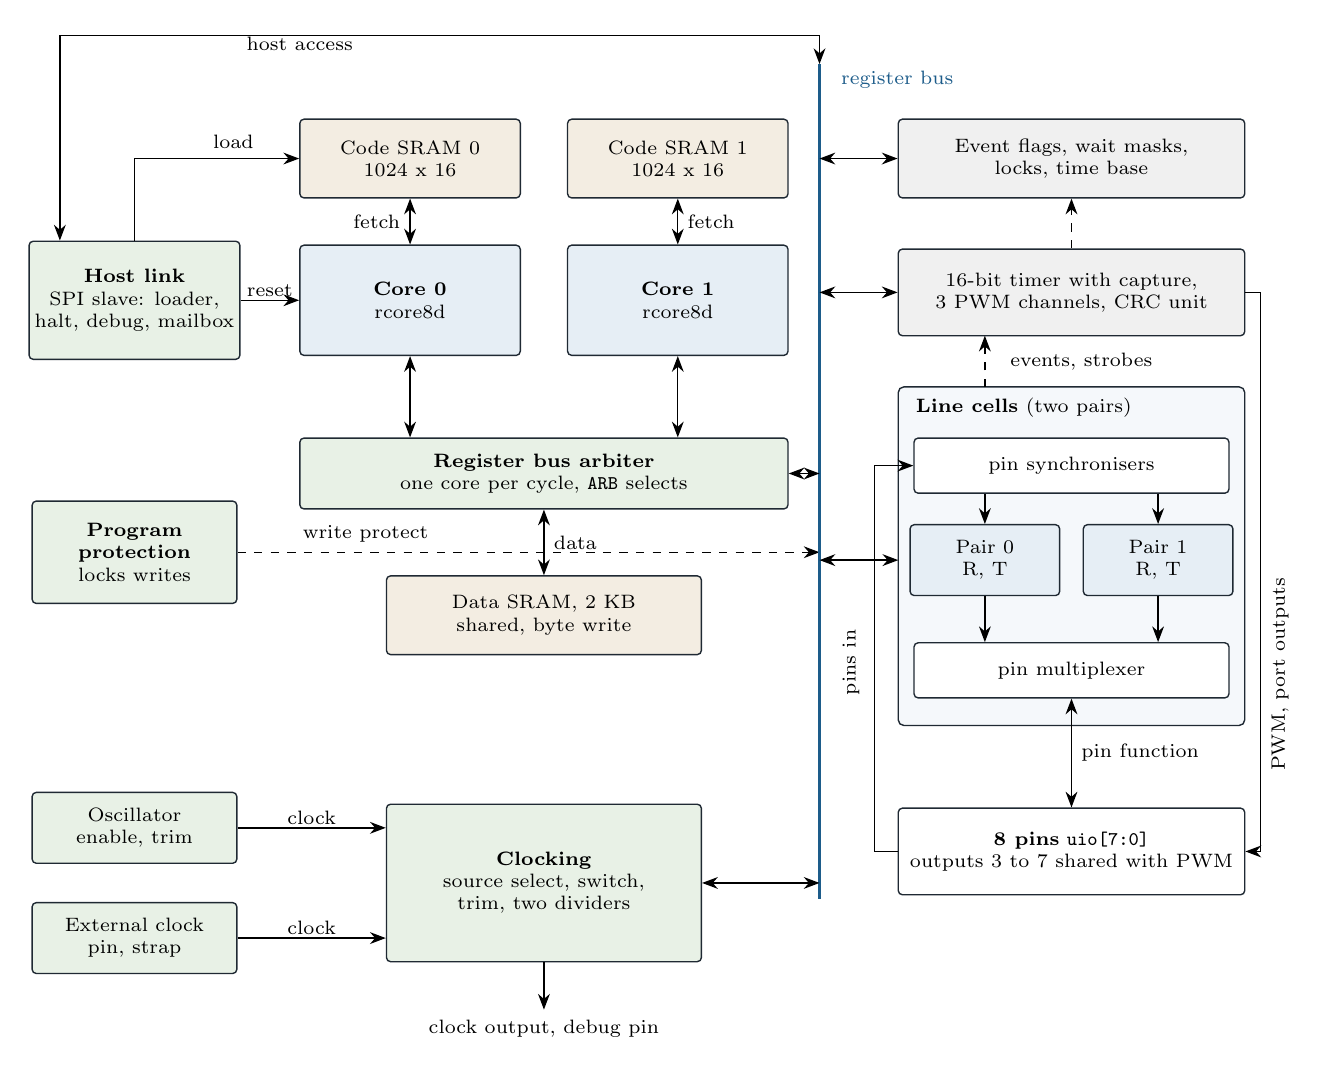
\begin{tikzpicture}[x=1mm,y=1mm,
  bk/.style={blk,font=\scriptsize,inner sep=2pt,align=center}]
  % host and protection
  \node[bk,fill=fillC,minimum width=26mm,minimum height=15mm] (host) at (17,94) {\textbf{Host link}\\ SPI slave: loader,\\ halt, debug, mailbox};
  \node[bk,fill=fillC,minimum width=26mm,minimum height=13mm] (prot) at (17,62) {\textbf{Program}\\ \textbf{protection}\\ locks writes};
  % memories and cores
  \node[bk,fill=fillB,minimum width=28mm,minimum height=10mm] (pm0) at (52,112) {Code SRAM 0\\ 1024 x 16};
  \node[bk,fill=fillB,minimum width=28mm,minimum height=10mm] (pm1) at (86,112) {Code SRAM 1\\ 1024 x 16};
  \node[bk,fill=fillA,minimum width=28mm,minimum height=14mm] (c0) at (52,94) {\textbf{Core 0}\\ rcore8d};
  \node[bk,fill=fillA,minimum width=28mm,minimum height=14mm] (c1) at (86,94) {\textbf{Core 1}\\ rcore8d};
  \node[bk,fill=fillC,minimum width=62mm,minimum height=9mm] (arb) at (69,72) {\textbf{Register bus arbiter}\\ one core per cycle, \reg{ARB} selects};
  \node[bk,fill=fillB,minimum width=40mm,minimum height=10mm] (dm) at (69,54) {Data SRAM, 2 KB\\ shared, byte write};
  \draw[dar] (pm0) -- (c0) node[midway,left,lbl]{fetch};
  \draw[dar] (pm1) -- (c1) node[midway,right,lbl]{fetch};
  \draw[dar] (c0.south) -- (c0.south |- arb.north);
  \draw[dar] (c1.south) -- (c1.south |- arb.north);
  \draw[dar] (arb) -- (dm) node[midway,right,lbl]{data};
  \draw[ar] (host.east) -- (c0.west) node[midway,above,lbl,inner sep=1pt]{reset};
  \draw[ar] (host.north) |- (pm0.west) node[pos=0.8,above,lbl]{load};
  \draw[ar,dashed] (prot.east) -- (104,62) node[pos=0.22,above,lbl]{write protect};
  % register bus
  \draw[line width=1.2pt,accent] (104,18) -- (104,124);
  \node[lbl,text=accent,anchor=west] at (105.5,122) {register bus};
  \draw[dar] (arb.east) -- (104,72);
  \draw[dar] (host.north west) ++(4,0) -- ++(0,26) -| (104,124);
  \node[lbl,anchor=south west] at (30,124.5) {host access};
  % right column
  \node[bk,fill=fillD,minimum width=44mm,minimum height=10mm] (ev) at (136,112) {Event flags, wait masks,\\ locks, time base};
  \node[bk,fill=fillD,minimum width=44mm,minimum height=11mm] (tm) at (136,95) {16-bit timer with capture,\\ 3 PWM channels, CRC unit};
  \draw[dar] (104,112) -- (ev.west);
  \draw[dar] (104,95) -- (tm.west);
  \draw[ar,dashed] (tm.north) -- (ev.south);
  % line cells
  \draw[blk,fill=fillA!40,rounded corners=2pt] (114,40) rectangle (158,83);
  \node[lbl,anchor=north west] at (115,82.8) {\textbf{Line cells} (two pairs)};
  \node[bk,fill=white,minimum width=40mm,minimum height=7mm] (sy) at (136,73) {pin synchronisers};
  \node[bk,fill=fillA,minimum width=19mm,minimum height=9mm] (p0) at (125,61) {Pair 0\\ R, T};
  \node[bk,fill=fillA,minimum width=19mm,minimum height=9mm] (p1) at (147,61) {Pair 1\\ R, T};
  \node[bk,fill=white,minimum width=40mm,minimum height=7mm] (pmx) at (136,47) {pin multiplexer};
  \draw[ar] (sy.south -| p0) -- (p0.north);
  \draw[ar] (sy.south -| p1) -- (p1.north);
  \draw[ar] (p0.south) -- (p0.south |- pmx.north);
  \draw[ar] (p1.south) -- (p1.south |- pmx.north);
  \draw[dar] (104,61) -- (114,61);
  \draw[ar,dashed] (125,83) -- (125,89.5);
  \node[lbl,anchor=west,align=left] at (127,86.2) {events, strobes};
  % pins
  \node[bk,fill=white,minimum width=44mm,minimum height=11mm] (pins) at (136,24) {\textbf{8 pins} \reg{uio[7:0]}\\ outputs 3 to 7 shared with PWM};
  \draw[dar] (pmx.south) -- (pins.north) node[midway,right,lbl]{pin function};
  \draw[ar] (pins.west) -- (111,24) -- (111,73) -- (sy.west);
  \node[lbl,anchor=south,rotate=90] at (110.3,48) {pins in};
  \draw[ar] (tm.east) -- (160,95) -- (160,24) -- (pins.east);
  \node[lbl,anchor=east,rotate=90] at (162.5,60) {PWM, port outputs};
  % clocking
  \node[bk,fill=fillC,minimum width=40mm,minimum height=20mm] (clk) at (69,20) {\textbf{Clocking}\\ source select, switch,\\ trim, two dividers};
  \node[bk,fill=fillC,minimum width=26mm,minimum height=9mm] (osc) at (17,27) {Oscillator\\ enable, trim};
  \node[bk,fill=fillC,minimum width=26mm,minimum height=9mm] (ext) at (17,13) {External clock\\ pin, strap};
  \draw[ar] (osc.east) -- (clk.west |- osc.east) node[midway,above,lbl,inner sep=1pt]{clock};
  \draw[ar] (ext.east) -- (clk.west |- ext.east) node[midway,above,lbl,inner sep=1pt]{clock};
  \draw[dar] (clk.east) -- (104,20);
  \draw[ar] (clk.south) -- ++(0,-6) node[below,lbl]{clock output, debug pin};
\end{tikzpicture}
}
\caption{Top level, as built in the RTL (module \texttt{rpe\_core}). Solid arrows are data and control paths, dashed
arrows are event and strobe paths. The core clock enable and the peripheral tick from the clocking block go to
all other blocks and are not drawn. The two cores reach the code memory of the other core only through the host
port.}
\label{fig:block}
\end{figure}

Figure~\ref{fig:block} shows the blocks. The chip has two cores. Each core fetches from a code memory of its own. The data memory and the register bus
with all peripherals are shared; an arbiter gives them to one core per cycle. The host link is fixed hardware
and works without any program. Line cells take their pins from the bidirectional port; the remaining input and
output pins are plain port bits. A build with one core and one code memory is the configuration for the
smallest product die.

\section{Choice of the CPU core}

The core was selected earlier for the small-die product and is reused here unchanged in its instruction set.
This section summarises that selection.

\subsection{Decision}

The core uses the reduced AVR instruction set (the avrtiny class of the ATtiny10, with 16 registers r16 to r31)
in a new implementation, \texttt{rcore8}. Of four candidates it produced the smallest total code size, it has a
mature C compiler, and no existing open core implements it. Binary compatibility with AVR devices is not a
requirement and is not claimed.

\subsection{Candidates}

Four instruction sets were compared. Each has a C compiler that could be used for the test.

\begin{table}[!htb]
\centering\small
\begin{tabularx}{\linewidth}{@{}l>{\raggedright\arraybackslash}p{38mm}lL@{}}
\toprule
Candidate & Type & Compiler & Assessment \\
\midrule
Padauk pdk14 & Accumulator machine, 14-bit instructions; the incumbent architecture & SDCC &
Reference point for the 2 cent market. Smallest code only on the simplest program. \\
f8 / f8l & New 8-bit architecture designed for SDCC & SDCC &
Lacks bit operations and short addressing, which small control programs use constantly. Carries instructions
with little use at this size. \\
Reduced AVR & Load-store, 16 registers, 16-bit instructions & avr-gcc &
Smallest total code. Constant tables are read directly from program memory. \\
Classic AVR & Load-store, 32 registers & avr-gcc &
Larger core. Copies constant tables to RAM at start-up, which costs code and RAM on a small die. \\
\bottomrule
\end{tabularx}
\caption{Candidate instruction sets. The PIC-like core of the Nyquest NY8A051H served as the market baseline for
die size and price and was not part of the code size comparison.}
\end{table}

\subsection{Code size comparison}

Three C programs typical for this chip class were compiled for each architecture: a candle-flicker LED, an
infrared remote transmitter and a fan controller.

\begin{table}[!htb]
\centering\small
\begin{tabular}{@{}lrrrr@{}}
\toprule
Program & pdk14 & f8 & Reduced AVR & Classic AVR \\
\midrule
candle & 187 & 193 & 196 & 206 \\
irsend & 333 & 346 & 270 & 282 \\
fanctl & 378 & 315 & 282 & 364 \\
\midrule
Total & 898 & 854 & \textbf{748} & 852 \\
Relative to reduced AVR & +20\,\% & +14\,\% & & +14\,\% \\
\bottomrule
\end{tabular}
\caption{Size of the complete program image in bytes. SDCC 4.5.2 was used for pdk14 and f8.}
\end{table}

Reduced AVR needs 12\,\% less code in total than the next candidates, and it is within 5\,\% of the best result
on the one program where it is not smallest. The comparison rests on three small programs, one compiler version
per architecture and no hand optimisation. It shows the order of the candidates, not exact ratios.

\subsection{Reasons}

\begin{itemize}
\item \textbf{Code size.} The smallest total code means the least program memory for a given function, and
memory is the largest block on the small die. In this design each code macro takes about 2.9 tiles.
\item \textbf{Compiler.} avr-gcc supports the instruction set today, so no compiler work is needed.
\item \textbf{Register file.} Sixteen registers halve the register file compared with classic AVR. With two cores this saving applies twice.
\item \textbf{Constants stay in program memory.} Classic AVR copies them to RAM at start-up.
\item \textbf{Bit operations.} Bit set, bit clear and bit test on I/O registers are single instructions, which
f8 lacks. Protocol code uses them constantly.
\item \textbf{pdk14} is best only on the smallest program, and using the incumbent's instruction set offers no
technical advantage over the incumbent.
\item \textbf{Classic AVR} remains the candidate for a later, larger die.
\end{itemize}

\subsection{New implementation}

\begin{itemize}
\item A search for open cores found no implementation of the reduced 16-register set. Navr\'e implements
classic AVR and was synthesised against the GF180MCU library as a size reference.
\item A new core could be built for the purpose: two-stage fetch and execute with a synchronous program memory,
masked single-bit I/O writes, and an interface that fits the peripheral block.
\item \textbf{Status.} \texttt{rcore8} exists as Verilog and passes its tests in simulation: 1.76 million random
instructions in lockstep with a Python reference model, C test programs and gate-level simulation. It occupies
0.0436\,mm$^2$ after synthesis for GF180MCU. No timing analysis has been done.
\item \textbf{Options} of the core are the program counter width, RAM size, number of interrupts and the
half-carry flag.
\end{itemize}

The selection covers the small die. It should be repeated with the firmware of the lead application once that
is chosen, and a legal check of the instruction set and of any use of the AVR name is needed before a product
is sold.

\section{Cores}\label{sec:cores}

\subsection{Basis}

Each core is \texttt{rcore8}: the 16-register reduced AVR instruction set (ATtiny4/5/9/10/20/40 class), usable
with \texttt{avr-gcc -mmcu=attiny40}. All instructions are one word. The instruction semantics are not changed,
so the existing Python model and the lockstep tests continue to apply to each core.

The core keeps its pipeline: the next sequential instruction is fetched while the current one executes, most
instructions take one cycle, and a taken branch costs one more. Three things are added: a clock enable, a
synchronous read of the data memory, and the ninth address bit of the register bus.

A generic synthesis of the present core gives 3\,860 two-input gates including 180 flip-flops
(\texttt{PC\_W}=10, \texttt{RAM\_AW}=9). Of these, 1\,900 are the register file. The core as used here, with an 11-bit program counter, maps to 2\,280 cells of the IHP library with a cell area of 30\,100\,$\mu$m$^2$. Both cores with the arbiter and the core control registers map to 4\,985 cells and 69\,000\,$\mu$m$^2$ (yosys, slow corner library, no timing-driven sizing); with the host port and the injection sequencer added later the block is 5\,721 cells and 77\,400\,$\mu$m$^2$ (section~\ref{sec:hostver}).

\subsection{Two cores, private code, shared data}

\begin{itemize}
\item \textbf{Code memory.} Each core has its own 1024-word macro. Both cores therefore fetch in every cycle and
run at the full clock rate at the same time.
\item \textbf{Shared bus.} The data memory and the register bus form one resource. A core requests it only in
cycles in which its instruction accesses data or a register.
\item \textbf{Arbitration.} If both cores request the shared bus in the same cycle, one gets it and the other is
held for that cycle through its clock enable. Because its code memory is private, a held core loses nothing but
the cycle.
\item \textbf{Modes.} A register selects who wins a collision: always core 0, always core 1, or alternating.
\item \textbf{Exact timing.} The core that always wins is never held. The number of clock cycles its program
takes depends only on the program. This is the mode for protocol timing in firmware.
\item \textbf{Start.} After reset only core 0 runs. Core 0 or the host starts core 1.
\item \textbf{Bypass.} Each core can read and write the other core's code memory through the data address
space. This path is slow, because it takes the other core's fetch port for a cycle.
\item \textbf{One core alone.} While core 1 is stopped, core 0 can execute from both code memories as one
program space of 2K words.
\end{itemize}

\begin{figure}[!htb]
\centering
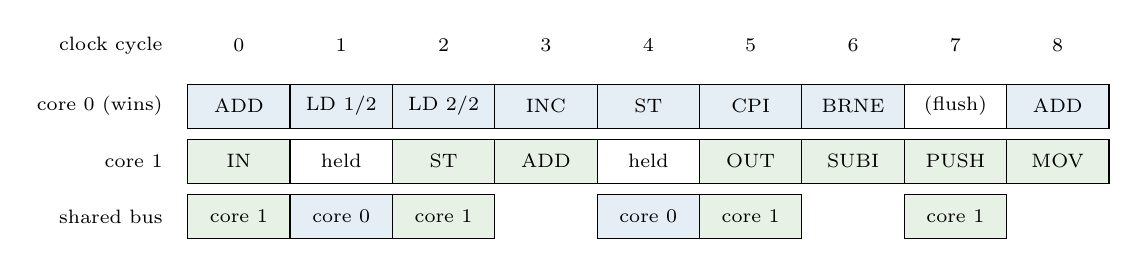
\begin{tikzpicture}[x=13mm,y=7mm]
  \foreach \c in {0,...,8} { \node[lbl] at (\c+0.5,3.6) {\c}; }
  \node[lbl,anchor=east] at (-0.15,3.6) {clock cycle};
  \foreach \r/\name in {2/{core 0 (wins)},1/{core 1},0/{shared bus}} {
    \node[lbl,anchor=east] at (-0.15,\r+0.5) {\name};
  }
  % core 0
  \foreach \c/\t/\f in {0/ADD/fillA,1/{LD 1/2}/fillA,2/{LD 2/2}/fillA,3/INC/fillA,4/{ST}/fillA,5/CPI/fillA,6/{BRNE}/fillA,7/{(flush)}/white,8/ADD/fillA} {
    \draw[fill=\f] (\c,2.1) rectangle ++(1,0.8) node[midway,lbl]{\t};
  }
  % core 1
  \foreach \c/\t/\f in {0/{IN}/fillC,1/{held}/white,2/{ST}/fillC,3/ADD/fillC,4/{held}/white,5/{OUT}/fillC,6/SUBI/fillC,7/{PUSH}/fillC,8/MOV/fillC} {
    \draw[fill=\f] (\c,1.1) rectangle ++(1,0.8) node[midway,lbl]{\t};
  }
  % bus
  \foreach \c/\t/\f in {0/{core 1}/fillC,1/{core 0}/fillA,2/{core 1}/fillC,4/{core 0}/fillA,5/{core 1}/fillC,7/{core 1}/fillC} {
    \draw[fill=\f] (\c,0.1) rectangle ++(1,0.8) node[midway,lbl]{\t};
  }
\end{tikzpicture}
\caption{Example with priority for core 0. In cycles 1 and 4 both cores request the shared bus; core 1 is held
and repeats its request in the next cycle. Core 0 runs as if it were alone. LD takes two cycles and uses the bus in the first.}
\label{fig:sched}
\end{figure}

\begin{table}[!htb]
\centering\small
\begin{tabularx}{\linewidth}{@{}Lc@{}}
\toprule
Instruction & Cycles \\
\midrule
ALU, MOV, LDI, IN, OUT, SBI, CBI, bit operations; ST, STS, PUSH; LD from a register; branch not taken; skip that does not skip & 1 \\
Taken branch, RJMP, IJMP, skip that skips; RCALL, ICALL; interrupt entry & 2 \\
LD, LDS, POP from the data memory & 2 \\
RET, RETI & 3 \\
LD from the core's own code memory; ST to it, enabled or not & 3 \\
\bottomrule
\end{tabularx}
\caption{Instruction durations in cycles in which the core is enabled. Cycles in which the core is held by the
arbiter are added. At 60\,MHz a core executes up to 60 million one-cycle instructions per second.}
\label{tab:dur}
\end{table}

\subsection{Interrupts and waiting}

\begin{itemize}
\item \textbf{Interrupts} exist on both cores. Each core has its own I flag and its own enable mask over the
shared event flags. While a core has interrupts enabled, its timing is not exact.
\item \textbf{Waiting.} Each core has a wait mask register. Writing a mask stops the core until one of the
selected event flags is set (section~\ref{sec:events}). The core continues in the cycle after that.
\item An enabled interrupt that is pending ends a wait, as it ends SLEEP in the present core.
\item A waiting core does not request the shared bus. When both cores wait, the core clock can stop. This is the
sleep mode of the product.
\end{itemize}

\subsection{Why not thread contexts on one core}

Earlier drafts shared one decoder and ALU between up to four thread contexts, selected by a slot table. That
design was built and tested (\texttt{rcore8t}) and then dropped, for these measured reasons:

\begin{itemize}
\item Half of the core is its register file, which every context needs for itself. A context cost about 3\,400
two-input gates including 215 flip-flops, against 3\,860 for a complete core. Two contexts (9\,463 gates) were
larger than two cores.
\item One code memory delivers one word per cycle. Two threads got 30\,MIPS each at 60\,MHz, four got 15.
\item What the contexts saved was the second code memory, about 2.9 tiles.
\end{itemize}

With separate code memories both cores run at the full clock rate, the core that wins collisions has exact
timing at that rate, and the core RTL stays close to the verified \texttt{rcore8}.

\section{Core behaviour}\label{sec:corebeh}

This section defines the sequencing of the two cores as numbered rules. The instruction semantics, including
the flags, are those of the existing \texttt{rcore8} and its Python model and are not repeated.

All cycles in this section are cycles in which the core clock is enabled by the core divider.

\subsection{Pipeline}

\begin{enumerate}[label=\textbf{P\arabic*},leftmargin=2.6em]
\item \textbf{Fetch and execute.} While an instruction executes, the core presents the next sequential address to
its code memory. The word is on the memory output in the following cycle.
\item \textbf{Enable.} A core advances in a cycle only if it is enabled. It is not enabled while it is stopped,
waiting or halted, and in a cycle in which it is held (rules U3 and U7). In such a cycle its state does not
change and its code memory is not read, so the memory output keeps the fetched word.
\item \textbf{Durations} in enabled cycles are those of table~\ref{tab:dur}. After a taken branch, a jump, a call
or a skip that skips, the word already fetched is discarded and one cycle is lost.
\item \textbf{Data memory read.} The address is presented in the first cycle. The byte is on the data memory
output in the second cycle and is written to the destination register at the end of it. The next instruction
executes in the third cycle.
\item \textbf{Calls.} RCALL, ICALL and the interrupt entry push the low byte of the return address in the first
cycle and the high byte in the second.
\item \textbf{Returns.} RET and RETI read the high byte in the first cycle and the low byte in the second. In the
third cycle the low byte is on the data memory output; it is passed directly to the code memory address and
written to the program counter.
\item \textbf{Own code memory as data.} A load reads the word in the second cycle in place of a fetch, writes the
selected byte to the register and fetches the next instruction again in the third. A store writes in the second cycle in place of a fetch and fetches the next instruction again in the third.
\end{enumerate}

\subsection{Shared bus}

\begin{enumerate}[label=\textbf{U\arabic*},leftmargin=2.6em]
\item \textbf{Request.} A core requests the shared bus in every cycle in which it presents an address to the data
memory or accesses a register: the first cycle of LD, LDS and POP; ST, STS and PUSH; both cycles of a call or
an interrupt entry; the first two cycles of a return; IN and OUT except to \reg{SREG}, \reg{SPL}, \reg{SPH}
and \reg{CCP}; SBI, CBI, SBIC and SBIS. The request depends only on the instruction and its cycle; a load or store through a pointer requests the bus in its first cycle also when the address turns out to be in a code memory.
\item \textbf{Grant.} If one core requests, it is granted. If both request, \reg{ARB.MODE} decides: 1 grants to
core 0, 2 to core 1, and 0 to the core that was not granted in the previous collision.
\item \textbf{Hold.} A core that requests and is not granted is held for the cycle (rule P2). It requests again
in the next cycle.
\item \textbf{Read data.} The byte of a data memory read is taken by the reading core in the cycle after the
grant. The core does not need the bus in that cycle, and the other core may use it. The byte is taken even if
the reading core is held in that cycle for another reason.
\item \textbf{Exact timing.} With \reg{MODE} 1 or 2 the named core is never held by rule U3. Its duration in
clock cycles depends only on its program and on its own interrupts.
\item \textbf{Bound.} With \reg{MODE} 0 a core is held for at most one cycle per requesting cycle.
\item \textbf{Other core's code memory.} A load or store whose address lies in the other core's code memory uses
that memory's port for one cycle. If the owner is running, it is held in that cycle and in the next one, in
which its code memory reads again the word that the owner had fetched last. If the owner is stopped, waiting
or halted, it is not affected at the time; when it continues, its first cycle is used for the same re-read. If
the owner is the core named by \reg{MODE} 1 or 2 and is running, the accessing core is held until the owner is
stopped, waiting or halted. If both cores start such an access in the same cycle, core 0 goes first.
\item \textbf{One access per cycle.} At most one core uses the data memory port and the register bus in a cycle.
Its number is the core number on the bus. Every instruction that accesses a register or a byte of memory is
therefore atomic with respect to the other core.
\end{enumerate}

\subsection{Address decoding}

\begin{table}[H]
\centering\small
\begin{tabularx}{\linewidth}{@{}llL@{}}
\toprule
Data address & Target & Rule \\
\midrule
bit 14 set & Code memory & Bit 11 selects the memory of core 0 or core 1, bits 10 to 1 the word, bit 0 the byte. The addresses are the same for both cores. Read always; write only by the protection rules \\
\texttt{0x3F00} to \texttt{0x3FFF} & Configuration page & Bits 13 to 8 all ones. Register bus with bit 8 of its address set \\
\texttt{0x0000} to \texttt{0x003F} & Fast I/O & Bits 13 to 6 all zero. Register bus \\
all other & Data memory & Byte address = bits 10 to 0 \\
\bottomrule
\end{tabularx}
\caption{Decoding of a data address, checked in this order.}
\end{table}

\begin{enumerate}[label=\textbf{M\arabic*},leftmargin=2.6em]
\item The data memory is not offset. Data addresses \texttt{0x0040} to \texttt{0x07FF} select the bytes with the
same number, and \texttt{0x0800} to \texttt{0x083F} select bytes 0 to 63. The range \texttt{0x0040} to
\texttt{0x083F} is therefore contiguous. Other addresses that fall on the data memory must not be used.
\item \reg{SREG}, \reg{SPL}, \reg{SPH} and \reg{CCP} are reached with IN and OUT only, as in the existing core. A
load or store to their data addresses goes to the register bus and finds no register.
\item The stack pointer has 12 bits. PUSH writes at the stack pointer and then decrements it; POP increments it and
then reads. Stack accesses always go to the data memory, at the low 11 bits of the stack pointer.
\item A store to a code memory is carried out if \reg{PMCR.LOCK} is clear, the word address is not below four
times \reg{PMLIM}, and \reg{PMCR.PWE} is set for the core's own memory or \reg{PMCR.XWE} for the other core's.
Otherwise it is ignored; it takes the same number of cycles.
\item \textbf{Program counter.} Core 1 has 10 bits and executes from its own code memory only. Core 0 has 11 bits;
bit 10 selects the code memory of core 1. Core 0 fetches from that memory only while core 1 is stopped; otherwise it is held until core 1 is stopped. Core 0 must not be executing there when core 1 is started.
\end{enumerate}

\subsection{Core control}

\begin{enumerate}[label=\textbf{H\arabic*},leftmargin=2.6em]
\item \textbf{Reset.} Core 0 is enabled with its program counter at 0. Core 1 is stopped. The flags are cleared.
The stack pointer is \texttt{0x083F} in core 0 and \texttt{0x043F} in core 1. The registers r16 to r31 are not
reset.
\item \textbf{Start.} When an enable bit in \reg{CORECTL} changes from 0 to 1, the core's program counter is set
to 0, and its wait state and unlock window are cleared. Registers, flags and stack pointer keep their values.
\item \textbf{Stop.} When the bit changes from 1 to 0, the core does not advance any more, also in the middle of an instruction. It can only be started again from address 0. A core can stop itself and the other core.
\item \textbf{Wait.} An OUT to \reg{WAITL} stores the mask and puts the core into the wait state at the end of the
cycle. In every cycle the 16-bit mask is compared with the event flags as the core sees them. The core is
enabled again in the cycle after one in which a selected flag was set. If a selected flag is already set when
the mask is written, the core does not wait.
\item \reg{WAITL} and \reg{WAITH} read back the mask. The core finds the reason for the end of a wait in
\reg{IFR}.
\item \textbf{SLEEP} puts the core into the wait state with the mask it wrote last. The wait also ends when an
enabled interrupt of the core is pending.
\item \textbf{BREAK} halts the core and sets its break flag for the host link. WDR is executed as NOP.
\item \textbf{Halt.} The host link halts and releases the cores individually. A halted core does not advance; it continues from the same cycle when it is released. The host can have a halted core execute one instruction that it supplies; the program counter is not incremented for it (rules L8 to L10, implemented in \texttt{rdual.v}).
\item \textbf{Core clock.} If no core is enabled because both are stopped, waiting or halted, the core clock can
be gated until a wait ends, an interrupt is pending or the host link acts. \texttt{rdual} provides the signal \texttt{idle} for this; it is not connected to a clock gate in this draft, so the core clock is not gated.
\item \textbf{Core number.} \reg{CORECTL.ID} reads as the number of the reading core. A program that is loaded into
both code memories uses it to branch.
\end{enumerate}

\subsection{Interrupts and protected writes}

\begin{enumerate}[label=\textbf{Q\arabic*},leftmargin=2.6em]
\item Each core has an I flag and an enable mask \reg{IER}. The request for vector $n+1$ is flag $n$ of
\reg{IFR}, as the core sees it, and bit $n$ of the core's \reg{IER}. The lowest pending vector is taken. The
vector is word address $n+1$ of the core's code memory.
\item An interrupt is taken in a cycle that would start a new instruction, if I is set. The instruction is
discarded and its address is the return address. I is cleared. Entry takes two cycles.
\item After an instruction that sets I, one more instruction executes before an interrupt is taken, as in the
existing core.
\item A flag that is cleared by writing a one is not cleared by taking its interrupt, except the five timer and
pin-change flags \reg{PC}, \reg{CAPT}, \reg{OCA}, \reg{OCB} and \reg{OVF}, which are cleared on entry as in
\texttt{rperiph}. If both cores enable the same flag, both take the interrupt only if the second sees the flag
before the entry of the first clears it; one flag should be enabled on one core.
\item \textbf{Unlock window.} Each core has a counter. An OUT of \texttt{0xD8} to \reg{CCP} sets it to 4. It is
decremented when the core completes an instruction. A write to a protected register is carried out only if
the writing core's counter is not zero, and it clears the counter.
\end{enumerate}

\subsection{Deviations kept from the existing core}

\begin{itemize}
\item The S flag is not stored. It reads as N exclusive-or V.
\item The H flag exists only if the build option is set.
\item Undefined opcodes execute as NOP. All instructions are one word.
\item SBI and CBI write a single bit without reading the register.
\item Timing differs from the Microchip parts.
\end{itemize}

\subsection{Paths that set the clock frequency}

\begin{itemize}
\item Code memory output, decode, register file, pointer adder, arbiter multiplexer, data memory address.
\item Code memory output, decode, register bus address, arbiter multiplexer, read multiplexer, ALU, register
file.
\item Code memory output of both cores, decode of the bus request, arbiter, clock enable of all core
flip-flops.
\item Data memory output to code memory address, for the return address (rule P6).
\end{itemize}

If these paths do not meet 60\,MHz, the core divider is set to 2 as a build option. The cores then run at
30\,MHz, their paths are two-cycle paths, and the line cells and timers stay at 60\,MHz
(section~\ref{sec:clock}).

\subsection{Implementation and verification}\label{sec:corever}

The rules of this section are implemented in \texttt{rcore8d.v} (one core) and \texttt{rdual.v} (two cores,
arbiter, code memory routing, \reg{CORECTL}, \reg{LOCK}, \reg{WAIT}, \reg{ARB}). A cycle model in Python,
built on the instruction model of \texttt{rcore8}, was written from the same rules.

\begin{table}[H]
\centering\small
\begin{tabularx}{\linewidth}{@{}LL@{}}
\toprule
Test & Result \\
\midrule
Random programs on both cores, 360 seeds of 4\,000 cycles; every instruction start and the final content of all memories compared with the model & no difference in 1.16 million instruction starts; 62\,700 collisions, 12\,200 accesses to the other core's code memory, 369 interrupt entries \\
Directed: locks, software flags, waits and wake-up, SLEEP ended by an interrupt from the other core, load and store in both code memories & RTL equals model; expected values in memory \\
Exact timing: core 1 with priority, core 0 either using the bus continuously or waiting & the 604 instruction starts of core 1 fall on the same cycles in both runs \\
Stress loop of calls, returns, loads and pops on both cores, in the three arbitration modes & RTL equals model \\
Compiled C tests of \texttt{rcore8} (four parts) on core 0; part 1 is 2\,844 bytes and runs across both code memories & all pass \\
Eight faults inserted into the RTL & six detected; the other two change behaviour only when the host halts a core \\
Core clock enable in every second or third cycle (core divider): random, directed, exact-timing and stress tests repeated & no difference (section~\ref{sec:clk30}) \\
\bottomrule
\end{tabularx}
\caption{Verification of the two-core RTL.}
\end{table}

\begin{table}[H]
\centering\small
\begin{tabular}{@{}lrr@{}}
\toprule
Arbitration mode & Core 0 & Core 1 \\
\midrule
Core 1 alone (core 0 waiting) & -- & 6\,757 \\
Core 0 always wins & 6\,755 & 10\,130 \\
Core 1 always wins & 10\,127 & 6\,757 \\
Alternating & 8\,554 & 8\,557 \\
\bottomrule
\end{tabular}
\caption{Clock cycles from the start of core 1 until each core has finished the stress loop, from the cycle
model. The loop uses the shared bus in about half of its cycles. Code that uses the bus less is slowed down
less.}
\end{table}

Not covered here: the protected-register input, 16 interrupt lines (this testbench uses 4), and a build with one core. Halting by the host and instruction injection are covered in section~\ref{sec:hostver}. The model and the RTL were written by the same author from the
same rules, so a misreading of a rule would be in both.

\section{Memory}

\begin{figure}[!htb]
\centering
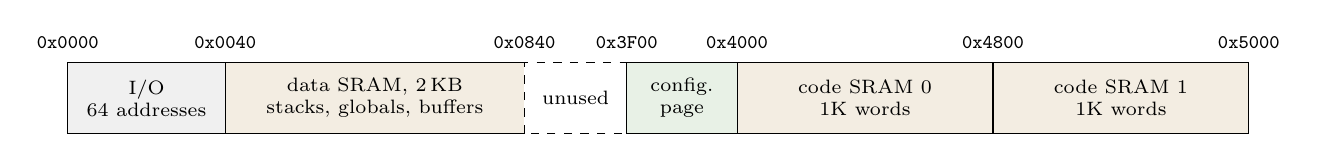
\begin{tikzpicture}[x=1mm,y=1mm]
  \draw[fill=fillD] (0,0) rectangle (20,9) node[midway,lbl]{I/O\\ 64 addresses};
  \draw[fill=fillB] (20,0) rectangle (58,9) node[midway,lbl]{data SRAM, 2\,KB\\ stacks, globals, buffers};
  \draw[fill=white,dashed] (58,0) rectangle (71,9) node[midway,lbl]{unused};
  \draw[fill=fillC] (71,0) rectangle (85,9) node[midway,lbl]{config.\\ page};
  \draw[fill=fillB] (85,0) rectangle (117.5,9) node[midway,lbl]{code SRAM 0\\ 1K words};
  \draw[fill=fillB] (117.5,0) rectangle (150,9) node[midway,lbl]{code SRAM 1\\ 1K words};
  \node[lbl,anchor=south] at (0,9.5) {\texttt{0x0000}};
  \node[lbl,anchor=south] at (20,9.5) {\texttt{0x0040}};
  \node[lbl,anchor=south] at (58,9.5) {\texttt{0x0840}};
  \node[lbl,anchor=south] at (71,9.5) {\texttt{0x3F00}};
  \node[lbl,anchor=south] at (85,9.5) {\texttt{0x4000}};
  \node[lbl,anchor=south] at (117.5,9.5) {\texttt{0x4800}};
  \node[lbl,anchor=south] at (150,9.5) {\texttt{0x5000}};
\end{tikzpicture}
\caption{Data address space, the same for both cores (not to scale). It follows the layout avr-gcc expects for
the reduced core, so the stock linker script for the ATtiny40 class applies, with the RAM size and the stack
top set by linker symbols.}
\end{figure}

\begin{table}[!htb]
\centering\small
\begin{tabular}{@{}lllrr@{}}
\toprule
Role & Macro & Capacity & Footprint ($\mu$m) & Tiles (with keep-out\est) \\
\midrule
Code, core 0 & \texttt{RM\_IHPSG13\_1P\_1024x16\_c2\_bm\_bist} & 1K words & $236.8 \times 336.5$ & 2.5 (2.9) \\
Code, core 1 & \texttt{RM\_IHPSG13\_1P\_1024x16\_c2\_bm\_bist} & 1K words & $236.8 \times 336.5$ & 2.5 (2.9) \\
Data, shared & \texttt{RM\_IHPSG13\_1P\_1024x16\_c2\_bm\_bist} & 2\,KB & $236.8 \times 336.5$ & 2.5 (2.9) \\
\bottomrule
\end{tabular}
\caption{SRAM macros. Footprints are from the LEF files of the IHP Open PDK. The keep-out figure assumes
$10\,\mu$m on each side.}
\label{tab:macros}
\end{table}

\begin{itemize}
\item The IHP macros are permitted by the competition and pass the Tiny Tapeout CMOS5L precheck (reported for the
1024x8 macro; another public entry hardened three 512x16 macros with a clean precheck).
\item The data macro is 16 bits wide and is used byte-wise through its bit mask.
\item All three memories use the same macro, so there is one macro type to place and to connect to the power
grid.
\item 2\,KB of data memory holds a full-size Ethernet frame of 1518 bytes and leaves about 500 bytes for stacks
and variables. Both cores have their stacks in it.
\item \textbf{Program images.} Each core runs the image in its own code memory. A routine used by both cores exists
in both images. Variables used by both cores are placed at addresses that both links agree on. Loading the
same image into both memories gives one program for both cores; it reads its core number from
\reg{CORECTL.ID}.
\item \textbf{One core.} With core 1 stopped, core 0 has both code memories as one space of 2K words
(rule M5).
\end{itemize}

\subsection{Code memory protection}

Normally only the host link writes the code memories, while the cores are in reset or halted. Firmware can
write them through the following mechanism, which follows the configuration change protection of the reduced
AVR core.

\begin{itemize}
\item \textbf{Direct store.} A store to \texttt{0x4000} and above writes one byte of a code word, selected by the
macro's bit mask.
\item \textbf{Enable bits.} Stores are ignored unless the write-enable bit is set: one bit for a core's own
memory, one for the other core's.
\item \textbf{Unlock.} The control register can only be changed if the same core wrote the signature to
\reg{CCP} (\texttt{0x3C}) within the preceding four instructions.
\item \textbf{Limit register.} Stores below a set word address are always ignored. This protects resident code.
\item \textbf{Sticky lock.} A bit that disables code writes until reset.
\end{itemize}

A core that fetches a word after the other core has written it gets the new word. The mechanism
takes 95 cells and 1\,300\,$\mu$m$^2$ in the synthesis (module \texttt{rprot}, section~\ref{sec:hostver}).

\section{Communication between the cores}\label{sec:comm}

The cores exchange data and synchronise through shared resources. No instruction is added for this: every
mechanism is a register or a memory address, so that avr-gcc and its assembler stay unchanged.

\begin{table}[H]
\centering\small
\begin{tabularx}{\linewidth}{@{}>{\raggedright\arraybackslash}p{33mm}>{\raggedright\arraybackslash}p{38mm}L@{}}
\toprule
Mechanism & Where & Use \\
\midrule
Shared data memory & \texttt{0x0040} to \texttt{0x083F} & Buffers and variables. The fastest path: no copy between the cores \\
Software event flags & \reg{SW0} to \reg{SW3} in \reg{IFR} & One core signals the other. The receiver waits on the flag or takes it as an interrupt \\
Wait mask & \reg{WAIT} & A core stops until a flag is set, without using cycles or the shared bus \\
Locks & \reg{LOCK}, four bits & Mutual exclusion for data that needs more than one access \\
Core control & \reg{CORECTL} & Start and stop the other core; read the own core number \\
Line cell owner & \reg{LCOWN} & Hand a pair of line cells with its pins from one core to the other \\
Time base & read of \reg{DLY} & A common clock for both cores; time stamps and deadlines agree \\
Other core's code memory & \texttt{0x4000}, \texttt{0x4800} & Read tables or load code for the other core. Slow \\
CRC unit owner & \reg{CRCCTL.OWNER} & One core at a time uses the unit \\
\bottomrule
\end{tabularx}
\caption{Mechanisms for communication between the cores. The host mailbox is a channel to the host and is not
listed.}
\end{table}

\subsection{What is atomic}

\begin{enumerate}[label=\textbf{C\arabic*},leftmargin=2.6em]
\item One access to a byte of data memory or to a register is atomic (rule U8). This includes SBI and CBI, which
write one bit without reading the register.
\item A sequence of instructions is not atomic: read, modify and write of a byte in memory, or any access to a
16-bit variable. The other core can access the same location between two instructions.
\item The high-byte latch of the 16-bit registers exists once per core. A 16-bit register access by one core is
not disturbed by the other.
\item An event flag that is set before a core writes its wait mask is not lost: the core then does not wait
(rule H4).
\end{enumerate}

\subsection{Software event flags}

\begin{itemize}
\item \textbf{Set and clear.} A core sets a flag with SBI and clears it with CBI on \reg{IFRH}. Both cores see
the same four flags.
\item \textbf{Wake-up.} The receiving core includes the flag in its wait mask. It is enabled again in the cycle
after the flag is set.
\item \textbf{Interrupt.} A core that sets the flag's bit in its \reg{IER} takes the flag as an interrupt. This
is a software interrupt from one core to the other.
\item \textbf{Convention.} With four flags, two per direction are available. A flag carries no data; the data is
in the shared memory.
\end{itemize}

\subsection{Locks}

\begin{enumerate}[label=\textbf{C\arabic*},leftmargin=2.6em,start=5]
\item \reg{LOCK} holds four locks. Each lock is free or held by one core.
\item A core takes lock $n$ by writing a one to bit $n$. The write has an effect only if the lock is free. The
core then reads the bit: it is one only if the reading core holds the lock.
\item A core releases a lock by writing a zero to its bit. The write has an effect only if the writing core holds
the lock.
\item Two cores cannot write in the same cycle (rule U8), so no further arbitration is needed.
\item Bits 4 to 7 read as one if the other core holds the lock.
\item A core that is stopped or started keeps its locks. Reset frees all locks.
\end{enumerate}

\begin{verbatim}
take:  sbi  LOCK, 0          ; request lock 0
       sbis LOCK, 0          ; held by this core?
       rjmp take             ; no: the other core has it
       ...                   ; access the shared data
       cbi  LOCK, 0          ; release
\end{verbatim}

A lock is not needed for a ring buffer with one writing and one reading core, if each index is one byte and is
written by one core only.

\subsection{Shared data and a frame hand-over}

A typical use: core 1 receives a frame into the shared memory with exact timing, core 0 processes it.

\begin{verbatim}
; core 1: receiver
rx:    ...                   ; receive into buf
       sts  len, r24
       sbi  IFRH, 4          ; set SW0: frame ready
       ldi  r20, 0x20        ; mask: SW1
       out  WAITH, r20
       out  WAITL, r17       ; wait (r17 = 0)
       cbi  IFRH, 5          ; clear SW1
       rjmp rx

; core 0: processing
main:  ldi  r20, 0x10        ; mask: SW0
       out  WAITH, r20
       out  WAITL, r17       ; wait
       cbi  IFRH, 4          ; clear SW0
       ...                   ; process buf, len
       sbi  IFRH, 5          ; set SW1: buffer free
       rjmp main
\end{verbatim}

\subsection{Line cells, time base and code memory}

\begin{itemize}
\item \textbf{Line cell hand-over.} The owning core disables the cells of a pair; either core rewrites \reg{LCOWN} with the unlock sequence. The other core then has access to the pair, with its configuration and pins unchanged.
\item \textbf{Time base.} Both cores read the same 16-bit counter. A time stamp taken by one core can be used
as a wake-up time by the other.
\item \textbf{Code memory.} A core reads constant tables from either code memory. With \reg{PMCR.XWE} set, core 0
can load a program for core 1 and then start it. Each access holds the other core for two cycles if it is running (rule U7).
\end{itemize}

\subsection{Not included}

\begin{itemize}
\item \textbf{Special instructions.} None. The instruction set stays that of the reduced AVR core.
\item \textbf{Hardware FIFO or message register between the cores.} The shared memory with a software flag does
the same without a copy.
\item \textbf{A way to hold the other core for several instructions.} It would remove the exact timing of the
core that wins collisions. The locks cover mutual exclusion.
\item \textbf{An event flag for a released lock.} A core that finds a lock taken repeats the request or waits on
a software flag by convention with the other core.
\end{itemize}

\section{Line cells}

There are two receive cells and two transmit cells. One receive cell and one transmit cell form a pair, and a
pair serves one protocol port. A cell has no program and no sequencer beyond two control states: waiting, or
timing.

A first version combined receiver and transmitter in one cell, four times. It was built and measured at
24\,700\,$\mu$m$^2$ per cell. Most protocols use the two halves in different cells, because each needs the
timer, so half of each cell was idle. The split cells keep every function and take 55\,\% of the area. Figure~\ref{fig:pair} shows a pair with its
inputs, outputs and links.

\begin{figure}[!htb]
\centering
\resizebox{\textwidth}{!}{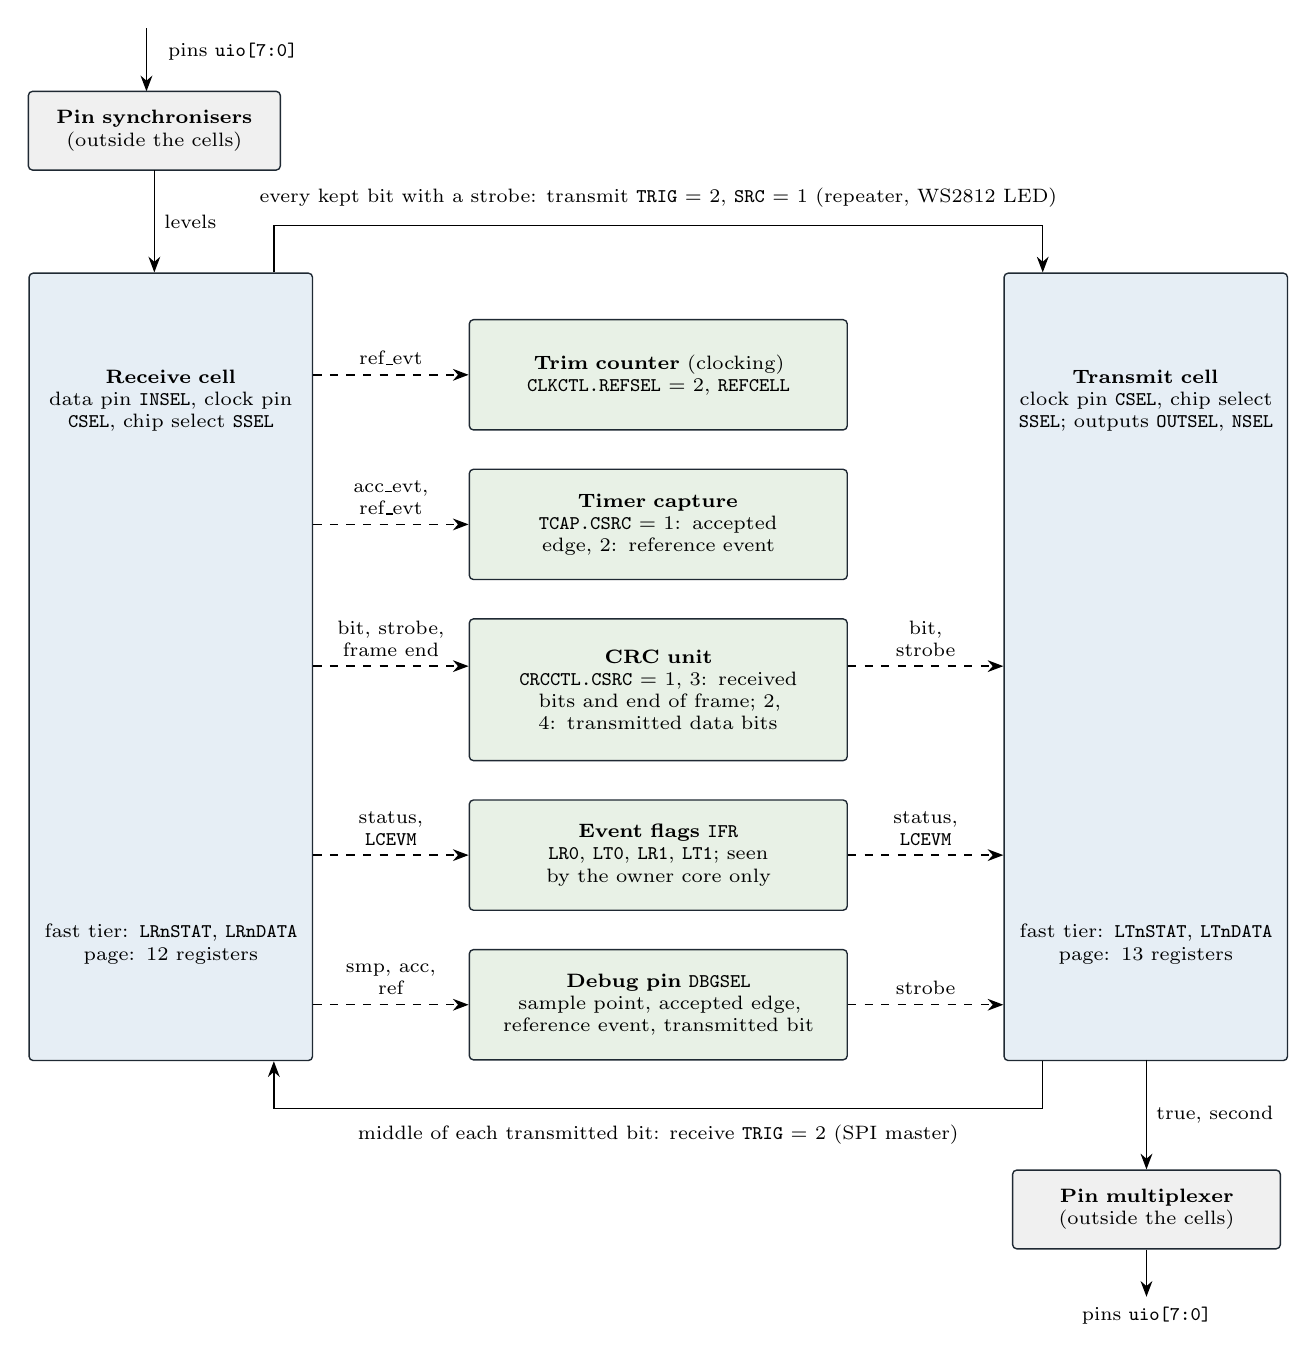
\begin{tikzpicture}[x=1mm,y=1mm,
  b/.style={blk,font=\scriptsize,inner sep=2pt,minimum height=14mm,minimum width=48mm,text width=45mm},
  ev/.style={ar,dashed}]
  % pins and synchronisers
  \draw[ar] (15,144) -- (15,136) ;
  \node[lbl,anchor=west] at (16.5,141) {pins \texttt{uio[7:0]}};
  \node[blk,fill=fillD,font=\scriptsize,inner sep=2pt,minimum width=32mm,text width=30mm,minimum height=10mm] (sy) at (16,131) {\textbf{Pin synchronisers}\\ (outside the cells)};
  \draw[ar] (16,126) -- (16,113) node[pos=0.5,right,lbl]{levels};
  % cells
  \node[blk,fill=fillA,anchor=north west,minimum width=36mm,minimum height=100mm,align=center,font=\scriptsize,text width=33mm,inner sep=2pt] (R) at (0,113) {\textbf{Receive cell}\\ data pin \reg{INSEL}, clock pin \reg{CSEL}, chip select \reg{SSEL}\\[62mm] fast tier: \reg{LRnSTAT}, \reg{LRnDATA}\\ page: 12 registers};
  \node[blk,fill=fillA,anchor=north east,minimum width=36mm,minimum height=100mm,align=center,font=\scriptsize,text width=33mm,inner sep=2pt] (T) at (160,113) {\textbf{Transmit cell}\\ clock pin \reg{CSEL}, chip select \reg{SSEL}; outputs \reg{OUTSEL}, \reg{NSEL}\\[62mm] fast tier: \reg{LTnSTAT}, \reg{LTnDATA}\\ page: 13 registers};
  % consumers
  \node[b,fill=fillC] (tc) at (80,100) {\textbf{Trim counter} (clocking)\\ \reg{CLKCTL.REFSEL} = 2, \reg{REFCELL}};
  \node[b,fill=fillC] (cap) at (80,81) {\textbf{Timer capture}\\ \reg{TCAP.CSRC} = 1: accepted edge, 2: reference event};
  \node[b,fill=fillC,minimum height=18mm] (crc) at (80,60) {\textbf{CRC unit}\\ \reg{CRCCTL.CSRC} = 1, 3: received bits and end of frame; 2, 4: transmitted data bits};
  \node[b,fill=fillC] (evf) at (80,39) {\textbf{Event flags} \reg{IFR}\\ \reg{LR0}, \reg{LT0}, \reg{LR1}, \reg{LT1}; seen by the owner core only};
  \node[b,fill=fillC] (dbg) at (80,20) {\textbf{Debug pin} \reg{DBGSEL}\\ sample point, accepted edge, reference event, transmitted bit};
  % arrows from the receive cell
  \draw[ev] (R.east |- tc.west) -- (tc.west) node[midway,above,lbl]{ref\_evt};
  \draw[ev] (R.east |- cap.west) -- (cap.west) node[midway,above,lbl,align=center]{acc\_evt,\\ ref\_evt};
  \draw[ev] ($(R.east |- crc.west)+(0,3)$) -- ($(crc.west)+(0,3)$) node[midway,above,lbl,align=center]{bit, strobe,\\ frame end};
  \draw[ev] (R.east |- evf.west) -- (evf.west) node[midway,above,lbl,align=center]{status,\\ \reg{LCEVM}};
  \draw[ev] (R.east |- dbg.west) -- (dbg.west) node[midway,above,lbl,align=center]{smp, acc,\\ ref};
  % arrows from the transmit cell
  \draw[ev] ($(crc.east)+(0,3)$) -- ($(T.west |- crc.east)+(0,3)$) node[midway,above,lbl,align=center]{bit,\\ strobe};
  \draw[ev] (evf.east) -- (T.west |- evf.east) node[midway,above,lbl,align=center]{status,\\ \reg{LCEVM}};
  \draw[ev] (dbg.east) -- (T.west |- dbg.east) node[midway,above,lbl,align=center]{strobe};
  % links between the cells
  \draw[ar] ($(R.north east)+(-5,0)$) -- ++(0,6) -| ($(T.north west)+(5,0)$);
  \node[lbl,anchor=south] at (80,120) {every kept bit with a strobe: transmit \reg{TRIG} = 2, \reg{SRC} = 1 (repeater, WS2812 LED)};
  \draw[ar] ($(T.south west)+(5,0)$) -- ++(0,-6) -| ($(R.south east)+(-5,0)$);
  \node[lbl,anchor=north] at (80,6) {middle of each transmitted bit: receive \reg{TRIG} = 2 (SPI master)};
  % pin multiplexer
  \node[blk,fill=fillD,font=\scriptsize,inner sep=2pt,minimum width=34mm,text width=32mm,minimum height=10mm] (pm) at (142,-6) {\textbf{Pin multiplexer}\\ (outside the cells)};
  \draw[ar] (142,13) -- (pm.north) node[midway,right,lbl]{true, second};
  \draw[ar] (pm.south) -- ++(0,-6) node[below,lbl]{pins \texttt{uio[7:0]}};
\end{tikzpicture}
}
\caption{A pair of line cells and what it connects to. Top link: the receive cell passes every kept bit with a
strobe to the transmit cell (transmit \reg{TRIG} = 2, \reg{SRC} = 1). Bottom link: the transmit cell passes the
middle of each bit to the receive cell (receive \reg{TRIG} = 2). The consumers in the middle column are
shared by both pairs. The diagram is drawn from the intended behaviour and the RTL; the timing of each signal
is given by the rules of section~\ref{sec:lcbeh}.}
\label{fig:pair}
\end{figure}

\subsection{What a cell is}

A \emph{cell} is a small fixed circuit with a timer, a lookup table and a shift register. It has no program.
Firmware writes its configuration registers (section~\ref{sec:lcreg}) and then only reads and writes data and
status. A \emph{receive cell} turns a signal on a pin into frames; a \emph{transmit cell} turns frames into
signals on pins. A \emph{pair} is one receive cell and one transmit cell with the links in
figure~\ref{fig:pair}. A pair has an owner core, and a protocol port uses one pair: for example I2C slave uses
the receive cell for the address and write data and the transmit cell for read data.

\textbf{Time unit.} All times in a cell are counted in its \emph{time unit}: $2^{\mathtt{PRE}}$ cycles of the
peripheral clock, or half a source clock period with \reg{UNIT} = 1 (rules T1 and T2).

\textbf{A, B and C} are 8-bit timer values in time units; 0 means 256 (rule T4).
\begin{itemize}
\item Receive cell: A is the time from an accepted edge to the first sample point. B is the time from one sample
point to the next, and the length of the timeout while the receiver waits.
\item Transmit cell: B is the bit period, or half of it with \reg{TWOPH} = 1. A and C are the high times in
compare mode for a one and for a zero.
\end{itemize}
Receive timing is set so that the sample point lies in the middle of the bit: A is 1.5 bit periods after the
start edge of a UART and B is one bit period.

\subsection{Elements}

Figure~\ref{fig:rx} and figure~\ref{fig:tx} show the data paths of the two cells; the elements are listed below them.

\begin{figure}[!htb]
\centering
\resizebox{\textwidth}{!}{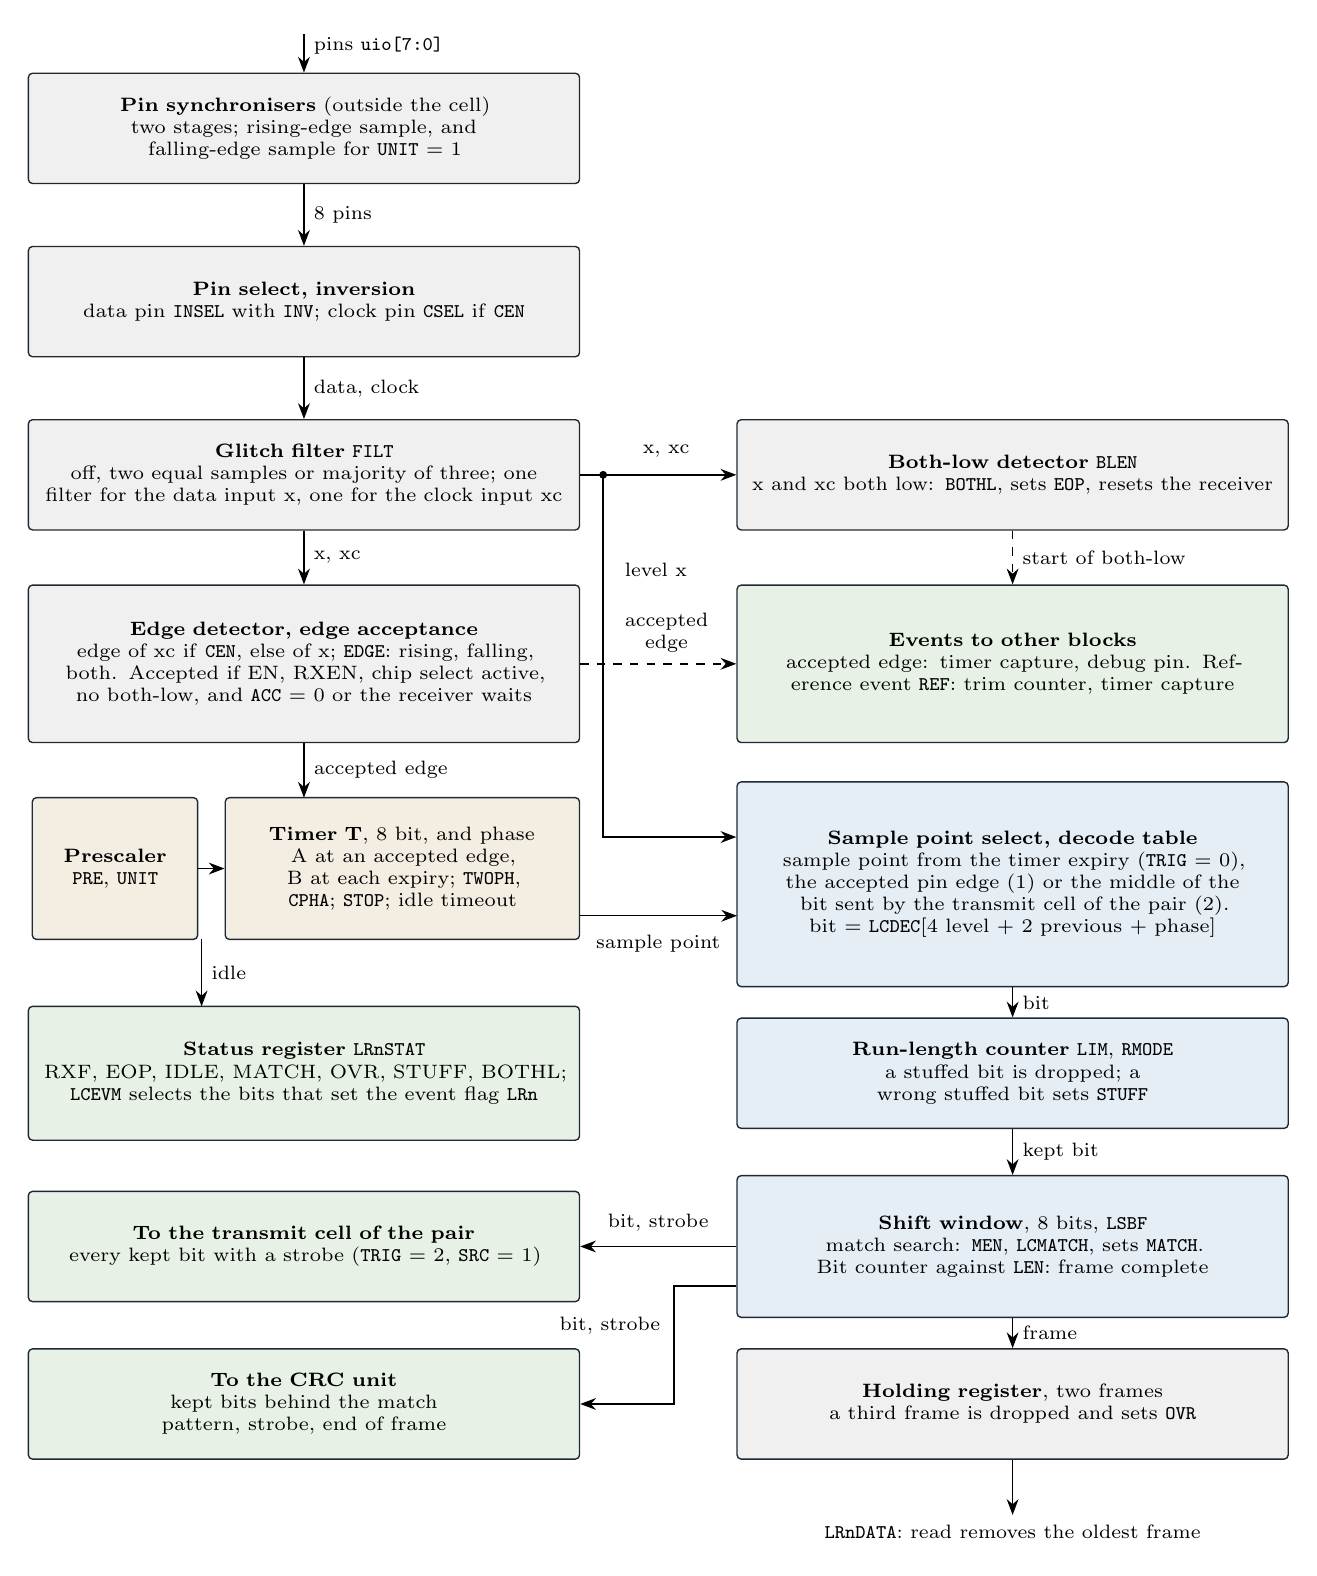
\begin{tikzpicture}[x=1mm,y=1mm,
  b/.style={blk,font=\scriptsize,inner sep=2pt,minimum height=14mm,minimum width=70mm,text width=66mm},
  ev/.style={ar,dashed}]
  % left lane: input path and timing
  \node[b,fill=fillD] (sy) at (35,140) {\textbf{Pin synchronisers} (outside the cell)\\ two stages; rising-edge sample, and falling-edge sample for \reg{UNIT} = 1};
  \node[b,fill=fillD] (ps) at (35,118) {\textbf{Pin select, inversion}\\ data pin \reg{INSEL} with \reg{INV}; clock pin \reg{CSEL} if \reg{CEN}};
  \node[b,fill=fillD] (fl) at (35,96) {\textbf{Glitch filter} \reg{FILT}\\ off, two equal samples or majority of three; one filter for the data input x, one for the clock input xc};
  \node[b,fill=fillD,minimum height=20mm] (ed) at (35,72) {\textbf{Edge detector, edge acceptance}\\ edge of xc if \reg{CEN}, else of x; \reg{EDGE}: rising, falling, both. Accepted if EN, RXEN, chip select active, no both-low, and \reg{ACC} = 0 or the receiver waits};
  \node[b,fill=fillB,minimum width=21mm,text width=18mm,minimum height=18mm] (pre) at (11,46) {\textbf{Prescaler}\\ \reg{PRE}, \reg{UNIT}};
  \node[b,fill=fillB,minimum width=45mm,text width=42mm,minimum height=18mm] (tm) at (47.5,46) {\textbf{Timer T}, 8 bit, and phase\\ A at an accepted edge, B at each expiry; \reg{TWOPH}, \reg{CPHA}; \reg{STOP}; idle timeout};
  \node[b,fill=fillC,minimum height=17mm] (st) at (35,20) {\textbf{Status register} \reg{LRnSTAT}\\ RXF, EOP, IDLE, MATCH, OVR, STUFF, BOTHL; \reg{LCEVM} selects the bits that set the event flag \reg{LRn}};
  \node[b,fill=fillC] (pl) at (35,-2) {\textbf{To the transmit cell of the pair}\\ every kept bit with a strobe (\reg{TRIG} = 2, \reg{SRC} = 1)};
  \node[b,fill=fillC] (cr) at (35,-22) {\textbf{To the CRC unit}\\ kept bits behind the match pattern, strobe, end of frame};
  % right lane: decoding
  \node[b,fill=fillD] (bl) at (125,96) {\textbf{Both-low detector} \reg{BLEN}\\ x and xc both low: \reg{BOTHL}, sets \reg{EOP}, resets the receiver};
  \node[b,fill=fillC,minimum height=20mm] (o1) at (125,72) {\textbf{Events to other blocks}\\ accepted edge: timer capture, debug pin. Reference event \reg{REF}: trim counter, timer capture};
  \node[b,fill=fillA,minimum height=26mm] (dc) at (125,44) {\textbf{Sample point select, decode table}\\ sample point from the timer expiry (\reg{TRIG} = 0), the accepted pin edge (1) or the middle of the bit sent by the transmit cell of the pair (2).\\ bit = \reg{LCDEC}[4 level + 2 previous + phase]};
  \node[b,fill=fillA] (rl) at (125,20) {\textbf{Run-length counter} \reg{LIM}, \reg{RMODE}\\ a stuffed bit is dropped; a wrong stuffed bit sets \reg{STUFF}};
  \node[b,fill=fillA,minimum height=18mm] (sh) at (125,-2) {\textbf{Shift window}, 8 bits, \reg{LSBF}\\ match search: \reg{MEN}, \reg{LCMATCH}, sets \reg{MATCH}. Bit counter against \reg{LEN}: frame complete};
  \node[b,fill=fillD] (hr) at (125,-22) {\textbf{Holding register}, two frames\\ a third frame is dropped and sets \reg{OVR}};
  % arrows, left lane
  \draw[ar] (35,152) -- (sy.north) node[pos=0.3,right,lbl]{pins \texttt{uio[7:0]}};
  \draw[ar] (sy) -- (ps) node[midway,right,lbl]{8 pins};
  \draw[ar] (ps) -- (fl) node[midway,right,lbl]{data, clock};
  \draw[ar] (fl) -- (ed) node[midway,right,lbl]{x, xc};
  \draw[ar] (35,62) -- (35,55) node[pos=0.5,right,lbl]{accepted edge};
  \draw[ar] (pre) -- (tm) node[midway,above,lbl]{};
  \draw[ar] (22,37) -- (22,28.5) node[midway,right,lbl]{idle};
  % cross links
  \draw[ar] (fl.east) -- (bl.west);
  \node[lbl] at (81,99) {x, xc};
  \draw[ar] (73,96) -- (73,50) -- ($(dc.west)+(0,6)$);
  \fill (73,96) circle (0.5);
  \node[lbl,anchor=west] at (74.5,84) {level x};
  \draw[ev] (ed.east) -- (o1.west);
  \node[lbl,anchor=west] at (74.5,76) {accepted\\ edge};
  \draw[ev] (bl.south) -- (o1.north) node[midway,right,lbl]{start of both-low};
  \draw[ar] (70,40) -- (90,40);
  \node[lbl] at (80,36.5) {sample point};
  % arrows, right lane
  \draw[ar] (dc) -- (rl) node[midway,right,lbl]{bit};
  \draw[ar] (rl) -- (sh) node[midway,right,lbl]{kept bit};
  \draw[ar] (sh.south) -- (hr.north) node[midway,right,lbl]{frame};
  \draw[ar] (sh.west) -- (pl.east);
  \node[lbl] at (80,1) {bit, strobe};
  \draw[ar] ($(sh.west)+(0,-5)$) -| (82,-22) -- (cr.east);
  \node[lbl,anchor=east] at (81.5,-12) {bit, strobe};
  \draw[ar] (hr.south) -- ++(0,-7) node[below,lbl]{\reg{LRnDATA}: read removes the oldest frame};
\end{tikzpicture}
}
\caption{Receive cell. The left column is the timing and input path, the right column the decode and data path.
The rules are in section~\ref{sec:lcbeh}. The pin synchronisers are outside the cell. The diagram is drawn
from the intended behaviour and the RTL.}
\label{fig:rx}
\end{figure}

\begin{figure}[!htb]
\centering
\resizebox{\textwidth}{!}{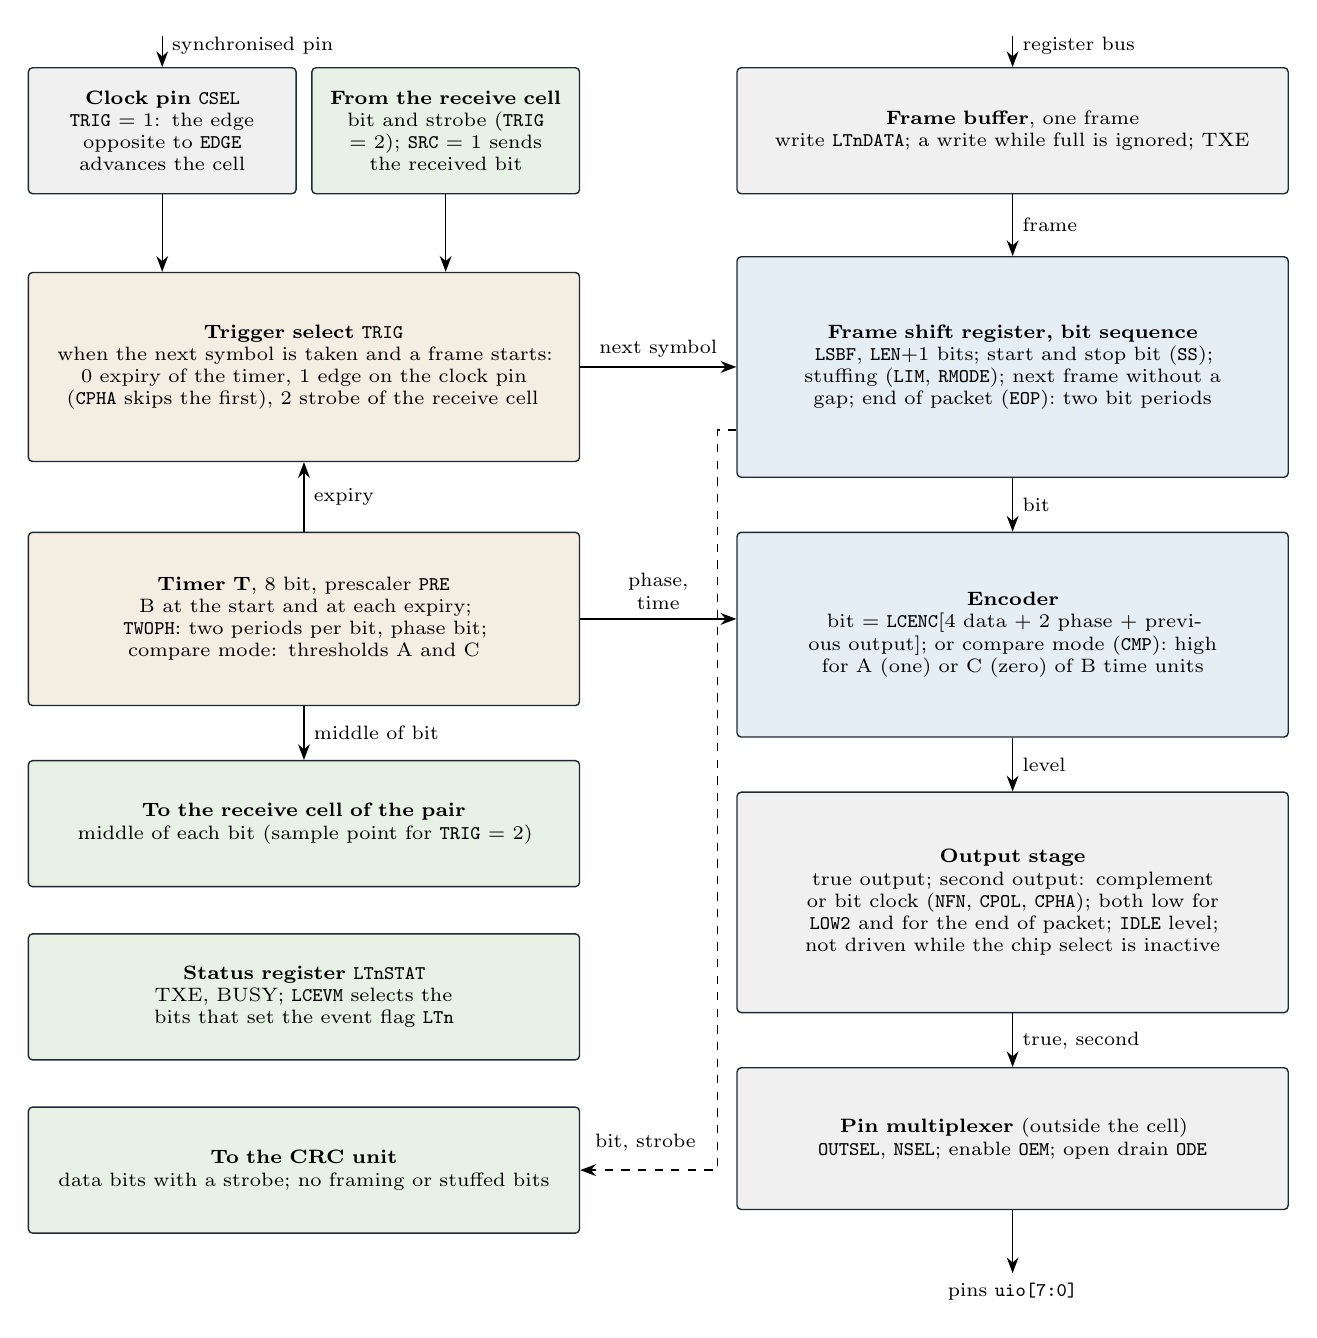
\begin{tikzpicture}[x=1mm,y=1mm,
  b/.style={blk,font=\scriptsize,inner sep=2pt,minimum height=14mm,minimum width=70mm,text width=66mm},
  ev/.style={ar,dashed}]
  % left lane: trigger and timing
  \node[b,fill=fillD,minimum width=34mm,text width=31mm,minimum height=16mm] (cp) at (17,150) {\textbf{Clock pin} \reg{CSEL}\\ \reg{TRIG} = 1: the edge opposite to \reg{EDGE} advances the cell};
  \node[b,fill=fillC,minimum width=34mm,text width=31mm,minimum height=16mm] (rc) at (53,150) {\textbf{From the receive cell}\\ bit and strobe (\reg{TRIG} = 2); \reg{SRC} = 1 sends the received bit};
  \node[b,fill=fillB,minimum height=24mm] (tr) at (35,120) {\textbf{Trigger select} \reg{TRIG}\\ when the next symbol is taken and a frame starts: 0 expiry of the timer, 1 edge on the clock pin (\reg{CPHA} skips the first), 2 strobe of the receive cell};
  \node[b,fill=fillB,minimum height=22mm] (tm) at (35,88) {\textbf{Timer T}, 8 bit, prescaler \reg{PRE}\\ B at the start and at each expiry; \reg{TWOPH}: two periods per bit, phase bit; compare mode: thresholds A and C};
  \node[b,fill=fillC,minimum height=16mm] (tmid) at (35,62) {\textbf{To the receive cell of the pair}\\ middle of each bit (sample point for \reg{TRIG} = 2)};
  \node[b,fill=fillC,minimum height=16mm] (stat) at (35,40) {\textbf{Status register} \reg{LTnSTAT}\\ TXE, BUSY; \reg{LCEVM} selects the bits that set the event flag \reg{LTn}};
  \node[b,fill=fillC,minimum height=16mm] (crc) at (35,18) {\textbf{To the CRC unit}\\ data bits with a strobe; no framing or stuffed bits};
  % right lane: data path
  \node[b,fill=fillD,minimum height=16mm] (fb) at (125,150) {\textbf{Frame buffer}, one frame\\ write \reg{LTnDATA}; a write while full is ignored; TXE};
  \node[b,fill=fillA,minimum height=28mm] (sq) at (125,120) {\textbf{Frame shift register, bit sequence}\\ \reg{LSBF}, \reg{LEN}+1 bits; start and stop bit (\reg{SS}); stuffing (\reg{LIM}, \reg{RMODE}); next frame without a gap; end of packet (\reg{EOP}): two bit periods};
  \node[b,fill=fillA,minimum height=26mm] (en) at (125,86) {\textbf{Encoder}\\ bit = \reg{LCENC}[4 data + 2 phase + previous output]; or compare mode (\reg{CMP}): high for A (one) or C (zero) of B time units};
  \node[b,fill=fillD,minimum height=28mm] (os) at (125,52) {\textbf{Output stage}\\ true output; second output: complement or bit clock (\reg{NFN}, \reg{CPOL}, \reg{CPHA}); both low for \reg{LOW2} and for the end of packet; \reg{IDLE} level; not driven while the chip select is inactive};
  \node[b,fill=fillD,minimum height=18mm] (pm) at (125,22) {\textbf{Pin multiplexer} (outside the cell)\\ \reg{OUTSEL}, \reg{NSEL}; enable \reg{OEM}; open drain \reg{ODE}};
  % arrows
  \draw[ar] (17,162) -- (cp.north) node[pos=0.3,right,lbl]{synchronised pin};
  \draw[ar] (cp.south) -- (cp.south |- tr.north);
  \draw[ar] (rc.south) -- (rc.south |- tr.north);
  \draw[ar] (tm.north) -- (tm.north |- tr.south) node[pos=0.5,right,lbl]{expiry};
  \draw[ar] (tr.east) -- (sq.west |- tr.east) node[pos=0.5,above,lbl]{next symbol};
  \draw[ar] (tm.east) -- (en.west |- tm.east) node[pos=0.5,above,lbl,align=center]{phase,\\ time};
  \draw[ar] (tm.south) -- (tmid.north) node[midway,right,lbl]{middle of bit};
  \draw[ar] (fb) -- (sq) node[midway,right,lbl]{frame};
  \draw[ar] (sq) -- (en) node[midway,right,lbl]{bit};
  \draw[ar] (en) -- (os) node[midway,right,lbl]{level};
  \draw[ar] (os) -- (pm) node[midway,right,lbl]{true, second};
  \draw[ar] (pm.south) -- ++(0,-8) node[below,lbl]{pins \texttt{uio[7:0]}};
  \draw[ar] (125,162) -- (fb.north) node[pos=0.3,right,lbl]{register bus};
  \draw[ev] ($(sq.west)+(0,-8)$) -| (87.5,18) -- (crc.east);
  \node[lbl,anchor=east] at (86,21.5) {bit, strobe};
\end{tikzpicture}
}
\caption{Transmit cell. The dashed line is the strobe and data output to the CRC unit; the cell's middle-of-bit
strobe goes to the receive cell of the pair. The diagram is drawn from the intended behaviour and the RTL.}
\label{fig:tx}
\end{figure}

Receive cell:
\begin{itemize}
\item \textbf{Pin select.} Input from one of the eight bidirectional pins.
\item \textbf{Glitch filter.} Two equal samples or majority of three; can be bypassed.
\item \textbf{Timer} with two reload values. A is loaded on an accepted edge, B on expiry. A prescaler divides
the time unit.
\item \textbf{Edge rule.} Rising, falling or both; accepted always, or only while the cell is waiting.
\item \textbf{Expiry rule.} Reload B and continue, or stop and wait for the next edge. While waiting, B runs as a
timeout and sets the idle flag.
\item \textbf{Decode LUT3} on (pin level, previous sample, phase). It selects level, inverted or NRZI decoding
without a fixed list of modes.
\item \textbf{Shift register} with selectable bit order and a frame length of 1 to 8 bits, and a holding register
for two frames.
\item \textbf{Match register.} After a receiver reset the cell searches for this pattern and delivers no frame
until it is found. The bit after the pattern starts the first frame. This aligns bytes on the Ethernet
start-of-frame delimiter or the USB sync pattern.
\item \textbf{Run-length counter} with programmable limit, counting either ones or equal bits. It drops the
stuffed bit (USB after six ones, CAN after five equal bits).
\item \textbf{Clock pin.} The edge detector can use a second pin, for protocols with a separate clock line.
\item \textbf{Both-low detector.} A status bit shows that the input pin and the second pin are both low, which is
the USB end of packet and frame mark.
\item \textbf{Reference event.} The cell can pass a selected event to the trim counter as a clock reference
(section~\ref{sec:clock}).
\item \textbf{Time unit.} The peripheral clock (section~\ref{sec:clock}), or both edges of the source clock.
\end{itemize}

Transmit cell:
\begin{itemize}
\item \textbf{Frame buffer} for one frame, and the frame being sent.
\item \textbf{Bit sequence.} Bit order, frame length, optional start and stop bit, and bit stuffing by a run-length
counter.
\item \textbf{Timer} for the bit period B. In compare mode A and C are the two high times.
\item \textbf{Encode LUT3} on (data bit, phase, previous output), or compare mode for pulse-width codes.
\item \textbf{Output stage.} True output, a second output that carries either the complement or the bit clock,
a state with both pins low, and an output enable that follows the busy state.
\item \textbf{Clock pin.} The cell can advance on the edges of a pin instead of its timer.
\end{itemize}

Both:
\begin{itemize}
\item \textbf{Chip select pin.} For slave operation a pin frames the transfer: while it is inactive, the cell is
held in reset and does not drive its outputs.
\item \textbf{Links within the pair.} The transmit cell can send one bit for each bit the receive cell delivers,
with its own timing and line code. Together they form a bit-level repeater or line-code converter without
firmware in the data path. The receive cell can take its sample point from the middle of each transmitted bit;
this is the SPI master.
\item \textbf{Configuration registers} are written through a gated clock, one gate per register, because the
flip-flops of the library have no enable input.
\end{itemize}

\begin{table}[H]
\centering\small
\begin{tabular}{@{}lrrr@{}}
\toprule
Cell & IHP cells & Cell area & Flip-flops \\
\midrule
Receive cell & 1\,012 & 15\,900\,$\mu$m$^2$ & 156 \\
Transmit cell & 624 & 11\,400\,$\mu$m$^2$ & 126 \\
Two pairs & 3\,272 & 54\,600\,$\mu$m$^2$ & 564 \\
\bottomrule
\end{tabular}
\caption{Size of the cells (yosys, slow corner library, no timing-driven sizing). The values predate the stored \reg{EOP} status bit and \reg{LCRUN.EOP}, which add about two flip-flops to each cell. The combined cell of the
first version had 1\,668 cells and 24\,700\,$\mu$m$^2$, four of them 99\,000\,$\mu$m$^2$.}
\end{table}

For 10BASE-T at 60\,MHz the input must be sampled on both clock edges, which gives 12 samples per bit. Both
receive cells can do this.

\subsection{Configurations}

\begin{table}[H]
\centering\small
\begin{tabularx}{\linewidth}{@{}l>{\raggedright\arraybackslash}p{34mm}>{\raggedright\arraybackslash}p{30mm}L@{}}
\toprule
Use & Edge rule & A / B & Decode or encode \\
\midrule
UART receive & falling, when idle & 1.5 bit / 1 bit & level \\
USB low-speed receive & both, always & 0.5 bit / 1 bit & NRZI, drop a bit after six ones \\
10BASE-T receive & both, when waiting & 0.75 bit / timeout & inverted level, stop after each sample \\
WS2812 receive, 1-Wire, IR & rising, when waiting & about 0.5 bit / timeout & level \\
SPI & external clock edge, or the transmit cell's timing & none / half period & level; master: the receive cell samples in the middle of each transmitted bit \\
Manchester transmit & none & half bit & data XOR phase, complementary pair \\
USB low-speed transmit & none & 1 bit & NRZI, insert a bit after six ones \\
WS2812 transmit & none & high time / bit period & compare mode, second high time in C \\
\bottomrule
\end{tabularx}
\caption{Configurations for the protocols in scope. The first five rows are receive cells, the last three transmit cells; SPI uses both cells of a pair.}
\end{table}

\textbf{Settings in the firmware.} Table~\ref{tab:cfgfw} gives the register values written by the example firmware
(\texttt{fw/rpe.h} and the programs for each protocol), in the order of the configuration page. All values are
hexadecimal, A, B and C are decimal. Dashes are zero. Values with a pin number $p$ or $q$ depend on the board.
\texttt{HB} is half of the clock period in time units.

\begin{table}[H]
\centering\scriptsize
\setlength{\tabcolsep}{2.5pt}
\resizebox{\textwidth}{!}{%
\begin{tabular}{@{}lccccccccccccc@{}}
\toprule
Use & CTRL & PIN & OUT & CLK & TIM & A & B & C & LUT & SH & MATCH & RUN & EVM \\
\midrule
SPI master, T & A0 & 01 & 13 & 08 & 04 & 1 & HB & 1 & enc F0 & E0 & -- & -- & -- \\
SPI master, R & C0 & 40 & -- & -- & 02 & 1 & 1 & 0 & dec F0 & E0 & -- & -- & 80 \\
SPI slave, T & A0 & 01 & 50 & 20 & 41 & 1 & 1 & 1 & enc F0 & E0 & -- & -- & -- \\
SPI slave, R & C0 & -- & -- & 30 & 41 & 1 & 1 & 0 & dec F0 & E0 & -- & -- & 80 \\
I2C slave, R & C0 & 80 & -- & B0 & 41 & 1 & 1 & 0 & dec F0 & E0 & -- & -- & 80 \\
I2C slave, T & 80 & 02 & 80 & A0 & 41 & 1 & 1 & 1 & enc F0 & E0 & -- & 04 & -- \\
WS2812 control, T & A0 & 01 & 10 & -- & -- & 48 & 75 & 24 & enc F0 & E4 & -- & -- & 40 \\
WS2812 LED, R & C0 & -- & -- & -- & 68 & 36 & 150 & 0 & dec F0 & E0 & -- & -- & 90 \\
WS2812 forward, T & 80 & 01 & 30 & -- & 02 & 48 & 70 & 24 & enc F0 & EC & -- & -- & -- \\
USB, R & C0 & $p$ & -- & $q$|01 & C0 & 20 & 40 & 0 & dec C3 & F2 & 80 & C2 & A0 \\
USB, T & A0 & 02 & $p,q$ & -- & -- & 1 & 40 & 1 & enc A5 & F0 & -- & C2 & 40 \\
\bottomrule
\end{tabular}}
\caption{Cell settings of the example firmware. T: transmit cell, R: receive cell. USB values are for 60\,MHz
(40 cycles per bit); \texttt{PIN} of USB receive is the pin number in bits 7:5, \texttt{CLK} holds the pin of the
second line in bits 7:5 and \reg{BLEN} in bit 0. \texttt{OUT} of USB transmit holds both output pins with \reg{OUTEN} and \reg{NEN}.
\texttt{TIM} combines the edge rule, \reg{ACC}, \reg{STOP}, \reg{TWOPH} and \reg{TRIG} as in table~\ref{tab:fields}.}
\label{tab:cfgfw}
\end{table}

UART and 10BASE-T are set up from a mix of fixed values and values computed from the baud rate or the unit, so
only the fields that decide the behaviour are listed. UART transmit: \reg{OEM} = 1, \reg{LCENC} = level,
\reg{LEN} = 7, \reg{LSBF}, \reg{SS}, \reg{IDLE} = 1. UART receive: \reg{EDGE} = falling, \reg{ACC} = 1,
\reg{STOP} = 2, A = 1.5 bit, B = 1 bit, \reg{LCDEC} = level, \reg{LEN} = 7, \reg{LSBF}. 10BASE-T receive:
\reg{EDGE} = both, \reg{ACC} = 1, \reg{STOP} = 1, A = 9, B = 24, \reg{LCDEC} = 0F, or F0 with \reg{INV}, \reg{LEN} = 7, \reg{MEN}, match D5,
event mask \reg{RXF} and \reg{IDLE}, \reg{UNIT} = 1. 10BASE-T transmit: \reg{TWOPH}, B = 3, Manchester encode table,
\reg{LEN} = 7.

\subsection{Register set}\label{sec:lcreg}

This subsection describes the registers and their fields. Addresses and bit positions are in
section~\ref{sec:map}.

\textbf{Access.} A receive cell has 14 configuration registers, a transmit cell 14, in the configuration page.
Each cell has a status and a data register on the fast I/O tier. All four cells are at fixed addresses. Each
pair has an owner core; only the owner can access the cells of the pair and sees their event flags
(section~\ref{sec:bus}). Both cell types use the same register names and offsets. R marks a register or field
of the receive cell, T of the transmit cell.

\begin{table}[H]
\centering\small
\begin{tabularx}{\linewidth}{@{}lllL@{}}
\toprule
Register & Cell & Mapping & Content \\
\midrule
\reg{LCCTRL} & R, T & page & \reg{EN}, \reg{PRE[2:0]}; R: \reg{RXEN}, \reg{UNIT}; T: \reg{TXEN} \\
\reg{LCPIN} & R, T & page & R: \reg{INSEL[2:0]}, \reg{INV}, \reg{FILT[1:0]}; T: \reg{OEM[1:0]} \\
\reg{LCOUT} & T & page & \reg{OUTSEL[2:0]}, \reg{OUTEN}, \reg{NSEL[2:0]}, \reg{NEN} \\
\reg{LCCLK} & R, T & page & \reg{CSEL[2:0]}, \reg{CPHA}; R: \reg{CEN}, \reg{BLEN}; T: \reg{NFN}, \reg{CPOL} \\
\reg{LCTIM} & R, T & page & \reg{EDGE[1:0]}, \reg{TWOPH}, \reg{TRIG[1:0]}; R: \reg{ACC}, \reg{STOP[1:0]} \\
\reg{LCA} & R, T & page & R: timer reload on an accepted edge. T: high time for a one in compare mode \\
\reg{LCB} & R, T & page & R: timer reload on expiry. T: bit or half-bit period \\
\reg{LCC} & T & page & High time for a zero in compare mode \\
\reg{LCDEC} & R & page & Decode lookup table, 8 bits \\
\reg{LCENC} & T & page & Encode lookup table, 8 bits \\
\reg{LCSH} & R, T & page & \reg{LEN[2:0]}, \reg{LSBF}; R: \reg{MEN}; T: \reg{SRC}, \reg{CMP}, \reg{SS} \\
\reg{LCMATCH} & R & page & Match pattern, 8 bits \\
\reg{LCRUN} & R, T & page & \reg{LIM[2:0]}, \reg{RMODE}; R: \reg{REF[1:0]}; T: \reg{LOW2}, \reg{IDLE}, \reg{EOP} \\
\reg{LCEVM} & R, T & page & Event mask over the bits of the cell's status register \\
\reg{LCCS} & R, T & page & \reg{SSEL[2:0]}, \reg{SSEN}, \reg{SSPOL} \\
\reg{LCEC} & R & page & \reg{EC[3:0]}: edge count (section~\ref{sec:lcx}) \\
\reg{LCX} & R, T & page & \reg{PAR[1:0]}, \reg{X9}; R: \reg{BCD}, \reg{BEV}, \reg{STP}, \reg{STA}, \reg{ECF}; T: \reg{ESTR} (section~\ref{sec:lcx}) \\
\reg{LRnSTAT} & R & fast & \reg{RXF}, \reg{FERR}, \reg{EOP}, \reg{IDLE}, \reg{MATCH}, \reg{OVR}, \reg{STUFF}, \reg{BOTHL}; write 1 to clear the latched bits \\
\reg{LRnDATA} & R & fast & Read: oldest received frame \\
\reg{LTnSTAT} & T & fast & \reg{TXE}, \reg{BUSY}; read only \\
\reg{LTnDATA} & T & fast & Write: frame to transmit \\
\bottomrule
\end{tabularx}
\caption{Registers of the line cells. ``Page'' is the configuration page, ``fast'' the fast I/O tier; $n$ is the
number of the pair, 0 or 1.}
\end{table}

\begin{table}[H]
\centering\small
\begin{tabularx}{\linewidth}{@{}llL@{}}
\toprule
Field & Bits & Meaning \\
\midrule
\reg{EN} & 1 & Cell enabled. Clearing it resets timer, bit counter, buffers and status \\
\reg{RXEN}, \reg{TXEN} & 1 + 1 & R: receiver active; while 0 the receiver is reset and the holding register keeps its frames. T: transmitter active; clearing it ends transmission at once \\
\reg{UNIT} & 1 & Time unit: peripheral clock, or both edges of the source clock (half a clock period) \\
\reg{PRE} & 3 & Prescaler for the time unit: 1, 2, 4, \dots, 128 \\
\midrule
\reg{INSEL} & 3 & Input pin, one of the eight bidirectional pins \\
\reg{INV} & 1 & Invert the input \\
\reg{FILT} & 2 & Glitch filter: off, two equal samples, majority of three \\
\reg{OEM} & 2 & Output enable: from the port direction register, always driven, driven while the cell is busy \\
\reg{OUTSEL}, \reg{OUTEN} & 3 + 1 & Pin for the true output, and its enable \\
\reg{NSEL}, \reg{NEN} & 3 + 1 & Pin for the second output, and its enable \\
\reg{NFN} & 1 & Function of the second output: complement of the true output, or bit clock \\
\reg{CSEL}, \reg{CEN} & 3 + 1 & R: separate clock pin for the edge detector, and its enable; without it the edge detector uses the input pin. T: clock pin for \reg{TRIG} = 1 \\
\reg{CPOL}, \reg{CPHA} & 1 + 1 & Idle level of the bit clock, and the clock phase: data is sampled at the first clock edge of a bit (0) or at the second (1) \\
\reg{BLEN} & 1 & Enables the both-low detector on the input pin and pin \reg{CSEL} \\
\midrule
\reg{EDGE} & 2 & Edge that is detected: none, rising, falling, both \\
\reg{ACC} & 1 & Edge accepted always, or only while the cell is waiting \\
\reg{STOP} & 2 & After expiry: keep running, stop after each sample, stop after a complete frame \\
\reg{TWOPH} & 1 & One bit takes two timer periods; the phase input of the lookup tables alternates \\
\reg{TRIG} & 2 & R: sample point from the timer, from an accepted pin edge (external clock), or from the middle of each bit of the transmit cell. T: next bit from the timer, from an edge on the clock pin, or one bit per received bit of the receive cell \\
\reg{LCA} & 8 & Loaded into the timer on an accepted edge. In compare mode: high time for a one \\
\reg{LCB} & 8 & Loaded on expiry: the bit or half-bit period. While waiting: timeout that sets \reg{IDLE} \\
\reg{LCC} & 8 & In compare mode: high time for a zero \\
\midrule
\reg{LEN} & 3 & Frame length minus one: a frame has \reg{LEN}+1 bits, 1 to 8 \\
\reg{LSBF} & 1 & Least significant bit first \\
\reg{SRC} & 1 & Bit source for transmit: own frame buffer, or the receive cell's decoded bit \\
\reg{CMP} & 1 & Transmit in compare mode (pulse width) and not through the encode table \\
\reg{MEN} & 1 & Match enabled: the bit counter resets when the shift register equals \reg{LCMATCH} \\
\reg{SS} & 1 & Transmit adds a start bit at the inverse idle level and a stop bit at the idle level \\
\reg{LIM} & 3 & Run length limit, 0 switches stuffing off \\
\reg{RMODE} & 1 & Count ones, or count equal bits \\
\reg{LOW2} & 1 & Drive both outputs low while set \\
\reg{EOP} & 1 & After the last bit of a frame both outputs are low for two bit periods; \reg{BUSY} stays set during that time. For timer-triggered transmission \\
\reg{IDLE} & 1 & Output level while not transmitting \\
\reg{REF} & 2 & Reference event for the clock loop: none, accepted edge, both pins low, both pins low after the line was idle \\
\reg{SSEL}, \reg{SSEN}, \reg{SSPOL} & 3 + 1 + 1 & Chip select pin for slave operation, its enable and its active level \\
\bottomrule
\end{tabularx}
\caption{Configuration fields.}
\label{tab:fields}
\end{table}

\textbf{Status bits.} A status bit selected in \reg{LCEVM} sets the cell's event flag. Latched bits are cleared by
writing a one to them; if the event happens in the same cycle, the bit stays set. Disabling a cell
(\reg{EN} = 0) clears all status bits and the holding register or frame buffer. A receiver reset (rule R12) does
not clear the latched bits.

\begin{table}[H]
\centering\small
\begin{tabularx}{\linewidth}{@{}lllL>{\raggedright\arraybackslash}p{34mm}@{}}
\toprule
Bit & Cell & Kind & Set when & Cleared by \\
\midrule
\reg{RXF} (7) & R & level & at least one frame is in the holding register & reading \reg{LRnDATA} removes the oldest frame \\
\reg{TXE} (6) & T & level & the frame buffer is empty; it is set again when the frame moves to the shift register & a write to \reg{LTnDATA} that is accepted \\
\reg{EOP} (5) & R & latched & both pins went low (start of both-low, rule S3) & writing 1 \\
\reg{BUSY} (5) & T & level & a frame is being sent, including the end-of-packet periods & the end of the frame \\
\reg{IDLE} (4) & R & latched & the line became idle (rule R13) & writing 1 \\
\reg{MATCH} (3) & R & latched & the match pattern was found (rule R9) & writing 1 \\
\reg{OVR} (2) & R & latched & a completed frame was dropped, because the holding register was full (rule R11) & writing 1 \\
\reg{STUFF} (1) & R & latched & a stuffed bit broke the run-length rule (rules R6, R7) & writing 1 \\
\reg{BOTHL} (0) & R & level & the input pin and the clock pin are both low, with \reg{EN} = 1 & the pins leaving the state \\
\bottomrule
\end{tabularx}
\caption{Status bits. Bit 6 of a receive cell and the bits 7 and 4 to 0 of a transmit cell read as 0. The bits keep the
positions they had in the combined cell.}
\end{table}

\textbf{Lookup tables.} The decode table is indexed by $4\cdot\mathit{pin} + 2\cdot\mathit{previous\ sample} +
\mathit{phase}$, the encode table by $4\cdot\mathit{data} + 2\cdot\mathit{phase} + \mathit{previous\ output}$.
Bit $i$ of the register is the output for index $i$.

\begin{table}[H]
\centering\small
\begin{tabular}{@{}lll@{}}
\toprule
Table & Function & Value \\
\midrule
Decode & level & \texttt{0xF0} \\
Decode & inverted level & \texttt{0x0F} \\
Decode & NRZI, one when the level did not change & \texttt{0xC3} \\
Encode & NRZ & \texttt{0xF0} \\
Encode & NRZI, toggle on zero & \texttt{0xA5} \\
Encode & Manchester, first half inverted data, second half data & \texttt{0xC3} \\
\bottomrule
\end{tabular}
\caption{Lookup table values for common line codes.}
\end{table}

\begin{table}[H]
\centering\small
\begin{tabularx}{\linewidth}{@{}lllllL@{}}
\toprule
Use & Unit, prescaler & \reg{EDGE}, \reg{ACC}, \reg{STOP} & A & B & Other fields \\
\midrule
UART receive, 115\,200 baud & clock, 4 & falling, waiting, frame & 195 & 130 & \reg{LCDEC}=\texttt{0xF0}, \reg{LSBF}, \reg{LEN}=8 \\
USB low-speed receive & clock, 1 & both, always, run & 20 & 40 & \reg{LCDEC}=\texttt{0xC3}, \reg{LIM}=6, count ones, match on the sync pattern \\
10BASE-T receive & both edges, 1 & both, waiting, sample & 9 & 24 & \reg{LCDEC}=\texttt{0x0F}, match on the start-of-frame delimiter \\
WS2812 receive & clock, 1 & rising, waiting, sample & 36 & 150 & \reg{LCDEC}=\texttt{0xF0}, most significant bit first \\
10BASE-T transmit & clock, 1 & none & -- & 3 & \reg{TWOPH}, \reg{LCENC}=\texttt{0xC3}, complementary output \\
USB low-speed transmit & clock, 1 & none & -- & 40 & \reg{LCENC}=\texttt{0xA5}, \reg{LIM}=6, complementary output, \reg{OEM}=busy \\
WS2812 transmit & clock, 1 & none & 48 & 75 & \reg{CMP}, \reg{LCC}=24 \\
\bottomrule
\end{tabularx}
\caption{Example settings at a 60\,MHz clock with the peripheral divider at 1. A and B are in time units after the prescaler.}
\end{table}

The timeout in \reg{LCB} covers at most 255 time units. Longer gaps, such as the WS2812 reset time, are
measured with the core's wake-up time. The UART example does not check the stop bit; firmware can read the pin through the port register for that.

\subsection{CRC and LFSR unit}

One 32-bit shift register with a polynomial register, clocked by a selected cell's bit strobe or fed with
bytes by firmware. It covers the checksums of USB, CAN, Ethernet and 1-Wire, and can serve as a pseudo-random
source. Rules are in section~\ref{sec:perbeh}, size and tests in section~\ref{sec:timver}.

\section{Line cell behaviour}\label{sec:lcbeh}

This section defines the behaviour of the line cells as numbered rules: input path and receiver for the receive cell, transmitter and output stage for the transmit cell. The rules are the reference for the RTL
and for the tests. Section~\ref{sec:lcchk} reports a check of the rules against a behavioural model.

\subsection{Time units}

\begin{enumerate}[label=\textbf{T\arabic*},leftmargin=2.6em]
\item With \reg{UNIT} = 0 the base unit is one cycle of the peripheral clock. The cell's time unit is $2^{\mathtt{PRE}}$
base units.
\item With \reg{UNIT} = 1 the time unit is half a period of the source clock. The input is sampled on both clock
edges, and two time units are processed per clock cycle. \reg{PRE} and the peripheral divider are not applied.
Only the receive cell has this setting. \reg{LCA} and \reg{LCB} must be at least 2, so that there is at most one sample point per clock cycle.
\item Each cell has its own prescaler. It restarts from zero on every accepted edge in a receive cell and at the start of a frame in a transmit cell, so the first
time unit after such an event has full length.
\item A timer value of 0 in \reg{LCA}, \reg{LCB} or \reg{LCC} means 256.
\end{enumerate}

\subsection{Input path}

\begin{enumerate}[label=\textbf{I\arabic*},leftmargin=2.6em]
\item The data input is pin \reg{INSEL} of the bidirectional port, after the port's two-stage synchroniser and
inverted if \reg{INV} is set.
\item The glitch filter works on base units. \reg{FILT} = 1: the output takes a new level when two consecutive
samples agree. \reg{FILT} = 2: the output is the majority of the last three samples. The filter delays the
signal by one or two base units.
\item If \reg{CEN} is set, a second pin \reg{CSEL} passes through an identical synchroniser and filter and is the
clock input. Edges are then detected on the clock input; otherwise on the data input.
\item An edge is \emph{accepted} if the cell is enabled, its direction matches \reg{EDGE}, the chip select is active
or not used, both-low is not active, and either \reg{ACC} = 0 or the receiver is in the waiting state.
\item If \reg{SSEN} is set, pin \reg{SSEL} is the chip select, active at level \reg{SSPOL}. While it is inactive the
receiver and the transmitter are held in their reset state (rule R12) and the cell does not drive its outputs.
\item If \reg{BLEN} is set, \emph{both-low} is active while the data input and pin \reg{CSEL} are both low after
filtering. The status bit \reg{BOTHL} shows it, and its start sets the stored bit \reg{EOP}. The start of both-low resets the receiver (rule R12).
\end{enumerate}

Synchroniser and filter delay the data and the clock input equally. Sample positions relative to the line are
therefore not shifted by them.

\subsection{Receiver}

The receiver is either \emph{waiting} or \emph{running}. Figure~\ref{fig:rxstate} shows the states, and a frame with its sample points and timeout. It has a timer T, a phase bit, the previous sample, a bit
counter, a run-length counter and a window of the last eight decoded bits.

\begin{figure}[!htb]
\centering
\resizebox{\textwidth}{!}{% SPDX-FileCopyrightText: (c) 2026 Tim S. B. (GitHub: cpldcpu)
% SPDX-License-Identifier: Apache-2.0
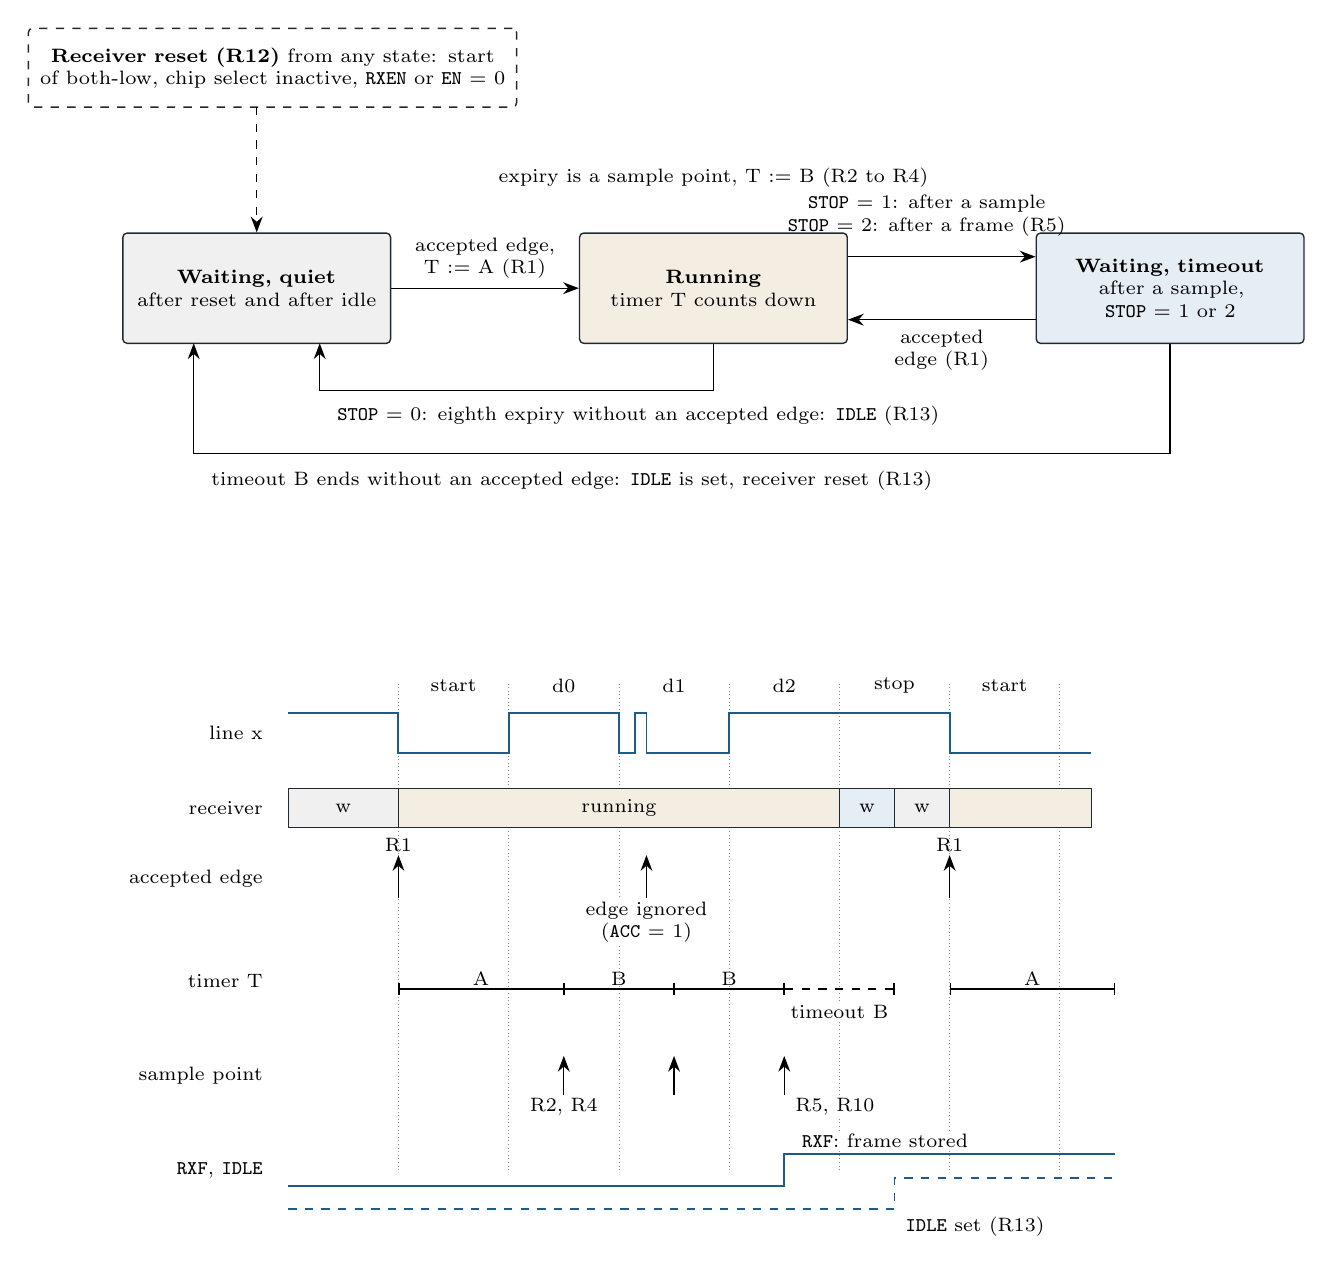
\begin{tikzpicture}[x=1mm,y=1mm,
  sb/.style={blk,font=\scriptsize,inner sep=2pt,minimum height=14mm,minimum width=34mm,text width=31mm}]
  % ---------------- state graph
  \node[sb,fill=fillD] (s0) at (22,112) {\textbf{Waiting, quiet}\\ after reset and after idle};
  \node[sb,fill=fillB] (s1) at (80,112) {\textbf{Running}\\ timer T counts down};
  \node[sb,fill=fillA] (s2) at (138,112) {\textbf{Waiting, timeout}\\ after a sample, \reg{STOP} = 1 or 2};
  \draw[ar] (s0.east) -- (s1.west) node[midway,above,lbl,align=center]{accepted edge,\\ T := A (R1)};
  \draw[ar] ($(s1.east)+(0,4)$) -- ($(s2.west)+(0,4)$) node[pos=0.42,above,lbl,align=center,inner sep=1pt,yshift=2.2mm]{\reg{STOP} = 1: after a sample\\ \reg{STOP} = 2: after a frame (R5)};
  \draw[ar] ($(s2.west)+(0,-4)$) -- ($(s1.east)+(0,-4)$) node[midway,below,lbl,align=center]{accepted\\ edge (R1)};
  \node[lbl,align=center] at (80,126) {expiry is a sample point, T := B (R2 to R4)};
  \draw[ar] (s1.south) -- (80,99) -| (30,105);
  \node[lbl,anchor=west] at (31,95.8) {\reg{STOP} = 0: eighth expiry without an accepted edge: \reg{IDLE} (R13)};
  \draw[ar] (s2.south) -- (138,91) -| (14,105);
  \node[lbl,anchor=west] at (15,87.5) {timeout B ends without an accepted edge: \reg{IDLE} is set, receiver reset (R13)};
  \node[blk,fill=white,font=\scriptsize,inner sep=2pt,minimum width=62mm,text width=59mm,minimum height=10mm,dashed] (rs) at (24,140) {\textbf{Receiver reset (R12)} from any state: start of both-low, chip select inactive, \reg{RXEN} or \reg{EN} = 0};
  \draw[ar,dashed] (22,135) -- (s0.north);
  % ---------------- timing view
  \def\w{14}
  \def\xz{40}
  % bit boundaries
  \foreach \i in {0,...,6} { \draw[densely dotted,line width=0.3pt,black!45] ({\xz+\i*\w},0) -- ({\xz+\i*\w},62); }
  \node[lbl,anchor=east] at (24,55.5) {line x};
  \draw[line width=0.7pt,accent] (26,58) -- (40,58) -- (40,53) -- (54,53) -- (54,58) -- (68,58) -- (68,53) -- (70,53) -- (70,58) -- (71.5,58) -- (71.5,53) -- (82,53) -- (82,58) -- (110,58) -- (110,53) -- (128,53);
  \foreach \i/\t in {0/start,1/d0,2/d1,3/d2,4/stop,5/start} {
    \node[lbl] at ({\xz+\i*\w+\w/2},61.5) {\t};
  }
  \node[lbl,anchor=east] at (24,46) {receiver};
  \fill[fillD,draw=ink,line width=0.4pt] (26,43.5) rectangle (40,48.5);
  \fill[fillB,draw=ink,line width=0.4pt] (40,43.5) rectangle (96,48.5);
  \fill[fillA,draw=ink,line width=0.4pt] (96,43.5) rectangle (103,48.5);
  \fill[fillD,draw=ink,line width=0.4pt] (103,43.5) rectangle (110,48.5);
  \fill[fillB,draw=ink,line width=0.4pt] (110,43.5) rectangle (128,48.5);
  \node[lbl] at (68,46) {running};
  \node[lbl,inner sep=0pt] at (99.5,46) {w};
  \node[lbl,inner sep=0pt] at (33,46) {w};
  \node[lbl,inner sep=0pt] at (106.5,46) {w};
  \node[lbl,anchor=east] at (24,37) {accepted edge};
  \draw[ar] (40,34.5) -- (40,40) node[above,lbl,inner sep=1pt]{R1};
  \draw[ar] (110,34.5) -- (110,40) node[above,lbl,inner sep=1pt]{R1};
  \draw[ar] (71.5,34.5) -- (71.5,40) ;
  \node[lbl,anchor=north,inner sep=1pt,align=center,fill=white] at (71.5,34.5) {edge ignored\\ (\reg{ACC} = 1)};
  \node[lbl,anchor=east] at (24,24) {timer T};
  \draw[|-|,line width=0.4pt] (40,23) -- (61,23); \node[lbl,anchor=south,inner sep=0.6pt] at (50.5,23.2) {A};
  \draw[|-|,line width=0.4pt] (61,23) -- (75,23); \node[lbl,anchor=south,inner sep=0.6pt] at (68,23.2) {B};
  \draw[|-|,line width=0.4pt] (75,23) -- (89,23); \node[lbl,anchor=south,inner sep=0.6pt] at (82,23.2) {B};
  \draw[|-|,dashed,line width=0.4pt] (89,23) -- (103,23); \node[lbl,anchor=north,inner sep=0.6pt,fill=white] at (96,21.2) {timeout B};
  \draw[|-|,line width=0.4pt] (110,23) -- (131,23); \node[lbl,anchor=south,inner sep=0.6pt] at (120.5,23.2) {A};
  \node[lbl,anchor=east] at (24,12) {sample point};
  \foreach \x in {61,75,89} { \draw[ar] (\x,9.5) -- (\x,14.5); }
  \node[lbl,anchor=north,inner sep=1pt] at (61,9.5) {R2, R4};
  \node[lbl,anchor=north west,inner sep=1pt,fill=white] at (90,9.5) {R5, R10};
  \node[lbl,anchor=east] at (24,0) {\reg{RXF}, \reg{IDLE}};
  \draw[line width=0.7pt,accent] (26,-2) -- (89,-2) -- (89,2) -- (131,2);
  \node[lbl,anchor=south west,inner sep=0.6pt,fill=white] at (91,2.6) {\reg{RXF}: frame stored};
  \draw[line width=0.7pt,accent,dashed] (26,-5) -- (103,-5) -- (103,-1) -- (131,-1);
  \node[lbl,anchor=north west,inner sep=1pt] at (104,-5.5) {\reg{IDLE} set (R13)};
\end{tikzpicture}
}
\caption{Top: states of the receiver and the rules that change them. ``Waiting, quiet'' is the state after a reset
and after the idle condition; the transitions are the same as from ``waiting, timeout'' except that no timeout
runs. Bottom: a UART-like frame with \reg{STOP} = 2, A = 1.5 bit, B = 1 bit, one edge ignored because
\reg{ACC} = 1, and the timeout ending in the stop bit. The timing is drawn from the rules, not from simulation.}
\label{fig:rxstate}
\end{figure}

\begin{enumerate}[label=\textbf{R\arabic*},leftmargin=2.6em]
\item \textbf{Accepted edge.} T is loaded with A, the phase bit is cleared and the receiver is running. If the
receiver was waiting, the previous sample is set to the input level before the edge.
\item \textbf{Running.} T is decremented once per time unit, except in the unit of an accepted edge. When it
reaches zero, this is an \emph{expiry}. An expiry therefore occurs A time units after an accepted edge, and the
input level sampled at it lies between A and A+1 time units after the edge on the line.
\item \textbf{Phase.} With \reg{TWOPH} = 0 every expiry is a sample point and the phase input of the decode table is
0. With \reg{TWOPH} = 1 the phase bit toggles at each expiry. The expiry that ends phase 0 is the leading one. The
sample point is the leading expiry if \reg{CPHA} = 0 and the trailing expiry if \reg{CPHA} = 1.
\item \textbf{Decoding.} At a sample point the decoded bit is bit $4\cdot\mathit{level} + 2\cdot\mathit{previous} +
\mathit{phase}$ of \reg{LCDEC}, with the phase value before it toggles. The previous sample is then set to the
level.
\item \textbf{After an expiry.} \reg{STOP} = 0: T is loaded with B. \reg{STOP} = 1: after a sample point the receiver
waits. \reg{STOP} = 2: the receiver waits after the sample that completes a frame; otherwise T is loaded with B.
\item \textbf{Stuffing, counting ones} (\reg{RMODE} = 0, \reg{LIM} $>$ 0). A counter holds the number of consecutive
decoded ones. When it reaches \reg{LIM}, the next decoded bit is a stuffed bit. It is discarded, and the counter
is cleared. If the stuffed bit is a one, \reg{STUFF} is set.
\item \textbf{Stuffing, counting equal bits} (\reg{RMODE} = 1). The counter holds the length of the current run of
equal bits. When it reaches \reg{LIM}, the next decoded bit is a stuffed bit. It is discarded, and it starts a
new run of length 1. If it equals the bit before it, \reg{STUFF} is set. The counter stops at 7. \reg{LIM} = 1 together with \reg{RMODE} = 1 is not meaningful.
\item \textbf{Shifting.} Every decoded bit that is not discarded enters the window and increments the bit counter.
It is also passed with a strobe to the transmit cell of the pair. The CRC unit gets the same bit and strobe only
once the match pattern has been found (or at once if \reg{MEN} = 0), and gets a frame strobe when a frame is
complete. Bits before the match are therefore not seen by the CRC unit.
\item \textbf{Search for the match pattern.} If \reg{MEN} is set, the receiver searches after each reset (rule R12).
While it searches, no frame is delivered. When at least eight bits have been received since the reset and the window equals \reg{LCMATCH}, read in the order given by \reg{LSBF}, the search ends, \reg{MATCH} is set and the bit counter is cleared. The pattern itself is not
delivered. The search starts again only at the next receiver reset.
\item \textbf{Frame.} When the bit counter reaches \reg{LEN}+1, the last \reg{LEN}+1 bits form a frame and the bit
counter is cleared. With \reg{LSBF} = 1 the first received bit is bit 0 of the frame; otherwise it is bit
\reg{LEN}. Unused upper bits are zero.
\item \textbf{Holding register.} It holds two frames. A completed frame is stored if there is room; otherwise it is
dropped and \reg{OVR} is set. \reg{RXF} is set while at least one frame is stored. Reading \reg{LRnDATA} returns the oldest frame and removes it.
\item \textbf{Receiver reset.} The bit counter and the run-length counter are cleared, an incomplete frame is
discarded, the search of rule R9 starts again, and the receiver waits. Frames already in the holding register
are kept. The receiver is reset by the idle condition (rule R13), the start of both-low, an inactive chip
select, and clearing \reg{RXEN} or \reg{EN}.
\item \textbf{Idle.} With \reg{STOP} = 1 or 2: when the receiver starts to wait, a timeout of B time units starts.
If it ends before an edge is accepted, the line is idle. With \reg{STOP} = 0: the line is idle at the eighth
consecutive expiry without an accepted edge; no sample is taken at that expiry. When the line becomes idle,
\reg{IDLE} is set and the receiver is reset. The line stays idle until the next accepted edge.
\end{enumerate}

\subsection{Transmitter}

The transmit cell has a one-frame buffer, the frame being sent, a run-length counter and its own timer T.

\begin{enumerate}[label=\textbf{X\arabic*},leftmargin=2.6em]
\item \textbf{Buffer.} Writing \reg{LTnDATA} stores a frame in the buffer and clears \reg{TXE}. A write while
\reg{TXE} is 0 is ignored.
\item \textbf{Start.} If \reg{TXEN} is set, the transmitter is not busy and the buffer is full, the frame moves to
the shift register, \reg{TXE} and \reg{BUSY} are set, the run-length counter and the phase bit are cleared, T
is loaded with B, and the first bit is encoded in the same time unit.
\item \textbf{Bit order and framing.} Bits are sent in the order given by \reg{LSBF}, \reg{LEN}+1 per frame. With
\reg{SS} set, a start bit with the inverse of \reg{IDLE} precedes them and a stop bit with the value of
\reg{IDLE} follows. Start and stop bits are not counted for stuffing.
\item \textbf{Bit time.} With \reg{TWOPH} = 0 a bit lasts B time units. With \reg{TWOPH} = 1 it lasts two periods of B;
the phase bit is 0 in the first and 1 in the second.
\item \textbf{Encoding.} At the start of each period the true output is bit $4\cdot\mathit{data} + 2\cdot\mathit{phase} +
\mathit{previous\ output}$ of \reg{LCENC}. Before the first bit of a frame the previous output is the level the
output had while idle.
\item \textbf{Compare mode} (\reg{CMP} = 1, \reg{TWOPH} = 0). The true output is high from the start of the bit for A
time units if the data bit is one, and for C time units if it is zero, and low for the rest of the bit.
\item \textbf{Stuffing.} The run-length counter follows the transmitted data bits by the same rules as in the
receiver. When it reaches \reg{LIM}, a stuffed bit is sent before the next data bit: a zero for \reg{RMODE} = 0, the
inverse of the last bit for \reg{RMODE} = 1.
\item \textbf{End of a frame.} If the buffer is full, the next frame starts without a gap, and the run-length
counter continues. Otherwise \reg{BUSY} is cleared and the outputs take their idle levels. With \reg{LCRUN.EOP} = 1
(\reg{TRIG} = 0 only) the transmitter first holds both outputs low for two bit periods after the last bit,
\reg{BUSY} stays set during them, and a frame in the buffer starts after them.
\item \textbf{Bit clock.} While busy, the bit clock is \reg{CPOL} exclusive-or the phase bit exclusive-or \reg{CPHA}; otherwise it is \reg{CPOL}. With \reg{CPHA} = 0 the first clock edge is in the middle of the bit, with \reg{CPHA} = 1 at its start.
\item \textbf{Middle of the bit.} The transmit cell gives a strobe at the expiry in the middle of each bit with
\reg{TWOPH} = 1, and at every expiry otherwise. A receive cell with \reg{TRIG} = 2 takes it as its sample
point and does not use rules R1, R2 and R13. The input must be valid in the middle of the bit: the delay from
the clock output through the other device and back through the synchroniser has to be shorter than half a bit.
\end{enumerate}

\subsection{Other shift triggers}

\begin{enumerate}[label=\textbf{G\arabic*},leftmargin=2.6em]
\item \textbf{Pin edge} (\reg{TRIG} = 1). The timer is not used. In both cells \reg{EDGE} names the clock edge that
samples. In the receive cell an accepted edge is a sample point. The transmit cell starts when the buffer is
full and the chip select is active, or none is used, and outputs its first bit at once. It advances to the next
bit at each edge of the opposite direction on pin \reg{CSEL}. With \reg{CPHA} = 1 it ignores the first such
edge after its start, as the first bit is already on the pin. In that mode no edge follows the last bit, and
\reg{BUSY} stays set until the chip select is released. The frame buffer keeps its frame while the chip select
is inactive.
\item \textbf{One bit per received bit} (transmit cell, \reg{TRIG} = 2). Each strobe of rule R8 from the receive cell
of the pair starts one bit time of the transmitter. With \reg{SRC} = 1 the data bit is the received bit, and
the frame buffer is not used. The bit time B must be shorter than the bit period of the received signal.
\end{enumerate}

\subsection{Output stage}

\begin{table}[H]
\centering\small
\begin{tabular}{@{}>{\raggedright\arraybackslash}p{72mm}ll@{}}
\toprule
Condition, in order of priority & True output & Second output \\
\midrule
\reg{EN} = 0 & pins not used by the cell & pins not used by the cell \\
Chip select inactive & not driven & not driven \\
\reg{LOW2} = 1, or in the two bit periods after a frame with \reg{LCRUN.EOP} = 1 & low & low \\
Busy, \reg{NFN} = 0 & encoded level & inverse of the true output \\
Busy, \reg{NFN} = 1 & encoded level & bit clock \\
Not busy, \reg{NFN} = 0 & \reg{IDLE} & \reg{IDLE} \\
Not busy, \reg{NFN} = 1 & \reg{IDLE} & \reg{CPOL} \\
\bottomrule
\end{tabular}
\caption{Levels of the two outputs.}
\end{table}

\begin{enumerate}[label=\textbf{O\arabic*},leftmargin=2.6em]
\item The true output replaces the port value on pin \reg{OUTSEL} if \reg{OUTEN} is set, the second output on pin
\reg{NSEL} if \reg{NEN} is set.
\item \textbf{Output enable.} \reg{OEM} = 0: the pin is driven if its bit in \reg{DDR} is set. \reg{OEM} = 1: always
driven. \reg{OEM} = 2: driven while the transmitter is busy or \reg{LOW2} is set. If the pin's bit in \reg{ODE}
is set, it is only driven when the level is low.
\item \textbf{Conflicts.} If several sources select one pin, transmit cell 0 has priority over transmit cell 1, and within a cell the true output. The port register has the lowest priority.
\item The outputs are registered. They change one cycle of the source clock after the time unit that causes the
change. The delay is the same for every change.
\end{enumerate}

\subsection{Status, events and enable}

\begin{enumerate}[label=\textbf{S\arabic*},leftmargin=2.6em]
\item \reg{RXF}, \reg{TXE}, \reg{BUSY} and \reg{BOTHL} show the present state. \reg{EOP}, \reg{IDLE}, \reg{MATCH}, \reg{OVR}
and \reg{STUFF} are set by the rules above and stay set until a one is written to them. \reg{EOP} is set by the start of both-low.
\item The cell's event flag is set while any status bit selected in \reg{LCEVM} is set.
\item \textbf{Reference event} to the trim counter. \reg{REF} = 1: every accepted edge. \reg{REF} = 2: every start of
both-low. \reg{REF} = 3: a start of both-low while the line is idle by rule R13.
\item \textbf{Enable.} With \reg{EN} = 0 a cell is in its reset state: holding register or frame buffer empty, status \texttt{0x00} in a receive cell and \texttt{0x40} in a transmit cell, pins not used. Configuration registers keep their values.
\item \textbf{Changing the configuration.} Configuration registers may be written while \reg{EN} = 0. While \reg{EN} = 1 only \reg{LOW2}, \reg{RXEN}, \reg{TXEN} and \reg{LCEVM} may be changed, by writing the whole register. Clearing \reg{TXEN} ends
transmission at once.
\item The debug pin can show the sample points and the accepted edges of each cell.
\end{enumerate}

\subsection{Additional frame bit, start at the shift edge and bus conditions}\label{sec:lcx}

These functions were added in draft 0.36 (changes C7 to C9 of the review, section~\ref{sec:lcext}). They are
implemented and verified. Both cell types have the register \reg{LCX} at offset \texttt{0xF} of their
configuration block; the receive cell has the register \reg{LCEC} at offset 7. With \reg{LCX} = 0 and
\reg{LCEC} = 0 the cells behave as the rules above say; this is the state after reset. \reg{LCX} is not part of
the 15-byte configuration tables of the firmware and is written separately.

\begin{table}[H]
\centering\small
\begin{tabularx}{\linewidth}{@{}lllL@{}}
\toprule
Register & Bits & Field & Function \\
\midrule
\reg{LCX} (R, T) & 1:0 & \reg{PAR} & 0 no additional bit, 1 odd parity, 2 even parity, 3 ninth data bit \\
\reg{LCX} (R, T) & 7 & \reg{X9} & R, read only: ninth bit of the oldest frame in the holding register. T: ninth bit of the frame that is written next \\
\reg{LCX} (T) & 2 & \reg{ESTR} & first bit of a frame at the first shift edge after the write (\reg{TRIG} = 1) \\
\reg{LCX} (R) & 2 & \reg{BCD} & bus condition detector on \\
\reg{LCX} (R) & 3 & \reg{BEV} & \reg{STP}, \reg{STA} and \reg{ECF} set the event of the cell \\
\reg{LCX} (R) & 4, 5 & \reg{STP}, \reg{STA} & stored flags: rising or falling edge of the data input while the clock input was high; write 1 to clear \\
\reg{LCX} (R) & 6 & \reg{ECF} & stored flag: edge count reached; write 1 to clear \\
\reg{LCEC} (R) & 3:0 & \reg{EC} & edge count, 0 = off \\
\reg{LRnSTAT} & 6 & \reg{FERR} & stored flag: wrong parity; write 1 to clear; can set the event through \reg{LCEVM} bit 6 \\
\bottomrule
\end{tabularx}
\caption{Fields of \reg{LCX}, \reg{LCEC} and the new status bit.}
\end{table}

\paragraph{Additional frame bit.}
\begin{enumerate}[label=\textbf{N\arabic*},leftmargin=2.6em]
\item With \reg{PAR} not 0 every frame has one more bit after its \reg{LEN}+1 data bits. In the transmit cell
it comes before the stop bit of \reg{SS}. It is encoded and timed like a data bit and it is counted for bit
stuffing like a data bit, in both cells.
\item \textbf{Transmit cell.} With \reg{PAR} = 1 or 2 the cell computes the bit over the data bits of the frame.
With \reg{PAR} = 3 the bit is \reg{X9} at the time of the write to \reg{LTnDATA}; it is stored with the frame in
the buffer, so \reg{X9} can be changed for the next frame while a frame is being sent.
\item \textbf{Receive cell.} The frame is complete with the additional bit: \reg{RXF}, the stop of the timer with
\reg{STOP} = 2 and the frame strobe to the CRC unit come with it. The bit is stored with the frame and read in
\reg{X9}, which shows the bit of the oldest frame; it has to be read before \reg{LRnDATA}. With \reg{PAR} = 1 or
2 a wrong parity sets \reg{FERR}. \reg{FERR} is not stored per frame.
\item The additional bit is not shifted into the match window and gives no bit strobe to the pair link or
the CRC unit.
\item \textbf{Two stop bits.} A transmit cell with \reg{SS}, \reg{PAR} = 3 and \reg{X9} = 1 sends 8 data bits and two
stop bits. The receive cell of the same UART keeps \reg{PAR} = 0.
\end{enumerate}

\paragraph{Start at the shift edge.}
\begin{enumerate}[label=\textbf{S\arabic*},leftmargin=2.6em]
\item In a transmit cell with \reg{TRIG} = 1 and \reg{ESTR} = 0 the first bit of a frame is put out when the
frame is written, as before. With \reg{CPHA} = 1 the first shift edge is then passed over. This covers a slave
in all four SPI modes.
\item With \reg{ESTR} = 1 the cell stays idle after the write and puts out the first bit at the first shift
edge. \reg{BUSY} is set from that edge. \reg{CPHA} has no effect. The output changes only at shift edges.
\end{enumerate}
The use is a bus on which a change of the data line while the clock is high has a meaning of its own, as on the
I2C bus. With \reg{ESTR} = 0, firmware that writes a byte of a read too late changes SDA while SCL is high. With
\reg{ESTR} = 1 a late write gives wrong data but no change while SCL is high.

\paragraph{Bus conditions.}
\begin{enumerate}[label=\textbf{B\arabic*},leftmargin=2.6em]
\item The detector compares the filtered levels of the data input and the clock input (\reg{CSEL}) of the
receive cell in every clock cycle with the levels of the cycle before. It works with \reg{EN} = 1,
\reg{CEN} = 1 and an active chip select; \reg{RXEN} is not needed.
\item With \reg{BCD} = 1, an edge of the data input while the clock input is high before and after it is a bus
condition: a falling edge sets \reg{STA}, a rising edge sets \reg{STP}. Both reset the bit sequence of the
receiver (bit count, additional bit, run length, match search), so the next frame starts with the next sample.
The holding register is kept.
\item A data edge in the same clock cycle as an edge of the clock input is not a bus condition.
\item With \reg{EC} not 0, falling edges of the data input while the clock input is low are counted. An edge of
the clock input clears the count. When the count reaches \reg{EC}, \reg{ECF} is set. The count works without
\reg{BCD}.
\item A write to \reg{LCX} writes the bits 3 to 0 and clears the flags at whose position a one is written, also
while the cell is enabled. A new condition in the same cycle wins. The flags are also cleared while \reg{EN} = 0.
\item With \reg{BEV} = 1 the event of the cell is set while one of the three flags is set.
\item The detector works beside the reception of frames in the same cell.
\end{enumerate}
Limit: the two inputs pass separate synchronisers. Data that changes less than one clock cycle before or
after a clock edge at the pins can be seen in a different cycle than the clock edge and is then taken as a bus
condition. On the I2C bus the data hold time of the transmitter covers this.

\paragraph{Verification.} Additional bit: the behavioural model has rule N1 to N4; the line cell suite compares
it with the RTL in 20 directed UART cases (even, odd, ninth data bit; receiver clock offsets $-3$, 0 and
$+4\,\%$; an inverted parity bit sets \reg{FERR}; strobe counts of both cells) and in the 200 random receive and 200 random
transmit configurations, of which three in five now have \reg{PAR} not 0: no difference. Bus conditions, edge
count and start at the shift edge: 27 directed checks in \texttt{tb\_lc2.v}. Ten faults put into the RTL
were found by these tests; one of them, a bit strobe of the receive cell for the additional bit, only after a check for it was added. System level: UART echo with parity by the cells against the independent UART
model (even and odd, 60 and 8 cycles per bit, 16 characters back to back at $-3$, 0, $+3\,\%$, wrong parity
marked), ninth data bit passed through firmware, two stop bits checked by the model; I2C slave with \reg{BCD}
and \reg{ESTR} (\texttt{fw20\_i2cs9.c}) against the I2C master model at 100 and 400\,kHz. Measured with
the late-data test at 400\,kHz: the firmware of test 18 fails with a change of SDA while SCL is high when the
first byte of a read is written 8 delay units late; the firmware of test 20 passes up to 12 units and gives
wrong data without such a change from 16 units. The firmware of test 20 has a lower top rate than that of
test 18 (SCL period 48 instead of 32 clock cycles for writes, 70 instead of 56 for a read of three bytes),
because it does more per byte. All earlier regressions pass unchanged. Not tested: the edge count and
\reg{BCD} in a system test other than I2C; \reg{PAR} together with bit stuffing against a protocol partner.

\paragraph{Cost.} Synthesis of the whole design: 14\,308 cells, 2\,058 flip-flops, 87 clock gates,
221\,326\,$\mu$m$^2$; before the change 13\,697 cells, 2\,004 flip-flops, 215\,062\,$\mu$m$^2$. The three functions
cost 6\,264\,$\mu$m$^2$ in the four cells, 2.9\,\% of the logic. The estimate of draft 0.35 was 2\,000\,$\mu$m$^2$.

\subsection{Known limits}\label{sec:lclimits}

These limits come from the rules above and were found in the verification (section~\ref{sec:review}, table of
findings). The cells are built and verified as specified here; changes that remove a limit are listed in
section~\ref{sec:lcext} and are \emph{not} implemented, except the additional frame bit, the start at the shift edge and the bus condition detector (section~\ref{sec:lcx}).
\begin{itemize}
\item \textbf{No stop-bit check.} After a frame the UART receiver does not look at the stop bit. A character
with a low stop bit and the top data bit set can give an extra frame. Workaround: a second receive cell on
the same pin with \reg{LEN} = 0.
\item \textbf{No start validation.} Every accepted edge starts a frame, also a glitch shorter than half a bit.
The glitch filter (rule I2) shortens glitches only up to its own length.
\item \textbf{Frames of at most 8 data bits and one additional bit.} Since draft 0.36 a frame can have a parity bit or a ninth data bit (section~\ref{sec:lcx}). Two stop bits on transmit are possible without parity: the ninth data bit is set to 1. Eight data bits with parity and two stop bits need the framing field of section~\ref{sec:lcext}.
\item \textbf{No underrun indication.} A clocked transmit cell that needs a byte and has none does not report
it. A byte written late starts in the middle of the transfer. \reg{TXE} is the only indication.
\item \textbf{Idle flag.} With \reg{STOP} = 1 or 2 the timeout of rule R13 ends in the stop bit of every UART
character, so \reg{IDLE} does not mark a pause between characters.
\item \textbf{Idle pulse.} The transmit cell cannot make the 10BASE-T end-of-frame pulse. \reg{LCRUN.EOP} gives
both outputs low for two bit periods, which is the USB end of packet.
\end{itemize}

\subsection{Check against a behavioural model}\label{sec:lcchk}

The rules of the receiver and the transmitter were written as a behavioural model in Python and run against the
protocols in scope. The model transmits a byte sequence with one cell and receives it with another. To find the
tolerance, the receiver's clock was offset in steps of 0.5\,\%, with four sampling phases per step.

\begin{table}[H]
\centering\small
\begin{tabularx}{\linewidth}{@{}Llr@{}}
\toprule
Case & Settings & Receiver clock offset tolerated \\
\midrule
UART, 5 bytes without gap & A = 1.5 bit, B = 1 bit, 16 units per bit & $-4.5$ to $+6.0\,\%$ \\
UART & 130 units per bit & $-5.0$ to $+6.0\,\%$ \\
USB low-speed, packet with 4 stuffed bits & A = 5, B = 10 (15\,MHz) & $-5.5$ to $+7.0\,\%$ \\
USB low-speed & A = 20, B = 40 (60\,MHz) & $-6.5$ to $+7.0\,\%$ \\
10BASE-T, preamble, delimiter, 8 bytes & A = 9, B = 24, 12 units per bit & $-16.5$ to more than $+40\,\%$ \\
10BASE-T & A = 4, B = 12, 6 units per bit & $-16.5$ to $+33\,\%$ \\
WS2812, 4 bytes & A = 36, B = 150, 75 units per bit & $-22.5$ to more than $+40\,\%$ \\
WS2812 & A = 9, B = 38, 19 units per bit (15\,MHz) & $-16.5$ to more than $+40\,\%$ \\
\bottomrule
\end{tabularx}
\caption{Results of the behavioural model. All cases decode correctly at zero offset.}
\end{table}

\begin{itemize}
\item \textbf{Also confirmed:} an end of packet resets the USB receiver, a both-low after an idle line is
distinguished from one at the end of a packet, the idle condition ends an Ethernet and a WS2812 frame, and an
SPI master produces eight clock pulses per byte.
\item \textbf{One rule changed because of the model.} The match pattern was first defined to reset the bit counter
whenever it occurs. In the USB test the pattern of the sync byte occurred inside the data and shifted the byte
alignment. Rule R9 now searches once per frame.
\item \textbf{Limits of the check.} The line signals are ideal: no jitter, no noise, equal rise and fall. The
tolerances are therefore upper limits. The model does not cover the synchroniser, the glitch filter, the
prescaler, the pin-edge trigger, the links within a pair, the chip select,
or the output enable.
\item \textbf{10BASE-T at 6 units per bit} decodes in the model. Sampling on both clock edges is kept as the
recommended setting because it leaves more margin for a distorted signal.
\end{itemize}

\subsection{RTL and its verification}\label{sec:lcver}

The rules are implemented in \texttt{rlinecells.v} with the modules \texttt{rlc\_rx} and \texttt{rlc\_tx}. They
were written from the rules and do not reuse \texttt{rp\_shift}. The pin synchronisers, the pin multiplexer and
the address decoding with the owners are outside the cells in \texttt{rlcports.v}; they are built and covered in
sections~\ref{sec:perver} and~\ref{sec:protover}.

\begin{table}[H]
\centering\small
\begin{tabularx}{\linewidth}{@{}LL@{}}
\toprule
Test & Result \\
\midrule
Protocol cases of the behavioural model: UART, USB low-speed, 10BASE-T, WS2812, each transmit and receive, receive also with clock offsets of 3 to 20\,\% & frames, sample points, accepted edges, reference events, status flags and output waveforms equal to the model in all 28 cases \\
10BASE-T receive on both clock edges & equal to the model at 12 units per bit \\
600 random receive configurations with random input signals, a third of them on both clock edges & all equal to the model \\
600 random transmit configurations with random data & all waveforms equal to the model \\
SPI master pair and slave pair in a loop, modes 0 and 1, three frames in each direction, half bit of 8 clock cycles & data correct; the master samples at the clock edge in the middle of the bit \\
WS2812 forwarding within a pair, checked by the other receive cell & data correct \\
UART with prescaler 4, peripheral divider 2, majority filter and a glitch every 24 cycles & data correct; start bit has full length \\
Holding register overflow, clearing of status bits, event masks, disable & as specified \\
Thirteen faults inserted into the RTL & all detected \\
\bottomrule
\end{tabularx}
\caption{Verification of the line cell RTL.}
\end{table}

\begin{itemize}
\item \textbf{Rules changed by the implementation.} The match needs eight bits since the receiver reset (R9). The
run-length counters stop at 7 (R7). The bit clock includes \reg{CPHA}, and a master samples in the middle
of the bit in both clock phases (X9, X10). The clocked slave is defined for both phases (G1).
\item \textbf{Not covered by this table.} Chip select and clock input in the comparison with the model (they are
covered by the SPI test), and the transmit cell sending its own frame at the pace of the receive cell
(\reg{TRIG} = 2 with \reg{SRC} = 0). I2C, the cells together with the pin multiplexer and synchronisers, and the
stored \reg{EOP} and \reg{LCRUN.EOP} are covered by the top-level tests of
sections~\ref{sec:perver} and~\ref{sec:protover} and by the second round (section~\ref{sec:review}).
\end{itemize}

\section{Protocol examples}\label{sec:ex}

This section shows, for each protocol in scope, how the line cell is set up as input and as output, with the
signals over time. The settings refer to the register set in section~\ref{sec:lcreg}. Times and counts assume a
60\,MHz clock with the peripheral divider at 1. The diagrams are drawn from the intended behaviour; they are not simulation results.

In all diagrams an arrow marks an event at that instant, a bracket marks a timer interval loaded from A, B or C,
and a dashed line marks a pin that is not driven.


\subsection{UART}

\textbf{Receive.} \reg{EDGE} = falling, accepted only while waiting; \reg{STOP} = after a complete frame;
A = 1.5 bit, B = 1 bit; \reg{LCDEC} = level; \reg{LEN} = 8, least significant bit first. At 115\,200 baud with
prescaler 4, A = 195 and B = 130. The start edge loads A, so the first sample falls in the middle of data bit 0.
Edges inside the frame are ignored because the cell is not waiting.


\begin{figure}[H]
\centering
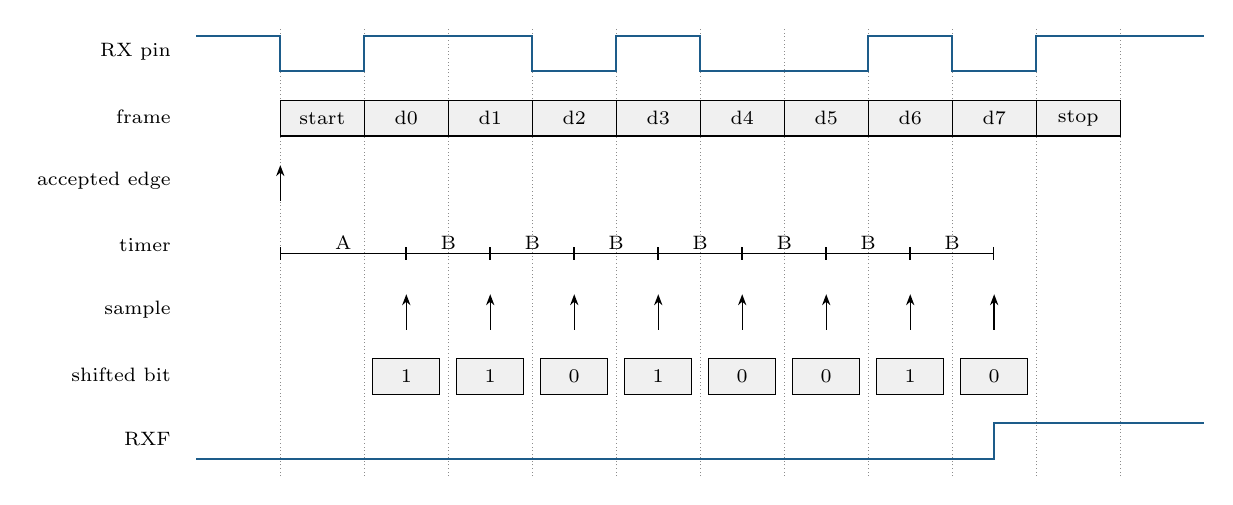
\begin{tikzpicture}[x=1mm,y=1mm]
\draw[densely dotted,line width=0.3pt,black!45] (37.67,1.00) -- (37.67,57.90);
\draw[densely dotted,line width=0.3pt,black!45] (48.33,1.00) -- (48.33,57.90);
\draw[densely dotted,line width=0.3pt,black!45] (59.00,1.00) -- (59.00,57.90);
\draw[densely dotted,line width=0.3pt,black!45] (69.67,1.00) -- (69.67,57.90);
\draw[densely dotted,line width=0.3pt,black!45] (80.33,1.00) -- (80.33,57.90);
\draw[densely dotted,line width=0.3pt,black!45] (91.00,1.00) -- (91.00,57.90);
\draw[densely dotted,line width=0.3pt,black!45] (101.67,1.00) -- (101.67,57.90);
\draw[densely dotted,line width=0.3pt,black!45] (112.33,1.00) -- (112.33,57.90);
\draw[densely dotted,line width=0.3pt,black!45] (123.00,1.00) -- (123.00,57.90);
\draw[densely dotted,line width=0.3pt,black!45] (133.67,1.00) -- (133.67,57.90);
\draw[densely dotted,line width=0.3pt,black!45] (144.33,1.00) -- (144.33,57.90);
\node[lbl,anchor=east] at (25.00,54.90) {RX pin};
\draw[line width=0.7pt,accent] (27.00,56.90) -- (37.67,56.90) -- (37.67,52.40) -- (48.33,52.40) -- (48.33,56.90) -- (59.00,56.90) -- (59.00,56.90) -- (69.67,56.90) -- (69.67,52.40) -- (80.33,52.40) -- (80.33,56.90) -- (91.00,56.90) -- (91.00,52.40) -- (101.67,52.40) -- (101.67,52.40) -- (112.33,52.40) -- (112.33,56.90) -- (123.00,56.90) -- (123.00,52.40) -- (133.67,52.40) -- (133.67,56.90) -- (155.00,56.90);
\node[lbl,anchor=east] at (25.00,46.70) {frame};
\draw[line width=0.4pt,fill=fillD] (37.67,44.20) rectangle (48.33,48.70);
\node[lbl,inner sep=0pt] at (43.00,46.45) {start};
\draw[line width=0.4pt,fill=fillD] (48.33,44.20) rectangle (59.00,48.70);
\node[lbl,inner sep=0pt] at (53.67,46.45) {d0};
\draw[line width=0.4pt,fill=fillD] (59.00,44.20) rectangle (69.67,48.70);
\node[lbl,inner sep=0pt] at (64.33,46.45) {d1};
\draw[line width=0.4pt,fill=fillD] (69.67,44.20) rectangle (80.33,48.70);
\node[lbl,inner sep=0pt] at (75.00,46.45) {d2};
\draw[line width=0.4pt,fill=fillD] (80.33,44.20) rectangle (91.00,48.70);
\node[lbl,inner sep=0pt] at (85.67,46.45) {d3};
\draw[line width=0.4pt,fill=fillD] (91.00,44.20) rectangle (101.67,48.70);
\node[lbl,inner sep=0pt] at (96.33,46.45) {d4};
\draw[line width=0.4pt,fill=fillD] (101.67,44.20) rectangle (112.33,48.70);
\node[lbl,inner sep=0pt] at (107.00,46.45) {d5};
\draw[line width=0.4pt,fill=fillD] (112.33,44.20) rectangle (123.00,48.70);
\node[lbl,inner sep=0pt] at (117.67,46.45) {d6};
\draw[line width=0.4pt,fill=fillD] (123.00,44.20) rectangle (133.67,48.70);
\node[lbl,inner sep=0pt] at (128.33,46.45) {d7};
\draw[line width=0.4pt,fill=fillD] (133.67,44.20) rectangle (144.33,48.70);
\node[lbl,inner sep=0pt] at (139.00,46.45) {stop};
\node[lbl,anchor=east] at (25.00,38.50) {accepted edge};
\draw[-{Stealth[length=1.4mm]},line width=0.5pt] (37.67,36.00) -- (37.67,40.50);
\node[lbl,anchor=east] at (25.00,30.30) {timer};
\draw[|-|,line width=0.4pt] (37.67,29.30) -- (53.67,29.30);
\node[lbl,anchor=south,inner sep=0.6pt] at (45.67,29.50) {A};
\draw[|-|,line width=0.4pt] (53.67,29.30) -- (64.33,29.30);
\node[lbl,anchor=south,inner sep=0.6pt] at (59.00,29.50) {B};
\draw[|-|,line width=0.4pt] (64.33,29.30) -- (75.00,29.30);
\node[lbl,anchor=south,inner sep=0.6pt] at (69.67,29.50) {B};
\draw[|-|,line width=0.4pt] (75.00,29.30) -- (85.67,29.30);
\node[lbl,anchor=south,inner sep=0.6pt] at (80.33,29.50) {B};
\draw[|-|,line width=0.4pt] (85.67,29.30) -- (96.33,29.30);
\node[lbl,anchor=south,inner sep=0.6pt] at (91.00,29.50) {B};
\draw[|-|,line width=0.4pt] (96.33,29.30) -- (107.00,29.30);
\node[lbl,anchor=south,inner sep=0.6pt] at (101.67,29.50) {B};
\draw[|-|,line width=0.4pt] (107.00,29.30) -- (117.67,29.30);
\node[lbl,anchor=south,inner sep=0.6pt] at (112.33,29.50) {B};
\draw[|-|,line width=0.4pt] (117.67,29.30) -- (128.33,29.30);
\node[lbl,anchor=south,inner sep=0.6pt] at (123.00,29.50) {B};
\node[lbl,anchor=east] at (25.00,22.10) {sample};
\draw[-{Stealth[length=1.4mm]},line width=0.5pt] (53.67,19.60) -- (53.67,24.10);
\draw[-{Stealth[length=1.4mm]},line width=0.5pt] (64.33,19.60) -- (64.33,24.10);
\draw[-{Stealth[length=1.4mm]},line width=0.5pt] (75.00,19.60) -- (75.00,24.10);
\draw[-{Stealth[length=1.4mm]},line width=0.5pt] (85.67,19.60) -- (85.67,24.10);
\draw[-{Stealth[length=1.4mm]},line width=0.5pt] (96.33,19.60) -- (96.33,24.10);
\draw[-{Stealth[length=1.4mm]},line width=0.5pt] (107.00,19.60) -- (107.00,24.10);
\draw[-{Stealth[length=1.4mm]},line width=0.5pt] (117.67,19.60) -- (117.67,24.10);
\draw[-{Stealth[length=1.4mm]},line width=0.5pt] (128.33,19.60) -- (128.33,24.10);
\node[lbl,anchor=east] at (25.00,13.90) {shifted bit};
\draw[line width=0.4pt,fill=fillD] (49.40,11.40) rectangle (57.93,15.90);
\node[lbl,inner sep=0pt] at (53.67,13.65) {1};
\draw[line width=0.4pt,fill=fillD] (60.07,11.40) rectangle (68.60,15.90);
\node[lbl,inner sep=0pt] at (64.33,13.65) {1};
\draw[line width=0.4pt,fill=fillD] (70.73,11.40) rectangle (79.27,15.90);
\node[lbl,inner sep=0pt] at (75.00,13.65) {0};
\draw[line width=0.4pt,fill=fillD] (81.40,11.40) rectangle (89.93,15.90);
\node[lbl,inner sep=0pt] at (85.67,13.65) {1};
\draw[line width=0.4pt,fill=fillD] (92.07,11.40) rectangle (100.60,15.90);
\node[lbl,inner sep=0pt] at (96.33,13.65) {0};
\draw[line width=0.4pt,fill=fillD] (102.73,11.40) rectangle (111.27,15.90);
\node[lbl,inner sep=0pt] at (107.00,13.65) {0};
\draw[line width=0.4pt,fill=fillD] (113.40,11.40) rectangle (121.93,15.90);
\node[lbl,inner sep=0pt] at (117.67,13.65) {1};
\draw[line width=0.4pt,fill=fillD] (124.07,11.40) rectangle (132.60,15.90);
\node[lbl,inner sep=0pt] at (128.33,13.65) {0};
\node[lbl,anchor=east] at (25.00,5.70) {RXF};
\draw[line width=0.7pt,accent] (27.00,3.20) -- (128.33,3.20) -- (128.33,7.70) -- (155.00,7.70);
\end{tikzpicture}
\caption{UART receive of the byte \texttt{0x4B}. Dotted lines are bit boundaries.}
\label{fig:uartrx}
\end{figure}

\textbf{Transmit.} \reg{TXEN}; B = 1 bit; \reg{LCENC} = NRZ; \reg{SS} set, so the cell adds a start bit and a
stop bit; \reg{IDLE} = high. Writing \reg{LTnDATA} starts the frame. The stop bit is not checked and the start bit is not validated; see section~\ref{sec:lcext}.


\begin{figure}[H]
\centering
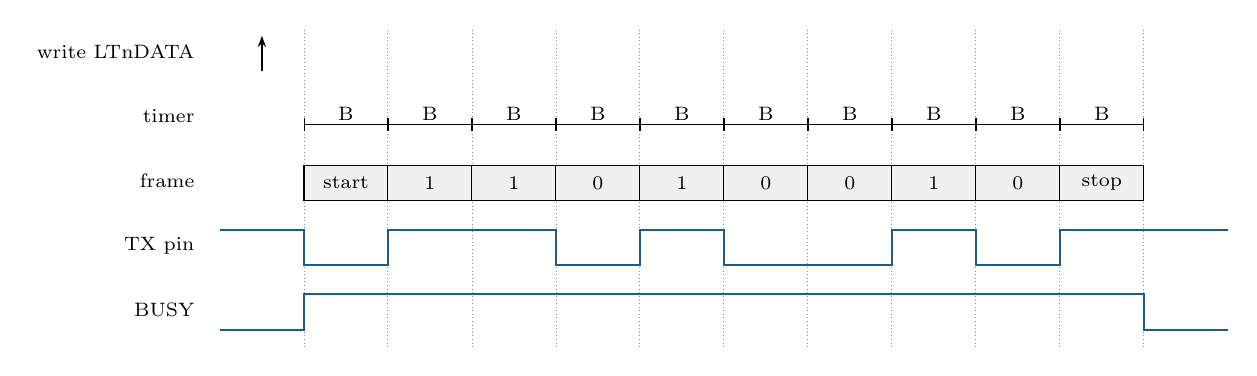
\begin{tikzpicture}[x=1mm,y=1mm]
\draw[densely dotted,line width=0.3pt,black!45] (37.67,1.00) -- (37.67,41.50);
\draw[densely dotted,line width=0.3pt,black!45] (48.33,1.00) -- (48.33,41.50);
\draw[densely dotted,line width=0.3pt,black!45] (59.00,1.00) -- (59.00,41.50);
\draw[densely dotted,line width=0.3pt,black!45] (69.67,1.00) -- (69.67,41.50);
\draw[densely dotted,line width=0.3pt,black!45] (80.33,1.00) -- (80.33,41.50);
\draw[densely dotted,line width=0.3pt,black!45] (91.00,1.00) -- (91.00,41.50);
\draw[densely dotted,line width=0.3pt,black!45] (101.67,1.00) -- (101.67,41.50);
\draw[densely dotted,line width=0.3pt,black!45] (112.33,1.00) -- (112.33,41.50);
\draw[densely dotted,line width=0.3pt,black!45] (123.00,1.00) -- (123.00,41.50);
\draw[densely dotted,line width=0.3pt,black!45] (133.67,1.00) -- (133.67,41.50);
\draw[densely dotted,line width=0.3pt,black!45] (144.33,1.00) -- (144.33,41.50);
\node[lbl,anchor=east] at (25.00,38.50) {write LTnDATA};
\draw[-{Stealth[length=1.4mm]},line width=0.5pt] (32.33,36.00) -- (32.33,40.50);
\node[lbl,anchor=east] at (25.00,30.30) {timer};
\draw[|-|,line width=0.4pt] (37.67,29.30) -- (48.33,29.30);
\node[lbl,anchor=south,inner sep=0.6pt] at (43.00,29.50) {B};
\draw[|-|,line width=0.4pt] (48.33,29.30) -- (59.00,29.30);
\node[lbl,anchor=south,inner sep=0.6pt] at (53.67,29.50) {B};
\draw[|-|,line width=0.4pt] (59.00,29.30) -- (69.67,29.30);
\node[lbl,anchor=south,inner sep=0.6pt] at (64.33,29.50) {B};
\draw[|-|,line width=0.4pt] (69.67,29.30) -- (80.33,29.30);
\node[lbl,anchor=south,inner sep=0.6pt] at (75.00,29.50) {B};
\draw[|-|,line width=0.4pt] (80.33,29.30) -- (91.00,29.30);
\node[lbl,anchor=south,inner sep=0.6pt] at (85.67,29.50) {B};
\draw[|-|,line width=0.4pt] (91.00,29.30) -- (101.67,29.30);
\node[lbl,anchor=south,inner sep=0.6pt] at (96.33,29.50) {B};
\draw[|-|,line width=0.4pt] (101.67,29.30) -- (112.33,29.30);
\node[lbl,anchor=south,inner sep=0.6pt] at (107.00,29.50) {B};
\draw[|-|,line width=0.4pt] (112.33,29.30) -- (123.00,29.30);
\node[lbl,anchor=south,inner sep=0.6pt] at (117.67,29.50) {B};
\draw[|-|,line width=0.4pt] (123.00,29.30) -- (133.67,29.30);
\node[lbl,anchor=south,inner sep=0.6pt] at (128.33,29.50) {B};
\draw[|-|,line width=0.4pt] (133.67,29.30) -- (144.33,29.30);
\node[lbl,anchor=south,inner sep=0.6pt] at (139.00,29.50) {B};
\node[lbl,anchor=east] at (25.00,22.10) {frame};
\draw[line width=0.4pt,fill=fillD] (37.67,19.60) rectangle (48.33,24.10);
\node[lbl,inner sep=0pt] at (43.00,21.85) {start};
\draw[line width=0.4pt,fill=fillD] (48.33,19.60) rectangle (59.00,24.10);
\node[lbl,inner sep=0pt] at (53.67,21.85) {1};
\draw[line width=0.4pt,fill=fillD] (59.00,19.60) rectangle (69.67,24.10);
\node[lbl,inner sep=0pt] at (64.33,21.85) {1};
\draw[line width=0.4pt,fill=fillD] (69.67,19.60) rectangle (80.33,24.10);
\node[lbl,inner sep=0pt] at (75.00,21.85) {0};
\draw[line width=0.4pt,fill=fillD] (80.33,19.60) rectangle (91.00,24.10);
\node[lbl,inner sep=0pt] at (85.67,21.85) {1};
\draw[line width=0.4pt,fill=fillD] (91.00,19.60) rectangle (101.67,24.10);
\node[lbl,inner sep=0pt] at (96.33,21.85) {0};
\draw[line width=0.4pt,fill=fillD] (101.67,19.60) rectangle (112.33,24.10);
\node[lbl,inner sep=0pt] at (107.00,21.85) {0};
\draw[line width=0.4pt,fill=fillD] (112.33,19.60) rectangle (123.00,24.10);
\node[lbl,inner sep=0pt] at (117.67,21.85) {1};
\draw[line width=0.4pt,fill=fillD] (123.00,19.60) rectangle (133.67,24.10);
\node[lbl,inner sep=0pt] at (128.33,21.85) {0};
\draw[line width=0.4pt,fill=fillD] (133.67,19.60) rectangle (144.33,24.10);
\node[lbl,inner sep=0pt] at (139.00,21.85) {stop};
\node[lbl,anchor=east] at (25.00,13.90) {TX pin};
\draw[line width=0.7pt,accent] (27.00,15.90) -- (37.67,15.90) -- (37.67,11.40) -- (48.33,11.40) -- (48.33,15.90) -- (59.00,15.90) -- (59.00,15.90) -- (69.67,15.90) -- (69.67,11.40) -- (80.33,11.40) -- (80.33,15.90) -- (91.00,15.90) -- (91.00,11.40) -- (101.67,11.40) -- (101.67,11.40) -- (112.33,11.40) -- (112.33,15.90) -- (123.00,15.90) -- (123.00,11.40) -- (133.67,11.40) -- (133.67,15.90) -- (155.00,15.90);
\node[lbl,anchor=east] at (25.00,5.70) {BUSY};
\draw[line width=0.7pt,accent] (27.00,3.20) -- (37.67,3.20) -- (37.67,7.70) -- (144.33,7.70) -- (144.33,3.20) -- (155.00,3.20);
\end{tikzpicture}
\caption{UART transmit of the same byte.}
\label{fig:uarttx}
\end{figure}

\subsection{SPI}

\textbf{Master, mode 0, with the two cells of a pair.} Transmit cell: \reg{TWOPH} with B = half a clock
period; second output function = bit clock, idle low; \reg{LCENC} = level; most significant bit first. Receive
cell: \reg{TRIG} = 2, so it samples in the middle of each transmitted bit; \reg{LCDEC} = level. As slave, both
cells take the clock pin as trigger and need no timer.


\begin{figure}[H]
\centering
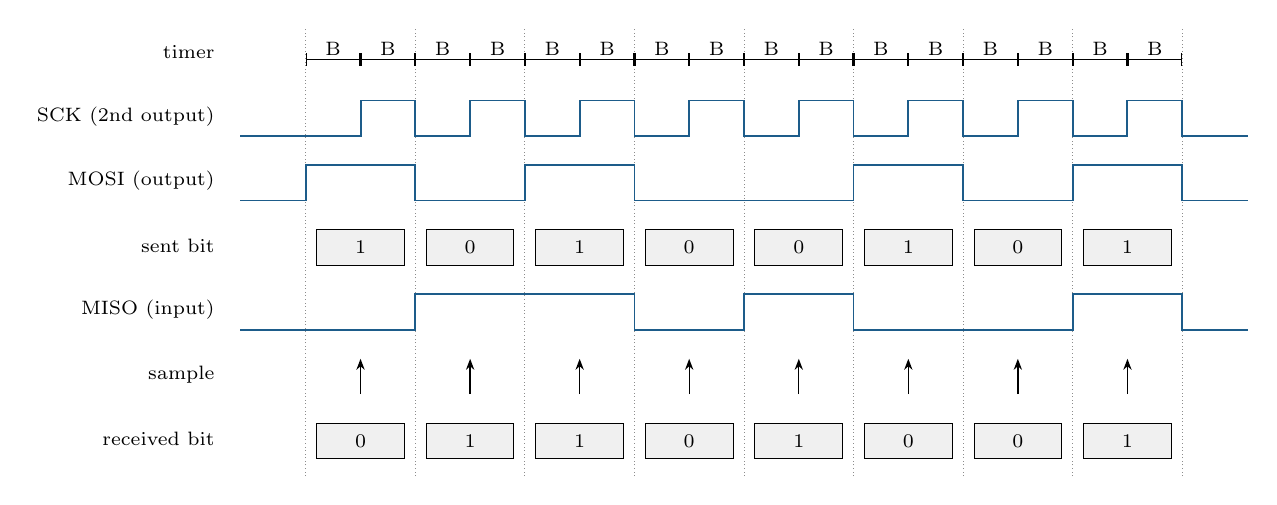
\begin{tikzpicture}[x=1mm,y=1mm]
\draw[densely dotted,line width=0.3pt,black!45] (35.35,1.00) -- (35.35,57.90);
\draw[densely dotted,line width=0.3pt,black!45] (49.26,1.00) -- (49.26,57.90);
\draw[densely dotted,line width=0.3pt,black!45] (63.17,1.00) -- (63.17,57.90);
\draw[densely dotted,line width=0.3pt,black!45] (77.09,1.00) -- (77.09,57.90);
\draw[densely dotted,line width=0.3pt,black!45] (91.00,1.00) -- (91.00,57.90);
\draw[densely dotted,line width=0.3pt,black!45] (104.91,1.00) -- (104.91,57.90);
\draw[densely dotted,line width=0.3pt,black!45] (118.83,1.00) -- (118.83,57.90);
\draw[densely dotted,line width=0.3pt,black!45] (132.74,1.00) -- (132.74,57.90);
\draw[densely dotted,line width=0.3pt,black!45] (146.65,1.00) -- (146.65,57.90);
\node[lbl,anchor=east] at (25.00,54.90) {timer};
\draw[|-|,line width=0.4pt] (35.35,53.90) -- (42.30,53.90);
\node[lbl,anchor=south,inner sep=0.6pt] at (38.83,54.10) {B};
\draw[|-|,line width=0.4pt] (42.30,53.90) -- (49.26,53.90);
\node[lbl,anchor=south,inner sep=0.6pt] at (45.78,54.10) {B};
\draw[|-|,line width=0.4pt] (49.26,53.90) -- (56.22,53.90);
\node[lbl,anchor=south,inner sep=0.6pt] at (52.74,54.10) {B};
\draw[|-|,line width=0.4pt] (56.22,53.90) -- (63.17,53.90);
\node[lbl,anchor=south,inner sep=0.6pt] at (59.70,54.10) {B};
\draw[|-|,line width=0.4pt] (63.17,53.90) -- (70.13,53.90);
\node[lbl,anchor=south,inner sep=0.6pt] at (66.65,54.10) {B};
\draw[|-|,line width=0.4pt] (70.13,53.90) -- (77.09,53.90);
\node[lbl,anchor=south,inner sep=0.6pt] at (73.61,54.10) {B};
\draw[|-|,line width=0.4pt] (77.09,53.90) -- (84.04,53.90);
\node[lbl,anchor=south,inner sep=0.6pt] at (80.57,54.10) {B};
\draw[|-|,line width=0.4pt] (84.04,53.90) -- (91.00,53.90);
\node[lbl,anchor=south,inner sep=0.6pt] at (87.52,54.10) {B};
\draw[|-|,line width=0.4pt] (91.00,53.90) -- (97.96,53.90);
\node[lbl,anchor=south,inner sep=0.6pt] at (94.48,54.10) {B};
\draw[|-|,line width=0.4pt] (97.96,53.90) -- (104.91,53.90);
\node[lbl,anchor=south,inner sep=0.6pt] at (101.43,54.10) {B};
\draw[|-|,line width=0.4pt] (104.91,53.90) -- (111.87,53.90);
\node[lbl,anchor=south,inner sep=0.6pt] at (108.39,54.10) {B};
\draw[|-|,line width=0.4pt] (111.87,53.90) -- (118.83,53.90);
\node[lbl,anchor=south,inner sep=0.6pt] at (115.35,54.10) {B};
\draw[|-|,line width=0.4pt] (118.83,53.90) -- (125.78,53.90);
\node[lbl,anchor=south,inner sep=0.6pt] at (122.30,54.10) {B};
\draw[|-|,line width=0.4pt] (125.78,53.90) -- (132.74,53.90);
\node[lbl,anchor=south,inner sep=0.6pt] at (129.26,54.10) {B};
\draw[|-|,line width=0.4pt] (132.74,53.90) -- (139.70,53.90);
\node[lbl,anchor=south,inner sep=0.6pt] at (136.22,54.10) {B};
\draw[|-|,line width=0.4pt] (139.70,53.90) -- (146.65,53.90);
\node[lbl,anchor=south,inner sep=0.6pt] at (143.17,54.10) {B};
\node[lbl,anchor=east] at (25.00,46.70) {SCK (2nd output)};
\draw[line width=0.7pt,accent] (27.00,44.20) -- (42.30,44.20) -- (42.30,48.70) -- (49.26,48.70) -- (49.26,44.20) -- (56.22,44.20) -- (56.22,48.70) -- (63.17,48.70) -- (63.17,44.20) -- (70.13,44.20) -- (70.13,48.70) -- (77.09,48.70) -- (77.09,44.20) -- (84.04,44.20) -- (84.04,48.70) -- (91.00,48.70) -- (91.00,44.20) -- (97.96,44.20) -- (97.96,48.70) -- (104.91,48.70) -- (104.91,44.20) -- (111.87,44.20) -- (111.87,48.70) -- (118.83,48.70) -- (118.83,44.20) -- (125.78,44.20) -- (125.78,48.70) -- (132.74,48.70) -- (132.74,44.20) -- (139.70,44.20) -- (139.70,48.70) -- (146.65,48.70) -- (146.65,44.20) -- (155.00,44.20);
\node[lbl,anchor=east] at (25.00,38.50) {MOSI (output)};
\draw[line width=0.7pt,accent] (27.00,36.00) -- (35.35,36.00) -- (35.35,40.50) -- (49.26,40.50) -- (49.26,36.00) -- (63.17,36.00) -- (63.17,40.50) -- (77.09,40.50) -- (77.09,36.00) -- (91.00,36.00) -- (91.00,36.00) -- (104.91,36.00) -- (104.91,40.50) -- (118.83,40.50) -- (118.83,36.00) -- (132.74,36.00) -- (132.74,40.50) -- (146.65,40.50) -- (146.65,36.00) -- (155.00,36.00);
\node[lbl,anchor=east] at (25.00,30.30) {sent bit};
\draw[line width=0.4pt,fill=fillD] (36.74,27.80) rectangle (47.87,32.30);
\node[lbl,inner sep=0pt] at (42.30,30.05) {1};
\draw[line width=0.4pt,fill=fillD] (50.65,27.80) rectangle (61.78,32.30);
\node[lbl,inner sep=0pt] at (56.22,30.05) {0};
\draw[line width=0.4pt,fill=fillD] (64.57,27.80) rectangle (75.70,32.30);
\node[lbl,inner sep=0pt] at (70.13,30.05) {1};
\draw[line width=0.4pt,fill=fillD] (78.48,27.80) rectangle (89.61,32.30);
\node[lbl,inner sep=0pt] at (84.04,30.05) {0};
\draw[line width=0.4pt,fill=fillD] (92.39,27.80) rectangle (103.52,32.30);
\node[lbl,inner sep=0pt] at (97.96,30.05) {0};
\draw[line width=0.4pt,fill=fillD] (106.30,27.80) rectangle (117.43,32.30);
\node[lbl,inner sep=0pt] at (111.87,30.05) {1};
\draw[line width=0.4pt,fill=fillD] (120.22,27.80) rectangle (131.35,32.30);
\node[lbl,inner sep=0pt] at (125.78,30.05) {0};
\draw[line width=0.4pt,fill=fillD] (134.13,27.80) rectangle (145.26,32.30);
\node[lbl,inner sep=0pt] at (139.70,30.05) {1};
\node[lbl,anchor=east] at (25.00,22.10) {MISO (input)};
\draw[line width=0.7pt,accent] (27.00,19.60) -- (35.35,19.60) -- (35.35,19.60) -- (49.26,19.60) -- (49.26,24.10) -- (63.17,24.10) -- (63.17,24.10) -- (77.09,24.10) -- (77.09,19.60) -- (91.00,19.60) -- (91.00,24.10) -- (104.91,24.10) -- (104.91,19.60) -- (118.83,19.60) -- (118.83,19.60) -- (132.74,19.60) -- (132.74,24.10) -- (146.65,24.10) -- (146.65,19.60) -- (155.00,19.60);
\node[lbl,anchor=east] at (25.00,13.90) {sample};
\draw[-{Stealth[length=1.4mm]},line width=0.5pt] (42.30,11.40) -- (42.30,15.90);
\draw[-{Stealth[length=1.4mm]},line width=0.5pt] (56.22,11.40) -- (56.22,15.90);
\draw[-{Stealth[length=1.4mm]},line width=0.5pt] (70.13,11.40) -- (70.13,15.90);
\draw[-{Stealth[length=1.4mm]},line width=0.5pt] (84.04,11.40) -- (84.04,15.90);
\draw[-{Stealth[length=1.4mm]},line width=0.5pt] (97.96,11.40) -- (97.96,15.90);
\draw[-{Stealth[length=1.4mm]},line width=0.5pt] (111.87,11.40) -- (111.87,15.90);
\draw[-{Stealth[length=1.4mm]},line width=0.5pt] (125.78,11.40) -- (125.78,15.90);
\draw[-{Stealth[length=1.4mm]},line width=0.5pt] (139.70,11.40) -- (139.70,15.90);
\node[lbl,anchor=east] at (25.00,5.70) {received bit};
\draw[line width=0.4pt,fill=fillD] (36.74,3.20) rectangle (47.87,7.70);
\node[lbl,inner sep=0pt] at (42.30,5.45) {0};
\draw[line width=0.4pt,fill=fillD] (50.65,3.20) rectangle (61.78,7.70);
\node[lbl,inner sep=0pt] at (56.22,5.45) {1};
\draw[line width=0.4pt,fill=fillD] (64.57,3.20) rectangle (75.70,7.70);
\node[lbl,inner sep=0pt] at (70.13,5.45) {1};
\draw[line width=0.4pt,fill=fillD] (78.48,3.20) rectangle (89.61,7.70);
\node[lbl,inner sep=0pt] at (84.04,5.45) {0};
\draw[line width=0.4pt,fill=fillD] (92.39,3.20) rectangle (103.52,7.70);
\node[lbl,inner sep=0pt] at (97.96,5.45) {1};
\draw[line width=0.4pt,fill=fillD] (106.30,3.20) rectangle (117.43,7.70);
\node[lbl,inner sep=0pt] at (111.87,5.45) {0};
\draw[line width=0.4pt,fill=fillD] (120.22,3.20) rectangle (131.35,7.70);
\node[lbl,inner sep=0pt] at (125.78,5.45) {0};
\draw[line width=0.4pt,fill=fillD] (134.13,3.20) rectangle (145.26,7.70);
\node[lbl,inner sep=0pt] at (139.70,5.45) {1};
\end{tikzpicture}
\caption{SPI exchange of one byte: \texttt{0xA5} out, \texttt{0x69} in.}
\label{fig:spi}
\end{figure}

\subsection{I2C}

I2C runs in firmware at 100 and 400\,kHz. The cell can take over the eight data bits of a byte.

\textbf{Slave receive.} \reg{RXEN}; clock pin = SCL with \reg{EDGE} = rising and the shift trigger on the pin
edge; \reg{LEN} = 8, most significant bit first. Firmware detects the start condition with the pin-change
event, and drives the acknowledge bit through the port register. For transmit, the same setting with
\reg{TXEN} shifts a byte out on the falling edges of SCL, with the pin configured as open drain.


\begin{figure}[H]
\centering
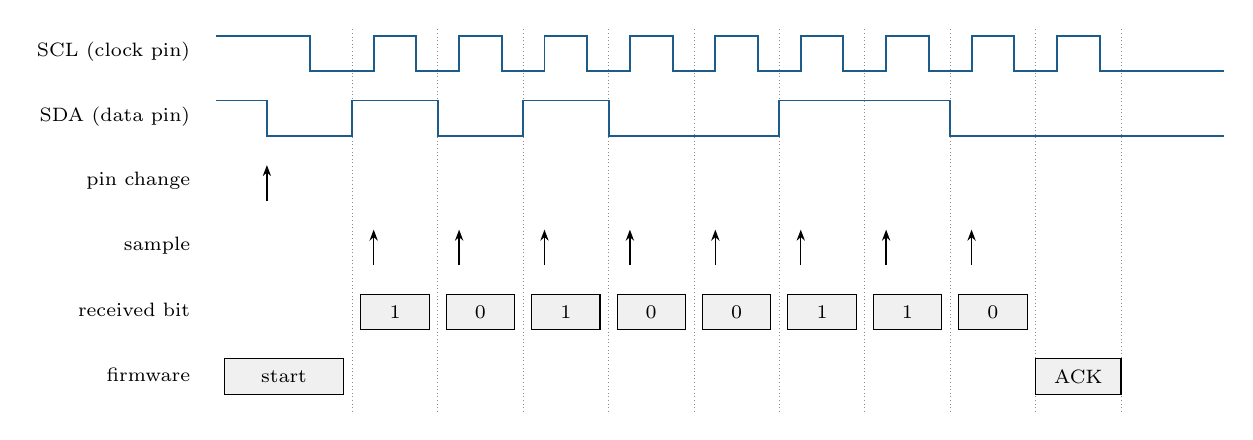
\begin{tikzpicture}[x=1mm,y=1mm]
\draw[densely dotted,line width=0.3pt,black!45] (44.36,1.00) -- (44.36,49.70);
\draw[densely dotted,line width=0.3pt,black!45] (55.20,1.00) -- (55.20,49.70);
\draw[densely dotted,line width=0.3pt,black!45] (66.05,1.00) -- (66.05,49.70);
\draw[densely dotted,line width=0.3pt,black!45] (76.90,1.00) -- (76.90,49.70);
\draw[densely dotted,line width=0.3pt,black!45] (87.75,1.00) -- (87.75,49.70);
\draw[densely dotted,line width=0.3pt,black!45] (98.59,1.00) -- (98.59,49.70);
\draw[densely dotted,line width=0.3pt,black!45] (109.44,1.00) -- (109.44,49.70);
\draw[densely dotted,line width=0.3pt,black!45] (120.29,1.00) -- (120.29,49.70);
\draw[densely dotted,line width=0.3pt,black!45] (131.14,1.00) -- (131.14,49.70);
\draw[densely dotted,line width=0.3pt,black!45] (141.98,1.00) -- (141.98,49.70);
\node[lbl,anchor=east] at (25.00,46.70) {SCL (clock pin)};
\draw[line width=0.7pt,accent] (27.00,48.70) -- (38.93,48.70) -- (38.93,44.20) -- (47.07,44.20) -- (47.07,48.70) -- (52.49,48.70) -- (52.49,44.20) -- (57.92,44.20) -- (57.92,48.70) -- (63.34,48.70) -- (63.34,44.20) -- (68.76,44.20) -- (68.76,48.70) -- (74.19,48.70) -- (74.19,44.20) -- (79.61,44.20) -- (79.61,48.70) -- (85.03,48.70) -- (85.03,44.20) -- (90.46,44.20) -- (90.46,48.70) -- (95.88,48.70) -- (95.88,44.20) -- (101.31,44.20) -- (101.31,48.70) -- (106.73,48.70) -- (106.73,44.20) -- (112.15,44.20) -- (112.15,48.70) -- (117.58,48.70) -- (117.58,44.20) -- (123.00,44.20) -- (123.00,48.70) -- (128.42,48.70) -- (128.42,44.20) -- (133.85,44.20) -- (133.85,48.70) -- (139.27,48.70) -- (139.27,44.20) -- (155.00,44.20);
\node[lbl,anchor=east] at (25.00,38.50) {SDA (data pin)};
\draw[line width=0.7pt,accent] (27.00,40.50) -- (33.51,40.50) -- (33.51,36.00) -- (44.36,36.00) -- (44.36,40.50) -- (55.20,40.50) -- (55.20,36.00) -- (66.05,36.00) -- (66.05,40.50) -- (76.90,40.50) -- (76.90,36.00) -- (87.75,36.00) -- (87.75,36.00) -- (98.59,36.00) -- (98.59,40.50) -- (109.44,40.50) -- (109.44,40.50) -- (120.29,40.50) -- (120.29,36.00) -- (131.14,36.00) -- (131.14,36.00) -- (155.00,36.00);
\node[lbl,anchor=east] at (25.00,30.30) {pin change};
\draw[-{Stealth[length=1.4mm]},line width=0.5pt] (33.51,27.80) -- (33.51,32.30);
\node[lbl,anchor=east] at (25.00,22.10) {sample};
\draw[-{Stealth[length=1.4mm]},line width=0.5pt] (47.07,19.60) -- (47.07,24.10);
\draw[-{Stealth[length=1.4mm]},line width=0.5pt] (57.92,19.60) -- (57.92,24.10);
\draw[-{Stealth[length=1.4mm]},line width=0.5pt] (68.76,19.60) -- (68.76,24.10);
\draw[-{Stealth[length=1.4mm]},line width=0.5pt] (79.61,19.60) -- (79.61,24.10);
\draw[-{Stealth[length=1.4mm]},line width=0.5pt] (90.46,19.60) -- (90.46,24.10);
\draw[-{Stealth[length=1.4mm]},line width=0.5pt] (101.31,19.60) -- (101.31,24.10);
\draw[-{Stealth[length=1.4mm]},line width=0.5pt] (112.15,19.60) -- (112.15,24.10);
\draw[-{Stealth[length=1.4mm]},line width=0.5pt] (123.00,19.60) -- (123.00,24.10);
\node[lbl,anchor=east] at (25.00,13.90) {received bit};
\draw[line width=0.4pt,fill=fillD] (45.44,11.40) rectangle (54.12,15.90);
\node[lbl,inner sep=0pt] at (49.78,13.65) {1};
\draw[line width=0.4pt,fill=fillD] (56.29,11.40) rectangle (64.97,15.90);
\node[lbl,inner sep=0pt] at (60.63,13.65) {0};
\draw[line width=0.4pt,fill=fillD] (67.14,11.40) rectangle (75.81,15.90);
\node[lbl,inner sep=0pt] at (71.47,13.65) {1};
\draw[line width=0.4pt,fill=fillD] (77.98,11.40) rectangle (86.66,15.90);
\node[lbl,inner sep=0pt] at (82.32,13.65) {0};
\draw[line width=0.4pt,fill=fillD] (88.83,11.40) rectangle (97.51,15.90);
\node[lbl,inner sep=0pt] at (93.17,13.65) {0};
\draw[line width=0.4pt,fill=fillD] (99.68,11.40) rectangle (108.36,15.90);
\node[lbl,inner sep=0pt] at (104.02,13.65) {1};
\draw[line width=0.4pt,fill=fillD] (110.53,11.40) rectangle (119.20,15.90);
\node[lbl,inner sep=0pt] at (114.86,13.65) {1};
\draw[line width=0.4pt,fill=fillD] (121.37,11.40) rectangle (130.05,15.90);
\node[lbl,inner sep=0pt] at (125.71,13.65) {0};
\node[lbl,anchor=east] at (25.00,5.70) {firmware};
\draw[line width=0.4pt,fill=fillD] (28.08,3.20) rectangle (43.27,7.70);
\node[lbl,inner sep=0pt] at (35.68,5.45) {start};
\draw[line width=0.4pt,fill=fillD] (131.14,3.20) rectangle (141.98,7.70);
\node[lbl,inner sep=0pt] at (136.56,5.45) {ACK};
\end{tikzpicture}
\caption{I2C slave receiving the byte \texttt{0xA6}. The acknowledge bit is driven by firmware.}
\label{fig:i2c}
\end{figure}

\subsection{WS2812}

\textbf{Receive (as LED).} \reg{EDGE} = rising, accepted only while waiting; \reg{STOP} = after each sample;
A = 36 clock cycles (0.6\,$\mu$s); \reg{LCDEC} = level; most significant bit first. Each rising edge starts the
timer. The level at expiry is the bit: a long pulse is still high, a short pulse has ended.


\begin{figure}[H]
\centering
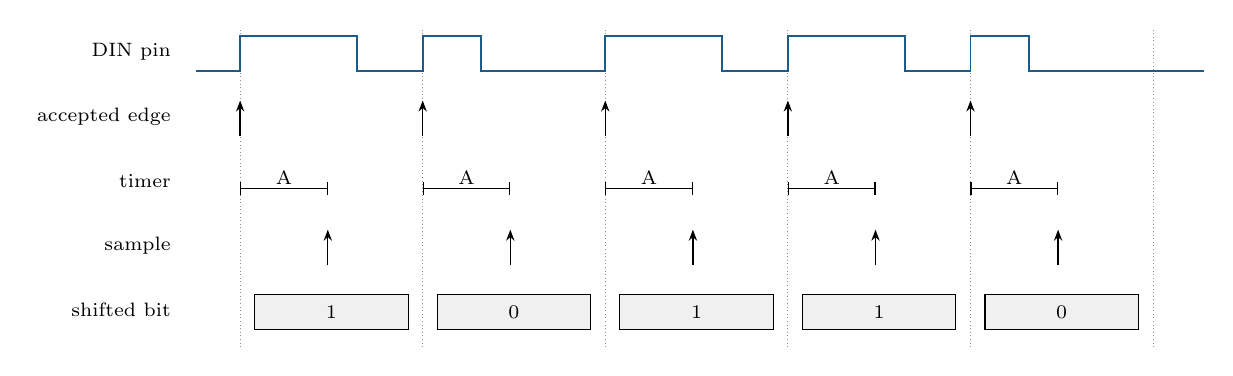
\begin{tikzpicture}[x=1mm,y=1mm]
\draw[densely dotted,line width=0.3pt,black!45] (32.57,1.00) -- (32.57,41.50);
\draw[densely dotted,line width=0.3pt,black!45] (55.75,1.00) -- (55.75,41.50);
\draw[densely dotted,line width=0.3pt,black!45] (78.94,1.00) -- (78.94,41.50);
\draw[densely dotted,line width=0.3pt,black!45] (102.13,1.00) -- (102.13,41.50);
\draw[densely dotted,line width=0.3pt,black!45] (125.32,1.00) -- (125.32,41.50);
\draw[densely dotted,line width=0.3pt,black!45] (148.51,1.00) -- (148.51,41.50);
\node[lbl,anchor=east] at (25.00,38.50) {DIN pin};
\draw[line width=0.7pt,accent] (27.00,36.00) -- (32.57,36.00) -- (32.57,40.50) -- (47.41,40.50) -- (47.41,36.00) -- (55.75,36.00) -- (55.75,40.50) -- (63.17,40.50) -- (63.17,36.00) -- (78.94,36.00) -- (78.94,40.50) -- (93.78,40.50) -- (93.78,36.00) -- (102.13,36.00) -- (102.13,40.50) -- (116.97,40.50) -- (116.97,36.00) -- (125.32,36.00) -- (125.32,40.50) -- (132.74,40.50) -- (132.74,36.00) -- (155.00,36.00);
\node[lbl,anchor=east] at (25.00,30.30) {accepted edge};
\draw[-{Stealth[length=1.4mm]},line width=0.5pt] (32.57,27.80) -- (32.57,32.30);
\draw[-{Stealth[length=1.4mm]},line width=0.5pt] (55.75,27.80) -- (55.75,32.30);
\draw[-{Stealth[length=1.4mm]},line width=0.5pt] (78.94,27.80) -- (78.94,32.30);
\draw[-{Stealth[length=1.4mm]},line width=0.5pt] (102.13,27.80) -- (102.13,32.30);
\draw[-{Stealth[length=1.4mm]},line width=0.5pt] (125.32,27.80) -- (125.32,32.30);
\node[lbl,anchor=east] at (25.00,22.10) {timer};
\draw[|-|,line width=0.4pt] (32.57,21.10) -- (43.70,21.10);
\node[lbl,anchor=south,inner sep=0.6pt] at (38.13,21.30) {A};
\draw[|-|,line width=0.4pt] (55.75,21.10) -- (66.88,21.10);
\node[lbl,anchor=south,inner sep=0.6pt] at (61.32,21.30) {A};
\draw[|-|,line width=0.4pt] (78.94,21.10) -- (90.07,21.10);
\node[lbl,anchor=south,inner sep=0.6pt] at (84.51,21.30) {A};
\draw[|-|,line width=0.4pt] (102.13,21.10) -- (113.26,21.10);
\node[lbl,anchor=south,inner sep=0.6pt] at (107.70,21.30) {A};
\draw[|-|,line width=0.4pt] (125.32,21.10) -- (136.45,21.10);
\node[lbl,anchor=south,inner sep=0.6pt] at (130.88,21.30) {A};
\node[lbl,anchor=east] at (25.00,13.90) {sample};
\draw[-{Stealth[length=1.4mm]},line width=0.5pt] (43.70,11.40) -- (43.70,15.90);
\draw[-{Stealth[length=1.4mm]},line width=0.5pt] (66.88,11.40) -- (66.88,15.90);
\draw[-{Stealth[length=1.4mm]},line width=0.5pt] (90.07,11.40) -- (90.07,15.90);
\draw[-{Stealth[length=1.4mm]},line width=0.5pt] (113.26,11.40) -- (113.26,15.90);
\draw[-{Stealth[length=1.4mm]},line width=0.5pt] (136.45,11.40) -- (136.45,15.90);
\node[lbl,anchor=east] at (25.00,5.70) {shifted bit};
\draw[line width=0.4pt,fill=fillD] (34.42,3.20) rectangle (53.90,7.70);
\node[lbl,inner sep=0pt] at (44.16,5.45) {1};
\draw[line width=0.4pt,fill=fillD] (57.61,3.20) rectangle (77.09,7.70);
\node[lbl,inner sep=0pt] at (67.35,5.45) {0};
\draw[line width=0.4pt,fill=fillD] (80.80,3.20) rectangle (100.28,7.70);
\node[lbl,inner sep=0pt] at (90.54,5.45) {1};
\draw[line width=0.4pt,fill=fillD] (103.99,3.20) rectangle (123.46,7.70);
\node[lbl,inner sep=0pt] at (113.72,5.45) {1};
\draw[line width=0.4pt,fill=fillD] (127.17,3.20) rectangle (146.65,7.70);
\node[lbl,inner sep=0pt] at (136.91,5.45) {0};
\end{tikzpicture}
\caption{WS2812 receive of five bits. The bit period is 1.25\,$\mu$s.}
\label{fig:wsrx}
\end{figure}

\textbf{Transmit (as controller).} \reg{TXEN}; \reg{CMP} set; B = 75 (bit period), A = 48 (high time for a
one), C = 24 (high time for a zero).


\begin{figure}[H]
\centering
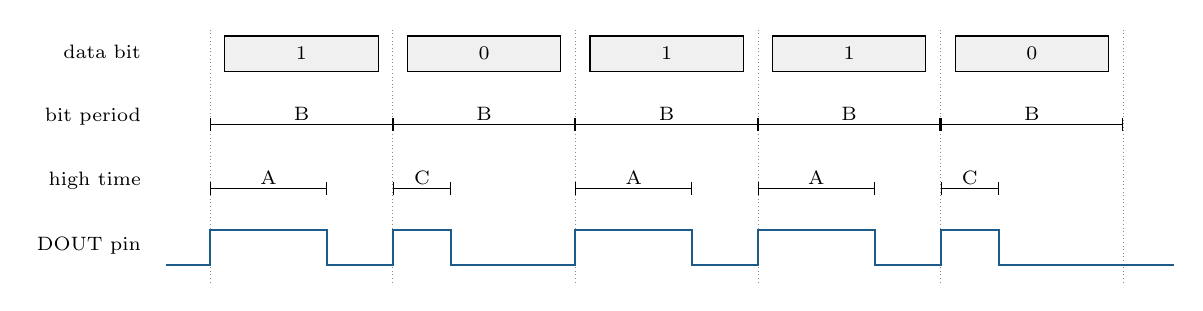
\begin{tikzpicture}[x=1mm,y=1mm]
\draw[densely dotted,line width=0.3pt,black!45] (32.57,1.00) -- (32.57,33.30);
\draw[densely dotted,line width=0.3pt,black!45] (55.75,1.00) -- (55.75,33.30);
\draw[densely dotted,line width=0.3pt,black!45] (78.94,1.00) -- (78.94,33.30);
\draw[densely dotted,line width=0.3pt,black!45] (102.13,1.00) -- (102.13,33.30);
\draw[densely dotted,line width=0.3pt,black!45] (125.32,1.00) -- (125.32,33.30);
\draw[densely dotted,line width=0.3pt,black!45] (148.51,1.00) -- (148.51,33.30);
\node[lbl,anchor=east] at (25.00,30.30) {data bit};
\draw[line width=0.4pt,fill=fillD] (34.42,27.80) rectangle (53.90,32.30);
\node[lbl,inner sep=0pt] at (44.16,30.05) {1};
\draw[line width=0.4pt,fill=fillD] (57.61,27.80) rectangle (77.09,32.30);
\node[lbl,inner sep=0pt] at (67.35,30.05) {0};
\draw[line width=0.4pt,fill=fillD] (80.80,27.80) rectangle (100.28,32.30);
\node[lbl,inner sep=0pt] at (90.54,30.05) {1};
\draw[line width=0.4pt,fill=fillD] (103.99,27.80) rectangle (123.46,32.30);
\node[lbl,inner sep=0pt] at (113.72,30.05) {1};
\draw[line width=0.4pt,fill=fillD] (127.17,27.80) rectangle (146.65,32.30);
\node[lbl,inner sep=0pt] at (136.91,30.05) {0};
\node[lbl,anchor=east] at (25.00,22.10) {bit period};
\draw[|-|,line width=0.4pt] (32.57,21.10) -- (55.75,21.10);
\node[lbl,anchor=south,inner sep=0.6pt] at (44.16,21.30) {B};
\draw[|-|,line width=0.4pt] (55.75,21.10) -- (78.94,21.10);
\node[lbl,anchor=south,inner sep=0.6pt] at (67.35,21.30) {B};
\draw[|-|,line width=0.4pt] (78.94,21.10) -- (102.13,21.10);
\node[lbl,anchor=south,inner sep=0.6pt] at (90.54,21.30) {B};
\draw[|-|,line width=0.4pt] (102.13,21.10) -- (125.32,21.10);
\node[lbl,anchor=south,inner sep=0.6pt] at (113.72,21.30) {B};
\draw[|-|,line width=0.4pt] (125.32,21.10) -- (148.51,21.10);
\node[lbl,anchor=south,inner sep=0.6pt] at (136.91,21.30) {B};
\node[lbl,anchor=east] at (25.00,13.90) {high time};
\draw[|-|,line width=0.4pt] (32.57,12.90) -- (47.41,12.90);
\node[lbl,anchor=south,inner sep=0.6pt] at (39.99,13.10) {A};
\draw[|-|,line width=0.4pt] (55.75,12.90) -- (63.17,12.90);
\node[lbl,anchor=south,inner sep=0.6pt] at (59.46,13.10) {C};
\draw[|-|,line width=0.4pt] (78.94,12.90) -- (93.78,12.90);
\node[lbl,anchor=south,inner sep=0.6pt] at (86.36,13.10) {A};
\draw[|-|,line width=0.4pt] (102.13,12.90) -- (116.97,12.90);
\node[lbl,anchor=south,inner sep=0.6pt] at (109.55,13.10) {A};
\draw[|-|,line width=0.4pt] (125.32,12.90) -- (132.74,12.90);
\node[lbl,anchor=south,inner sep=0.6pt] at (129.03,13.10) {C};
\node[lbl,anchor=east] at (25.00,5.70) {DOUT pin};
\draw[line width=0.7pt,accent] (27.00,3.20) -- (32.57,3.20) -- (32.57,7.70) -- (47.41,7.70) -- (47.41,3.20) -- (55.75,3.20) -- (55.75,7.70) -- (63.17,7.70) -- (63.17,3.20) -- (78.94,3.20) -- (78.94,7.70) -- (93.78,7.70) -- (93.78,3.20) -- (102.13,3.20) -- (102.13,7.70) -- (116.97,7.70) -- (116.97,3.20) -- (125.32,3.20) -- (125.32,7.70) -- (132.74,7.70) -- (132.74,3.20) -- (155.00,3.20);
\end{tikzpicture}
\caption{WS2812 transmit of the same five bits in compare mode.}
\label{fig:wstx}
\end{figure}

\textbf{Regeneration.} When the chip emulates an LED, the two cells of a pair are linked: the transmit cell takes each decoded bit and its strobe from the receive cell (\reg{SRC} = 1, \reg{TRIG} = 2) and sends it with its own timing, about one bit later.


\subsection{USB low-speed}

\textbf{Receive.} \reg{EDGE} = both, always accepted; \reg{STOP} = keep running; A = 20 (half a bit), B = 40 (one
bit); \reg{LCDEC} = NRZI; \reg{LIM} = 6, counting ones; match on the sync pattern for byte alignment. Every
edge reloads A, so the sample point is re-centred at each transition. After six ones the next bit is the
stuffed zero and is dropped. The cell reports the end of packet through the stored status bit \reg{EOP}, with D$-$ selected as its second pin; \reg{BOTHL} shows the level.


\begin{figure}[H]
\centering
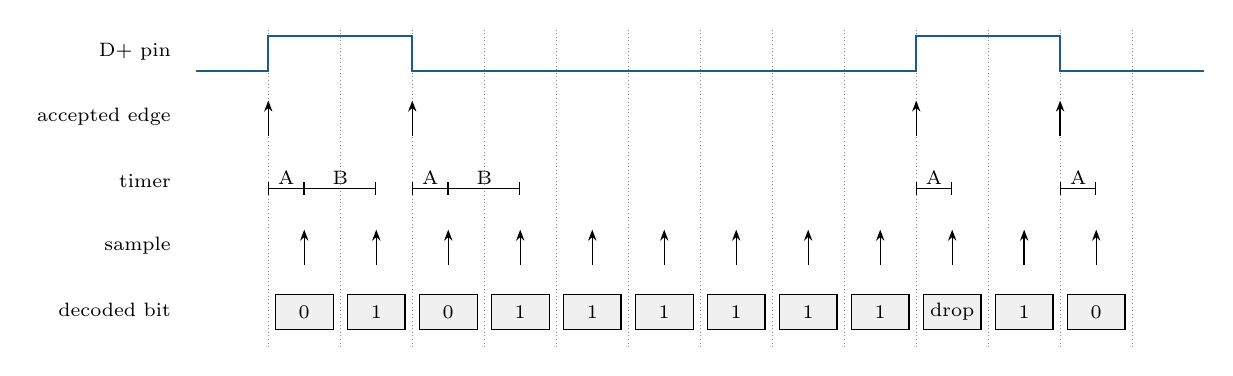
\begin{tikzpicture}[x=1mm,y=1mm]
\draw[densely dotted,line width=0.3pt,black!45] (36.14,1.00) -- (36.14,41.50);
\draw[densely dotted,line width=0.3pt,black!45] (45.29,1.00) -- (45.29,41.50);
\draw[densely dotted,line width=0.3pt,black!45] (54.43,1.00) -- (54.43,41.50);
\draw[densely dotted,line width=0.3pt,black!45] (63.57,1.00) -- (63.57,41.50);
\draw[densely dotted,line width=0.3pt,black!45] (72.71,1.00) -- (72.71,41.50);
\draw[densely dotted,line width=0.3pt,black!45] (81.86,1.00) -- (81.86,41.50);
\draw[densely dotted,line width=0.3pt,black!45] (91.00,1.00) -- (91.00,41.50);
\draw[densely dotted,line width=0.3pt,black!45] (100.14,1.00) -- (100.14,41.50);
\draw[densely dotted,line width=0.3pt,black!45] (109.29,1.00) -- (109.29,41.50);
\draw[densely dotted,line width=0.3pt,black!45] (118.43,1.00) -- (118.43,41.50);
\draw[densely dotted,line width=0.3pt,black!45] (127.57,1.00) -- (127.57,41.50);
\draw[densely dotted,line width=0.3pt,black!45] (136.71,1.00) -- (136.71,41.50);
\draw[densely dotted,line width=0.3pt,black!45] (145.86,1.00) -- (145.86,41.50);
\node[lbl,anchor=east] at (25.00,38.50) {D+ pin};
\draw[line width=0.7pt,accent] (27.00,36.00) -- (36.14,36.00) -- (36.14,40.50) -- (54.43,40.50) -- (54.43,36.00) -- (118.43,36.00) -- (118.43,40.50) -- (136.71,40.50) -- (136.71,36.00) -- (155.00,36.00);
\node[lbl,anchor=east] at (25.00,30.30) {accepted edge};
\draw[-{Stealth[length=1.4mm]},line width=0.5pt] (36.14,27.80) -- (36.14,32.30);
\draw[-{Stealth[length=1.4mm]},line width=0.5pt] (54.43,27.80) -- (54.43,32.30);
\draw[-{Stealth[length=1.4mm]},line width=0.5pt] (118.43,27.80) -- (118.43,32.30);
\draw[-{Stealth[length=1.4mm]},line width=0.5pt] (136.71,27.80) -- (136.71,32.30);
\node[lbl,anchor=east] at (25.00,22.10) {timer};
\draw[|-|,line width=0.4pt] (36.14,21.10) -- (40.71,21.10);
\node[lbl,anchor=south,inner sep=0.6pt] at (38.43,21.30) {A};
\draw[|-|,line width=0.4pt] (40.71,21.10) -- (49.86,21.10);
\node[lbl,anchor=south,inner sep=0.6pt] at (45.29,21.30) {B};
\draw[|-|,line width=0.4pt] (54.43,21.10) -- (59.00,21.10);
\node[lbl,anchor=south,inner sep=0.6pt] at (56.71,21.30) {A};
\draw[|-|,line width=0.4pt] (59.00,21.10) -- (68.14,21.10);
\node[lbl,anchor=south,inner sep=0.6pt] at (63.57,21.30) {B};
\draw[|-|,line width=0.4pt] (118.43,21.10) -- (123.00,21.10);
\node[lbl,anchor=south,inner sep=0.6pt] at (120.71,21.30) {A};
\draw[|-|,line width=0.4pt] (136.71,21.10) -- (141.29,21.10);
\node[lbl,anchor=south,inner sep=0.6pt] at (139.00,21.30) {A};
\node[lbl,anchor=east] at (25.00,13.90) {sample};
\draw[-{Stealth[length=1.4mm]},line width=0.5pt] (40.71,11.40) -- (40.71,15.90);
\draw[-{Stealth[length=1.4mm]},line width=0.5pt] (49.86,11.40) -- (49.86,15.90);
\draw[-{Stealth[length=1.4mm]},line width=0.5pt] (59.00,11.40) -- (59.00,15.90);
\draw[-{Stealth[length=1.4mm]},line width=0.5pt] (68.14,11.40) -- (68.14,15.90);
\draw[-{Stealth[length=1.4mm]},line width=0.5pt] (77.29,11.40) -- (77.29,15.90);
\draw[-{Stealth[length=1.4mm]},line width=0.5pt] (86.43,11.40) -- (86.43,15.90);
\draw[-{Stealth[length=1.4mm]},line width=0.5pt] (95.57,11.40) -- (95.57,15.90);
\draw[-{Stealth[length=1.4mm]},line width=0.5pt] (104.71,11.40) -- (104.71,15.90);
\draw[-{Stealth[length=1.4mm]},line width=0.5pt] (113.86,11.40) -- (113.86,15.90);
\draw[-{Stealth[length=1.4mm]},line width=0.5pt] (123.00,11.40) -- (123.00,15.90);
\draw[-{Stealth[length=1.4mm]},line width=0.5pt] (132.14,11.40) -- (132.14,15.90);
\draw[-{Stealth[length=1.4mm]},line width=0.5pt] (141.29,11.40) -- (141.29,15.90);
\node[lbl,anchor=east] at (25.00,5.70) {decoded bit};
\draw[line width=0.4pt,fill=fillD] (37.06,3.20) rectangle (44.37,7.70);
\node[lbl,inner sep=0pt] at (40.71,5.45) {0};
\draw[line width=0.4pt,fill=fillD] (46.20,3.20) rectangle (53.51,7.70);
\node[lbl,inner sep=0pt] at (49.86,5.45) {1};
\draw[line width=0.4pt,fill=fillD] (55.34,3.20) rectangle (62.66,7.70);
\node[lbl,inner sep=0pt] at (59.00,5.45) {0};
\draw[line width=0.4pt,fill=fillD] (64.49,3.20) rectangle (71.80,7.70);
\node[lbl,inner sep=0pt] at (68.14,5.45) {1};
\draw[line width=0.4pt,fill=fillD] (73.63,3.20) rectangle (80.94,7.70);
\node[lbl,inner sep=0pt] at (77.29,5.45) {1};
\draw[line width=0.4pt,fill=fillD] (82.77,3.20) rectangle (90.09,7.70);
\node[lbl,inner sep=0pt] at (86.43,5.45) {1};
\draw[line width=0.4pt,fill=fillD] (91.91,3.20) rectangle (99.23,7.70);
\node[lbl,inner sep=0pt] at (95.57,5.45) {1};
\draw[line width=0.4pt,fill=fillD] (101.06,3.20) rectangle (108.37,7.70);
\node[lbl,inner sep=0pt] at (104.71,5.45) {1};
\draw[line width=0.4pt,fill=fillD] (110.20,3.20) rectangle (117.51,7.70);
\node[lbl,inner sep=0pt] at (113.86,5.45) {1};
\draw[line width=0.4pt,fill=fillD] (119.34,3.20) rectangle (126.66,7.70);
\node[lbl,inner sep=0pt] at (123.00,5.45) {drop};
\draw[line width=0.4pt,fill=fillD] (128.49,3.20) rectangle (135.80,7.70);
\node[lbl,inner sep=0pt] at (132.14,5.45) {1};
\draw[line width=0.4pt,fill=fillD] (137.63,3.20) rectangle (144.94,7.70);
\node[lbl,inner sep=0pt] at (141.29,5.45) {0};
\end{tikzpicture}
\caption{USB low-speed receive. Bit 9 is the stuffed bit after six ones.}
\label{fig:usbrx}
\end{figure}

\textbf{Transmit.} \reg{TXEN}; B = 40; \reg{LCENC} = NRZI; \reg{LIM} = 6; complementary output on the second
pin; output enable while busy (\reg{OEM} = 2), so that the pull resistors give the idle state. The cell inserts the stuffed bit. With \reg{EOP} set the cell ends the packet itself: both pins are low for two bit periods after the last bit, then the pins are released. Without \reg{EOP}, firmware does the same by setting \reg{LOW2} for two bit times.


\begin{figure}[H]
\centering
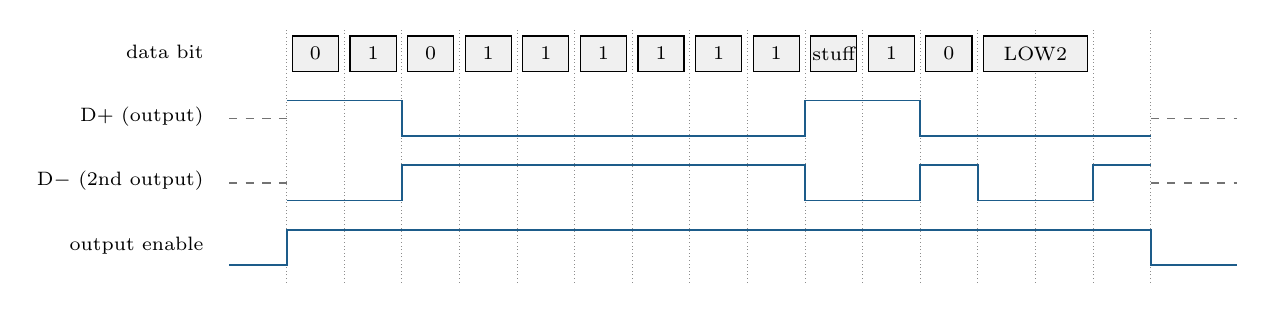
\begin{tikzpicture}[x=1mm,y=1mm]
\draw[densely dotted,line width=0.3pt,black!45] (34.31,1.00) -- (34.31,33.30);
\draw[densely dotted,line width=0.3pt,black!45] (41.63,1.00) -- (41.63,33.30);
\draw[densely dotted,line width=0.3pt,black!45] (48.94,1.00) -- (48.94,33.30);
\draw[densely dotted,line width=0.3pt,black!45] (56.26,1.00) -- (56.26,33.30);
\draw[densely dotted,line width=0.3pt,black!45] (63.57,1.00) -- (63.57,33.30);
\draw[densely dotted,line width=0.3pt,black!45] (70.89,1.00) -- (70.89,33.30);
\draw[densely dotted,line width=0.3pt,black!45] (78.20,1.00) -- (78.20,33.30);
\draw[densely dotted,line width=0.3pt,black!45] (85.51,1.00) -- (85.51,33.30);
\draw[densely dotted,line width=0.3pt,black!45] (92.83,1.00) -- (92.83,33.30);
\draw[densely dotted,line width=0.3pt,black!45] (100.14,1.00) -- (100.14,33.30);
\draw[densely dotted,line width=0.3pt,black!45] (107.46,1.00) -- (107.46,33.30);
\draw[densely dotted,line width=0.3pt,black!45] (114.77,1.00) -- (114.77,33.30);
\draw[densely dotted,line width=0.3pt,black!45] (122.09,1.00) -- (122.09,33.30);
\draw[densely dotted,line width=0.3pt,black!45] (129.40,1.00) -- (129.40,33.30);
\draw[densely dotted,line width=0.3pt,black!45] (136.71,1.00) -- (136.71,33.30);
\draw[densely dotted,line width=0.3pt,black!45] (144.03,1.00) -- (144.03,33.30);
\node[lbl,anchor=east] at (25.00,30.30) {data bit};
\draw[line width=0.4pt,fill=fillD] (35.05,27.80) rectangle (40.90,32.30);
\node[lbl,inner sep=0pt] at (37.97,30.05) {0};
\draw[line width=0.4pt,fill=fillD] (42.36,27.80) rectangle (48.21,32.30);
\node[lbl,inner sep=0pt] at (45.29,30.05) {1};
\draw[line width=0.4pt,fill=fillD] (49.67,27.80) rectangle (55.53,32.30);
\node[lbl,inner sep=0pt] at (52.60,30.05) {0};
\draw[line width=0.4pt,fill=fillD] (56.99,27.80) rectangle (62.84,32.30);
\node[lbl,inner sep=0pt] at (59.91,30.05) {1};
\draw[line width=0.4pt,fill=fillD] (64.30,27.80) rectangle (70.15,32.30);
\node[lbl,inner sep=0pt] at (67.23,30.05) {1};
\draw[line width=0.4pt,fill=fillD] (71.62,27.80) rectangle (77.47,32.30);
\node[lbl,inner sep=0pt] at (74.54,30.05) {1};
\draw[line width=0.4pt,fill=fillD] (78.93,27.80) rectangle (84.78,32.30);
\node[lbl,inner sep=0pt] at (81.86,30.05) {1};
\draw[line width=0.4pt,fill=fillD] (86.25,27.80) rectangle (92.10,32.30);
\node[lbl,inner sep=0pt] at (89.17,30.05) {1};
\draw[line width=0.4pt,fill=fillD] (93.56,27.80) rectangle (99.41,32.30);
\node[lbl,inner sep=0pt] at (96.49,30.05) {1};
\draw[line width=0.4pt,fill=fillD] (100.87,27.80) rectangle (106.73,32.30);
\node[lbl,inner sep=0pt] at (103.80,30.05) {stuff};
\draw[line width=0.4pt,fill=fillD] (108.19,27.80) rectangle (114.04,32.30);
\node[lbl,inner sep=0pt] at (111.11,30.05) {1};
\draw[line width=0.4pt,fill=fillD] (115.50,27.80) rectangle (121.35,32.30);
\node[lbl,inner sep=0pt] at (118.43,30.05) {0};
\draw[line width=0.4pt,fill=fillD] (122.82,27.80) rectangle (135.98,32.30);
\node[lbl,inner sep=0pt] at (129.40,30.05) {LOW2};
\node[lbl,anchor=east] at (25.00,22.10) {D+ (output)};
\draw[dashed,line width=0.5pt,black!55] (27.00,21.85) -- (34.31,21.85);
\draw[line width=0.7pt,accent] (34.31,24.10) -- (48.94,24.10) -- (48.94,19.60) -- (100.14,19.60) -- (100.14,24.10) -- (114.77,24.10) -- (114.77,19.60) -- (122.09,19.60) -- (122.09,19.60) -- (136.71,19.60) -- (136.71,19.60) -- (144.03,19.60);
\draw[dashed,line width=0.5pt,black!55] (144.03,21.85) -- (155.00,21.85);
\node[lbl,anchor=east] at (25.00,13.90) {D$-$ (2nd output)};
\draw[dashed,line width=0.5pt,black!55] (27.00,13.65) -- (34.31,13.65);
\draw[line width=0.7pt,accent] (34.31,11.40) -- (48.94,11.40) -- (48.94,15.90) -- (100.14,15.90) -- (100.14,11.40) -- (114.77,11.40) -- (114.77,15.90) -- (122.09,15.90) -- (122.09,11.40) -- (136.71,11.40) -- (136.71,15.90) -- (144.03,15.90);
\draw[dashed,line width=0.5pt,black!55] (144.03,13.65) -- (155.00,13.65);
\node[lbl,anchor=east] at (25.00,5.70) {output enable};
\draw[line width=0.7pt,accent] (27.00,3.20) -- (34.31,3.20) -- (34.31,7.70) -- (144.03,7.70) -- (144.03,3.20) -- (155.00,3.20);
\end{tikzpicture}
\caption{USB low-speed transmit of the same bits, followed by the end of packet and one bit of idle state.}
\label{fig:usbtx}
\end{figure}

\subsection{10BASE-T}

\textbf{Receive.} Time unit = both edges of the source clock, which gives 12 units per bit; \reg{EDGE} = both,
accepted only while waiting; \reg{STOP} = after each sample; A = 9 (0.75 bit); B = 24 as end-of-frame timeout;
\reg{LCDEC} = inverted level; match on the start-of-frame delimiter. Each mid-bit edge starts the timer. It
expires in the first half of the next bit, where the level is the inverse of that bit. The edge at the bit
boundary, if there is one, falls inside the timer interval and is ignored.


\begin{figure}[H]
\centering
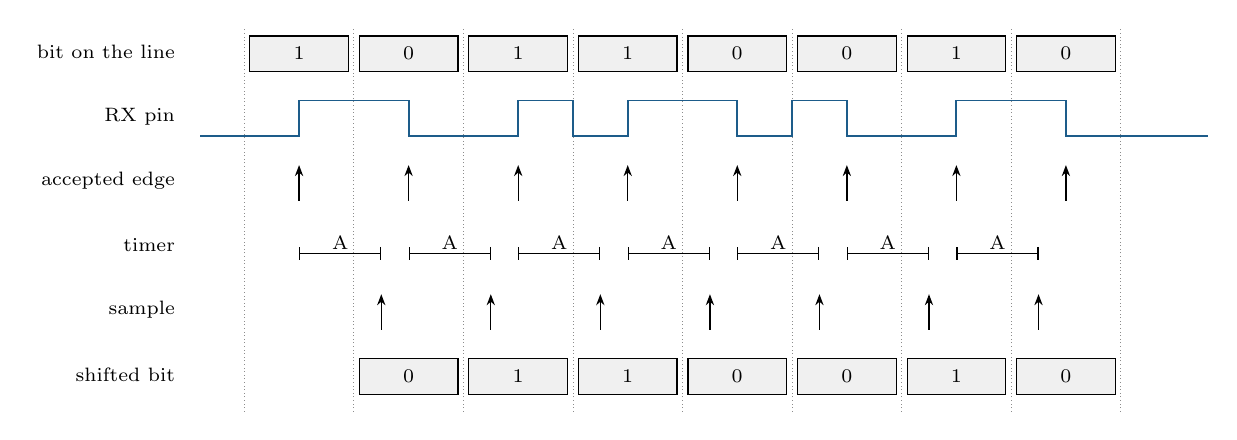
\begin{tikzpicture}[x=1mm,y=1mm]
\draw[densely dotted,line width=0.3pt,black!45] (32.57,1.00) -- (32.57,49.70);
\draw[densely dotted,line width=0.3pt,black!45] (46.48,1.00) -- (46.48,49.70);
\draw[densely dotted,line width=0.3pt,black!45] (60.39,1.00) -- (60.39,49.70);
\draw[densely dotted,line width=0.3pt,black!45] (74.30,1.00) -- (74.30,49.70);
\draw[densely dotted,line width=0.3pt,black!45] (88.22,1.00) -- (88.22,49.70);
\draw[densely dotted,line width=0.3pt,black!45] (102.13,1.00) -- (102.13,49.70);
\draw[densely dotted,line width=0.3pt,black!45] (116.04,1.00) -- (116.04,49.70);
\draw[densely dotted,line width=0.3pt,black!45] (129.96,1.00) -- (129.96,49.70);
\draw[densely dotted,line width=0.3pt,black!45] (143.87,1.00) -- (143.87,49.70);
\node[lbl,anchor=east] at (25.00,46.70) {bit on the line};
\draw[line width=0.4pt,fill=fillD] (33.26,44.20) rectangle (45.78,48.70);
\node[lbl,inner sep=0pt] at (39.52,46.45) {1};
\draw[line width=0.4pt,fill=fillD] (47.17,44.20) rectangle (59.70,48.70);
\node[lbl,inner sep=0pt] at (53.43,46.45) {0};
\draw[line width=0.4pt,fill=fillD] (61.09,44.20) rectangle (73.61,48.70);
\node[lbl,inner sep=0pt] at (67.35,46.45) {1};
\draw[line width=0.4pt,fill=fillD] (75.00,44.20) rectangle (87.52,48.70);
\node[lbl,inner sep=0pt] at (81.26,46.45) {1};
\draw[line width=0.4pt,fill=fillD] (88.91,44.20) rectangle (101.43,48.70);
\node[lbl,inner sep=0pt] at (95.17,46.45) {0};
\draw[line width=0.4pt,fill=fillD] (102.83,44.20) rectangle (115.35,48.70);
\node[lbl,inner sep=0pt] at (109.09,46.45) {0};
\draw[line width=0.4pt,fill=fillD] (116.74,44.20) rectangle (129.26,48.70);
\node[lbl,inner sep=0pt] at (123.00,46.45) {1};
\draw[line width=0.4pt,fill=fillD] (130.65,44.20) rectangle (143.17,48.70);
\node[lbl,inner sep=0pt] at (136.91,46.45) {0};
\node[lbl,anchor=east] at (25.00,38.50) {RX pin};
\draw[line width=0.7pt,accent] (27.00,36.00) -- (32.57,36.00) -- (32.57,36.00) -- (39.52,36.00) -- (39.52,40.50) -- (46.48,40.50) -- (46.48,40.50) -- (53.43,40.50) -- (53.43,36.00) -- (60.39,36.00) -- (60.39,36.00) -- (67.35,36.00) -- (67.35,40.50) -- (74.30,40.50) -- (74.30,36.00) -- (81.26,36.00) -- (81.26,40.50) -- (88.22,40.50) -- (88.22,40.50) -- (95.17,40.50) -- (95.17,36.00) -- (102.13,36.00) -- (102.13,40.50) -- (109.09,40.50) -- (109.09,36.00) -- (116.04,36.00) -- (116.04,36.00) -- (123.00,36.00) -- (123.00,40.50) -- (129.96,40.50) -- (129.96,40.50) -- (136.91,40.50) -- (136.91,36.00) -- (143.87,36.00) -- (143.87,36.00) -- (155.00,36.00);
\node[lbl,anchor=east] at (25.00,30.30) {accepted edge};
\draw[-{Stealth[length=1.4mm]},line width=0.5pt] (39.52,27.80) -- (39.52,32.30);
\draw[-{Stealth[length=1.4mm]},line width=0.5pt] (53.43,27.80) -- (53.43,32.30);
\draw[-{Stealth[length=1.4mm]},line width=0.5pt] (67.35,27.80) -- (67.35,32.30);
\draw[-{Stealth[length=1.4mm]},line width=0.5pt] (81.26,27.80) -- (81.26,32.30);
\draw[-{Stealth[length=1.4mm]},line width=0.5pt] (95.17,27.80) -- (95.17,32.30);
\draw[-{Stealth[length=1.4mm]},line width=0.5pt] (109.09,27.80) -- (109.09,32.30);
\draw[-{Stealth[length=1.4mm]},line width=0.5pt] (123.00,27.80) -- (123.00,32.30);
\draw[-{Stealth[length=1.4mm]},line width=0.5pt] (136.91,27.80) -- (136.91,32.30);
\node[lbl,anchor=east] at (25.00,22.10) {timer};
\draw[|-|,line width=0.4pt] (39.52,21.10) -- (49.96,21.10);
\node[lbl,anchor=south,inner sep=0.6pt] at (44.74,21.30) {A};
\draw[|-|,line width=0.4pt] (53.43,21.10) -- (63.87,21.10);
\node[lbl,anchor=south,inner sep=0.6pt] at (58.65,21.30) {A};
\draw[|-|,line width=0.4pt] (67.35,21.10) -- (77.78,21.10);
\node[lbl,anchor=south,inner sep=0.6pt] at (72.57,21.30) {A};
\draw[|-|,line width=0.4pt] (81.26,21.10) -- (91.70,21.10);
\node[lbl,anchor=south,inner sep=0.6pt] at (86.48,21.30) {A};
\draw[|-|,line width=0.4pt] (95.17,21.10) -- (105.61,21.10);
\node[lbl,anchor=south,inner sep=0.6pt] at (100.39,21.30) {A};
\draw[|-|,line width=0.4pt] (109.09,21.10) -- (119.52,21.10);
\node[lbl,anchor=south,inner sep=0.6pt] at (114.30,21.30) {A};
\draw[|-|,line width=0.4pt] (123.00,21.10) -- (133.43,21.10);
\node[lbl,anchor=south,inner sep=0.6pt] at (128.22,21.30) {A};
\node[lbl,anchor=east] at (25.00,13.90) {sample};
\draw[-{Stealth[length=1.4mm]},line width=0.5pt] (49.96,11.40) -- (49.96,15.90);
\draw[-{Stealth[length=1.4mm]},line width=0.5pt] (63.87,11.40) -- (63.87,15.90);
\draw[-{Stealth[length=1.4mm]},line width=0.5pt] (77.78,11.40) -- (77.78,15.90);
\draw[-{Stealth[length=1.4mm]},line width=0.5pt] (91.70,11.40) -- (91.70,15.90);
\draw[-{Stealth[length=1.4mm]},line width=0.5pt] (105.61,11.40) -- (105.61,15.90);
\draw[-{Stealth[length=1.4mm]},line width=0.5pt] (119.52,11.40) -- (119.52,15.90);
\draw[-{Stealth[length=1.4mm]},line width=0.5pt] (133.43,11.40) -- (133.43,15.90);
\node[lbl,anchor=east] at (25.00,5.70) {shifted bit};
\draw[line width=0.4pt,fill=fillD] (47.17,3.20) rectangle (59.70,7.70);
\node[lbl,inner sep=0pt] at (53.43,5.45) {0};
\draw[line width=0.4pt,fill=fillD] (61.09,3.20) rectangle (73.61,7.70);
\node[lbl,inner sep=0pt] at (67.35,5.45) {1};
\draw[line width=0.4pt,fill=fillD] (75.00,3.20) rectangle (87.52,7.70);
\node[lbl,inner sep=0pt] at (81.26,5.45) {1};
\draw[line width=0.4pt,fill=fillD] (88.91,3.20) rectangle (101.43,7.70);
\node[lbl,inner sep=0pt] at (95.17,5.45) {0};
\draw[line width=0.4pt,fill=fillD] (102.83,3.20) rectangle (115.35,7.70);
\node[lbl,inner sep=0pt] at (109.09,5.45) {0};
\draw[line width=0.4pt,fill=fillD] (116.74,3.20) rectangle (129.26,7.70);
\node[lbl,inner sep=0pt] at (123.00,5.45) {1};
\draw[line width=0.4pt,fill=fillD] (130.65,3.20) rectangle (143.17,7.70);
\node[lbl,inner sep=0pt] at (136.91,5.45) {0};
\end{tikzpicture}
\caption{10BASE-T receive of Manchester-coded bits. The first bit shown belongs to the preamble and is not decoded.}
\label{fig:ethrx}
\end{figure}

\textbf{Transmit.} \reg{TXEN}; \reg{TWOPH} with B = 3 (half a bit); \reg{LCENC} = Manchester;
complementary output; \reg{IDLE} = low on both pins after the frame. Transmit needs a clock within the tolerance of the standard, so it runs from the external 60\,MHz clock only.


\begin{figure}[H]
\centering
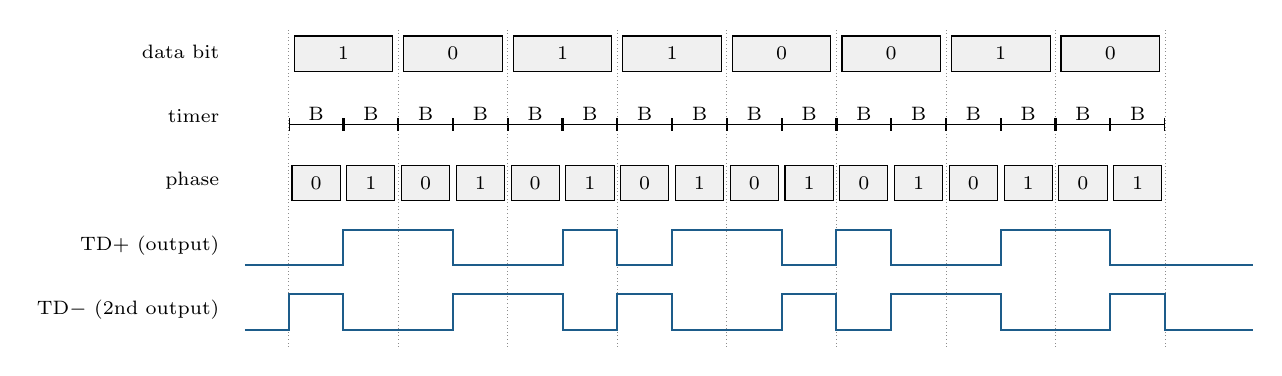
\begin{tikzpicture}[x=1mm,y=1mm]
\draw[densely dotted,line width=0.3pt,black!45] (32.57,1.00) -- (32.57,41.50);
\draw[densely dotted,line width=0.3pt,black!45] (46.48,1.00) -- (46.48,41.50);
\draw[densely dotted,line width=0.3pt,black!45] (60.39,1.00) -- (60.39,41.50);
\draw[densely dotted,line width=0.3pt,black!45] (74.30,1.00) -- (74.30,41.50);
\draw[densely dotted,line width=0.3pt,black!45] (88.22,1.00) -- (88.22,41.50);
\draw[densely dotted,line width=0.3pt,black!45] (102.13,1.00) -- (102.13,41.50);
\draw[densely dotted,line width=0.3pt,black!45] (116.04,1.00) -- (116.04,41.50);
\draw[densely dotted,line width=0.3pt,black!45] (129.96,1.00) -- (129.96,41.50);
\draw[densely dotted,line width=0.3pt,black!45] (143.87,1.00) -- (143.87,41.50);
\node[lbl,anchor=east] at (25.00,38.50) {data bit};
\draw[line width=0.4pt,fill=fillD] (33.26,36.00) rectangle (45.78,40.50);
\node[lbl,inner sep=0pt] at (39.52,38.25) {1};
\draw[line width=0.4pt,fill=fillD] (47.17,36.00) rectangle (59.70,40.50);
\node[lbl,inner sep=0pt] at (53.43,38.25) {0};
\draw[line width=0.4pt,fill=fillD] (61.09,36.00) rectangle (73.61,40.50);
\node[lbl,inner sep=0pt] at (67.35,38.25) {1};
\draw[line width=0.4pt,fill=fillD] (75.00,36.00) rectangle (87.52,40.50);
\node[lbl,inner sep=0pt] at (81.26,38.25) {1};
\draw[line width=0.4pt,fill=fillD] (88.91,36.00) rectangle (101.43,40.50);
\node[lbl,inner sep=0pt] at (95.17,38.25) {0};
\draw[line width=0.4pt,fill=fillD] (102.83,36.00) rectangle (115.35,40.50);
\node[lbl,inner sep=0pt] at (109.09,38.25) {0};
\draw[line width=0.4pt,fill=fillD] (116.74,36.00) rectangle (129.26,40.50);
\node[lbl,inner sep=0pt] at (123.00,38.25) {1};
\draw[line width=0.4pt,fill=fillD] (130.65,36.00) rectangle (143.17,40.50);
\node[lbl,inner sep=0pt] at (136.91,38.25) {0};
\node[lbl,anchor=east] at (25.00,30.30) {timer};
\draw[|-|,line width=0.4pt] (32.57,29.30) -- (39.52,29.30);
\node[lbl,anchor=south,inner sep=0.6pt] at (36.04,29.50) {B};
\draw[|-|,line width=0.4pt] (39.52,29.30) -- (46.48,29.30);
\node[lbl,anchor=south,inner sep=0.6pt] at (43.00,29.50) {B};
\draw[|-|,line width=0.4pt] (46.48,29.30) -- (53.43,29.30);
\node[lbl,anchor=south,inner sep=0.6pt] at (49.96,29.50) {B};
\draw[|-|,line width=0.4pt] (53.43,29.30) -- (60.39,29.30);
\node[lbl,anchor=south,inner sep=0.6pt] at (56.91,29.50) {B};
\draw[|-|,line width=0.4pt] (60.39,29.30) -- (67.35,29.30);
\node[lbl,anchor=south,inner sep=0.6pt] at (63.87,29.50) {B};
\draw[|-|,line width=0.4pt] (67.35,29.30) -- (74.30,29.30);
\node[lbl,anchor=south,inner sep=0.6pt] at (70.83,29.50) {B};
\draw[|-|,line width=0.4pt] (74.30,29.30) -- (81.26,29.30);
\node[lbl,anchor=south,inner sep=0.6pt] at (77.78,29.50) {B};
\draw[|-|,line width=0.4pt] (81.26,29.30) -- (88.22,29.30);
\node[lbl,anchor=south,inner sep=0.6pt] at (84.74,29.50) {B};
\draw[|-|,line width=0.4pt] (88.22,29.30) -- (95.17,29.30);
\node[lbl,anchor=south,inner sep=0.6pt] at (91.70,29.50) {B};
\draw[|-|,line width=0.4pt] (95.17,29.30) -- (102.13,29.30);
\node[lbl,anchor=south,inner sep=0.6pt] at (98.65,29.50) {B};
\draw[|-|,line width=0.4pt] (102.13,29.30) -- (109.09,29.30);
\node[lbl,anchor=south,inner sep=0.6pt] at (105.61,29.50) {B};
\draw[|-|,line width=0.4pt] (109.09,29.30) -- (116.04,29.30);
\node[lbl,anchor=south,inner sep=0.6pt] at (112.57,29.50) {B};
\draw[|-|,line width=0.4pt] (116.04,29.30) -- (123.00,29.30);
\node[lbl,anchor=south,inner sep=0.6pt] at (119.52,29.50) {B};
\draw[|-|,line width=0.4pt] (123.00,29.30) -- (129.96,29.30);
\node[lbl,anchor=south,inner sep=0.6pt] at (126.48,29.50) {B};
\draw[|-|,line width=0.4pt] (129.96,29.30) -- (136.91,29.30);
\node[lbl,anchor=south,inner sep=0.6pt] at (133.43,29.50) {B};
\draw[|-|,line width=0.4pt] (136.91,29.30) -- (143.87,29.30);
\node[lbl,anchor=south,inner sep=0.6pt] at (140.39,29.50) {B};
\node[lbl,anchor=east] at (25.00,22.10) {phase};
\draw[line width=0.4pt,fill=fillD] (32.98,19.60) rectangle (39.10,24.10);
\node[lbl,inner sep=0pt] at (36.04,21.85) {0};
\draw[line width=0.4pt,fill=fillD] (39.94,19.60) rectangle (46.06,24.10);
\node[lbl,inner sep=0pt] at (43.00,21.85) {1};
\draw[line width=0.4pt,fill=fillD] (46.90,19.60) rectangle (53.02,24.10);
\node[lbl,inner sep=0pt] at (49.96,21.85) {0};
\draw[line width=0.4pt,fill=fillD] (53.85,19.60) rectangle (59.97,24.10);
\node[lbl,inner sep=0pt] at (56.91,21.85) {1};
\draw[line width=0.4pt,fill=fillD] (60.81,19.60) rectangle (66.93,24.10);
\node[lbl,inner sep=0pt] at (63.87,21.85) {0};
\draw[line width=0.4pt,fill=fillD] (67.77,19.60) rectangle (73.89,24.10);
\node[lbl,inner sep=0pt] at (70.83,21.85) {1};
\draw[line width=0.4pt,fill=fillD] (74.72,19.60) rectangle (80.84,24.10);
\node[lbl,inner sep=0pt] at (77.78,21.85) {0};
\draw[line width=0.4pt,fill=fillD] (81.68,19.60) rectangle (87.80,24.10);
\node[lbl,inner sep=0pt] at (84.74,21.85) {1};
\draw[line width=0.4pt,fill=fillD] (88.63,19.60) rectangle (94.76,24.10);
\node[lbl,inner sep=0pt] at (91.70,21.85) {0};
\draw[line width=0.4pt,fill=fillD] (95.59,19.60) rectangle (101.71,24.10);
\node[lbl,inner sep=0pt] at (98.65,21.85) {1};
\draw[line width=0.4pt,fill=fillD] (102.55,19.60) rectangle (108.67,24.10);
\node[lbl,inner sep=0pt] at (105.61,21.85) {0};
\draw[line width=0.4pt,fill=fillD] (109.50,19.60) rectangle (115.63,24.10);
\node[lbl,inner sep=0pt] at (112.57,21.85) {1};
\draw[line width=0.4pt,fill=fillD] (116.46,19.60) rectangle (122.58,24.10);
\node[lbl,inner sep=0pt] at (119.52,21.85) {0};
\draw[line width=0.4pt,fill=fillD] (123.42,19.60) rectangle (129.54,24.10);
\node[lbl,inner sep=0pt] at (126.48,21.85) {1};
\draw[line width=0.4pt,fill=fillD] (130.37,19.60) rectangle (136.50,24.10);
\node[lbl,inner sep=0pt] at (133.43,21.85) {0};
\draw[line width=0.4pt,fill=fillD] (137.33,19.60) rectangle (143.45,24.10);
\node[lbl,inner sep=0pt] at (140.39,21.85) {1};
\node[lbl,anchor=east] at (25.00,13.90) {TD+ (output)};
\draw[line width=0.7pt,accent] (27.00,11.40) -- (32.57,11.40) -- (32.57,11.40) -- (39.52,11.40) -- (39.52,15.90) -- (46.48,15.90) -- (46.48,15.90) -- (53.43,15.90) -- (53.43,11.40) -- (60.39,11.40) -- (60.39,11.40) -- (67.35,11.40) -- (67.35,15.90) -- (74.30,15.90) -- (74.30,11.40) -- (81.26,11.40) -- (81.26,15.90) -- (88.22,15.90) -- (88.22,15.90) -- (95.17,15.90) -- (95.17,11.40) -- (102.13,11.40) -- (102.13,15.90) -- (109.09,15.90) -- (109.09,11.40) -- (116.04,11.40) -- (116.04,11.40) -- (123.00,11.40) -- (123.00,15.90) -- (129.96,15.90) -- (129.96,15.90) -- (136.91,15.90) -- (136.91,11.40) -- (143.87,11.40) -- (143.87,11.40) -- (155.00,11.40);
\node[lbl,anchor=east] at (25.00,5.70) {TD$-$ (2nd output)};
\draw[line width=0.7pt,accent] (27.00,3.20) -- (32.57,3.20) -- (32.57,7.70) -- (39.52,7.70) -- (39.52,3.20) -- (46.48,3.20) -- (46.48,3.20) -- (53.43,3.20) -- (53.43,7.70) -- (60.39,7.70) -- (60.39,7.70) -- (67.35,7.70) -- (67.35,3.20) -- (74.30,3.20) -- (74.30,7.70) -- (81.26,7.70) -- (81.26,3.20) -- (88.22,3.20) -- (88.22,3.20) -- (95.17,3.20) -- (95.17,7.70) -- (102.13,7.70) -- (102.13,3.20) -- (109.09,3.20) -- (109.09,7.70) -- (116.04,7.70) -- (116.04,7.70) -- (123.00,7.70) -- (123.00,3.20) -- (129.96,3.20) -- (129.96,3.20) -- (136.91,3.20) -- (136.91,7.70) -- (143.87,7.70) -- (143.87,3.20) -- (155.00,3.20);
\end{tikzpicture}
\caption{10BASE-T transmit of the same bits. Both outputs are low before and after the frame.}
\label{fig:ethtx}
\end{figure}

\section{Clocking}\label{sec:clock}

The chip runs from one of two clock sources: an external clock, as supplied in the competition, or an internal
relaxation oscillator. The internal oscillator is not as accurate as a crystal. Untrimmed it may be off by
$\pm 30\,\%$, and no trim value is stored: the host trims it after each power-up. One clock serves the whole
chip, with separate dividers for the core and the peripherals.

\begin{figure}[!htb]
\centering
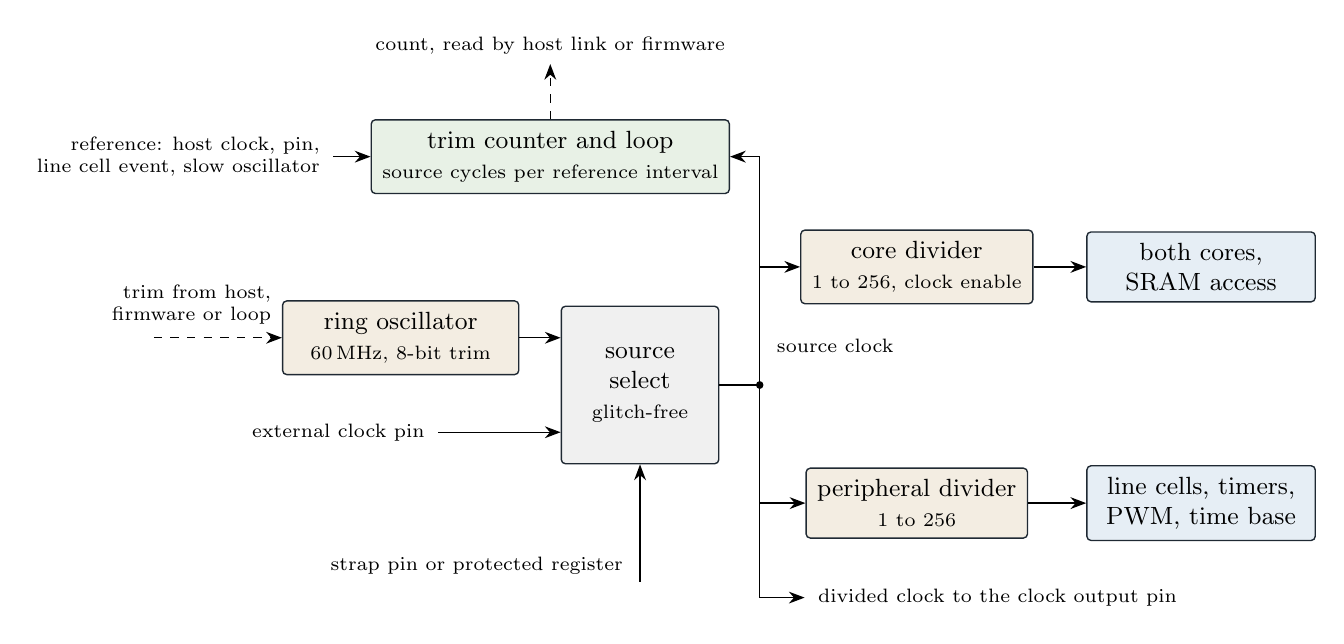
\begin{tikzpicture}[x=0.95mm,y=1mm]
  \node[blk,fill=fillB,minimum width=30mm] (osc) at (34,21) {ring oscillator\\ \scriptsize 60\,MHz, 8-bit trim};
  \node[blk,fill=fillD,minimum width=20mm,minimum height=20mm] (mux) at (66,15) {source\\ select\\ \scriptsize glitch-free};
  \draw[ar] (osc.east) -- ($(mux.west)+(0,6)$);
  \draw[ar] (39,9) -- ($(mux.west)+(0,-6)$);
  \node[lbl,anchor=east] at (38.5,9) {external clock pin};
  \draw[ar,dashed] (1,21) -- (osc.west);
  \node[lbl,anchor=south east,align=right] at (18,21.5) {trim from host,\\ firmware or loop};
  \draw[ar] (66,-10) -- (mux.south);
  \node[lbl,anchor=east] at (65,-8) {strap pin or protected register};
  \draw[line width=0.5pt] (mux.east) -- (82,15);
  \draw[line width=0.5pt] (82,-12) -- (82,44);
  \fill (82,15) circle (0.5);
  \node[blk,fill=fillB,minimum width=26mm] (cdiv) at (103,30) {core divider\\ \scriptsize 1 to 256, clock enable};
  \node[blk,fill=fillA,minimum width=29mm] (core) at (141,30) {both cores,\\ SRAM access};
  \node[blk,fill=fillB,minimum width=26mm] (pdiv) at (103,0) {peripheral divider\\ \scriptsize 1 to 256};
  \node[blk,fill=fillA,minimum width=29mm] (per) at (141,0) {line cells, timers,\\ PWM, time base};
  \draw[ar] (82,30) -- (cdiv.west);
  \draw[ar] (82,0) -- (pdiv.west);
  \draw[ar] (cdiv) -- (core);
  \draw[ar] (pdiv) -- (per);
  \node[blk,fill=fillC,minimum width=36mm] (cnt) at (54,44) {trim counter and loop\\ \scriptsize source cycles per reference interval};
  \draw[ar] (82,44) -- (cnt.east);
  \draw[ar] (25,44) -- (cnt.west);
  \node[lbl,anchor=east,align=right] at (24.5,44) {reference: host clock, pin,\\ line cell event, slow oscillator};
  \draw[ar,dashed] (cnt.north) -- ++(0,7) node[above,lbl]{count, read by host link or firmware};
  \draw[ar] (82,-12) -- (88,-12);
  \node[lbl,anchor=west] at (88.5,-12) {divided clock to the clock output pin};
  \node[lbl,anchor=west] at (83,20) {source clock};
\end{tikzpicture}
\caption{Clocking. Solid arrows are clocks and controls, dashed arrows show the trimming path.}
\label{fig:clock}
\end{figure}

\subsection{Clock sources}\label{sec:clksrc}

\begin{itemize}
\item \textbf{External clock.} Used directly. In the competition the RP2350 supplies it, at up to 60\,MHz.
10BASE-T runs from this source only.
\item \textbf{Internal oscillators.} One full-custom macro (\texttt{rpe\_clk\_analog}, 171.5 by 137\,$\mu$m)
with digital pins only: two enable inputs, an 8-bit trim bus and two clock outputs. It contains a
current-controlled ring oscillator for the system clock, a relaxation oscillator of about 100\,kHz and a
self-biased current reference that both use. There is no bandgap reference. The design files, the layout and
the report are in the folder \texttt{analog/} of the repository.
\item \textbf{Ring oscillator.} Five stages loaded with MOM capacitors and supplied by an 8-bit current DAC
(\reg{OSCTRIM}). Table~\ref{tab:oscsim} gives the values from the simulation of the extracted layout.
\item \textbf{Relaxation oscillator.} A dual-slope oscillator with a threshold derived from polysilicon
resistors and MOS capacitors as integrating capacitors. It is the reference of the trim loop
(\reg{REFSEL} = 3) and can serve as a slow clock for a sleep state; the digital part has no sleep state yet.
\item \textbf{Accuracy without a reference.} In the schematic simulation at a fixed trim value the ring
frequency rises from 50 to 83\,MHz between $-40$ and 125\,$^\circ$C and falls by 10\,\% between 1.08 and 1.32\,V.
The ring is therefore used with the trim loop. The relaxation oscillator changes by $\pm 1.5\,\%$ over the supply
range and by $+1.7$ to $-3.3\,\%$ over the temperature range in the schematic simulation, and by $-15$ to
$+17\,\%$ between the corners of table~\ref{tab:oscsim}. Its frequency on a given chip is not known in advance:
it is a reference after one measurement against an external signal (section~\ref{sec:trim}).
\item \textbf{Interaction.} Enabling the relaxation oscillator lowers the ring frequency by about 5\,\% (59.9 to
57.1\,MHz at the typical corner). With the loop running this is corrected by the trim value.
\item \textbf{Frequencies above 60\,MHz.} The logic is timed for a period of 16.67\,ns. With trim values above
about 155 at the typical corner the ring is faster than that. Firmware, the host and the loop target have to
keep the system clock at or below 60\,MHz. The reset value of \reg{OSCTRIM} gives at most 58.5\,MHz at the three
simulated corners. A chip that stops because the trim value is too high is restarted with the reset pin and
the strap low.
\item \textbf{Drafts up to 0.36} specified one relaxation oscillator at 15\,MHz and no ring oscillator. The
tests in this document that name 15\,MHz were run with the oscillator model \texttt{tb/osc\_model.v} at that
frequency. They have not been repeated with a model of the ring at 60\,MHz.
\item \textbf{Product.} The product has the internal oscillators only. The external clock input exists on the
competition chip.
\end{itemize}

\begin{table}[H]
\centering\small
\begin{tabularx}{\linewidth}{@{}Llll@{}}
\toprule
Value & typical, 1.20\,V, 25\,$^\circ$C & slow, 1.08\,V, 125\,$^\circ$C & fast, 1.32\,V, $-40\,^\circ$C \\
\midrule
Ring, \reg{OSCTRIM} = 0 & 15.8\,MHz & & \\
Ring, \reg{OSCTRIM} = 128 (reset value) & 52.8\,MHz & 53.0\,MHz & 58.5\,MHz \\
Ring, \reg{OSCTRIM} = 155 & 59.9\,MHz & 59.1\,MHz & 66.9\,MHz \\
Ring, \reg{OSCTRIM} = 255 & 83.8\,MHz & 78.1\,MHz & 96.9\,MHz \\
Ring, step of \reg{OSCTRIM} near 60\,MHz & 0.25\,MHz (0.4\,\%) & & \\
Relaxation oscillator & 98.5\,kHz & 83.6\,kHz & 115.5\,kHz \\
Supply current, ring at trim 155 & 61.5\,$\mu$A & 57.6\,$\mu$A & 78.4\,$\mu$A \\
Supply current, relaxation oscillator only & 4.1\,$\mu$A & 4.2\,$\mu$A & 5.1\,$\mu$A \\
Supply current, both disabled & 6\,nA & 69\,nA & 8\,nA \\
\bottomrule
\end{tabularx}
\caption{Oscillator macro: simulation of the extracted layout (ngspice, parasitic capacitances from Magic).
Source: \texttt{analog/results/clk\_macro\_pex.csv} and \texttt{clk\_macro\_pex\_trim.csv}. No value is measured
on silicon.}
\label{tab:oscsim}
\end{table}

With the ring trimmed to 60\,MHz the example settings in sections~\ref{sec:lcreg} and~\ref{sec:ex} apply to both
sources.

\subsection{Source selection and switching}

\begin{itemize}
\item \textbf{After reset} a strap pin selects the source on the competition chip. With the strap at its default
the chip starts on the external clock, so a faulty oscillator cannot stop it.
\item \textbf{At run time} the host link or firmware requests a switch through a register that is protected by
the same unlock sequence as the program-write enable.
\item \textbf{Glitch-free switch.} The old clock is stopped while it is low and the new clock is released on its
own edge, with synchronisers in both directions. The logic sees one long low phase and no short pulse.
\item \textbf{Presence check.} The switch starts only while the target clock is seen running. A request to switch to a missing clock is not executed, and the chip keeps running; the switch is made when the clock appears.
\item \textbf{The active oscillator cannot be switched off.} Clearing \reg{OSCEN} takes effect when the chip runs from the external clock.
\item \textbf{Status bits:} active source, oscillator running, trimmed.
\end{itemize}

\subsection{Dividers}

\begin{itemize}
\item \textbf{Core divider:} divides the source by any number from 1 to 256. It sets the rate of both cores and of their memory accesses. The reset value is 2: the cores run at 30\,MHz from a 60\,MHz source, while the line cells stay at 60\,MHz. The physical implementation is timed for this (section~\ref{sec:clk30}). A divider of 1 is allowed for a source clock of 30\,MHz or less. Its register follows the clock prescaler of the reduced AVR core and uses
the same unlock sequence.
\item \textbf{Peripheral divider:} an independent divider of the same kind for the line cells, timers, PWM and the time base. Each line cell keeps its own prescaler behind it.
\item Both divide the source clock, not each other, so changing the core speed does not change a bit rate.
\item \textbf{Implementation.} Each divider produces a clock enable on the source clock. There is one clock domain behind the source selection, and changing a divider cannot produce a short pulse.
\item \textbf{Bus strobes are qualified by the core enable,} so a peripheral that runs faster than the core does
not see one write twice.
\item The logic is timed for the 60\,MHz external clock. The ring oscillator can exceed this frequency
(section~\ref{sec:clksrc}); its reset trim value keeps it below.
\end{itemize}

\subsection{Trimming}\label{sec:trim}

\begin{itemize}
\item \textbf{Trim counter.} It counts source clock cycles over an interval set by a reference: a number of
periods of the host link clock, a signal on the reference pin, the relaxation oscillator, or the reference
event of a line cell. Only the ratio matters, so a slow reference is sufficient.
\item \textbf{At start-up, by the host.} The cores stay in reset. The host writes \reg{MEAS} through the host link, sends further clock periods as the reference, reads the count,
computes the trim value and writes it, and repeats this until the count is on target. This needs no firmware
and is the default start-up sequence. Alternatively the host sets \reg{LOOP} with the reference pin and waits.
\item \textbf{At run time, without an external reference,} the loop uses the relaxation oscillator. The
sequence: enable the relaxation oscillator (\reg{RELAXEN}), because it changes the ring frequency; trim the
ring against an external reference; select the relaxation oscillator as the reference (\reg{REFSEL} = 3) and
make one measurement; write the count to \reg{TRTGT}; set \reg{LOOP}. The count is about
609 per period of the relaxation oscillator at 60\,MHz and stops at 65\,535, so \reg{INT} is at most about 90.
The system clock then follows the relaxation oscillator, with its dependence on supply and temperature.
Without any reference and with the loop off, the ring runs free.
\item \textbf{At run time, with a reference,} the count is compared with a target register after every reference
interval, and the trim is stepped up or down by one. This loop is digital and reuses the trim counter. Firmware
can do the same by reading the count.
\item \textbf{Trim updates} are applied synchronously to the oscillator's own edge and in single steps, so a
change cannot produce a short period.
\end{itemize}

\subsection{Reference from a line}

A line can supply a reference that is more accurate than the free-running oscillator. This matters for USB,
where transmit has to be within $\pm 1.5\,\%$ and the host marks every millisecond on the bus.

\begin{itemize}
\item \textbf{Reference event.} Each line cell can produce a reference event, selected by a field in its
register set: an accepted edge, both pins low, or both pins low after the line was idle.
\item \textbf{Interval counter with window.} The trim counter measures the interval between two reference
events. A window register rejects intervals that are implausibly short or long, and an accepted measurement
sets an event flag.
\item \textbf{USB low-speed.} The cell detects both lines low. The host sends this as a keep-alive once per frame,
and it also ends every packet. The firmware needs the event of every end of packet for the answer time, so
the cell reports all of them, and the trim counter leaves out an event that comes not later than the target minus the window after the start of the interval (rule K7, section~\ref{sec:oscusb}). The interval is 15\,000 clock cycles, so one count is 0.007\,\%. The
cell can also report only ``both pins low after the line was idle''; a second receive cell on the same pins
with this setting is an alternative that was not needed.
\item \textbf{Use of the measurement.} The loop, or firmware, steps the trim by one after each accepted
interval. Between corrections and while the bus is suspended the oscillator runs free.
\item \textbf{Other lines.} A Manchester preamble or a known first character on a one-wire host link can be
measured the same way. For a UART partner the line cell's divider should be adjusted and not the system clock,
because the partner's own clock may be inaccurate.
\end{itemize}

\subsection{Host communication with an untrimmed clock}

\begin{itemize}
\item \textbf{Competition chip.} The host link is clocked by the host, and its accesses cross to the source
clock (rule L2). They work with any source clock that runs, trimmed or not. The clocking registers are
ordinary registers of the configuration page and are reached with the read and write commands. The host
clock has to stay below one eighth of the source clock (rule L2); with an untrimmed oscillator of 10\,MHz at the least\est{}
that is 1.25\,MHz.
\item \textbf{No source clock.} If the strap selects the oscillator and the oscillator does not run, the chip
does not start and the host link cannot reach a register. The strap pin is then set to the external clock. An
earlier draft kept copies of the clocking registers in the host clock domain for this case. They were dropped:
the strap covers it, and the copies needed a second crossing between the two clocks.
\item \textbf{Product, one-wire link.} The first contact has to be self-timed. The host sends a known first
character, and the chip measures its bit time before it decodes anything. The same measurement serves as the
reference for the first trim.
\end{itemize}

\subsection{Test and debug pins on the competition chip}

\begin{table}[H]
\centering\small
\begin{tabularx}{\linewidth}{@{}llL@{}}
\toprule
Pin & Direction & Function \\
\midrule
Clock source strap & input & Selects external clock or internal oscillator after reset \\
Reference & input & Reference signal for the trim counter, as an alternative to the host link clock \\
Clock output & output & Source clock divided by a selectable power of two, for measurement by the host or an instrument \\
Debug signal & output & One internal signal chosen by a register: a line cell's sample strobe or accepted edge, the clock enable of a core, a hold by the bus arbiter, or the core clock enable \\
\bottomrule
\end{tabularx}
\caption{Test and debug pins. They are taken from the plain input and output pins.}
\end{table}

The clock output lets the host measure the oscillator directly. The debug signal makes the timing of a line
cell visible next to the line itself, which is the main check of the protocol examples on the fabricated chip.

\subsection{Accuracy and protocols}

Directly after trimming, the error is at most one trim step, about 0.5\,\%\est. Afterwards the oscillator
drifts with temperature and supply. A drift of 1 to 2\,\% over the full temperature range is expected\est; this
is open until the oscillator has been simulated.

\begin{table}[H]
\centering\small
\begin{tabularx}{\linewidth}{@{}llL@{}}
\toprule
Interface & Requirement & Clock source \\
\midrule
SPI, I2C & none, the clock is on the line & either; also before trimming \\
WS2812 & about $\pm 19\,\%$ on transmit (datasheet) & either \\
UART & about $\pm 2\,\%$ per side & either. From the internal oscillator the margin is small over a wide temperature range; the line cell's divider can be matched to the partner by measuring a start bit \\
USB low-speed & $\pm 1.5\,\%$ on transmit (specification) & either. From the internal oscillator only with the trim tracked against the 1\,ms frame interval. A bit has 10 clock cycles at 15\,MHz, or 20 time units with sampling on both clock edges \\
10BASE-T & $\pm 0.01\,\%$ on transmit (standard); 6 clock cycles per bit at 60\,MHz & Transmit: external 60\,MHz only. No on-chip oscillator holds this tolerance, and a half bit must be a whole number of clock cycles. Receive: also with 3 clock cycles per bit (section~\ref{sec:clk30}); 15\,MHz is too slow \\
\bottomrule
\end{tabularx}
\caption{Clock requirements per interface. Requirements without a source note are estimates.}
\end{table}

With one clock for the whole chip, two links cannot follow two different references. A UART partner can still
be matched through the line cell's divider in steps of under 1\,\%.

\subsection{Operation at 30\,MHz}\label{sec:clk30}

Two cases were simulated with the RTL of the cores, the cell array and the event flags, and firmware in C.

\textbf{Case A: cores at 30\,MHz, line cells and peripherals at 60\,MHz.} This is the state after reset since draft 0.37, because the
core paths miss 60\,MHz at the slow corner (section~\ref{sec:impl037}). The core divider is 2; \texttt{rdual} has a clock enable input for it. The paths
inside the cores, to the memories and from a core to a register become two-cycle paths. The paths inside the
line cells and the pin multiplexer stay single-cycle paths at 60\,MHz.

\textbf{Case B: the whole chip at 30\,MHz}, for example with the external clock divided by 2 on the board. The
line cells then have half the time resolution.

\begin{table}[H]
\centering\small
\begin{tabularx}{\linewidth}{@{}lLL@{}}
\toprule
Interface & Case A: cores 30\,MHz, cells 60\,MHz & Case B: everything at 30\,MHz \\
\midrule
UART, SPI, I2C, WS2812 & unchanged bit timing; the cores have half the instruction rate & unchanged up to half the former maximum bit rate \\
USB low-speed & unchanged: 40 clock cycles per bit, 320 per byte, which are 160 core cycles & 20 clock cycles per bit, 40 time units with sampling on both edges \\
10BASE-T transmit & works. One byte per 48 clock cycles is 24 core cycles per byte & not possible: a half bit of 50\,ns is 1.5 clock cycles \\
10BASE-T receive & works & works with sampling on both clock edges: 6 samples per bit, \reg{LCA} = 4, \reg{LCB} = 12 \\
10BASE-T transmit and receive at the same time & one core per direction; one core for both loses received bytes & -- \\
\bottomrule
\end{tabularx}
\caption{Protocols in the two 30\,MHz cases.}
\end{table}

\begin{table}[H]
\centering\small
\begin{tabularx}{\linewidth}{@{}LL@{}}
\toprule
Test & Result \\
\midrule
Case A. Random programs on both cores against the cycle model with the core enabled in every second cycle (80 seeds) and in every third cycle (40 seeds); directed, exact-timing and stress tests with every second cycle & no difference in 393\,000 instruction starts; all pass \\
Case A. Firmware tests 1, 2 and 6 of section~\ref{sec:perver} & pass \\
Case A. Firmware test 3: one core sends a 10BASE-T frame and receives it, 24 core cycles per byte for both directions & fails: a received byte is lost \\
Case A. Firmware test 5: core 1 sends a 10BASE-T frame of 32 bytes through transmit cell 1, core 0 receives it through receive cell 0 & pass \\
Case A. Firmware test 4: one core receives a frame from a signal generator in the testbench, 6 clock cycles per bit & pass \\
Case B. Firmware test 4 with 3 clock cycles per bit, the bit time of the generator at $-5\,\%$, $-2\,\%$, 0, $+2\,\%$ and $+5\,\%$ of the nominal value & pass in all five runs \\
\bottomrule
\end{tabularx}
\caption{Simulation results for the two cases. The generator is not synchronous to the chip clock.}
\end{table}

\begin{itemize}
\item In case A a frame handler in C needs one core per direction for 10BASE-T. A handler in assembly for
both directions on one core was not tried.
\item In case B the receive margin depends on the duty cycle of the clock, because every second sample is
taken on the falling edge. The simulation uses a duty cycle of 50\,\% and edges without jitter.
\item Case B has no transmit path for 10BASE-T. An output register on both clock edges would add one, and is
not planned.
\item Timing analysis has to treat the paths from a core to the registers as two-cycle paths in case A. That
is a constraint for the hardening run and is open.
\end{itemize}

\section{Events and timers}\label{sec:events}

\begin{itemize}
\item \textbf{Event flag register} \reg{IFR}. The existing interrupt flag register, extended to 16 bits. Allocation: pin change, capture, compare A, compare B, overflow, host mailbox, four software bits, one bit for each of the four line cells, which only the owner core of the pair sees, and one bit that each core sees for itself: its own wake-up time.
\item \textbf{Software bits} are set and cleared with SBI and CBI, which are single-bit writes in this core, so the cores cannot corrupt each other's bits (section~\ref{sec:comm}).
\item \textbf{Wait mask per core.} Writing it stops the core until a selected flag is set. Including the core's own wake-up flag gives a wait with timeout.
\item \textbf{Interrupt enable mask} \reg{IER}, one per core, selects from the same flags. Vector $n+1$ belongs to flag $n$.
\item \textbf{Time base and wake-up time.} A shared 16-bit counter on the peripheral clock, and one wake-up time per core that sets the core's flag when the counter reaches it (section~\ref{sec:perbeh}).
\item \textbf{16-bit timer} with capture and two compare registers, from \texttt{rperiph}. It measures line
intervals for calibration and auto-baud detection.
\item \textbf{Locks.} Four lock bits for mutual exclusion between the cores (section~\ref{sec:comm}).
\item \textbf{PWM.} Three channels of \texttt{rp\_pwm} without the current-sink settings, on plain output pins.
They show the colour when the chip emulates a WS2812 LED.
\end{itemize}

Not carried over from \texttt{rperiph}: constant-current sinks, comparator, low-frequency
watchdog and wake timer, power-down and brown-out. They depend on analog blocks or a second clock.

\section{I/O bus and register map}\label{sec:bus}

\subsection{Register bus}

All peripherals are connected to the register bus of the existing core. It is kept as it is, with two additions. The arbiter connects it to the core that holds the shared bus in the cycle.

\begin{table}[H]
\centering\small
\begin{tabularx}{\linewidth}{@{}llL@{}}
\toprule
Signal & Width & Meaning \\
\midrule
Address & 9 & Bits 5 to 0 select a register. Bit 8 selects the configuration page, which adds bits 7 and 6 (new) \\
Core number & 1 & Core that performs the access (new) \\
Write data, write mask & 8 + 8 & The mask makes SBI and CBI single-bit writes without a read \\
Write strobe, read strobe & 1 + 1 & Qualified by the core clock enable \\
Read data & 8 & Combinational, valid in the cycle of the access \\
\bottomrule
\end{tabularx}
\caption{Signals of the register bus.}
\end{table}

\begin{itemize}
\item \textbf{One access per cycle.} The arbiter of the shared bus grants one core per cycle (rule U8), so the registers need no arbitration of their own.
\item \textbf{Per-core registers.} A register that exists once per core, such as the wait mask or the wake-up time, appears at the same address for both cores. The core number selects the copy.
\item \textbf{Read path.} A read is combinational: from the code memory output through decode, the address
and the read multiplexer back into the ALU or the skip logic, in one cycle. This path grows with the number of
registers on the fast tier, which is one reason to keep configuration off it.
\end{itemize}

\subsection{Two tiers}

The registers defined in this document do not fit into the 64 I/O addresses of the core. They are divided by
how they are used.

\begin{table}[H]
\centering\small
\begin{tabularx}{\linewidth}{@{}l>{\raggedright\arraybackslash}p{27mm}>{\raggedright\arraybackslash}p{33mm}L@{}}
\toprule
Tier & Addresses & Access & Content \\
\midrule
Fast I/O & \texttt{0x00} to \texttt{0x3F} & IN, OUT, SBI, CBI, skips; one cycle &
Registers used in loops: ports, event flags, wait masks, line cell data and status, timer count, wake-up time, mailbox \\
Config.\ page & \texttt{0x3F00} to \texttt{0x3FFF} in data space & LD and ST through a pointer; one cycle &
All configuration: line cell setup, clocking, timer and PWM setup, CRC, arbitration mode, cell owners, protection \\
\bottomrule
\end{tabularx}
\caption{The two tiers of the register map.}
\end{table}

\begin{itemize}
\item The configuration page uses the same bus. The core routes data addresses in that range to it.
\item There is no shared index register, so the two cores cannot disturb each other's register access.
\item In C a configuration register is a fixed address behind a volatile pointer.
\end{itemize}

The fast tier uses 35 of its 64 addresses and the configuration page 93 of 256. Section~\ref{sec:map} lists
every register with its address, bits and reset value.

\subsection{Line cell addresses and owners}

\begin{itemize}
\item \textbf{Fixed addresses.} The four cells have fixed addresses on both tiers. There are no per-core windows.
\item \textbf{Owner.} Each pair of a receive and a transmit cell has an owner bit in \reg{LCOWN}. It is set during
setup by a core or by the host and is protected by the unlock sequence. After reset, core 0 owns pair 0 and
core 1 owns pair 1.
\item \textbf{Isolation.} A cell responds only to the owner of its pair. The other core reads zero and its writes
are ignored. Reading a data register removes a frame, so without ownership a stray read from the other core
would lose a byte.
\item \textbf{Event flags.} Each cell has its own flag in \reg{IFR}. Only the owner core sees it; the other core
reads zero.
\item \textbf{One core with both pairs.} A core that owns both pairs reaches all four cells. This is the
arrangement for a protocol converter on one core.
\item \textbf{Portable protocol code.} The registers of pair 1 are those of pair 0 at other addresses. A driver
takes the base addresses as parameters.
\item \textbf{Host view.} The host link addresses all four cells directly.
\end{itemize}

\subsection{Moving data to and from a line cell}

Data is moved by the core, one frame per access. A receive loop for receive cell 0:

\begin{verbatim}
loop:  out  WAITL, r20       ; wait until RXF or IDLE of the cell
              sbis LR0STAT, RXF     ; frame ended instead?
       rjmp done
              in   r16, LR0DATA     ; reading removes the frame
       st   X+, r16
       rjmp loop
\end{verbatim}

\begin{itemize}
\item \textbf{Cost.} 6 cycles for the five instructions, one cycle to leave the wait, and up to four held cycles if the other core wins every collision. A 10BASE-T byte arrives every 48 cycles at 60\,MHz, so this loop uses less than a quarter of one core. A low-speed USB byte takes 320 cycles.
\item \textbf{Two-byte holding register.} The core must read before the holding register overflows. Two bytes
give a deadline of 96 cycles at 10BASE-T.
\item \textbf{Several cells.} The wait mask can select the flags of several cells, and of timers.
\item \textbf{Setup as a table copy.} The configuration of a cell is 15 bytes including the unused offsets. Switching a cell to another protocol is a short loop that copies a table from code memory to the cell's block in the configuration page.
\item \textbf{Not included.} There is no engine that moves bytes between a cell and memory without a core. The arbiter could serve one as a third requester later. No protocol in scope needs it.
\end{itemize}

\section{Register map}\label{sec:map}

This section assigns addresses, bit positions, access types and reset values. It is the reference for the RTL
and for the C header file. Names of registers that exist in \texttt{rperiph} are kept.

\subsection{Conventions}

\begin{itemize}
\item \textbf{Access types.} R: read only. R/W: read and write. W1C: a flag that is cleared by writing a one;
writing a zero has no effect. W: write only, reads as zero.
\item \textbf{Reserved} bits and addresses read as zero and ignore writes.
\item \textbf{16-bit registers} have the low byte at the lower address. Reading the low byte latches the high
byte for the next read. Where a write has an effect (\reg{WAIT}, \reg{DLY}, \reg{TCNT}), the high byte is written first and
the write of the low byte triggers it. The latch for the high byte exists once per core, so the two cores do
not disturb each other's 16-bit accesses.
\item \textbf{Per-core registers} appear at the same address for both cores; each core reads and writes its own
copy.
\item \textbf{Protected registers} accept a write only if the same core wrote the signature \texttt{0xD8} to
\reg{CCP} within the preceding four instructions. They are: \reg{CLKCTL}, \reg{CLKCDIV}, \reg{ARB},
\reg{LCOWN}, \reg{PMCR} and \reg{PMLIM}. The host link can write them without the signature.
\item \textbf{Pin positions} in \reg{PINB} and \reg{PORTC} are provisional until the pin assignment follows the
Tiny Tapeout conventions.
\end{itemize}

\subsection{Fast I/O tier}

\begin{table}[H]
\centering\small
\begin{tabularx}{\linewidth}{@{}lllllL@{}}
\toprule
Addr. & Name & Access & Reset & Per core & Function \\
\midrule
\texttt{0x00} & \reg{PINR} & R & -- & & Bidirectional port: synchronised pin levels \\
\texttt{0x01} & \reg{DDR} & R/W & \texttt{0x00} & & Bidirectional port: direction, 1 = output \\
\texttt{0x02} & \reg{PORT} & R/W & \texttt{0x00} & & Bidirectional port: output value \\
\texttt{0x03} & \reg{PINB} & R & -- & & Input pins: synchronised levels of all eight \\
\texttt{0x04} & \reg{PORTC} & R/W & \texttt{0x00} & & Output pins \\
\texttt{0x05} & \reg{LOCK} & R/W & \texttt{0x00} & view & Four locks for mutual exclusion between the cores \\
\texttt{0x06} & \reg{IFRL} & W1C & \texttt{0x00} & bit 7 & Event flags, low byte \\
\texttt{0x07} & \reg{IFRH} & mixed & \texttt{0x00} & bits 3:0 & Event flags, high byte \\
\texttt{0x08} & \reg{LR0STAT} & mixed & \texttt{0x00} & owner & Receive cell 0: status \\
\texttt{0x09} & \reg{LR0DATA} & R & -- & owner & Receive cell 0: oldest received frame; reading removes it \\
\texttt{0x0A} & \reg{LT0STAT} & R & \texttt{0x40} & owner & Transmit cell 0: status \\
\texttt{0x0B} & \reg{LT0DATA} & W & -- & owner & Transmit cell 0: frame to transmit \\
\texttt{0x0C} & \reg{MBSTAT} & R & \texttt{0x40} & & Mailbox status \\
\texttt{0x0D} & \reg{MBDATA} & R/W & -- & & Mailbox data: read from host, write to host \\
\texttt{0x0E} & \reg{CORECTL} & R/W & \texttt{0x01} & bit 7 & Core enable, core state, number of the reading core \\
\texttt{0x0F} & \reg{CLKSTAT} & R & -- & & Clock status \\
\midrule
\texttt{0x10} & \reg{LR1STAT} & mixed & \texttt{0x00} & owner & Receive cell 1: status \\
\texttt{0x11} & \reg{LR1DATA} & R & -- & owner & Receive cell 1: oldest received frame \\
\texttt{0x12} & \reg{LT1STAT} & R & \texttt{0x40} & owner & Transmit cell 1: status \\
\texttt{0x13} & \reg{LT1DATA} & W & -- & owner & Transmit cell 1: frame to transmit \\
\texttt{0x20} & \reg{WAITL} & R/W & \texttt{0x00} & yes & Wait mask, low byte. Writing it starts the wait \\
\texttt{0x21} & \reg{WAITH} & R/W & \texttt{0x00} & yes & Wait mask, high byte \\
\texttt{0x22} & \reg{IERL} & R/W & \texttt{0x00} & yes & Interrupt enable, low byte \\
\texttt{0x23} & \reg{IERH} & R/W & \texttt{0x00} & yes & Interrupt enable, high byte \\
\texttt{0x24} & \reg{DLYL} & R/W & \texttt{0x00} & write & Read: shared time base, low byte. Write: wake-up time of the core, low byte; sets the time and clears \reg{DLY} \\
\texttt{0x25} & \reg{DLYH} & R/W & \texttt{0x00} & write & Read: time base, high byte. Write: wake-up time, high byte \\
\texttt{0x26} & \reg{TCNTL} & R/W & \texttt{0x00} & & 16-bit timer count, low byte \\
\texttt{0x27} & \reg{TCNTH} & R/W & \texttt{0x00} & & 16-bit timer count, high byte \\
\texttt{0x28} & \reg{ICRL} & R & \texttt{0x00} & & Capture value, low byte \\
\texttt{0x29} & \reg{ICRH} & R & \texttt{0x00} & & Capture value, high byte \\
\texttt{0x2A} & \reg{CRCIN}, \reg{CRCST} & R/W & \texttt{0x00} & & Write: feeds one byte to the CRC unit. Read: status of the CRC unit, bit 7 \reg{EQF}, bit 6 \reg{EQ}, bit 5 \reg{BUSY} \\
\midrule
\texttt{0x3C} & \reg{CCP} & W & -- & yes & Signature for protected writes \\
\texttt{0x3D} & \reg{SPL} & R/W & \texttt{0x00} & yes & Stack pointer, low byte \\
\texttt{0x3E} & \reg{SPH} & R/W & \texttt{0x00} & yes & Stack pointer, bits 11 to 8 \\
\texttt{0x3F} & \reg{SREG} & R/W & \texttt{0x00} & yes & Status flags \\
\bottomrule
\end{tabularx}
\caption{Fast I/O tier. Addresses \texttt{0x00} to \texttt{0x1F} are bit-addressable. Addresses not listed are reserved. 35 of 64 are used.}
\end{table}

\begin{table}[H]
\centering\footnotesize
\setlength{\tabcolsep}{3pt}
\begin{tabular}{@{}ll|*{8}{>{\centering\arraybackslash}p{12.2mm}|}@{}}
\hline
Register & Addr. & 7 & 6 & 5 & 4 & 3 & 2 & 1 & 0 \\ \hline
\texttt{LOCK} & \texttt{0x05} & \texttt{OTH3} & \texttt{OTH2} & \texttt{OTH1} & \texttt{OTH0} & \texttt{LK3} & \texttt{LK2} & \texttt{LK1} & \texttt{LK0} \\ \hline
\texttt{IFRL} & \texttt{0x06} & \texttt{DLY} & \texttt{TRIM} & \texttt{MBX} & \texttt{OVF} & \texttt{OCB} & \texttt{OCA} & \texttt{CAPT} & \texttt{PC} \\ \hline
\texttt{IFRH} & \texttt{0x07} & \texttt{SW3} & \texttt{SW2} & \texttt{SW1} & \texttt{SW0} & \texttt{LT1} & \texttt{LR1} & \texttt{LT0} & \texttt{LR0} \\ \hline
\texttt{LRnSTAT} & \texttt{0x08, 0x10} & \texttt{RXF} & \texttt{FERR} & \texttt{EOP} & \texttt{IDLE} & \texttt{MATCH} & \texttt{OVR} & \texttt{STUFF} & \texttt{BOTHL} \\ \hline
\texttt{LTnSTAT} & \texttt{0x0A, 0x12} & \textcolor{black!45}{--} & \texttt{TXE} & \texttt{BUSY} & \multicolumn{5}{c|}{\textcolor{black!45}{--}} \\ \hline
\texttt{MBSTAT} & \texttt{0x0C} & \texttt{RXF} & \texttt{TXE} & \multicolumn{6}{c|}{\textcolor{black!45}{--}} \\ \hline
\texttt{CORECTL} & \texttt{0x0E} & \texttt{ID} & \textcolor{black!45}{--} & \texttt{WAIT1} & \texttt{WAIT0} & \multicolumn{2}{c|}{\textcolor{black!45}{--}} & \texttt{EN1} & \texttt{EN0} \\ \hline
\texttt{CLKSTAT} & \texttt{0x0F} & \texttt{STRAP} & \textcolor{black!45}{--} & \texttt{MVALID} & \texttt{MDONE} & \texttt{TRIMD} & \texttt{EXTP} & \texttt{OSCRUN} & \texttt{SRC} \\ \hline
\texttt{SREG} & \texttt{0x3F} & \texttt{I} & \texttt{T} & \texttt{H} & \texttt{S} & \texttt{V} & \texttt{N} & \texttt{Z} & \texttt{C} \\ \hline
\end{tabular}
\caption{Bit assignment of the fast I/O registers.}
\end{table}

\begin{table}[H]
\centering\small
\begin{tabularx}{\linewidth}{@{}llL@{}}
\toprule
Register & Bits & Meaning \\
\midrule
\reg{LOCK} & \reg{LK0} to \reg{LK3} & Read: the reading core holds the lock. Writing a one takes the lock if it is free. Writing a zero releases it if the writing core holds it \\
 & \reg{OTH0} to \reg{OTH3} & The other core holds the lock. Read only \\
\reg{IFRL} & \reg{PC}, \reg{CAPT}, \reg{OCA}, \reg{OCB}, \reg{OVF} & Pin change, timer capture, compare A, compare B, overflow. Latched, W1C. Same positions as in \texttt{rperiph} \\
 & \reg{MBX} & The mailbox holds a byte from the host. Level, follows \reg{MBSTAT.RXF} \\
 & \reg{TRIM} & The trim counter completed a measurement inside the window. Latched, W1C \\
 & \reg{DLY} & The time base reached the reading core's wake-up time. Cleared by writing a new wake-up time \\
\reg{IFRH} & \reg{LR0}, \reg{LT0}, \reg{LR1}, \reg{LT1} & A status bit selected in \reg{LCEVM} is set in receive cell 0, transmit cell 0, receive cell 1 or transmit cell 1. Level. Only the owner core of the pair sees the flag \\
 & \reg{SW0} to \reg{SW3} & Software flags, shared by both cores. R/W; set with SBI, cleared with CBI \\
\reg{LRnSTAT} & \reg{RXF}, \reg{BOTHL} & Levels, read only. \reg{RXF} is cleared by reading \reg{LRnDATA} \\
\reg{LTnSTAT} & \reg{TXE}, \reg{BUSY} & Levels, read only. \reg{TXE} is cleared by writing \reg{LTnDATA} \\
 & \reg{IDLE}, \reg{MATCH}, \reg{OVR}, \reg{STUFF} & Latched, W1C \\
\reg{MBSTAT} & \reg{RXF}, \reg{TXE} & A byte from the host is waiting; the host has taken the last byte written \\
\reg{CORECTL} & \reg{EN0}, \reg{EN1} & Core enable. Setting a bit starts the core at word 0 of its code memory. Clearing it stops the core \\
 & \reg{WAIT0}, \reg{WAIT1} & The core is in a wait. Read only \\
 & \reg{ID} & Number of the core that reads the register. Read only \\
\reg{CLKSTAT} & \reg{SRC} & Active source: 0 external, 1 internal \\
 & \reg{OSCRUN}, \reg{EXTP} & The oscillator is running; edges were seen on the external clock pin \\
 & \reg{TRIMD} & Copy of \reg{CLKCTL.TRIMD}, set by whoever trimmed the oscillator \\
 & \reg{MDONE}, \reg{MVALID} & The last measurement is complete; it was inside the window \\
 & \reg{STRAP} & Level of the clock source strap pin \\
\reg{SREG} & \reg{I} & Interrupt enable of the core \\
\bottomrule
\end{tabularx}
\caption{Meaning of the fast I/O bits. Interrupt vector $n+1$ belongs to flag $n$ of the 16-bit register \reg{IFR}.}
\end{table}

\subsection{Pins in the port registers}

\begin{table}[H]
\centering\footnotesize
\setlength{\tabcolsep}{3pt}
\begin{tabular}{@{}ll|*{8}{>{\centering\arraybackslash}p{12.2mm}|}@{}}
\hline
Register & Addr. & 7 & 6 & 5 & 4 & 3 & 2 & 1 & 0 \\ \hline
\texttt{PINB} & \texttt{0x03} & \texttt{IN7} & \texttt{IN6} & \texttt{IN5} & \texttt{REF} & \texttt{STRAP} & \texttt{HMOSI} & \texttt{HCS} & \texttt{HSCK} \\ \hline
\texttt{PORTC} & \texttt{0x04} & \texttt{OUT7} & \texttt{OUT6} & \texttt{OUT5} & \texttt{OUT4} & \texttt{OUT3} & \texttt{DBG} & \texttt{CKO} & \textcolor{black!45}{--} \\ \hline
\end{tabular}
\caption{Provisional pin positions. \reg{OUT5} to \reg{OUT7} carry PWM channels 0 to 2 when enabled. \reg{CKO} and \reg{DBG} are port bits until the clock output or the debug signal is enabled. Bit 0 of the output pins is the host link data output.}
\end{table}

\subsection{Configuration page}

Addresses are offsets from \texttt{0x3F00}.

\begin{table}[H]
\centering\small
\begin{tabularx}{\linewidth}{@{}llL@{}}
\toprule
Offset & Block & Registers \\
\midrule
\texttt{0x00} to \texttt{0x0F} & Receive cell 0 & 14 configuration registers \\
\texttt{0x10} to \texttt{0x1F} & Transmit cell 0 & 14 configuration registers \\
\texttt{0x20} to \texttt{0x2A} & Clocking & \reg{CLKCTL}, \reg{OSCTRIM}, \reg{CLKCDIV}, \reg{CLKPDIV}, \reg{TRINT}, \reg{TRCNT} (16), \reg{TRTGT} (16), \reg{TRWIN}, \reg{CLKOUT} \\
\texttt{0x30} to \texttt{0x35} & 16-bit timer & \reg{TCR}, \reg{TCAP}, \reg{OCRA} (16), \reg{OCRB} (16) \\
\texttt{0x38} to \texttt{0x3C} & PWM & \reg{PWMC}, \reg{PWMTOP}, \reg{PWM0}, \reg{PWM1}, \reg{PWM2} \\
\texttt{0x40} to \texttt{0x4D} & CRC unit & \reg{CRCCTL}, \reg{CRCLEN}, \reg{CRCPOLY} (32), \reg{CRCVAL} (32), \reg{CRCREF} (32) \\
\texttt{0x60} to \texttt{0x6F} & Receive cell 1 & 14 configuration registers \\
\texttt{0x70} to \texttt{0x7F} & Transmit cell 1 & 14 configuration registers \\
\texttt{0x50} to \texttt{0x54} & System & \reg{ARB}, \reg{LCOWN}, \reg{DBGSEL}, \reg{ODE}, \reg{PCMSK} \\
\texttt{0x58} to \texttt{0x59} & Program protection & \reg{PMCR}, \reg{PMLIM} \\
\bottomrule
\end{tabularx}
\caption{Configuration page. 93 of 256 addresses are used; the rest is reserved. The blocks of the cells of pair 1 are listed before the system registers; the addresses are in ascending order within each block.}
\end{table}

\subsection{Line cell configuration}

The offsets are relative to the start of the cell's block: \texttt{0x3F00} receive cell 0, \texttt{0x3F10}
transmit cell 0, \texttt{0x3F60} receive cell 1, \texttt{0x3F70} transmit cell 1. Both cell types use the same
register names and offsets; a register or field that a type does not have reads as zero. All registers are R/W
and reset to \texttt{0x00}. Only the owner core of the pair can read and write them. The fields are described in
section~\ref{sec:lcreg}.

\begin{table}[H]
\centering\footnotesize
\setlength{\tabcolsep}{3pt}
\begin{tabular}{@{}ll|*{8}{>{\centering\arraybackslash}p{12.2mm}|}@{}}
\hline
Register & Addr. & 7 & 6 & 5 & 4 & 3 & 2 & 1 & 0 \\ \hline
\texttt{LCCTRL} & \texttt{+0 R} & \texttt{EN} & \texttt{RXEN} & \textcolor{black!45}{--} & \texttt{UNIT} & \textcolor{black!45}{--} & \multicolumn{3}{c|}{\texttt{PRE}} \\ \hline
\texttt{LCPIN} & \texttt{+1 R} & \multicolumn{3}{c|}{\texttt{INSEL}} & \texttt{INV} & \multicolumn{2}{c|}{\texttt{FILT}} & \multicolumn{2}{c|}{\textcolor{black!45}{--}} \\ \hline
\texttt{LCCLK} & \texttt{+3 R} & \multicolumn{3}{c|}{\texttt{CSEL}} & \texttt{CEN} & \multicolumn{2}{c|}{\textcolor{black!45}{--}} & \texttt{CPHA} & \texttt{BLEN} \\ \hline
\texttt{LCTIM} & \texttt{+4 R} & \multicolumn{2}{c|}{\texttt{EDGE}} & \texttt{ACC} & \multicolumn{2}{c|}{\texttt{STOP}} & \texttt{TWOPH} & \multicolumn{2}{c|}{\texttt{TRIG}} \\ \hline
\texttt{LCA} & \texttt{+5 R} & \multicolumn{8}{c|}{\texttt{A}} \\ \hline
\texttt{LCB} & \texttt{+6 R} & \multicolumn{8}{c|}{\texttt{B}} \\ \hline
\texttt{LCEC} & \texttt{+7 R} & \multicolumn{4}{c|}{\textcolor{black!45}{--}} & \multicolumn{4}{c|}{\texttt{EC}} \\ \hline
\texttt{LCDEC} & \texttt{+8 R} & \multicolumn{8}{c|}{\texttt{decode table}} \\ \hline
\texttt{LCSH} & \texttt{+A R} & \multicolumn{3}{c|}{\texttt{LEN}} & \texttt{LSBF} & \multicolumn{2}{c|}{\textcolor{black!45}{--}} & \texttt{MEN} & \textcolor{black!45}{--} \\ \hline
\texttt{LCMATCH} & \texttt{+B R} & \multicolumn{8}{c|}{\texttt{pattern}} \\ \hline
\texttt{LCRUN} & \texttt{+C R} & \multicolumn{3}{c|}{\texttt{LIM}} & \texttt{RMODE} & \multicolumn{2}{c|}{\textcolor{black!45}{--}} & \multicolumn{2}{c|}{\texttt{REF}} \\ \hline
\texttt{LCEVM} & \texttt{+D R} & \multicolumn{8}{c|}{\texttt{mask over LRnSTAT}} \\ \hline
\texttt{LCCS} & \texttt{+E R} & \multicolumn{3}{c|}{\texttt{SSEL}} & \texttt{SSEN} & \texttt{SSPOL} & \multicolumn{3}{c|}{\textcolor{black!45}{--}} \\ \hline
\texttt{LCX} & \texttt{+F R} & \texttt{X9} & \texttt{ECF} & \texttt{STA} & \texttt{STP} & \texttt{BEV} & \texttt{BCD} & \multicolumn{2}{c|}{\texttt{PAR}} \\ \hline
\end{tabular}
\caption{Receive cell: bit assignment of the configuration registers.}
\end{table}

\begin{table}[H]
\centering\footnotesize
\setlength{\tabcolsep}{3pt}
\begin{tabular}{@{}ll|*{8}{>{\centering\arraybackslash}p{12.2mm}|}@{}}
\hline
Register & Addr. & 7 & 6 & 5 & 4 & 3 & 2 & 1 & 0 \\ \hline
\texttt{LCCTRL} & \texttt{+0 T} & \texttt{EN} & \textcolor{black!45}{--} & \texttt{TXEN} & \multicolumn{2}{c|}{\textcolor{black!45}{--}} & \multicolumn{3}{c|}{\texttt{PRE}} \\ \hline
\texttt{LCPIN} & \texttt{+1 T} & \multicolumn{6}{c|}{\textcolor{black!45}{--}} & \multicolumn{2}{c|}{\texttt{OEM}} \\ \hline
\texttt{LCOUT} & \texttt{+2 T} & \multicolumn{3}{c|}{\texttt{OUTSEL}} & \texttt{OUTEN} & \multicolumn{3}{c|}{\texttt{NSEL}} & \texttt{NEN} \\ \hline
\texttt{LCCLK} & \texttt{+3 T} & \multicolumn{3}{c|}{\texttt{CSEL}} & \textcolor{black!45}{--} & \texttt{NFN} & \texttt{CPOL} & \texttt{CPHA} & \textcolor{black!45}{--} \\ \hline
\texttt{LCTIM} & \texttt{+4 T} & \multicolumn{2}{c|}{\texttt{EDGE}} & \multicolumn{3}{c|}{\textcolor{black!45}{--}} & \texttt{TWOPH} & \multicolumn{2}{c|}{\texttt{TRIG}} \\ \hline
\texttt{LCA} & \texttt{+5 T} & \multicolumn{8}{c|}{\texttt{A}} \\ \hline
\texttt{LCB} & \texttt{+6 T} & \multicolumn{8}{c|}{\texttt{B}} \\ \hline
\texttt{LCC} & \texttt{+7 T} & \multicolumn{8}{c|}{\texttt{C}} \\ \hline
\texttt{LCENC} & \texttt{+9 T} & \multicolumn{8}{c|}{\texttt{encode table}} \\ \hline
\texttt{LCSH} & \texttt{+A T} & \multicolumn{3}{c|}{\texttt{LEN}} & \texttt{LSBF} & \texttt{SRC} & \texttt{CMP} & \textcolor{black!45}{--} & \texttt{SS} \\ \hline
\texttt{LCRUN} & \texttt{+C T} & \multicolumn{3}{c|}{\texttt{LIM}} & \texttt{RMODE} & \texttt{LOW2} & \texttt{IDLE} & \texttt{EOP} & \textcolor{black!45}{--} \\ \hline
\texttt{LCEVM} & \texttt{+D T} & \multicolumn{8}{c|}{\texttt{mask over LTnSTAT}} \\ \hline
\texttt{LCCS} & \texttt{+E T} & \multicolumn{3}{c|}{\texttt{SSEL}} & \texttt{SSEN} & \texttt{SSPOL} & \multicolumn{3}{c|}{\textcolor{black!45}{--}} \\ \hline
\texttt{LCX} & \texttt{+F T} & \texttt{X9} & \multicolumn{4}{c|}{\textcolor{black!45}{--}} & \texttt{ESTR} & \multicolumn{2}{c|}{\texttt{PAR}} \\ \hline
\end{tabular}
\caption{Transmit cell: bit assignment of the configuration registers.}
\end{table}

\begin{table}[H]
\centering\small
\begin{tabularx}{\linewidth}{@{}llL@{}}
\toprule
Field & Encoding & Values \\
\midrule
\reg{UNIT} & 1 bit & 0 peripheral clock, 1 both edges of the source clock \\
\reg{PRE} & 3 bits & Divide the time unit by $2^{\mathtt{PRE}}$ \\
\reg{FILT} & 2 bits & 0 off, 1 two equal samples, 2 majority of three, 3 reserved \\
\reg{OEM} & 2 bits & 0 from \reg{DDR}, 1 always driven, 2 driven while busy, 3 reserved \\
\reg{EDGE} & 2 bits & 0 none, 1 rising, 2 falling, 3 both. In a transmit cell with \reg{TRIG} = 1: the clock edge at which the other side samples \\
\reg{ACC} & 1 bit & 0 always, 1 only while waiting \\
\reg{STOP} & 2 bits & 0 keep running, 1 after each sample, 2 after a complete frame, 3 reserved \\
\reg{TRIG} & 2 bits & Receive cell: 0 timer started by an edge, 1 accepted pin edge, 2 middle of each bit of the transmit cell of the pair. Transmit cell: 0 timer, 1 edge on pin \reg{CSEL}, 2 one bit per received bit of the receive cell of the pair. 3 reserved \\
\reg{LEN} & 3 bits & Frame length minus one \\
\reg{PAR} & 2 bits & Additional bit after the data bits: 0 none, 1 odd parity, 2 even parity, 3 ninth data bit \reg{X9} \\
\reg{ESTR} & 1 bit & Transmit cell with \reg{TRIG} = 1: 0 first bit at the write of the frame, 1 first bit at the first shift edge after the write \\
\reg{BCD}, \reg{BEV} & 1 bit each & Bus condition detector on; the flags \reg{STP}, \reg{STA}, \reg{ECF} set the event of the cell \\
\reg{EC} & 4 bits & 0 off; 1 to 15: number of falling data edges while the clock pin is low that sets \reg{ECF} \\
\reg{SRC} & 1 bit & 0 own frame buffer, 1 decoded bit of the receive cell of the pair \\
\reg{NFN} & 1 bit & 0 complement of the true output, 1 bit clock \\
\reg{LIM} & 3 bits & Run length limit; 0 switches stuffing off \\
\reg{RMODE} & 1 bit & 0 count ones, 1 count equal bits \\
\reg{REF} & 2 bits & 0 none, 1 accepted edge, 2 both pins low, 3 both pins low after the line was idle \\
\reg{SSEL}, \reg{SSEN}, \reg{SSPOL} & 3 + 1 + 1 bits & Chip select pin, its enable and its active level. While the pin is inactive the bit counter is held in reset \\
\bottomrule
\end{tabularx}
\caption{Encoding of the line cell fields.}
\end{table}

\subsection{Clocking}

\begin{table}[H]
\centering\footnotesize
\setlength{\tabcolsep}{3pt}
\begin{tabular}{@{}ll|*{8}{>{\centering\arraybackslash}p{12.2mm}|}@{}}
\hline
Register & Addr. & 7 & 6 & 5 & 4 & 3 & 2 & 1 & 0 \\ \hline
\texttt{CLKCTL} & \texttt{0x20} & \texttt{RELAXEN} & \texttt{REFCELL} & \multicolumn{2}{c|}{\texttt{REFSEL}} & \texttt{TRIMD} & \texttt{LOOP} & \texttt{OSCEN} & \texttt{SRC} \\ \hline
\texttt{OSCTRIM} & \texttt{0x21} & \multicolumn{8}{c|}{\texttt{trim value}} \\ \hline
\texttt{CLKCDIV} & \texttt{0x22} & \multicolumn{8}{c|}{\texttt{CDIV}} \\ \hline
\texttt{CLKPDIV} & \texttt{0x23} & \multicolumn{8}{c|}{\texttt{PDIV}} \\ \hline
\texttt{TRINT} & \texttt{0x24} & \texttt{MEAS} & \multicolumn{7}{c|}{\texttt{INT}} \\ \hline
\texttt{TRCNTL/H} & \texttt{0x25/26} & \multicolumn{8}{c|}{\texttt{count, 16 bits, read only}} \\ \hline
\texttt{TRTGTL/H} & \texttt{0x27/28} & \multicolumn{8}{c|}{\texttt{target, 16 bits}} \\ \hline
\texttt{TRWIN} & \texttt{0x29} & \multicolumn{8}{c|}{\texttt{window}} \\ \hline
\texttt{CLKOUT} & \texttt{0x2A} & \texttt{EN} & \multicolumn{4}{c|}{\textcolor{black!45}{--}} & \multicolumn{3}{c|}{\texttt{DIV}} \\ \hline
\end{tabular}
\caption{Clocking registers. \reg{CLKCTL} and \reg{CLKCDIV} are protected.}
\end{table}

\begin{table}[H]
\centering\small
\begin{tabularx}{\linewidth}{@{}llL@{}}
\toprule
Field & Reset & Meaning \\
\midrule
\reg{SRC} & strap & Requested source: 0 external, 1 internal. The switch is carried out when the target clock is present \\
\reg{OSCEN} & strap & Enables the internal oscillator. The oscillator is also enabled while it is the requested or the active source \\
\reg{LOOP} & 0 & After each valid measurement the trim is stepped by one towards the target \\
\reg{TRIMD} & 0 & Free bit that the trimming code sets when the oscillator has been trimmed \\
\reg{REFSEL} & 0 & Reference: 0 host link clock, 1 reference pin, 2 line cell reference event, 3 relaxation oscillator \\
\reg{REFCELL} & 0 & Number of the receive cell that supplies the reference event (0 or 1) \\
\reg{RELAXEN} & 0 & Enables the relaxation oscillator \\
\reg{OSCTRIM} & \texttt{0x80} & Trim value of the oscillator. A higher value gives a higher frequency \\
\reg{CDIV} & 1 & Core divider: the cores are enabled in one of every value+1 cycles of the source clock, 1 to 256. The value 0 is allowed for a source clock of 30\,MHz or less \\
\reg{PDIV} & 0 & Peripheral divider, in the same way \\
\reg{INT} & 0 & Reference periods per measurement, minus one. Not used with a line cell reference, where a measurement runs from one event to the next \\
\reg{MEAS} & 0 & Writing a one starts a single measurement against the host link clock or the reference pin and clears \reg{MDONE}. Reads as one while a measurement waits for its first edge or runs; reads 0 when the reference is a line cell \\
\reg{TRCNT} & 0 & Source clock cycles counted in the last measurement. Stops at \texttt{0xFFFF}. Reading the low byte latches the high byte; this latch exists once, not per core \\
\reg{TRTGT} & 0 & Count that corresponds to the nominal frequency \\
\reg{TRWIN} & 0 & A measurement is valid if it differs from the target by less than 64 times this value. 0 accepts every measurement. With a line cell as reference and a value other than 0, events not later than the target minus the window are not used \\
\reg{CLKOUT} & 0 & Clock output enable, and divider: source clock divided by $2^{\mathtt{DIV}+1}$ \\
\bottomrule
\end{tabularx}
\caption{Clocking fields. ``Strap'' means the reset value follows the clock source strap pin.}
\end{table}

\subsection{Timer, PWM and CRC}

\begin{table}[H]
\centering\footnotesize
\setlength{\tabcolsep}{3pt}
\begin{tabular}{@{}ll|*{8}{>{\centering\arraybackslash}p{12.2mm}|}@{}}
\hline
Register & Addr. & 7 & 6 & 5 & 4 & 3 & 2 & 1 & 0 \\ \hline
\texttt{TCR} & \texttt{0x30} & \texttt{RUN} & \texttt{CTC} & \multicolumn{3}{c|}{\textcolor{black!45}{--}} & \multicolumn{3}{c|}{\texttt{PS}} \\ \hline
\texttt{TCAP} & \texttt{0x31} & \texttt{CEDGE} & \multicolumn{2}{c|}{\texttt{CSRC}} & \multicolumn{2}{c|}{\textcolor{black!45}{--}} & \multicolumn{3}{c|}{\texttt{CPIN}} \\ \hline
\texttt{OCRAL/H} & \texttt{0x32/33} & \multicolumn{8}{c|}{\texttt{compare A, 16 bits}} \\ \hline
\texttt{OCRBL/H} & \texttt{0x34/35} & \multicolumn{8}{c|}{\texttt{compare B, 16 bits}} \\ \hline
\texttt{PWMC} & \texttt{0x38} & \textcolor{black!45}{--} & \multicolumn{3}{c|}{\texttt{PPS}} & \textcolor{black!45}{--} & \texttt{PEN2} & \texttt{PEN1} & \texttt{PEN0} \\ \hline
\texttt{PWMTOP} & \texttt{0x39} & \multicolumn{8}{c|}{\texttt{period minus one}} \\ \hline
\texttt{PWM0..2} & \texttt{0x3A-3C} & \multicolumn{8}{c|}{\texttt{duty}} \\ \hline
\texttt{CRCCTL} & \texttt{0x40} & \texttt{EN} & \texttt{RIGHT} & \multicolumn{3}{c|}{\texttt{CSRC}} & \textcolor{black!45}{--} & \texttt{BUSY} & \texttt{OWNER} \\ \hline
\texttt{CRCLEN} & \texttt{0x41} & \multicolumn{3}{c|}{\textcolor{black!45}{--}} & \multicolumn{5}{c|}{\texttt{width minus one}} \\ \hline
\texttt{CRCPOLY0..3} & \texttt{0x42-45} & \multicolumn{8}{c|}{\texttt{polynomial, 32 bits}} \\ \hline
\texttt{CRCVAL0..3} & \texttt{0x46-49} & \multicolumn{8}{c|}{\texttt{CRC value, 32 bits, R/W}} \\ \hline
\texttt{CRCREF0..3} & \texttt{0x4A-4D} & \multicolumn{8}{c|}{\texttt{reference value, 32 bits}} \\ \hline
\end{tabular}
\caption{Timer, PWM and CRC registers. All reset to \texttt{0x00}.}
\end{table}

\begin{table}[H]
\centering\small
\begin{tabularx}{\linewidth}{@{}lL@{}}
\toprule
Field & Meaning \\
\midrule
\reg{RUN}, \reg{CTC}, \reg{PS} & Timer runs; count is cleared on compare A; prescaler $2^{\mathtt{PS}}$ on the peripheral clock \\
\reg{TCAP.CSRC}, \reg{CPIN}, \reg{CEDGE} & Capture source: 0 pin \reg{CPIN} of the bidirectional port, 1 accepted edge of receive cell \reg{CPIN} (0 or 1), 2 reference event of that cell, 3 off. Edge on the pin: 0 rising, 1 falling \\
\reg{PEN0} to \reg{PEN2}, \reg{PPS} & PWM channel enables; prescaler $2^{\mathtt{PPS}}$ on the peripheral clock \\
\reg{CRCCTL.EN}, \reg{RIGHT} & CRC unit enabled; shift direction: 0 towards the high bit, 1 towards the low bit \\
\reg{CRCCTL.CSRC} & Bit source: 0 \reg{CRCIN}, 1 received bits of receive cell 0, 2 transmitted bits of transmit cell 0, 3 receive cell 1, 4 transmit cell 1. Stuffed bits are not included \\
\reg{CRCREF} & Value that \reg{CRCVAL} is compared with, for example the residual of a correct frame \\
\reg{CRCST.EQ} & \reg{CRCVAL} is equal to \reg{CRCREF} now. With left shift the low \reg{LEN}+1 bits are compared \\
\reg{CRCST.EQF} & The same comparison at the last frame boundary: the last bit of a frame of the selected receive cell, or the last step of a byte written to \reg{CRCIN} \\
\reg{CRCCTL.BUSY} & Read only. 1 while a byte written to \reg{CRCIN} is being processed, which takes the four clock cycles after the write \\
\reg{CRCCTL.OWNER} & Core that uses the unit. The other core reads zero and its writes are ignored \\
\bottomrule
\end{tabularx}
\caption{Timer, PWM and CRC fields. There is one CRC unit; a core claims it by writing its own number to \reg{OWNER} while the unit is disabled.}
\end{table}

\subsection{System and program protection}

\begin{table}[H]
\centering\footnotesize
\setlength{\tabcolsep}{3pt}
\begin{tabular}{@{}ll|*{8}{>{\centering\arraybackslash}p{12.2mm}|}@{}}
\hline
Register & Addr. & 7 & 6 & 5 & 4 & 3 & 2 & 1 & 0 \\ \hline
\texttt{ARB} & \texttt{0x50} & \multicolumn{6}{c|}{\textcolor{black!45}{--}} & \multicolumn{2}{c|}{\texttt{MODE}} \\ \hline
\texttt{LCOWN} & \texttt{0x51} & \multicolumn{6}{c|}{\textcolor{black!45}{--}} & \texttt{OWN1} & \texttt{OWN0} \\ \hline
\texttt{DBGSEL} & \texttt{0x52} & \texttt{EN} & \multicolumn{3}{c|}{\textcolor{black!45}{--}} & \multicolumn{4}{c|}{\texttt{SEL}} \\ \hline
\texttt{ODE} & \texttt{0x53} & \multicolumn{8}{c|}{\texttt{open-drain enable per pin}} \\ \hline
\texttt{PCMSK} & \texttt{0x54} & \multicolumn{8}{c|}{\texttt{pin-change mask per pin}} \\ \hline
\texttt{PMCR} & \texttt{0x58} & \texttt{LOCK} & \multicolumn{5}{c|}{\textcolor{black!45}{--}} & \texttt{XWE} & \texttt{PWE} \\ \hline
\texttt{PMLIM} & \texttt{0x59} & \multicolumn{8}{c|}{\texttt{limit}} \\ \hline
\end{tabular}
\caption{System and program protection registers.}
\end{table}

\begin{table}[H]
\centering\small
\begin{tabularx}{\linewidth}{@{}llL@{}}
\toprule
Register & Reset & Meaning \\
\midrule
\reg{ARB} & \texttt{0x00} & \reg{MODE}: which core gets the shared bus when both request it. 0 alternating, 1 always core 0, 2 always core 1, 3 reserved (the RTL treats it like 0). After reset the first collision in the alternating setting goes to core 0 \\
\reg{LCOWN} & \texttt{0x02} & Owner core of each pair of line cells. After reset core 0 owns pair 0 and core 1 owns pair 1 \\
\reg{DBGSEL} & \texttt{0x00} & Enables the debug pin and selects its signal: 0 and 1 sample point of receive cell 0 and 1, 2 and 3 transmitted bit of transmit cell 0 and 1, 4 and 5 accepted edge of receive cell 0 and 1, 6 and 7 reference event of receive cell 0 and 1, 8 and 9 clock enable of core 0 and 1, 10 a core is held by the bus arbiter, 11 peripheral clock enable, 12 core clock enable, 13 trim measurement waiting or running, 14 valid measurement, 15 output of the relaxation oscillator after the synchroniser. The pin shows the signal one clock cycle later \\
\reg{ODE} & \texttt{0x00} & Bidirectional port: a pin with its bit set is only driven low \\
\reg{PCMSK} & \texttt{0x00} & Bidirectional port: pins that set the pin-change flag \\
\reg{PMCR} & \texttt{0x00} & \reg{PWE}: a core's stores to its own code memory are accepted. \reg{XWE}: stores to the other core's code memory are accepted. \reg{LOCK}: no program write until reset; can be set but not cleared \\
\reg{PMLIM} & \texttt{0x00} & Stores to word addresses below four times this value, in either code memory, are ignored \\
\bottomrule
\end{tabularx}
\caption{System and program protection fields.}
\end{table}

\section{Behaviour of the other blocks}\label{sec:perbeh}

\subsection{Ports}

\begin{enumerate}[label=\textbf{A\arabic*},leftmargin=2.6em]
\item Every input pin passes a two-stage synchroniser on the source clock. \reg{PINR} and \reg{PINB} read the
synchronised levels. For line cells that sample on both clock edges, the bidirectional pins are also sampled on
the falling edge.
\item A bidirectional pin outputs the value of a line cell output that selects it, by rule O3 of the line cell, and
otherwise its bit in \reg{PORT}.
\item It is driven if a line cell output that selects it is driven by rule O2, and otherwise if its bit in
\reg{DDR} is set. If its bit in \reg{ODE} is set, it is driven only while the output value is low.
\item \textbf{Pin change.} The flag \reg{PC} is set when the synchronised level of a bidirectional pin changes
while its bit in \reg{PCMSK} is set.
\item \textbf{Output pins.} An output pin shows its bit in \reg{PORTC}, with these exceptions: bit 0 is the data
output of the host link; bit 1 is the clock output while \reg{CLKOUT.EN} is set; bit 2 is the debug signal while
\reg{DBGSEL.EN} is set; bits 5 to 7 are the PWM channels 0 to 2 while their enable bits are set.
\item After reset all bidirectional pins are inputs and all port registers are zero.
\end{enumerate}

\subsection{16-bit timer and PWM}

\begin{enumerate}[label=\textbf{B\arabic*},leftmargin=2.6em]
\item While \reg{RUN} is set, \reg{TCNT} counts up once every $2^{\mathtt{PS}}$ cycles of the peripheral clock. The
prescaler restarts when \reg{RUN} changes from 0 to 1.
\item \reg{OVF} is set when the count wraps from \texttt{0xFFFF} to 0. \reg{OCA} and \reg{OCB} are set in the
counting step in which the count becomes equal to \reg{OCRA} or \reg{OCRB}.
\item With \reg{CTC} set, the counting step after a match with \reg{OCRA} sets the count to 0. The period is then
\reg{OCRA}+1 counting steps.
\item \textbf{Capture.} At a capture event the count is copied to \reg{ICR} and \reg{CAPT} is set. The event is,
by \reg{TCAP.CSRC}: 0, the edge selected by \reg{CEDGE} on pin \reg{CPIN} of the bidirectional port; 1, an
accepted edge of the receive cell whose number is the lowest bit of \reg{CPIN}; 2, a reference event of that cell; 3, none.
Events are taken only while \reg{RUN} is set. The copied value is the count before a counting step of the same cycle.
\item A write to \reg{TCNTL} loads the count with the value last written to \reg{TCNTH} by the same core and the written low byte. A counting step in the cycle of the write is not made and sets no flag.
\item \textbf{PWM.} An 8-bit counter counts from 0 to \reg{PWMTOP} and restarts, one step every
$2^{\mathtt{PPS}}$ cycles of the peripheral clock, while any channel is enabled. The output of channel $n$ is
high while the counter is below \reg{PWMn}. Values written to \reg{PWMn} and \reg{PWMTOP} take effect when the
counter restarts, and at once while no channel is enabled. The period is \reg{PWMTOP}+1 steps. A channel
with \reg{PWMn} above \reg{PWMTOP} is always high. An enabled channel takes over its output pin.
\item \textbf{16-bit access.} Reading \reg{TCNTL} or \reg{ICRL} copies the high byte of that register to a latch of the reading core; \reg{TCNTH} and \reg{ICRH} both read this latch. \reg{OCRA} and \reg{OCRB} are read and written byte by byte without a latch; firmware changes them while the timer is stopped or accepts one compare with a mixed value.
\end{enumerate}

\subsection{Time base and wake-up time}

The delay timer of earlier drafts is replaced by a shared time base with one wake-up time per core. A
down-counter that is reloaded by firmware accumulates the time the core needs to reload it. A wake-up time
that firmware advances by a fixed amount does not, which is what a protocol timed by firmware needs.

\begin{enumerate}[label=\textbf{D\arabic*},leftmargin=2.6em]
\item \textbf{Time base.} A 16-bit counter counts every cycle of the peripheral clock and wraps. It cannot be
written. A read of \reg{DLYL} returns its low byte and latches the high byte for a read of \reg{DLYH}.
\item \textbf{Wake-up time.} Each core has a 16-bit wake-up time. A write to \reg{DLYL} sets it to the value last
written to \reg{DLYH} and the written low byte, and clears the core's flag \reg{DLY}.
\item The flag \reg{DLY} is set when the time base becomes equal to the wake-up time. It is set at once, at the write, if the wake-up time minus the time base, taken modulo $2^{16}$, is 0 or at least \texttt{0x8000}, or if the time base reaches the wake-up time in the cycle of the write. A
wake-up time that has already passed therefore does not cause a wait of a full wrap.
\item The longest wait is 32\,767 cycles of the peripheral clock, which is 2.2\,ms at 15\,MHz.
\end{enumerate}

\subsection{Event flags}

\begin{enumerate}[label=\textbf{E\arabic*},leftmargin=2.6em]
\item \textbf{Latched flags} (\reg{PC}, \reg{CAPT}, \reg{OCA}, \reg{OCB}, \reg{OVF}, \reg{TRIM}) are set by their
event and cleared by writing a one to them. If the event and the clearing write fall in the same cycle, the
flag stays set.
\item \textbf{Level flags} (\reg{MBX}, \reg{LR0}, \reg{LT0}, \reg{LR1}, \reg{LT1}) follow their source and cannot be written.
\item \reg{DLY} follows rule D3.
\item \textbf{Software flags} (\reg{SW0} to \reg{SW3}) are plain register bits. They are written through the write
mask, so SBI and CBI change one flag without affecting the others.
\item \textbf{View of a core.} The four line cell flags read as zero for a core that does not own the pair, and \reg{DLY} is the core's own. The other flags are the same for both cores. The wait compare and
the interrupt request use the same view.
\end{enumerate}

\subsection{Locks}

The four locks of \reg{LOCK} follow rules C5 to C10 (section~\ref{sec:comm}). Each lock is two flip-flops: held,
and the number of the holding core.

\subsection{CRC unit}

\begin{enumerate}[label=\textbf{F\arabic*},leftmargin=2.6em]
\item The width is $W$ = \reg{CRCLEN}+1 bits, from 1 to 32. The unit has no mask for the bits above $W$.
With \reg{RIGHT} = 1 the bits of \reg{CRCVAL} and \reg{CRCPOLY} above $W$ must be written as 0; they then
stay 0, and \reg{CRCLEN} has no effect. With \reg{RIGHT} = 0 the bits of \reg{CRCVAL} above $W$ read
undefined values and firmware masks them.
\item \textbf{Step} with an input bit $b$. With \reg{RIGHT} = 0: the feedback is bit $W-1$ of the value
exclusive-or $b$; the value is shifted left by one, and if the feedback is 1, the polynomial is exclusive-ored
to it. With \reg{RIGHT} = 1: the feedback is bit 0 exclusive-or $b$; the value is shifted right by one, and if
the feedback is 1, the polynomial is exclusive-ored to it. The polynomial is written without its top term, and
for \reg{RIGHT} = 1 in bit-reversed form.
\item \textbf{Line cell as source} (\reg{CSRC} = 1 to 4). One step is made for every received bit that is not
discarded (rule R8) and, with the match enabled, comes after the match pattern; or for every transmitted data bit. Stuffed bits, start bits and stop bits are not
included. The owner of the unit does not have to own the cell.
\item \textbf{Software as source} (\reg{CSRC} = 0). A write to \reg{CRCIN} makes eight steps with the bits of the
byte, lowest bit first for \reg{RIGHT} = 1 and highest bit first otherwise. Two steps are made in each of the
four clock cycles after the write. \reg{BUSY} reads 1 in these four cycles. The next write to \reg{CRCIN} and
a read or write of \reg{CRCVAL} must come at least five clock cycles after the write. A loop that loads a
byte, writes it and counts takes six cycles. Before reading \reg{CRCVAL} after the last byte, firmware waits
for \reg{BUSY} = 0. The steps run on the source clock, not on the peripheral clock.
\item \reg{CRCVAL} can be read and written at any time by the owner. A written byte replaces the result of a
step in the same cycle. Initial value and final inversion are done by firmware.
\item \textbf{Owner.} The registers of the unit respond only to the core whose number is in \reg{OWNER}, with one
exception: either core can write \reg{CRCCTL} while \reg{EN} is 0. The host link reads and writes without
this check.
\item While \reg{EN} is 0 no step is made. Clearing \reg{EN} stops the steps of a byte in progress; the rest of
the byte is discarded with the next write to \reg{CRCIN}.
\item \textbf{Comparison.} \reg{CRCST.EQ} is 1 while \reg{CRCVAL} is equal to \reg{CRCREF}. With \reg{RIGHT} = 1 all 32
bits are compared; with \reg{RIGHT} = 0 the low $W$ bits. \reg{CRCST.EQF} holds the result of this comparison at
the last frame boundary. A frame boundary is the last bit of a frame of the selected receive cell
(\reg{CSRC} = 1 or 3), or the last step of a byte written to \reg{CRCIN}. With a transmit cell as source
\reg{EQF} does not change. \reg{CRCST} is the read side of the address of \reg{CRCIN} in the fast tier and
follows the owner rule.
\item \textbf{Use.} Firmware writes the residual of a correct frame to \reg{CRCREF} and reads \reg{EQF} after the
end of the frame. Bits that a receive cell decodes behind the last complete frame, such as the idle pulse of
10BASE-T, change \reg{CRCVAL} and \reg{EQ}, but not \reg{EQF}. Residuals with right shift: \texttt{0xDEBB20E3}
for the CRC-32 of Ethernet, \texttt{0xB001} for the CRC-16 of USB, \texttt{0x06} for the CRC5 of USB; 0 for
check sums that are sent without inversion, such as CAN, 1-Wire and Modbus.
\end{enumerate}

\subsection{Clock control}

\begin{enumerate}[label=\textbf{K\arabic*},leftmargin=2.6em]
\item \textbf{Oscillator macro interface:} an enable input for the ring oscillator, eight trim inputs and its
clock output; an enable input for the relaxation oscillator and its clock output. The enable of the ring is
\reg{OSCEN}, and it stays active while the oscillator is the requested or the active source. The enable of the
relaxation oscillator is \reg{RELAXEN} without a condition. With an enable off the output is low.
\item \textbf{Presence.} Each source clock drives a 6-bit counter of its own. The control logic samples the
highest bit of each through a synchroniser. A clock is present if this bit changed at least once in the last
completed window of 1\,024 system clock cycles. \reg{CLKSTAT.EXTP} and \reg{OSCRUN} show the result. A clock
slower than about one sixteenth of the system clock is seen as absent.
\item \textbf{Switching.} When the requested source \reg{CLKCTL.SRC} differs from the selected one and the requested
clock is present, the selection changes. The enable of the old clock is then cleared on its rising edge, and
its gate closes during the following low phase. Two rising edges of the new clock later, the new clock's gate
opens during a low phase. \reg{CLKSTAT.SRC} shows the open gate. If the requested clock is not present, nothing
happens and the request stays pending. If the new clock stops after the selection has changed, the chip
stops until it runs again or the chip is reset.
\item \textbf{Reset.} The reset input is asserted asynchronously and released synchronously: once for each source
clock, for its enable logic, and once for the system clock. While the reset input is low and until the first
system clock edge after its release, the strap pin selects the source and enables the oscillator: low selects
the external clock with the oscillator off, high selects the oscillator. The first clock edge copies the
strap to \reg{SRC} and \reg{OSCEN}. With the strap high, the system starts when the oscillator runs.
\item \textbf{Dividers.} The core clock is enabled in one of every \reg{CDIV}+1 cycles of the source clock,
the peripheral clock in one of every \reg{PDIV}+1. A new value takes effect when the running count ends.
After reset \reg{CDIV} is 1 and \reg{PDIV} is 0.
\item \textbf{Measurement.} The trim counter counts cycles of the source clock. For the host
link clock, the reference pin and the relaxation oscillator a measurement spans \reg{INT}+1 periods of the reference, from rising edge to
rising edge, after synchronisation to the source clock. For a line cell it spans from one reference event of
the receive cell \reg{REFCELL} to the next. The count stops at \texttt{0xFFFF}.
\item \textbf{Start of a measurement.} With the host link clock, the reference pin or the relaxation oscillator, one measurement is made
when a one is written to \reg{MEAS}, and measurements follow each other while \reg{LOOP} is set. The measurement
starts at the first rising edge of the reference after that. With a line cell, every interval between two
reference events is a measurement while \reg{TRWIN} is 0. With \reg{TRWIN} not 0, a reference event that comes not later than \reg{TRTGT} minus 64 times \reg{TRWIN} after the start of the interval is not used and does not restart the count; a periodic event with other events in between is then measured from one period to the next. A write to \reg{CLKCTL} ends a measurement in progress without a result.
\item \textbf{End of a measurement.} The count is copied to \reg{TRCNT} and \reg{MDONE} is set. One cycle later the
count is compared: the measurement is valid if \reg{TRWIN} is 0 or the count differs from \reg{TRTGT} by less
than 64 times \reg{TRWIN}. \reg{MVALID} shows this, and a valid measurement sets the flag \reg{TRIM}.
\item \textbf{Loop.} With \reg{LOOP} set, a valid measurement changes \reg{OSCTRIM} by one: up if the count is below
the target, down if it is above, not at all if they are equal. The value does not wrap at 0 or 255. A write
to \reg{OSCTRIM} in the same cycle has priority.
\item \textbf{Trim update.} The trim inputs of the macro are registered on the rising edge of the oscillator output.
While the chip runs from the external clock, this register can take an intermediate value for one oscillator
period when \reg{OSCTRIM} changes. While it runs from the oscillator, the change is synchronous.
\item \textbf{Clock output.} The source clock divided by $2^{\mathtt{DIV}+1}$, from a free-running counter.
\item \textbf{Access.} The clocking registers are on the register bus and need the system clock. They are not
affected by the core reset bit of the host link.
\end{enumerate}

\subsection{Implementation and verification of pins, cell array and event flags}\label{sec:perver}

\texttt{rlcports.v} contains the two pairs of line cells, the port registers, the synchronisers, the pin
multiplexer with its output registers and the owner check (rules A1 to A6, O1 to O4). \texttt{revents.v}
contains the event flags, the interrupt enable masks, the time base and the wake-up times (rules D1 to D4, E1
to E5). Together with the two cores and the memories they run firmware written in C with the header
\texttt{rpe.h} and compiled with avr-gcc.

\begin{table}[H]
\centering\small
\begin{tabularx}{\linewidth}{@{}LL@{}}
\toprule
Firmware test & Result \\
\midrule
One core: ten bytes sent by UART through transmit cell 0 and received by receive cell 0 on the same pin, with the core waiting on the cell's event flag; time base and wake-up time; pin change interrupt with mask; software flags; access to a pair the core does not own & pass \\
Two cores, two images: core 1 sends eight bytes by UART through pair 1, core 0 receives them through pair 0; hand-over through shared memory and a software flag; both cores increment a shared counter 100 times under a lock; owner check and flag view from both sides & pass; counter 200 \\
One core with both pairs: a 10BASE-T frame of 32 bytes at 6 clock cycles per bit, sent as Manchester code by transmit cell 0 and received by receive cell 1 on both clock edges through the synchronisers; the C loop feeds the transmitter and empties the receiver at the same time, one byte each per 48 clock cycles; protected write to \reg{LCOWN} & pass; no overflow \\
Synchronisers: random pin changes at random times; the falling-edge sample given to the cells is the one half a period before the rising-edge sample & pass \\
Ten faults inserted into the two blocks & all detected \\
\bottomrule
\end{tabularx}
\caption{Verification of pins, cell array and event flags.}
\end{table}

\begin{table}[H]
\centering\small
\begin{tabular}{@{}lrrr@{}}
\toprule
Block & IHP cells & Cell area & Flip-flops \\
\midrule
Pins, synchronisers, pin multiplexer, owner check (without the cells) & 563 & 10\,700\,$\mu$m$^2$ & 130 \\
Event flags, masks, time base, wake-up times & 649 & 11\,900\,$\mu$m$^2$ & 124 \\
\bottomrule
\end{tabular}
\caption{Size of the two blocks.}
\end{table}

\begin{itemize}
\item \textbf{Image for core 1.} Constants in the code memory of core 1 are at \texttt{0x4800} in the data
address space. The linker symbol \texttt{\_\_RODATA\_PM\_OFFSET\_\_} of the avr-gcc tool chain sets this; the
default is \texttt{0x4000}. The start-up code of the ATtiny40 sets the stack pointer to \texttt{0x013F}, so
the image of core 1 sets its own stack pointer in an initialisation section.
\item \textbf{Not covered.} Open-drain mode, the input pins, the host access without owner check, and the
output overrides other than PWM.
\end{itemize}

\subsection{Implementation and verification of timer, PWM and CRC unit}\label{sec:timver}

\texttt{rtimers.v} contains the 16-bit timer, the three PWM channels and the CRC unit (rules B1 to B7, F1 to
F7). Its configuration registers are written through gated clocks like those of the line cells. A behavioural
model in Python was written from the rules; the testbench applies the same stimulus to RTL and model and
compares the read data, the four event pulses and the PWM outputs in every cycle.

\begin{table}[H]
\centering\small
\begin{tabularx}{\linewidth}{@{}LL@{}}
\toprule
Test & Result \\
\midrule
CRC known answers for the bytes ``123456789'' written to \reg{CRCIN}: CRC-32 (Ethernet), CRC-16/USB, CRC-5/USB, CRC-8 of 1-Wire, CRC-15/CAN, CRC-16/CCITT and CRC-32/MPEG-2, the last three with left shift & all equal to the published check values \\
CRC from each of the four line cell strobes; a USB token of 11 bits followed by its CRC5 & CRC-32 check value from each source; residual of the token as in the USB specification \\
Directed: owner check, claim by the other core, host access, \reg{BUSY}, timer with prescaler, compare, overflow, clearing on compare, capture from pin and from cell events, high-byte latches per core, PWM period, duty, prescaler and update at the restart & RTL equals model; 1\,167 cycles \\
Random register accesses and events, 300 seeds of 3\,000 cycles & no difference \\
22 faults inserted into the RTL & all detected, two of them after adding a directed check each \\
Firmware test 6 in C on the system testbench: compare interrupt every 200 cycles; capture interrupt on the ten edges of a UART byte \texttt{0x55}, intervals equal to the bit time; PWM duty of 25, 50 and 100\,\% measured on the output pins; CRC-32 of 12 bytes from software, from the bits sent by transmit cell 0 and from the bits received by receive cell 0, each compared with a CRC computed in C & pass, also with the cores at half the clock rate \\
\bottomrule
\end{tabularx}
\caption{Verification of timer, PWM and CRC unit.}
\end{table}

\begin{table}[H]
\centering\small
\begin{tabular}{@{}lrrr@{}}
\toprule
Block & IHP cells & Cell area & Flip-flops \\
\midrule
Timer, PWM and CRC unit & 1\,857 & 31\,400\,$\mu$m$^2$ & 320 \\
\bottomrule
\end{tabular}
\caption{Size of \texttt{rtimers}. About 115 flip-flops belong to the timer, 85 to the PWM and 120 to the CRC unit. The reference value and the comparison of the CRC unit are 205 cells and 3\,200\,$\mu$m$^2$ of this.}
\end{table}

\begin{itemize}
\item \textbf{Change from the first rule.} Rule F4 planned four steps per cycle in two cycles. The RTL makes two
steps per cycle, which halves the step logic, and has the \reg{BUSY} bit.
\item \textbf{Simulator note.} The step function takes all its inputs as arguments. With the polynomial read
from the enclosing module, one simulator did not re-evaluate the result after a change of the polynomial.
\item \textbf{Not covered.} The model and the RTL have the same author. The CRC known answers and the firmware
test are independent of the model; the timer and PWM checks are directed expectations.
\end{itemize}

\subsection{Implementation and verification of the clocking block}\label{sec:clkver}

\texttt{rclock.v} has two parts. \texttt{rclk\_src} holds everything that sees more than one clock: the two
gating cells, their enable logic, the three reset synchronisers, the presence counters and the trim register
on the oscillator clock. \texttt{rclk\_ctl} holds the registers, the presence check, the dividers, the trim
counter with window and loop, the clock output and the debug signal, all on the system clock (rules K1 to
K12).

The testbench runs the block with an external clock of 60\,MHz and a model of the oscillator whose frequency
follows the trim inputs in steps of 0.5\,\% and starts 15\,\% low. The two clocks are unrelated. A monitor
records the shortest high and low phase of the system clock over the whole run.

\begin{table}[H]
\centering\small
\begin{tabularx}{\linewidth}{@{}LL@{}}
\toprule
Test & Result \\
\midrule
Start with the strap low and with the strap high; strap high without a running oscillator & external clock; oscillator; no clock edge and no pulse \\
Request for the stopped oscillator; oscillator enabled afterwards & no switch, the chip keeps running; switch when the oscillator is present \\
Request for the external clock while it is stopped; clock restarted & no switch; switch after the restart \\
Clearing \reg{OSCEN} while the chip runs from the oscillator & the oscillator keeps running \\
60 switches in both directions at random times, with a different trim value before each & every switch carried out \\
Shortest phase of the system clock in 259\,000 cycles & 8\,333\,ps high and low, which is the half period of the faster source \\
Dividers 3 and 4; protected writes without the unlock & 400 and 300 enables in 1\,200 cycles; writes ignored \\
Measurement over 4 periods of a 100\,kHz signal on the reference pin, from the oscillator & count within 1.5 of the computed value \\
Measurement over 8 periods of a 1\,MHz host link clock, from the external clock & 480 $\pm$ 1 \\
Target outside the window & \reg{MDONE} without \reg{MVALID}, no flag, no trim step \\
Loop with target 600 (15\,MHz) and the oscillator model 15\,\% low & count 600 $\pm$ 3 and period within 0.7\,\% of nominal after 60\,000 cycles; trim between 158 and 170 \\
Line cell reference events every 1\,500 cycles; events of the other cell; interval of 70\,000 cycles & count 1\,500, one flag per interval; ignored; count \texttt{0xFFFF} \\
The same with a window of 64 and a second event 400 cycles after each one; then a period of 1\,700 cycles & count 1\,500, one valid measurement per period; not valid \\
Trim inputs of the oscillator & change only at its rising edge \\
Clock output, debug signal & one period per 4 cycles; equal to the core clock enable one cycle earlier \\
20 faults inserted into the RTL, among them each enable chain without the wait for the other gate, and an AND gate in place of a gating cell & all detected \\
Firmware test 7 in C on the system testbench, external clock only: core divider 3 and peripheral divider 4 seen through the time base; measurement of 4 reference periods with event flag; window; request for the missing oscillator; clock output and debug pin & pass; count 1\,000 $\pm$ 1 \\
\bottomrule
\end{tabularx}
\caption{Verification of the clocking block.}
\end{table}

\begin{table}[H]
\centering\small
\begin{tabular}{@{}lrrr@{}}
\toprule
Block & IHP cells & Cell area & Flip-flops \\
\midrule
Clock selection, dividers, trim counter, clock output, debug signal & 891 & 17\,300\,$\mu$m$^2$ & 214 \\
\bottomrule
\end{tabular}
\caption{Size of \texttt{rclock}.}
\end{table}

\begin{itemize}
\item \textbf{Changes from the first rules.} The dividers take any value from 1 to 256, not only powers of two,
so that a core rate of 20\,MHz is available (section~\ref{sec:clk30}). The copies of the clocking registers in the host clock domain are dropped
(section~\ref{sec:clock}). All measurements against a pin start with \reg{MEAS}; the host link needs no
measurement command. \reg{REFCELL} is one bit.
\item \textbf{Limits of this verification.} An RTL simulation has no metastability and no gate delays. The
synchronisers and the order of closing and opening the gates are checked by construction and by the pulse
monitor, not by a tool for clock domain crossings. The oscillator is a model; the macro does not exist yet.
\item \textbf{Not covered.} The reset input asserted in the middle of a high phase, and a source clock that stops
during a switch.
\end{itemize}

\section{Host link and debug}\label{sec:host}

The host link is an SPI slave on fixed pins. It is the loader, the debug interface and the run-time data
channel. There is no boot ROM and no loader firmware.

\subsection{Interface}

\begin{enumerate}[label=\textbf{L\arabic*},leftmargin=2.6em]
\item SPI mode 0, most significant bit first, chip select active low. A rising chip select ends a command.
\item \textbf{Sampling.} The three input pins are sampled with the system clock, and the data output changes
on the system clock. There is no logic on the host clock. The host clock must not be faster than one eighth
of the system clock: 7.5\,MHz at 60\,MHz, and 1.25\,MHz with an untrimmed oscillator of 10\,MHz\est.
\item \textbf{Core reset.} A control bit holds both cores and the peripherals in reset. It is set by the reset input.
After power-up the chip therefore waits until the host has loaded a program and cleared the bit. The memories,
the clocking registers and the host link are not affected by it.
\item \textbf{Access condition.} Memory and register access through the host link is carried out only while the
core reset is set or every enabled core is halted, because it uses the memory ports and the register
bus. A core is halted by its halt request or by its break flag. Otherwise a write is ignored, a read returns
zero, and the error bit is set.
\end{enumerate}

\subsection{Commands}

\begin{table}[H]
\centering\small
\begin{tabularx}{\linewidth}{@{}llL@{}}
\toprule
Code & Command & Bytes after the code \\
\midrule
\texttt{0x02} & Write & Address high, address low, then data bytes. The address is a data address as decoded by the cores, and it increments after each byte: the code memory of core 0 is at \texttt{0x4000}, that of core 1 at \texttt{0x4800}. Writes to the code memories are not subject to the protection, and writes to protected registers need no unlock \\
\texttt{0x03} & Read & Address high, address low, one unused byte, then data bytes are returned. In the memories the address increments. A register is read once per command; further bytes repeat the value \\
\texttt{0x04} & Control & One byte: bit 7 core reset, bit 4 the core that the host looks at, bits 1 and 0 halt requests for cores 1 and 0 \\
\texttt{0x05} & Status & One unused byte, then four bytes are returned (table~\ref{tab:hstat}) \\
\texttt{0x06} & Inject & Two bytes of one instruction, high byte first. The selected core executes it and returns to its position \\
\texttt{0x07} & Mailbox write & One byte to the firmware. Sets \reg{MBSTAT.RXF}. Refused with the error bit while \reg{RXF} is set \\
\texttt{0x08} & Mailbox read & One unused byte, then the mailbox status and the byte written by the firmware are returned. Clocking the second byte sets \reg{MBSTAT.TXE} \\
\texttt{0x09} & Execute & Like inject, without the return. For jumps: the core continues at the target \\
\texttt{0x0A} & Step & No further bytes. The selected core executes one instruction or one interrupt entry \\
\bottomrule
\end{tabularx}
\caption{Host link commands. Data out is zero where nothing is returned.}
\end{table}

Details checked in the RTL: a read that is refused (error bit set) returns zero bytes. The mailbox read sets
\reg{MBSTAT.TXE} only if the status byte of the same command showed a byte waiting; otherwise the byte is not
taken. Bit 15 of the address is ignored in the register decode. A command code that is not in the table is ignored.

\begin{table}[H]
\centering\small
\begin{tabularx}{\linewidth}{@{}llL@{}}
\toprule
Byte & Bits & Meaning \\
\midrule
1 & 7 & Access allowed: core reset set, or every enabled core halted and no injection running \\
 & 6 & An injection, execution or step is running \\
 & 5, 4 & Break flags of core 1 and 0 \\
 & 1, 0 & Core 1, core 0 halted by request or by break flag \\
2 & 7 & Error: an access, an injection or a mailbox write was refused since the last status command. Cleared when this byte is prepared \\
 & 6 & Core reset \\
 & 5, 4 & Core 1, core 0 waiting \\
 & 2 & Selected core \\
 & 1, 0 & Core 1, core 0 enabled \\
3, 4 & & Program counter of the selected core, high and low byte. At the start of an instruction it is the address of that instruction plus one \\
\bottomrule
\end{tabularx}
\caption{Bytes returned by the status command.}
\label{tab:hstat}
\end{table}

\begin{enumerate}[label=\textbf{L\arabic*},leftmargin=2.6em,start=5]
\item \textbf{Halt.} A halt request stops the core in the same cycle, also in the middle of an instruction. The
peripherals keep running. When the request is cleared, the core continues with the cycle it was stopped in.
\item \textbf{Code memory after a host access.} The cores use the output register of a code memory as their
instruction register. After the last host access to a code memory, the word that a core read last is read
again, and the cores are held until then. If the host has changed that word, the core executes the new word.
\item \textbf{Registers.} The host reads and writes the registers of the peripherals without owner check and without
unlock. For registers that exist per core it uses the view of the selected core. The registers inside the
core block, \reg{CORECTL}, \reg{LOCK}, \reg{WAIT} and \reg{ARB}, can be read but not written. \reg{SREG},
the stack pointer and the working registers are reached with injected instructions.
\item \textbf{Inject} (\texttt{0x06}). The selected core has to be halted, enabled and not waiting; otherwise the
command is refused with the error bit. A core that was halted in the middle of an instruction completes it
first. The injected instruction is executed in place of the next instruction, then the instruction
\texttt{RJMP .-2} is executed in the same way, which brings the program counter and the fetched word back to
the position before. Interrupts are not taken, and the interrupt delay after \texttt{SEI} and the unlock
window do not advance. The instruction must not be a jump, call, return or skip; \texttt{BREAK} and
\texttt{SLEEP} are not allowed either. If the core cannot advance for 63 enabled cycles, for example because it
executes from the other code memory while that core is enabled, the injection ends with the error bit.
\item \textbf{Execute} (\texttt{0x09}) leaves out the return. A jump sets the program counter:
\texttt{RJMP .-2} repeats the instruction before the halted position, and \texttt{IJMP} after loading
\reg{Z} with injected instructions goes to any address.
\item \textbf{Step} (\texttt{0x0A}). The core completes an instruction in progress and executes the next one, or
an interrupt entry, with interrupts enabled as in normal operation.
\item \textbf{Break points.} The host writes a \texttt{BREAK} instruction into a code memory. When a core executes
it, the core halts and its break flag is set. To continue, the host writes the original word back, sets the
halt request, executes \texttt{RJMP .-2}, and clears the halt request. Clearing a halt request clears the
break flag of that core.
\item \textbf{Mailbox.} One byte in each direction. A byte from the host stays until the firmware reads
\reg{MBDATA}. A byte from the firmware stays until the host reads it; \reg{MBSTAT.TXE} shows that the firmware
can write the next one.
\item \textbf{Start-up sequence.} Reset; if the oscillator is used, trim it by writing \reg{MEAS} and reading \reg{TRCNT} with the write and read commands (section~\ref{sec:clock});
write the program and the initial data; control command to release the core reset.
\end{enumerate}

\subsection{Implementation and verification}\label{sec:hostver}

\texttt{rhost.v} contains the SPI slave, the command decoder, the control and status bits, the mailbox and the
core reset. \texttt{rprot} in the same file contains \reg{PMCR}, \reg{PMLIM} and the write enables of the code
memories. The two-core block \texttt{rdual} has a host port in front of the three memories and the register
bus, the re-read of rule L6, and the sequencer for inject, execute and step. The core has one new input, which
holds the interrupt delay and the unlock window during an injected instruction, and one new output, which marks
the start of an instruction.

\begin{table}[H]
\centering\small
\begin{tabularx}{\linewidth}{@{}LL@{}}
\toprule
Test & Result \\
\midrule
Random programs on both cores against the cycle model, with both cores halted at random times; while halted, reads of random locations of the three memories through the host port and injections of a \texttt{NOP} into a random core. 60 seeds at full rate and 40 with the cores at half rate; 8\,800 halts, 70\,800 reads, 9\,300 injections. The halt is also released directly after a read & every read returns the memory content; the sequence of instruction starts and the final memories equal the model, as without the host \\
Program of one core, and of two cores, written through the SPI pins by a host model at 10.6 clock cycles per bit, then core reset released; firmware tests 1 and 2 & images in the memories correct; both tests pass \\
Host test with a firmware that counts in the data memory and echoes the mailbox: status; refused access with error bit; mailbox; halt; data memory and code memory read; data memory write; register read and write including a protected register; six steps with a new program counter each, sixty steps after which the counter has advanced; injection that saves a register, loads and stores a value and restores the register; break point in a function, original word restored, execute \texttt{RJMP .-2}, continue; status of core 1; interrupt enable mask of core 1 written and read, that of core 0 unchanged; refused injection & pass, also with the cores enabled every third cycle \\
Firmware test 8, program protection: store without write enable, with \reg{PWE}, to the other memory without and with \reg{XWE}, below and above \reg{PMLIM}, with \reg{LOCK}; \reg{LOCK} cannot be cleared; register write without unlock & pass \\
32 faults inserted into host link, program protection, host port and sequencer & all detected: 23 at once by the system tests, 4 after three added checks, 5 by the random test with host stimulus, two of these after the test was extended \\
\bottomrule
\end{tabularx}
\caption{Verification of host link, host access and program protection.}
\end{table}

\begin{table}[H]
\centering\small
\begin{tabular}{@{}lrrr@{}}
\toprule
Block & IHP cells & Cell area & Flip-flops \\
\midrule
Host link & 560 & 10\,700\,$\mu$m$^2$ & 125 \\
Program protection & 95 & 1\,300\,$\mu$m$^2$ & 11 \\
Two cores with arbiter, now with host port and sequencer & 5\,721 & 77\,400\,$\mu$m$^2$ & 533 \\
\bottomrule
\end{tabular}
\caption{Sizes. The two-core block was 4\,985 cells and 69\,000\,$\mu$m$^2$ without the host port.}
\end{table}

\begin{itemize}
\item \textbf{Changes from the first rules.} The pins are sampled with the system clock, which removes the
second clock domain and limits the host clock to one eighth of the system clock. A register is read once per
command, because a read ahead would take a received byte out of a line cell that the host did not ask for.
Step and execute are new commands. The registers inside the core block cannot be written by the host.
\item \textbf{Cost in the core paths.} The host port adds one multiplexer in the address, data and enable paths of
the three memories and the register bus. Its inputs come from registers of the host link. The effect on the
60\,MHz paths has to be measured with the other paths (section~\ref{sec:corebeh}).
\item \textbf{Halt and two cores.} Completing an instruction of one core before an injection or step moves that
core by up to two cycles against the other core. Between two cores that exchange data with exact timing, the
host changes that timing.
\item \textbf{Not covered.} Injection of instructions with two cycles into a core that was halted in the middle
of an instruction, on two running cores, was run only in the directed test with one core. Step with a
pending interrupt. Host writes during the random test. The model of the SPI host has ideal edges.
\item \textbf{Fault found by the tests.} The request that clears a break flag is one cycle long. With a core divider above 1 it was lost when it fell into a cycle without core clock enable. The two-core block now keeps it until the next enabled cycle. The host test found this once it ran with dividers 2 to 5.
\item \textbf{C header.} The macro \texttt{PROT\_WRITE(reg, value)} loads value and address before the unlock. With
the plain unlock macro the compiler placed six instructions between unlock and store in one test, and the
write was ignored.
\end{itemize}

\section{Top level}\label{sec:top}

\begin{table}[H]
\centering\small
\begin{tabularx}{\linewidth}{@{}llL@{}}
\toprule
Tiny Tapeout signal & Bits & Function \\
\midrule
\texttt{clk} & & External clock \\
\texttt{rst\_n} & & Reset, active low \\
\texttt{ena} & & Not used \\
\texttt{ui\_in} & 0, 1, 2 & Host link: clock, chip select, data in \\
 & 3, 4 & Clock source strap, reference input \\
 & 5 to 7 & Plain inputs \\
\texttt{uo\_out} & 0 & Host link: data out \\
 & 1, 2 & Clock output, debug signal; plain outputs while not enabled \\
 & 3, 4 & Plain outputs \\
 & 5 to 7 & Plain outputs, or PWM channels 0 to 2 \\
\texttt{uio} & 0 to 7 & Bidirectional port; line cells attach here \\
\bottomrule
\end{tabularx}
\caption{Pin assignment of \texttt{tt\_um\_cpldcpu\_rpe}. The positions are provisional and are to follow the Tiny Tapeout conventions for SPI and
UART. All eight input pins can be read in \reg{PINB}.}
\end{table}

The Tiny Tapeout pads have no pull-ups. Pull-ups, the 1.5\,k$\Omega$ USB resistor, and the transformer and
differential receiver for 10BASE-T are placed on Pmods.

\begin{table}[H]
\centering\small
\begin{tabularx}{\linewidth}{@{}llL@{}}
\toprule
Parameter & Competition chip & Meaning \\
\midrule
Cores & 2 & 1 or 2. Each core has a code memory; with one core there is no arbiter. Only the two-core build exists in the RTL; the one-core build is not built \\
Code memory per core & 1K words & One 1024x16 macro each. Core 0 has an 11-bit program counter and reaches both \\
Data memory & 2048 bytes & One 1024x16 macro \\
Line cells & 2 pairs & Each pair is one receive and one transmit cell \\
Core divider minimum & 1 & 2 if the core paths do not meet the source clock rate \\
Half-carry flag & off & Build option of the core \\
Internal oscillator & on & Without it the clock source is fixed to external \\
\bottomrule
\end{tabularx}
\caption{Build parameters.}
\end{table}

\begin{itemize}
\item \textbf{Reset state.} The cores and the peripherals are held in reset by the host link's control bit. The clock
source follows the strap. All bidirectional pins are inputs.
\item \textbf{Resets.} The reset pin resets the clock selection. The system reset, released synchronously to the
system clock, resets the clocking registers and the host link. The core reset, which is the system reset or the
control bit of the host link, resets the cores, the pins and line cells, the event flags, the timers and the
program protection.
\item \textbf{SRAM macros.} Each macro sits in a wrapper that makes the byte write from the bit mask of the macro.
The data memory uses the same macro with the lowest address bit as byte select; a flip-flop keeps this bit of
the last read for the output. The memory enable is active only in cycles with an access. The test inputs are
tied low and the delay input high, as the model of the macro requires. A write without read leaves the output
register unchanged, which the cores rely on. The content is undefined after power-up; the cores start with a
discarded fetch, so the undefined output register is not executed.
\item \textbf{Oscillator.} The module \texttt{rpe\_osc} with the ports enable, trim and clock. Until the macro
exists, a version with the clock output low is used; the strap then has to select the external clock.
\item \textbf{Clock domains.} The two clocks in front of the source selection, and the system clock behind it with
enables for cores and peripherals. Signals cross only in the clock selection. The pins of the host link are
sampled with the system clock.
\end{itemize}

\subsection{Implementation and verification}\label{sec:topver}

\texttt{rpe\_top.v} contains the Tiny Tapeout wrapper, \texttt{rpe\_core} with all blocks, and the memory wrapper.
The system testbench now instantiates the wrapper and uses the simulation model of the SRAM macro from the IHP
PDK. All access to the chip goes through its pins, except that the testbench preloads the code memories in the
runs that do not test the loader, and observes the register bus to end a run.

\begin{table}[H]
\centering\small
\begin{tabularx}{\linewidth}{@{}LL@{}}
\toprule
Test on the top level & Result \\
\midrule
Firmware tests 1 to 8 and the host test of the earlier sections, including the runs with the cores at half rate, the loader runs and the 10BASE-T runs & same results as on the block-level testbench \\
Firmware test 9 with a model of the oscillator that is 15\,\% slow: start on the external clock, enable the oscillator, switch to it, loop with a 100\,kHz reference until four measurements in a row are within 0.5\,\%, clock output & pass; trim value 163; period of the clock output 133.5\,ns for a target of 133.3\,ns \\
The same with the strap high: start on the untrimmed oscillator, host link at 1\,MHz & pass, same trim value \\
Synthesis of the whole design with the IHP cell library, macros as black boxes & 13\,636 cells, 2\,003 flip-flops, 81 clock gating cells, 214\,452\,$\mu$m$^2$ of cell area \\
\bottomrule
\end{tabularx}
\caption{Verification and size of the top level.}
\end{table}

\begin{itemize}
\item \textbf{Area.} 214\,452\,$\mu$m$^2$ of cells at 60\,\% utilisation are 11.4 tiles. With 8.7 tiles for the three
macros and their keep-out the design needs about 20 of the 32 tiles before the oscillator macro and the
routing between macros and logic.
\item \textbf{Not done here.} Placement, routing and static timing. The synthesis flow used here reports no path
delays. The 60\,MHz question for the cores (section~\ref{sec:corebeh}) and the constraints for the clock
selection (section~\ref{sec:clkver}) are open until the first hardening run.
\end{itemize}

\subsection{Protocol firmware on the top level}\label{sec:protover}

The protocols that had run only on the line cell testbench were run as firmware in C on the top level. Each
test has both ends of the link on the chip: one core or cell pair is the device under test, the other plays the
partner. The testbench wires the pins of the two ends together where they would share a pin.

\begin{table}[H]
\centering\small
\begin{tabularx}{\linewidth}{@{}lLL@{}}
\toprule
Test & Content & Result \\
\midrule
10 & WS2812, one core. Transmit cell 1 is the controller and sends two pixels at 75 cycles per bit. Receive cell 0 is the first LED and keeps three bytes; from the fourth byte on transmit cell 0 forwards every bit with new timing. Receive cell 1 is the second LED & first LED gets all six bytes, second LED the second pixel \\
11 & SPI, two cores, 16 cycles per bit, modes 0 and 1. Core 1 is the master with pair 1 and a chip select from the port register. Core 0 is the slave with pair 0, clocked by the pin, chip select by the cell. Eight bytes in each direction per mode & all bytes correct; also with core dividers 2 and 3 \\
12 & I2C, two cores, about 200\,kHz. Core 1 is a master in firmware. Core 0 is the slave: pin change event for start and stop, receive cell clocked by SCL for the eight bits, acknowledge through the direction register, transmit cell for the bits of a read. Other address, write of two bytes, read of one byte & no acknowledge for the other address; both transfers correct; also with core divider 2 \\
13 & USB low-speed, two cores, 40 cycles per bit. Core 1 plays the host. Core 0 is the device. SETUP token, DATA0 with 8 bytes, handshake from the device; IN token, DATA1 with 4 bytes from the device, handshake from the host. The device checks the CRC-16 of DATA0 with the CRC unit fed by the receive cell, and makes the CRC-16 of DATA1 with the CRC unit fed by software & all packets correct with core dividers 1 to 12; end of packet 80 cycles long; answer time see below \\
14 & 10BASE-T frame check, one core. The testbench sends a frame with its check sequence and the idle pulse behind it. The CRC unit takes the bits of the receive cell behind the start-of-frame delimiter & \reg{EQF} set for the correct frame, clear for a frame with one wrong bit. 225 bits reach the CRC unit for 224 frame bits, so \reg{EQ} is clear in both cases \\
\bottomrule
\end{tabularx}
\caption{Protocol firmware tests. All four pass with the changes listed below.}
\end{table}

\begin{table}[H]
\centering\small
\begin{tabularx}{\linewidth}{@{}Lrrrrrrrr@{}}
\toprule
Core divider & 1 & 2 & 4 & 8 & 10 & 11 & 12 & 13 \\
Core clock, MHz & 60 & 30 & 15 & 7.5 & 6 & 5.5 & 5 & 4.6 \\
\midrule
All packets correct & yes & yes & yes & yes & yes & yes & no & no \\
Handshake after DATA0: clock cycles after the end of the host's packet & 96 & 102 & 112 & 136 & 170 & 194 & 232 & 253 \\
The same in bit times; allowed are 2 to 6.5 & 2.4 & 2.6 & 2.8 & 3.4 & 4.3 & 4.9 & 5.8 & 6.3 \\
DATA1 after the IN token: clock cycles & 95 & 98 & 108 & 184 & 250 & 290 & 320 & 356 \\
The same in bit times & 2.4 & 2.5 & 2.7 & 4.6 & 6.3 & 7.3 & 8.0 & 8.9 \\
\bottomrule
\end{tabularx}
\caption{USB low-speed, device with the receive loop and the answer path in assembly; CRC5 of the tokens and CRC-16 of the data checked through \reg{CRCST.EQF}. The host in the test waits for the answer without a time limit.}
\end{table}

\begin{itemize}
\item \textbf{Change to the transmit cell.} With firmware setting \reg{LOW2}, the pins were released for some cycles
between the last bit and the end of packet. The cell now has the bit \reg{LCRUN.EOP} and appends the two bit
periods itself. It costs two flip-flops. The behavioural model in Python does not have this bit; the line cell
tests, which leave it at 0, give the same results as before, and the bit itself is checked by test 13.
\item \textbf{Core clock needed for USB.} The line cells do the bit-level work at 40 clock cycles per bit, whatever
the core divider is. The core has two deadlines: one read per byte, which is 320 clock cycles, and the answer
within 6.5 bit times after the end of packet. With the receive loop and the answer path in assembly, the
handshake after a data packet is in time down to a core clock of 4.6\,MHz and the data packet after an IN
token down to 6\,MHz. Below 5.5\,MHz the parts of the test that are still in C lose bytes when they send.
\item \textbf{Prepared answer.} Before a packet the firmware writes the sync byte to the transmit buffer
with the transmitter switched off (\reg{TXEN} = 0). After the end of packet it checks the packet, waits until
164 cycles after the captured start of the end of packet, and sets \reg{TXEN}; the cell then
sends the sync byte, and the firmware supplies the packet identifier within the next eight bit times.
\item \textbf{Three versions of the device.} All in C with the answer through a function: in time down to
15\,MHz. C with the prepared answer: 10\,MHz for the handshake. The compiler needed about 30 core cycles for a
received byte, because the buffer pointer was on the stack and the reduced core has no load or store with
displacement; the last byte arrives half a bit time before the end of packet, so this ran into the answer
time. Assembly (\texttt{usb\_dev.S}, 60 instructions): 10 core cycles per received byte and about 33 core
cycles from the start of the end of packet to the first edge of the answer.
\item \textbf{CRC status and registers loaded before the packet.} The data routine reads \reg{CRCST} and tests
\reg{EQF} in place of loading and comparing two bytes of \reg{CRCVAL}, and both routines load the address and
the value for the start of the answer before the packet. This took the handshake from 6.7\,MHz to 4.6\,MHz.
The token routine also compares the packet identifier and the address byte, which is why it is slower.
\item \textbf{CRC5 of the tokens.} The CRC unit is set to CRC5 while a token is expected and to CRC-16 for a data
packet. The switch is seven register writes in assembly and is made in the gap between token and data, which
is at least 12 bit times including the sync pattern; the data packet was acknowledged down to 4.6\,MHz. The
unit also takes the packet identifier of the token, so a correct token leaves a value that depends on its
kind: \texttt{0x15} for IN, \texttt{0x1D} for SETUP, \texttt{0x05} for OUT, with the start value \texttt{0x1F}.
The routine writes this value to \reg{CRCREF} when the first byte has arrived. In a variant of the test the
host sends the IN token with one wrong bit in the CRC5; the device does not answer.
\item \textbf{Review of the CRC change against the other protocols.} A status bit for the USB residual alone
would not have served 10BASE-T: the receive cell decodes one more bit from the idle pulse behind the frame,
and the CRC value at the end of the frame is then not the residual (test 14). The comparison is therefore
with a reference register, and its result is kept at the last frame boundary. The same pair of registers
covers check sums with residual 0. Two side effects were found and removed: the strobe that leaves out the
bits before the match pattern had also gone to the transmit cell of the pair, which would have changed
forwarding with a match pattern; the pair link now has its own strobe with all bits. A transmit cell as CRC
source still includes every data bit, for USB the sync byte and the packet identifier, so check sums of
transmitted frames are made with \reg{CRCIN} before the bytes are sent.
\item \textbf{Changes to the receive cell.} The stored status bit \reg{EOP} was added: with the level bit
\reg{BOTHL} alone, a core that was still busy with the last byte missed the end of packet. The bit strobe to
the CRC unit now leaves out the bits before the match pattern; before, the eight sync bits of USB and the
preamble of 10BASE-T went into the CRC. The behavioural model has the \reg{EOP} bit, and the line cell tests
compare it. The receive cell also reports each completed frame to the CRC unit.
\item \textbf{Answer time from the timer.} The timer captures the start of the end of packet (reference event of
the receive cell), and the firmware starts the answer a fixed time after the captured value. The answer time then does not depend on when the firmware noticed the end of packet, as long as
the code is fast enough.
\item \textbf{CRC start value.} The CRC unit also takes the eight bits of the packet identifier. The firmware loads
the start value that becomes \texttt{0xFFFF} after them: \texttt{0xFE97} for DATA0, \texttt{0xFE1F} for DATA1.
\item \textbf{Token check.} The token is accepted when its CRC5 is correct, its kind is the expected one and its address byte matches; the three endpoint bits in the last byte are covered by the CRC5 but not compared.
\item \textbf{One output source per pin.} A pin whose output is claimed by a transmit cell does not follow the port
register. The I2C slave therefore gives the pin to the cell only for the bits of a read. Two devices on one
chip that share a line need a pin each, because a pin has one direction bit.
\item \textbf{Receiver during an own packet.} A receive cell on the same pins receives the packets that the
transmit cell sends. The USB firmware switches the receive cell off while it sends.
\item \textbf{Images for core 1.} The start-up code of the compiler copies initialised variables from data address
\texttt{0x4000}, which is the code memory of core 0. \texttt{rpe\_core1.h} replaces this copy loop for images
of core 1 and sets the stack pointer. The build script places the variables of core 1 at \texttt{0x0440}, above
its stack, and sets the data region of both images to the 2\,KB of the chip. Before this, two images with
variables overlapped.
\item \textbf{Not covered here.} Full-duplex stress of several protocols at once, USB suspend, I2C clock
stretching and a second master, and WS2812 with more than two LEDs were covered later, in the second round
(section~\ref{sec:review}: stress test, 100 LEDs, multi-master). The timing on the wire is taken from the line
cell tests; these tests check data.
\end{itemize}

\subsection{Use case: I2C sensor with interrupt line on USB}\label{sec:sensver}

This use case combines two protocols with different timing demands on one chip: a USB low-speed device that a
PC can enumerate, and an I2C master that reads a sensor when the sensor pulls its interrupt line low. An
ambient light sensor or an inertial sensor works this way. It was built in two steps, each with its own test.

\paragraph{Step 1: USB HID device (test 15).} Core 0 runs a device stack of 1,842 bytes. The routine with the
answer deadlines is in assembly (\texttt{usb\_stack.S}): it receives a token, checks kind, CRC5 and address,
and then either sends the packet that the C code has placed for the endpoint, sends NAK, or receives a data
packet and acknowledges it when the CRC-16 is correct. The C code (\texttt{fwusb.c}) decodes the requests and
selects packets. The descriptors are stored as complete data packets with identifier and CRC-16, made by a
script (\texttt{gen\_usb\_desc.py}), so a descriptor read costs no computation. The device has one configuration
with one HID interface and one interrupt endpoint with 8-byte reports. Requests: GET\_DESCRIPTOR for device,
configuration and report descriptor, SET\_ADDRESS, SET\_CONFIGURATION, SET\_IDLE, GET\_STATUS; all others are
answered with STALL. A bus reset is recognised when both lines are still low 2\,\textmu s after an end of packet
was reported.

The partner is a model of a host in the testbench (\texttt{tb/usb\_host.v}) with its own bit time
(40.06 clock cycles against 40 of the device, 0.15\,\% slower). It sends the request sequence of a PC: bus reset, device descriptor
at address 0 with a length of 64, second bus reset, SET\_ADDRESS, the descriptors with the lengths 18, 8, 9 and
255, a string descriptor (STALL expected), GET\_STATUS, SET\_CONFIGURATION, SET\_IDLE, the report descriptor,
then polls of the interrupt endpoint. It compares every descriptor byte, the CRC-16 and the data toggle of every
packet and measures every answer time. Faults: a request with a wrong CRC-16, a token with a wrong CRC5, a
token for another address (no answer in all three cases), a poll before the configuration (NAK), and a report
that the host does not acknowledge (the same report comes again with the same toggle).

\begin{table}[H]
\centering\small
\begin{tabularx}{\linewidth}{@{}Lrrrrr@{}}
\toprule
Core divider & 1 & 2 & 4 & 6 & 8 \\
Core clock, MHz & 60 & 30 & 15 & 10 & 7.5 \\
\midrule
Result & pass & pass & pass & fail & fail \\
Answer time, bit times & 2.4--2.5 & 2.5--2.8 & 2.6--3.1 & 3.0--3.9 & 3.8--6.5 \\
\bottomrule
\end{tabularx}
\caption{USB HID device against the host model, 77 answers per run. At 10\,MHz and below, tokens are lost;
the answers that are sent are still within the allowed 6.5 bit times.}
\end{table}

One fault was found with this test. The first version computed the CRC-16 of a report bit by bit in one call,
directly after SET\_CONFIGURATION and after every report. At 60\,MHz this passed. At 30\,MHz the host sent the
token of the status stage while the computation was running, and the device did not answer. The receive cell
holds one received byte and assembles the next; the firmware has to take the first byte of a token before the
third byte is complete, which is 24 bit times after the start of the packet. The host may start a packet two
bit times after the previous one. The rule for firmware around the USB routine is therefore: the time between
two calls of the routine has to stay below about 18 bit times\est{} (720 clock cycles), at every core divider in
use. The report is now built one byte per pass of the main loop with a table of 16 entries. The limit of
the complete stack, between 10 and 15\,MHz, is higher than the 6\,MHz measured for the single exchange in
test 13, because the main loop adds the request decoding between the calls.

\paragraph{Step 2: sensor on core 1 (test 16).} Core 1 (912 bytes) waits for the pin change event of the
interrupt line. While the line is low it reads six bytes from the sensor: start, address with write bit, register
number, repeated start, address with read bit, six bytes, stop. The I2C master is firmware with the
direction register as open-drain driver and the time base for the delays, as in test 12. Core 1 then builds the
complete report packet including the CRC-16. Core 0 (1,700 bytes in this build) only passes packets on.

\begin{table}[H]
\centering\small
\begin{tabularx}{\linewidth}{@{}lL@{}}
\toprule
Report byte & Content \\
\midrule
0--5 & sample as read from the sensor \\
6 & frame count at the interrupt: number of keep-alive signals since the bus reset, counted by core 0 \\
7 & bit 7: the sensor did not acknowledge; bits 6--0: samples that were read and not delivered since the last report \\
\bottomrule
\end{tabularx}
\caption{Report of the sensor bridge.}
\end{table}

The hand-over uses three packet buffers in the shared data memory and two bytes that are changed only while
lock 0 is held: one names the buffer with the newest complete report, the other the buffer that core 0 has
given to the USB routine. Core 1 writes the third buffer. When its report is complete and the previous one has
not been taken, the previous one is replaced, and the new report carries its drop count plus one; the CRC-16
is finished with this last byte while the lock is held. Core 0 looks at the hand-over after every return of the
USB routine and uses \texttt{lock\_try}, so it never waits for core 1. Core 0 has priority on the register bus
(\reg{ARB}). A first version with two buffers withdrew the waiting report at the start of the next read; with
events in close succession core 0 then found no report until the events stopped, and the samples in between
were all counted as dropped. The test showed this in phase C.

The testbench has a model of the sensor (\texttt{tb/i2c\_sensor.v}): I2C slave with register pointer, interrupt
output, and a sample number in the data. Reading the first data register takes a copy of the sample and
releases the interrupt line. The model records which samples were read; the host model checks for every
report that it holds one of these samples and that its drop count equals the number of samples read in
between. To shorten the simulation the host model uses frames of 69 bit times (46\,\textmu s) instead of 1\,ms. Times in this section are clock cycles of the simulation converted with the 60\,MHz clock.

\begin{table}[H]
\centering\small
\begin{tabularx}{\linewidth}{@{}lLL@{}}
\toprule
Phase & Stimulus & Result at 60\,MHz \\
\midrule
A & six single events, each followed by polls & six reports in order, drop count 0, frame count equal to the count of the host within one frame \\
B & four events 667\,\textmu s apart without a poll & two reports: the first sample, which core 0 already held, and the fourth with drop count 2 \\
C & eight events 150\,\textmu s apart, a poll in every frame & three events replaced in the sensor before the read, five samples read, five reports, drop count 0 \\
D & interrupt line low, sensor does not acknowledge; then one normal event & two reports with the error bit; after that a normal report \\
\bottomrule
\end{tabularx}
\caption{Sensor bridge test: 19 events, 16 I2C reads, 16 reports, 122 USB answers with the full enumeration.}
\end{table}

\begin{table}[H]
\centering\small
\begin{tabularx}{\linewidth}{@{}Lrrrr@{}}
\toprule
Core divider & 1 & 2 & 4 & 6 \\
Core clock, MHz & 60 & 30 & 15 & 10 \\
\midrule
Result & pass & pass & pass & see text \\
Interrupt to end of the I2C read, \textmu s & 235 & 302 & 438 & 612 \\
USB answer time, bit times & 2.4--2.5 & 2.5--2.8 & 2.6--3.1 & 3.0--3.5 \\
\bottomrule
\end{tabularx}
\caption{Sensor bridge over the core divider. Dividers 2 to 6 were run with a short enumeration (the requests
before the fault cases are left out, the device stays at address 0). At divider 6 all reports are correct, but phase B delivers three reports with one dropped sample instead of two
with two, because the read takes almost as long as the event spacing; the full enumeration fails at this divider (test 15).}
\end{table}

Observations:
\begin{itemize}
\item \textbf{USB timing with the second core active.} The answer times of core 0 are the same as in test 15
while core 1 runs the I2C master and takes the lock. The priority setting of the arbiter is sufficient; no
further hardware was needed for this use case.
\item \textbf{Delay to the host.} Core 0 notices a new report only when the USB routine returns, which
happens on every bus event, at the latest at the next keep-alive signal. A sample is therefore available to
the host one frame after the end of the I2C read at the latest.
\item \textbf{One older sample after a burst.} A report that core 0 has given to the USB routine is not
replaced, because an IN token may arrive at any time. After a burst the host first receives this older sample
and then the newest one with the drop count.
\item \textbf{Loss inside the sensor} is not visible to the bridge: a sensor that replaces its sample before
the read delivers only the newer one (phase C).
\item \textbf{Time stamp.} The first plan was a time stamp from the time base. The time base has 16 bits and
counts clock cycles, so it repeats after 1.09\,ms, and the capture register of the timer is used for the USB
answer time. The report carries the frame count instead, with a resolution of 1\,ms. A finer time stamp
would need the timer value at the interrupt relative to the last keep-alive signal; this was not built.
\item \textbf{Code size.} The device stack with descriptors uses 83\,\% of the code memory of core 0 in this
build. A bridge with more requests or string descriptors has to move work to core 1.
\item \textbf{Not covered here.} A real host and more than one sensor. USB suspend and resume, GET\_REPORT and
SET\_REPORT, operation from the internal oscillator and a sensor that stretches the clock were covered in the
second round (section~\ref{sec:review}).
\end{itemize}

\subsection{USB from the internal oscillator}\label{sec:oscusb}

Test 17 runs the HID device of test 15 with the whole chip on the oscillator: 15\,MHz, 10 clock cycles per bit
for the line cells, core divider 1. The firmware build differs in three constants (clock cycles per bit, timer
prescaler, answer time in timer counts) and in a start routine of 238 bytes. The image has 2\,080 bytes, 32 more than one code memory; as an image for one core it continues in the code memory of core 1. The oscillator model has 0.5\,\%
per trim step and a start frequency that the test sets. The host model sends keep-alive signals every
millisecond and has a bit time 0.15\,\% longer than nominal.

\begin{enumerate}
\item \textbf{Coarse trim by firmware.} The firmware switches to the oscillator and reads the trim counter with
the window off. Two intervals in a row that agree within 40 counts are taken as one frame. The trim value is
changed by the measured error divided by 75 counts per step, and the measurement is repeated until the count
is within 60 of 15\,000.
\item \textbf{Loop.} The firmware then sets a window of 192 counts (1.3\,\%) and switches the loop on. The loop
changes the trim value by one step per valid frame.
\end{enumerate}

\textbf{Change to the trim counter.} The first run failed when the oscillator drifted during the polls of the
interrupt endpoint. With a transaction in every frame there is no interval from one keep-alive signal to the
next: the counter restarted at every end of packet, all intervals were outside the window, and the loop did
not step. The counter now leaves out a line event that comes earlier than the target minus the window and
keeps counting. Without a window the behaviour is unchanged. The clocking testbench has a case with a second
event 400 cycles after each periodic one; it fails on the previous RTL and passes on the changed one. Cost:
800\,$\mu$m$^2$ of cells in the clocking block.

\begin{table}[H]
\centering\small
\begin{tabularx}{\linewidth}{@{}Lrrrr@{}}
\toprule
Start frequency of the oscillator & $-20\,\%$ & $-15\,\%$ & $+12\,\%$ & $+18\,\%$ \\
\midrule
Loop on after the bus reset, ms & 10.1 & 8.1 & 7.1 & 8.1 \\
Trim value at that time & 178 & 163 & 107 & 98 \\
Frequency error afterwards, \% & $-0.40$ to $+0.43$ & $-0.40$ to $+0.46$ & $-0.50$ to $+0.59$ & $-0.56$ to $+0.62$ \\
Trim values used by the loop & 175--178 & 160--164 & 104--107 & 95--98 \\
USB answers, answer time in bit times & 77, 3.0--3.5 & 77, 3.0--3.5 & 77, 3.0--3.5 & 77, 3.0--3.5 \\
Result & pass & pass & pass & pass \\
\bottomrule
\end{tabularx}
\caption{HID device on the oscillator model. The frequency is measured over windows of 0.2\,ms from 0.4\,ms after
the loop was switched on. During the polls of the interrupt endpoint the model becomes faster by 0.3\,\% per
millisecond, and the loop follows.}
\end{table}

\begin{itemize}
\item \textbf{Time before the first request.} The coarse trim needs frames without packets and took 5 to 10\,ms
after the end of the bus reset. A host waits at least 10\,ms after a reset before the first request. With a start
error above 20\,\% the margin is used up; a trim value stored by the host loader from an earlier run removes
this step.
\item \textbf{Which events the loop uses.} After the coarse trim the count starts at a keep-alive signal and stays on
keep-alive signals as long as the measurements are valid. After an invalid interval the count restarts at the
next event of any kind. If this is the end of a packet that the host repeats at the same place of every frame,
the loop uses that packet as reference, and a packet whose length changes with its content then gives
errors of a few bit times, which is up to one trim step. This case was simulated in the second round (section~\ref{sec:review}); the frequency error stayed within $-1.06$ to $+0.30\,\%$.
\item \textbf{Drift faster than the loop.} The loop follows 0.5\,\% per frame. If the error leaves the window of
1.3\,\%, no measurement is valid and the loop stops; the firmware detects this (\texttt{osc\_track} in \texttt{fwusb.c}) and repeats the coarse trim.
\item \textbf{Receiver of the host model.} The model sampled the answers of the device with a fixed bit time and
lost a packet at $+0.59\,\%$. It now takes its sample point from the last edge, as a USB receiver does.
\item \textbf{Other uses.} The same counter setting measures any periodic line event with other events in between,
for instance the link pulses of 10BASE-T.
\item \textbf{Not covered.} The oscillator circuit, its noise and its drift over temperature; the model has
a fixed step size and no jitter. Suspend and the sensor bridge on the oscillator were covered in the second
round (section~\ref{sec:review}): the trim is held for 5\,ms of suspend, and the device answers four frames
after resume.
\end{itemize}

\section{Second verification round and architectural review}\label{sec:review}

Before the integration in another environment the verification gaps listed in draft 0.31 were worked on in eight
separate tasks, each in its own copy of the design. Every task had the same rules: new tests are self-checking
and are shown to fail once with an inserted fault; the RTL is not changed to make a test pass; a suspected RTL
fault is reported with a reproducing test and a separate patch. The results were reviewed, the tests were run
again on the merged tree, and the accepted RTL fixes were applied. This section lists what was verified, what
was changed, and the review of the architecture that follows from it.

\subsection{What was verified}

\begin{table}[H]
\centering\small
\begin{tabularx}{\linewidth}{@{}lLL@{}}
\toprule
Task & Content & Result \\
\midrule
Models & Behavioural models written from the specification text for event flags and time base, locks and wait and arbiter, clock control, program protection, host link commands; random comparison with the RTL, 100 seeds each & no mismatch after triage; 103 of 104 inserted faults found by the random tests, the last by a directed test; three RTL faults and about 25 gaps in the specification text \\
Arbitration & 31 instruction classes against 31 on the other core, three arbiter settings, every request cycle held at least once; access to the other core's code memory; interrupt during a wait; 300 random seeds & 5\,766 + 270 + 2\,376 runs, none failing; no RTL fault \\
UART & Independent UART model; echo, tolerance, framing error, glitch, parity, overrun; bridge from the host link mailbox to UART; bridge from UART to WS2812 with an independent WS2812 timing checker & passes; one RTL fault in the mailbox read; limits of the receive cell (below) \\
SPI, I2C & Independent SPI master and slave models, I2C master and slave models; I2C master library with clock stretching, missing acknowledge, bus recovery, time-out, loss of arbitration & passes, 95 checks; no RTL fault; no underrun indication (below) \\
10BASE-T & Independent Ethernet model that checks every frame; endpoint that answers ARP and ICMP echo; receive tolerance over the clock duty cycle; link pulses & passes at core dividers 1 to 3; the idle pulse at the end of a frame cannot be made by the transmit cell (below) \\
USB on the oscillator & Loss of lock with recovery in firmware, packet end as reference, suspend and resume, largest start error & passes after a frequency step of 3\,\% and 10\,\%; weakness of the window rule and of the start with traffic (below) \\
USB device & HID requests with an OUT data stage, control endpoint robustness, sensor bridge on the oscillator & passes; core 0 image 1\,924 bytes with the descriptors and the oscillator code moved to core 1 \\
Stress & Two protocols at full load on the two cores against their models, PWM and timer compare at the same time, one core with two protocols, WS2812 with 100 LEDs, host link access under load & no data error; rate limits unchanged except next to a core that polls the bus \\
\bottomrule
\end{tabularx}
\caption{Second verification round.}
\end{table}

Measured limits, in clock cycles of the 60\,MHz clock:

\begin{table}[H]
\centering\small
\begin{tabularx}{\linewidth}{@{}LL@{}}
\toprule
Quantity & Value \\
\midrule
UART bit time tolerance of the receiver & $\pm 5.3\,\%$ at 16 cycles per bit and above; $-2$ to $+5\,\%$ at 2 cycles per bit \\
UART fastest rate & 2 cycles per bit with no error; 5 cycles per bit for $\pm 3\,\%$ \\
UART echo, service time of the firmware & 8 cycles at core divider 1, 16 at divider 2; 3.9 characters of buffering \\
Host link mailbox & 152 cycles per byte with blind writes, 280 to 496 per byte with status polling \\
SPI master & 8 cycles per bit in modes 0 to 3; 32 bytes without pause at 16 cycles per bit up to core divider 4 \\
SPI slave & data in correct down to 2 cycles per bit, data out down to 12 cycles per bit \\
I2C slave with line cells & 100 and 400\,kHz at core dividers 1 and 2; acknowledge 71 cycles before the clock rises at 400\,kHz \\
10BASE-T receive & bit time $-16\,\%$ to $+47\,\%$, edge jitter 5.3\,ns, clock duty cycle 10 to 90\,\% in a simulation without pin delays \\
10BASE-T endpoint & answer to a 64-byte ping 2\,354 cycles after the request; frames up to 1\,518 bytes; receive loop up to core divider 3 \\
WS2812 controller & high times 24 and 48, period 75 cycles, no gap in 300 bytes up to core divider 16 \\
Bus holds between the cores & at most 0.5 cycles added to the mean UART service time at 1\,Mbaud \\
USB on the oscillator & first correct report 4 frames after a step of $-3\,\%$, 8 frames after $-10\,\%$ \\
\bottomrule
\end{tabularx}
\caption{Limits measured in the second round.}
\end{table}

\subsection{Changes to the RTL}

\begin{enumerate}
\item \textbf{Oscillator enable.} The enable of the macro did not include the requested source. Writing \reg{SRC} = 1
without \reg{OSCEN} never started the oscillator and left the request pending. The enable now follows rule K1.
The firmware so far always wrote both bits, and the clocking testbench had expected the faulty behaviour; its case
now holds the oscillator model stopped.
\item \textbf{Mailbox read of the host link.} The status byte and the decision to take the data byte were captured
one byte apart. A byte written by the firmware in between was taken while the status said that the mailbox was
empty. With continuous polling 23 to 28 of 32 bytes arrived. The decision is now captured with the status byte.
\item \textbf{Refused register read.} The bytes after the first repeated the value of an earlier read. They are
now zero.
\item \textbf{Reserved bit 7 of \reg{CLKCTL}} was stored and read back. It now reads zero.
\end{enumerate}

The synthesis result changes by less than 100\,$\mu$m$^2$\est; it was not run again for this draft.

\subsection{Additions to the specification text}

These points were not stated and had to be read from the RTL. They are now rules.

\begin{itemize}
\item \textbf{Wait.} The wait condition and the wake-up are evaluated in the cycles in which the clock of the core
is enabled. The flags are stored, so no event is lost. A wait is not entered while an enabled interrupt is pending;
an interrupt that is pending at the start of an instruction is taken in place of the instruction.
\item \textbf{Arbiter.} After reset the first collision in the alternating setting goes to core 0. The value 3 of
\reg{ARB} is reserved. A core that is named as owner and polls without waiting keeps the other core from the
owner's code memory for as long as it polls.
\item \textbf{Time base.} The wake-up time of a core is 0 after reset, so its \reg{DLY} flag is set when the time base
first wraps. Firmware clears the flag before the first use.
\item \textbf{Trim counter.} An event not later than target minus window is left out. A new measurement does not clear
\reg{MVALID}. A write to \reg{MEAS} during a measurement only clears \reg{MDONE}. A write to \reg{CLKCTL} without the
unlock does not end a measurement.
\item \textbf{Host link.} Inject, execute and step are also refused while the core reset is set or an injection
runs. Unknown command codes are ignored. In a read, the bytes after the first register read repeat the last
value read in this command. A mailbox read without data returns the last byte again; the status byte decides.
\item \textbf{CRC unit.} \reg{EQF} can be set for a frame of which bytes were lost, because the unit follows the
bit stream and not the data register. Firmware checks \reg{OVR} of the receive cell as well. The unit serves its
owner core.
\item \textbf{Firmware rules.} A core waits for events and does not poll the bus in every cycle; fixed priority
is given only to the core with deadlines. Large buffers are placed outside the cleared data section, because
clearing 1.9\,KB takes about 8\,000 cycles after reset.
\end{itemize}

\subsection{Review of the architecture}

The second round confirms the main decisions. The bit-level work of the cells is correct at every rate tested
and has large timing margins. The two cores do not disturb each other through the shared bus when the firmware
waits for events. All protocols of the task run against models that were written independently. The weak
points are in three places: error reporting of the cells, the end of a 10BASE-T frame, and the reference for the
USB trim. The findings are listed with the options; the recommendation is the option named first.

\begin{table}[H]
\centering\small
\begin{tabularx}{\linewidth}{@{}rLLl@{}}
\toprule
 & Finding & Options & Class \\
\midrule
1 & UART receive has no stop-bit check. A character with the stop bit low and the top data bit set gives an extra \texttt{0xFF} and can lose the next character. The tested workaround uses the second receive cell on the same pin. & (a) Receive cell samples one more bit after the frame and sets a framing error bit when it differs from the idle level; the next start edge is searched after it. (b) Keep the workaround. & required \\
2 & UART receive starts on a glitch of 0.3 bit. & (a) Option in the receive cell: the start edge counts only if the line still has the start level half a bit later. (b) Workaround with the second cell. & required \\
3 & The transmit cell has no underrun indication. As SPI slave, a byte written more than 108 cycles late starts in the middle of the frame and is sent shifted. A byte left from an aborted transfer is sent first in the next one. & (a) Status bit set when a clocked cell needs a byte and has none; a late byte waits for the next frame boundary; a command bit that empties the buffer. (b) Firmware sets the cell up again after every transfer. & required \\
4 & Frames have at most 8 bits: 8 data bits with parity and two stop bits on transmit are not possible. & (a) Leave as it is and state it; 7 data bits with parity work. (b) Ninth bit in the status register. & required \\
5 & The idle flag of the receive cell is set in the stop bit of every UART character and cannot mark a pause. & (a) State it; a pause is measured with the wake-up time. (b) Programmable idle length. & required \\
6 & The transmit cell cannot make the idle pulse at the end of a 10BASE-T frame; with the complementary output both pins go high. & (a) Extend the end-of-frame field of the transmit cell: both low for two bits (USB, existing) or first output high and second low for a number of bits. (b) Single-ended output with the firmware workaround. & stretch \\
7 & No link pulses. A link partner sends frames only to a port from which it receives them. The time base reaches 0.55\,ms. & (a) Prescaler for the time base (also needed for item 12), pulse from firmware. (b) 30 wake-ups per pulse. & stretch \\
8 & The window rule of the trim counter can settle on packet ends after a frequency step; found after 26 frames without and 2 frames with a check of the frame time in firmware. & (a) The receive cell gives a second event, both pins low after the line was idle, to the trim counter, and the event of every end of packet to the timer. (b) Keep the firmware check. & stretch \\
9 & The coarse trim needs frames without packets. With a start error above about 20\,\% it is not finished when the first request comes, and the device then never answers. & (a) Coarse trim from the timer capture of the keep-alive signals, which works with traffic, in firmware. (b) Trim value stored by the loader. Both. & stretch \\
10 & A host access to memory or registers needs both cores halted, so debugging one core stops the protocol of the other. & (a) State it for the competition chip. (b) Host as a third requester at the arbiter, for the product. & product \\
11 & The mailbox holds one byte per direction; the host link limits a bridge to 152 to 496 cycles per byte. & (a) Leave. (b) Four bytes per direction. & product \\
12 & The time base has 16 bits at the clock rate and repeats after 1.09\,ms. Time stamps, I2C time-outs and link pulses need longer times. & (a) Prescaler field for the time base, independent of the peripheral divider. (b) Timer compare. & required \\
13 & Code memory: the USB device with the sensor bridge uses 1\,924 of 2\,048 bytes on core 0, with descriptors and oscillator code already in the memory of core 1. & (a) Keep 1\,024 words per core; core 0 can use both memories in a one-core application. (b) Larger macros, which the area does not allow. & product \\
14 & Shared variables of two images are placed at fixed addresses by hand. & A common header with one section at a fixed address, generated for both images. & tools \\
15 & WS2812 forwarding regenerates the high times and not the period; an input more than 12\,\% fast gives a period below the limit. & (a) State it. (b) Minimum period in the forwarding cell. & stretch \\
16 & USB stack: the pass with an OUT data stage takes 216 cycles against the rule of 180; an OUT packet longer than the buffer would overwrite memory; endpoints 2 and 3 are not told apart from 0 and 1. & Firmware: length limit in the receive loop, endpoint check, shorter OUT pass. & firmware \\
\bottomrule
\end{tabularx}
\caption{Findings of the review. Class: required protocols of the task, stretch protocols, product, tools, firmware.}
\end{table}

\textbf{Proposed changes to the hardware,} in the order of their value for the submission. Section~\ref{sec:lcext} specifies them as general mechanisms:

\begin{enumerate}
\item Receive cell: framing error bit with one more sample after the frame, and the start-level check (items 1, 2).
Both use the existing sample counter. Estimate: 300\,$\mu$m$^2$\est{} per receive cell.
\item Transmit cell: underrun bit, start of a late byte only at a frame boundary, buffer clear (item 3). Estimate:
200\,$\mu$m$^2$\est{} per transmit cell.
\item Time base prescaler of three bits (items 7, 12). Estimate: 300\,$\mu$m$^2$\est.
\item Transmit cell: idle pulse as a second kind of frame end (item 6). Estimate: 200\,$\mu$m$^2$\est{} per cell.
\item Receive cell: second reference event for the trim counter (item 8). Estimate: 100\,$\mu$m$^2$\est.
\end{enumerate}

Together this is about 2\,000\,$\mu$m$^2$\est, below 1\,\% of the cell area. Items 1 to 3 concern UART and SPI, which
the task requires, and are the ones that should not be left to workarounds: the UART workaround uses both
receive cells for one interface. Each change needs the behavioural model of the line cell, its tests and the
tests of the second round to be run again.

\textbf{Not changed by the review:} two cores with separate code memories and a shared register bus; the line
cell as the unit for all serial protocols; the CRC unit with reference value; the host link with halt,
inject and step; the clocking block with trim counter and loop. The second round gives no reason to change them.

\textbf{Still open after the second round:} static timing and placement, which need the Tiny Tapeout flow; the
oscillator macro (designed and integrated since draft 0.37, section~\ref{sec:clksrc}); the both-edge input sampling with real pin delays; the clock switching block and the
injection sequencer, which have directed tests and no model; USB against a real host; the one-core build.

\subsection{Specified changes to the line cells and the time base}\label{sec:lcext}

This subsection specifies the hardware changes that follow from the review. \textbf{C1 to C6 are not implemented;} C7 to C9 are implemented (section~\ref{sec:lcx}).
The rules and register tables of the earlier sections describe the RTL as it is. The changes are written as
general mechanisms and not per protocol; the table at the end checks them against every protocol configuration
in use.

Two kinds of fixed bits around the data have to be kept apart. \emph{Framing bits} belong to every frame, for
instance the start and stop bit of every UART character. An \emph{end sequence} follows the last frame of a
transmission, when the buffer is empty, for instance the end of packet of USB.

\paragraph{C1. Framing bits of the transmit cell.} The bit \reg{SS} of \reg{LCSH} becomes the two-bit field
\reg{FRM} in bits 1 and 0.

\begin{table}[H]
\centering\small
\begin{tabularx}{\linewidth}{@{}lL@{}}
\toprule
\reg{FRM} & Framing bits of every frame \\
\midrule
0 & none \\
1 & one bit with the inverse of \reg{IDLE} before the data bits, one bit with the value of \reg{IDLE} after them (as \reg{SS} = 1 today) \\
2 & as 1, with two bits after the data bits \\
3 & reserved \\
\bottomrule
\end{tabularx}
\end{table}

Framing bits last one bit time each, are not encoded with the table, are not counted for stuffing and give no
strobe to the pair link or the CRC unit, as today.

\paragraph{C2. End sequence of the transmit cell.} The bit \reg{EOP} of \reg{LCRUN} is removed. \reg{LCPIN} of the
transmit cell gets two fields in its free bits: \reg{ENDLV} in bits 7 and 6, \reg{ENDLEN} in bits 5 and 4.

\begin{enumerate}[label=\textbf{E\arabic*},leftmargin=2.6em]
\item With \reg{ENDLEN} $>$ 0 and \reg{TRIG} = 0, the end sequence follows the last bit of a frame if the buffer is
empty at that time. It lasts \reg{ENDLEN} bit times. During it the true output has the level \reg{ENDLV} bit 1.
With \reg{NFN} = 0 the second output has the level \reg{ENDLV} bit 0; with \reg{NFN} = 1 it keeps the idle level
of the bit clock.
\item \reg{BUSY} stays set during the end sequence, so pins with \reg{OEM} = 2 are driven until its end. Then the
outputs take their idle levels.
\item A frame written during the end sequence starts after it.
\item The end sequence gives no strobe to the pair link or the CRC unit.
\item \textbf{End sequence alone.} Writing a one to bit 0 of \reg{LTnSTAT} while the cell is enabled, \reg{TXEN} is
set and the transmitter is not busy starts an end sequence without a frame.
\item \reg{ENDLV} and \reg{ENDLEN} may be written while the cell is enabled and not busy.
\end{enumerate}

\paragraph{C3. Framing checks of the receive cell.} \reg{LCSH} of the receive cell gets two bits in its free
positions: \reg{HCHK} in bit 3 and \reg{TCHK} in bit 2. The status register gets the stored bit \reg{FERR} in bit 6,
cleared by writing a one. Both checks are defined for \reg{TRIG} = 0 with \reg{ACC} = 1 and \reg{STOP} = 2.

\begin{enumerate}[label=\textbf{F\arabic*},leftmargin=2.6em,start=10]
\item \textbf{Header check} (\reg{HCHK} = 1). The first expiry after an edge that was accepted while the receiver
was waiting is a header sample. It is not decoded and not shifted. If the input does not have the level
after that edge, the receiver waits again as if the edge had not come; nothing is stored and no flag is set.
Otherwise T is loaded with B and the following expiries are sample points as before. The header sample is taken
A time units after the edge, so A is half a bit time in place of one and a half.
\item \textbf{Trailer check} (\reg{TCHK} = 1). After the sample that completes a frame, T is loaded with B once more.
The expiry that follows is a trailer sample. It is not decoded and not shifted. If the input does not have the
level before the accepted edge that started the frame, \reg{FERR} is set. The frame is stored in both cases.
The receiver waits after the trailer sample and not after the frame.
\item The idle timeout of rule R13 starts when the receiver starts to wait, as before. With \reg{TCHK} this is in
the middle of the trailer bit, so \reg{IDLE} is set when the line has been quiet for one bit time after that
point. It is no longer set between characters that follow each other directly.
\end{enumerate}

\paragraph{C4. Underrun of a clocked transmit cell.} The status register of the transmit cell gets the stored bit
\reg{UNDR} in bit 4, cleared by writing a one, and a command in bit 1.

\begin{enumerate}[label=\textbf{U\arabic*},leftmargin=2.6em,start=20]
\item With \reg{TRIG} = 1, the frame boundaries are counted from the first shift edge after the chip select became
active, or after the cell was enabled if there is no chip select. If the buffer is empty at the shift edge that
starts a frame, \reg{UNDR} is set and the cell sends \reg{LEN}+1 bits with the value of \reg{IDLE}.
\item A frame written after that edge starts at the next frame boundary. It never starts inside a frame.
\item Writing a one to bit 1 of \reg{LTnSTAT} empties the buffer and sets \reg{TXE}. A frame that is being sent is
not affected.
\end{enumerate}

\paragraph{C5. Two events of the receive cell.} The receive cell gives three events: an accepted edge, the start
of both pins low, and the start of both pins low after the line was idle. \reg{REF} in \reg{LCRUN} keeps its
encoding and selects the event for the trim counter. A new field \reg{CEV} in bits 3 and 2 of \reg{LCRUN}, with
the same encoding, selects the event for the timer capture (\reg{TCAP.CSRC} = 2). After reset both are 0.

\paragraph{C6. Prescaler of the time base.} A new register \reg{TBCTL} at \texttt{0x3F55} holds the field
\reg{TBPS} in bits 2 to 0. The time base counts one step every $4^{\mathtt{TBPS}}$ ticks of the peripheral clock.
Wake-up times and \reg{DLYL}/\reg{DLYH} keep their meaning in steps. With \reg{TBPS} = 7 a step is 16\,384 ticks, and the 16-bit
time base repeats after 17.9\,s at 60\,MHz. A write to \reg{TBCTL} restarts the prescaler. The time base is
shared by both cores, so one core sets the prescaler for both.

\paragraph{Draft 0.37: changes for the physical implementation.}\label{sec:impl037}
The design is hardened in the Tiny Tapeout flow for IHP SG13CMOS5L on 8 by 4 tiles: 27\,439 standard cells
(403\,463\,$\mu$m$^2$), three memory macros and the oscillator macro. Set-up slack at 16.67\,ns is $+1.75$\,ns at
the slow corner (1.08\,V, 125\,$^\circ$C), $+5.38$\,ns at the typical and $+5.19$\,ns at the fast corner; the
design rule check, the layout comparison and the antenna check report no error, and the gate-level test
passes (run 45510873906 of the repository).

At the slow corner a memory access takes 7.6\,ns and the path through decoder, ALU and register file about
20\,ns. The cores therefore run at half the clock rate, and the constraints give two clock cycles to the paths
that start at a memory or at the registers \texttt{state} and \texttt{ir} of a core and \texttt{jst},
\texttt{jmode}, \texttt{jcore} and \texttt{jword} of the injection sequencer. This holds if these registers
and the memory outputs that a core uses change only in cycles with the core clock enable. The RTL was changed
for that:

\begin{itemize}
\item The reset value of \reg{CDIV} is 1.
\item The injection sequencer changes state only in cycles with the core clock enable. A command of the host
in another cycle is held until the next one. With a divider of $n$ an injection, execution or step starts up
to $n-1$ clock cycles later than before.
\item After a host access to a code memory, the read that restores the memory output for the core takes place
in a cycle with the core clock enable.
\item The register that holds a data memory output for a core (\texttt{dq}) no longer depends on the core
enable. The values a core reads are unchanged.
\item The register behind the output pins is reset by the system reset and not by the core reset, so the data
output of the host link works while the cores are held in reset.
\end{itemize}

The exception is not verified at gate level with delays, and no formal property covers its condition yet.

\paragraph{C7, C8, C9: implemented.} The additional frame bit (C7), the start of a clocked transmit cell at the shift edge (C8) and the bus condition detector (C9) were specified in draft 0.35 and are implemented since draft 0.36. Their rules are in section~\ref{sec:lcx}. Differences to the text of draft 0.35: \reg{FERR} reports a wrong parity only, because the trailer check of C3 is not implemented; the additional bit is counted for bit stuffing; the edge count has 4 bits; \reg{ESTR} is not needed for SPI slaves in modes 1 and 3, which \reg{CPHA} covers already (the check table of draft 0.35 was wrong in this row).

\paragraph{Check against the protocol configurations.}

\begin{table}[H]
\centering\small
\begin{tabularx}{\linewidth}{@{}lLL@{}}
\toprule
Protocol & Settings with the changes & Effect \\
\midrule
UART receive & \reg{HCHK} = 1, \reg{TCHK} = 1, A = half a bit & glitch on the start edge ignored; stop bit checked, \reg{FERR}; no extra character after a framing error; the second receive cell is free again \\
UART transmit & \reg{FRM} = 1, or 2 for two stop bits & as today; two stop bits possible \\
SPI master & no framing, no end sequence & unchanged \\
SPI slave & no framing; C4 applies & a late byte gives \reg{UNDR} and a frame of idle bits, never a shifted byte; the buffer can be emptied after an aborted transfer \\
I2C slave & no framing; C4 applies to the bits of a read & unchanged for correct transfers \\
WS2812 controller and LED & no framing, no end sequence & unchanged \\
USB low-speed & \reg{ENDLV} = 0, \reg{ENDLEN} = 2 in place of \reg{EOP}; \reg{REF} = 3, \reg{CEV} = 2 & packets as today; the trim counter sees keep-alive signals only, and the window rule is then a second safeguard \\
10BASE-T transmit & \reg{ENDLV} = 2 (true output high, second low), \reg{ENDLEN} = 3 & idle pulse of three bit times on a differential output; link pulse by rule E5 with \reg{ENDLEN} = 1, timed with the time base at \reg{TBPS} $>$ 0 \\
10BASE-T receive & unchanged & unchanged \\
UART with parity & \reg{PAR} = 1 or 2 & 8 data bits with parity in one cell; parity errors in \reg{FERR} \\
I2C slave & \reg{BCD} = 1; \reg{ESTR} = 1 for read data & start and stop from the cell and not from a pin-change event; the receiver is aligned by the start condition; read data changes only while the clock is low. The acknowledge stays in firmware \\
UART transmit, two stop bits, no parity & \reg{PAR} = 3, \reg{X9} = 1 & possible without C1 \\
SPI slave, all modes; all others & \reg{PAR} = 0, \reg{ESTR} = 0, \reg{BCD} = 0 & unchanged \\
\bottomrule
\end{tabularx}
\caption{The specified changes C1 to C9 against the protocol configurations. No configuration needs a setting that
another one excludes. Firmware changes: the constant with \reg{EOP} in the USB tables, A and two bits in the UART
receive tables.}
\end{table}

\paragraph{Limits of this specification step.} It is a check on paper against the rules and the firmware tables.
The behavioural model of the line cell has to get the same rules first, and the protocol cases and random
comparisons have to pass on it before the RTL is changed. This paragraph applies to C1 to C6. Two points are left open on purpose: the end sequence is not available for cells clocked by
a pin; the header check assumes that the level after the start edge is the level of the header bit, which holds
for all framings in use. Cost estimate for C1 to C6: 2\,000\,$\mu$m$^2$\est. The same kind of estimate for C7 to C9 was too low by a factor of three (section~\ref{sec:lcx}), so this figure is likely too low as well.

\subsection{I3C: analysed, not supported}\label{sec:i3c}

MIPI I3C in its SDR mode was checked against the line cells in a separate study. The I3C Basic specification
itself was not available to the study; the facts come from the public MIPI FAQ and application note, vendor
documents that reproduce the timing tables, and the Linux kernel headers. Two measurements were made in
simulation; everything else is analysis.

\begin{table}[H]
\centering\small
\begin{tabularx}{\linewidth}{@{}LLL@{}}
\toprule
I3C element & Requirement & Line cells \\
\midrule
Clock rate in push-pull phases & up to 12.5\,MHz, 4.8 clock cycles per bit at 60\,MHz & clocked reception works down to 2 cycles per bit \\
Clock edge to data of a target on reads & 12\,ns (20\,ns from version 1.2) & 4 clock cycles, 67\,ns (measured): two for the synchroniser, two for the output registers. Not reachable in a synchronous design at 60\,MHz. The standard lets a target declare a limit, and the controller then reads at 4 or 2\,MHz \\
Data words & 8 bits and a T bit: parity on writes, ``more data'' on reads & frames of 8 data bits and one additional bit since draft 0.36 (section~\ref{sec:lcx}) \\
T bit of a read & the target releases the data line at the rising clock edge & the cell releases at the next falling edge; firmware needs about 7 cycles\est. Needs a hardware change that is not specified here \\
Start, stop, repeated start & data edge while the clock is high, clock high for 24 to 41\,ns & the bus condition detector (section~\ref{sec:lcx}) finds them; a data edge in the same clock cycle as a clock edge is not taken as a condition \\
Address header and acknowledge, open drain & acknowledge before the ninth rising edge & firmware, margin 1.5 to 3.5 clock cycles\est{} at the fastest open-drain timing \\
Dynamic address assignment, in-band interrupt without payload, hot-join & open drain with arbitration & firmware, as in the I2C master library \\
Target reset pattern & 14 data edges while the clock is low, at any time & edge count of the receive cell (\reg{LCEC}) \\
Controller & push-pull clock, 9-bit words, open-drain header & writes at 8 cycles per bit (7.5\,MHz), reads at about 12 cycles per bit (5\,MHz)\est; not on a bus with legacy I2C devices, where the clock high time is at most 41\,ns \\
\bottomrule
\end{tabularx}
\caption{I3C SDR against the line cells as implemented.}
\end{table}

Conclusion: I3C is not on the list of supported protocols. A target would work only at a declared read rate of
2 to 4\,MHz and needs one further change, the release of the pin at the sampling edge of the last
bit. A controller is possible in firmware at 5 to 7.5\,MHz. Nothing of this was simulated against an I3C
partner. The changes C7, C8 and C9 were implemented because they also close findings for UART
and I2C; the release at the sampling edge and an arbitration-loss detector were not, because only I3C and
similar buses with a turnaround bit use them.

\section{Protocol coverage}

\begin{table}[!htb]
\centering\small
\begin{tabularx}{\linewidth}{@{}lLL@{}}
\toprule
Protocol & In firmware & In line cells \\
\midrule
UART & complete at usual rates & optional, for high rates and auto-baud \\
SPI & complete as master & exchange in one cell; slave at high clock rates \\
I2C & complete, 150 clock cycles per bit at 400\,kHz & not needed \\
WS2812 controller & complete, 75 clock cycles per bit & optional, compare mode \\
WS2812 LED & byte handling, colour output & two linked cells: receive and regenerate \\
USB low-speed & packets, CRC, turnaround; bit level possibly\est & NRZI, bit stuffing, clock recovery, differential drive \\
10BASE-T & frames, CRC before sending and after receiving & Manchester, clock recovery, differential drive; external 60\,MHz clock \\
JTAG, SWD & control & two cells on a common clock, output enable \\
CAN, 1-Wire, PS/2 & arbitration and framing & optional \\
I3C & analysed, not supported (section~\ref{sec:i3c}) & ninth bit, release at the sampling edge and clock-to-data time are missing \\
\bottomrule
\end{tabularx}
\caption{Division of work between cores and line cells.}
\end{table}

\textbf{Verified in simulation on the RTL} (sections~\ref{sec:protover}, \ref{sec:sensver}, \ref{sec:oscusb} and \ref{sec:review}): UART,
SPI master and slave, I2C master and slave, WS2812 controller and LED, USB low-speed device including the
internal oscillator as clock source, and 10BASE-T with ARP and ICMP echo. \textbf{Not run:} JTAG, SWD, CAN,
1-Wire and PS/2. The rows for these protocols are a design intention only.

The competition rules do not prescribe a conversion between two specific interfaces. The example programs
exist for host to protocol (the host link mailbox to UART and to WS2812), standalone endpoints (UART echo, I2C
sensor, USB device, Ethernet endpoint) and protocol-to-protocol bridges (UART to WS2812, I2C sensor to USB).
A bridge from USB to WS2812 was not done.

\section{Area budget}

\begin{table}[!htb]
\centering\small
\begin{tabular}{@{}lr@{}}
\toprule
Block & Tiles\est \\
\midrule
Two code SRAMs 1024x16 with keep-out & 5.8 \\
Data SRAM 1024x16 with keep-out & 2.9 \\
Two cores, bus arbiter, core control, host port (77\,400\,$\mu$m$^2$ of cells at 60\,\% utilisation) & 4.1 \\
Two receive and two transmit line cells (54\,600\,$\mu$m$^2$ of cells at 60\,\% utilisation) & 2.9 \\
Pins, synchronisers, pin multiplexer (10\,700\,$\mu$m$^2$) & 0.6 \\
Event flags, masks, time base (11\,900\,$\mu$m$^2$) & 0.6 \\
Timer, PWM and CRC unit (31\,400\,$\mu$m$^2$) & 1.7 \\
Host link (10\,700\,$\mu$m$^2$) & 0.6 \\
Clock selection, dividers, trim counter, debug signal (17\,300\,$\mu$m$^2$) & 0.9 \\
Program protection (1\,300\,$\mu$m$^2$) & 0.1 \\
Oscillator macro & 0.4 \\
\midrule
Total (sum of the rows) & about 20.6 of 32 \\
Total from the synthesis of the top level, without oscillator and integration & 20.1 of 32 \\
\bottomrule
\end{tabular}
\caption{Area estimate at about 1K cells per tile. The macro footprints and the cell areas in $\mu$m$^2$ are measured: they come from the synthesis of the RTL with the IHP library (newest run: 13\,636 cells, 2\,003 flip-flops, 81 clock gating cells, 214\,452\,$\mu$m$^2$). The conversion to tiles assumes 60\,\% utilisation and is an estimate, as are the oscillator macro and the integration overhead.}
\end{table}

\section{Relation to earlier designs}

Several elements of this architecture resemble existing processors. This section names them and states where
the present design differs.

\begin{description}[leftmargin=1.4em,style=nextline,itemsep=4pt]
\item[AVR reduced core (ATtiny4/5/9/10/20/40 class)]
\textit{Similar:} the instruction set, the 16-register model and the data address layout are those of the
reduced AVR core, so that avr-gcc can be used unchanged. The protection of program writes follows the
configuration change protection of that core.\\
\textit{Different:} the RTL is an independent implementation. The pipeline, the two-core arrangement and all peripherals are new, there is no register or pin compatibility with any ATtiny device, and the programming
interface is the host link described here.

\item[Padauk FPPA microcontrollers]
\textit{Similar:} several processing units share one memory, and the purpose is the same: peripherals
implemented as software.\\
\textit{Different:} the FPPA units share one ALU and execute in rotation. Here the units are two complete cores
of a standard instruction set with a C compiler, each with a code memory of its own, and both run at the full
clock rate. An earlier draft of this design used rotating contexts and gave them up (section~\ref{sec:cores}).

\item[Ubicom IP3023]
\textit{Similar:} execution streams with guaranteed timing next to streams without, a suspend mechanism ended
by a condition, and the idea of replacing peripherals by software.\\
\textit{Different:} the IP3023 is a 32-bit network processor that switches threads every clock cycle by a
schedule table. Here the guarantee comes from a private code memory and from priority on the shared bus, and
bit-level work is moved into line cells, because an 8-bit core at this clock rate cannot do it in software.

\item[XMOS xCORE]
\textit{Similar:} several execution units with deterministic timing, ports with their own timing, and units
that wait for events from ports and timers.\\
\textit{Different:} xCORE has dedicated instructions, event vectors and channels between threads. Here waiting
is a write to a mask register over the same flag register that feeds the interrupts, and the cores exchange
data through shared memory, software flag bits and lock bits.

\item[RP2040 dual core]
\textit{Similar:} two identical cores with shared memory, the second core started by the first, and lock
registers in hardware that a core claims with one access.\\
\textit{Different:} the RP2040 cores share their code memory through a bus fabric and have FIFOs between
them. Here each core has its own code memory, there is one shared bus whose priority setting gives one core
exact timing, and there is no FIFO.

\item[RP2040 PIO and TI PRU]
\textit{Similar:} these are the reference points named by the competition. PIO combines shift registers, a
clock divider and waiting on pins; the PRU is a small core with direct, deterministic pin access.\\
\textit{Different:} a PIO state machine executes a small program. The line cell has no program: it is
configured by registers, recovers bit timing from edges and applies line coding through lookup tables.
Protocol logic runs on general-purpose cores with a C compiler, not on a dedicated instruction set.

\item[Oscillator trimming against a reference]
\textit{Similar:} most small microcontrollers have an RC oscillator with a trim register and a clock prescaler
behind it. USB microcontrollers without a crystal adjust that oscillator against the 1\,ms frame interval, and
firmware USB stacks on AVR do the same in software.\\
\textit{Different:} no trim value is stored on the chip. The host measures the oscillator and writes the trim
after each power-up, before any program runs, through a link that works without a system clock. A line cell
can supply the reference for tracking afterwards.
\end{description}

The combination is what distinguishes the design: a standard instruction set with a C compiler, two small cores of which one can be given exact timing, program-free line cells for the bit level, and an oscillator without stored trim.

\section{Open points}

\begin{enumerate}
\item \textbf{Timing at 60\,MHz.} The longest paths run from a code macro output through decode, register file and pointer adder to the data macro address input, and through the bus request and the arbiter to the clock enables. They have to be checked after synthesis. The fallback is a core divider of 2, which was simulated (section~\ref{sec:clk30}). A public entry with
the 512x16 macro reports 48\,MHz with 3.5\,ns slack in the slow corner.
\item \textbf{Macro power hookup.} The reference example calls its SRAM power scheme experimental; other entries
use a script to redraw the power stripes.
\item \textbf{Clock enables} of the cores: as flip-flop enables or as gating cells in the Tiny Tapeout flow.
\item \textbf{Clock selection in the hardening flow.} The system clock is the OR of two gated source clocks. The flow has to keep the two gating cells and the OR gate as written, build the clock tree behind the OR gate, and get the two source clocks declared as unrelated. The configuration registers with gated write clocks add about 60 small clock branches.
\item \textbf{Core timing.} The cell count is measured, the timing is not: the synthesis tool available for this draft does not report path delays. A run with static timing analysis is needed. The flip-flops have no enable input in this library, so every held flip-flop has a multiplexer; clock gating per core would remove them.
\item \textbf{Three macros} in the 8x4 area: placement, power hookup and routing channels.
\item \textbf{Digital specification.} Register map and behaviour are specified for all digital blocks
(sections~\ref{sec:corebeh}, \ref{sec:lcbeh}, \ref{sec:map}, \ref{sec:perbeh}, \ref{sec:host}). All digital blocks are implemented in RTL and verified (section~\ref{sec:review} for the second round). The host link pins are sampled with the system clock, so there is no crossing between the host link clock and the source clock. The combinational read path of the
fast tier still needs a timing check after place and route.
\item \textbf{Input sampling on both clock edges} for 10BASE-T, and its dependence on the clock duty cycle.
\item \textbf{USB reception entirely in firmware} is unverified. Reception and transmission with the line cells at 10 clock cycles
per bit work on the top level with an oscillator model (section~\ref{sec:oscusb}).
\item \textbf{Oscillator macro.} Circuit, layout and verification of the relaxation oscillator over process,
voltage and temperature are not started. Its drift after trimming decides which protocols can run from the
internal clock without a line reference. If the macro is not verified in time, the chip is submitted with the
external clock only.
\item \textbf{Toolchain.} Two images with avr-gcc work with the stock start-up code and one linker symbol (section~\ref{sec:perver}). Open: a common layout for shared variables beyond fixed addresses, and 2\,KB of RAM in the linker script.
\item \textbf{Arbitration.} Closed in the second round: holds in every cycle of every multi-cycle instruction, access to the other core's code memory and an interrupt during a wait were tested (5\,766 + 270 + 2\,376 runs, none failing; section~\ref{sec:review}).
\item \textbf{Line cell extensions.} Whether to implement the changes C1 to C6 of section~\ref{sec:lcext} (framing bits and end sequence of the transmit cell, framing checks of the receive cell, underrun, two receive events, time base prescaler). They are specified only; the RTL does not contain them.
\item \textbf{Pin positions} according to the Tiny Tapeout conventions (section~\ref{sec:top}).
\item \textbf{Rules.} Whether a conversion between interfaces is expected can be asked at
\\ \texttt{asic-competition@janestreet.com}.
\item \textbf{Other entries.} Public entries already use two cores with line-coding hardware. The points of
difference of this design are summarised in the preceding section.
\end{enumerate}

\section{Next steps}

\begin{enumerate}
\item Cores: done (section~\ref{sec:corever}). Remaining: static timing. The one-core build is a parameter in the text only; the RTL has the two-core build.
\item Line cells, pins and event flags: done (sections~\ref{sec:lcver} and \ref{sec:perver}). Second verification round: done (section~\ref{sec:review}).
\item Timer, PWM and CRC unit: done (section~\ref{sec:timver}).
\item Clock selection, dividers and trim counter: done (section~\ref{sec:clkver}). The oscillator macro is designed, laid out and integrated; it is verified by simulation of the extracted layout, DRC and LVS, and not on silicon.
\item Host link and program protection: done (section~\ref{sec:hostver}).
\item Top level with the three macros: done (section~\ref{sec:topver}).
\item First hardening run to check area and timing; this needs the Tiny Tapeout flow.
\item Firmware for I2C, USB low-speed, WS2812 in both roles and SPI slave: done (section~\ref{sec:protover}).
\item USB HID device with enumeration and a bridge from an I2C sensor with interrupt line to USB reports: done (section~\ref{sec:sensver}).
\item USB device on the internal oscillator with the keep-alive signal as reference: done with an oscillator model (section~\ref{sec:oscusb}).
\item Example programs of the three kinds exist (section~\ref{sec:protover}). Not done: a bridge from USB to WS2812, and protocols not run (JTAG, SWD, CAN, 1-Wire, PS/2).
\item Decision on the line cell changes of section~\ref{sec:lcext}, and their implementation and verification if accepted.
\item The verification write-up, with the open report issue, and the handover of the RTL and the firmware.
\end{enumerate}

\section*{Sources}
{\small
\begin{itemize}
\item Jane Street, ``Can you design a chip? Announcing the protocol emulator ASIC competition'',
\url{https://blog.janestreet.com/protocol-emulator-asic-competition/}
\item Tiny Tapeout support tools, pull request 187 (SRAM layers in the CMOS5L precheck),
\url{https://github.com/TinyTapeout/tt-support-tools/pull/187}
\item IHP Open PDK, SRAM macro LEF files,
\url{https://github.com/IHP-GmbH/IHP-Open-PDK/tree/main/ihp-sg13g2/libs.ref/sg13g2_sram/lef}
\item Tiny Tapeout example project with an IHP SRAM macro on CMOS5L,
\url{https://github.com/ttcodebot/ttihp-cmos5l-sram-example}
\item IHP, Open Source Design Enablement (SG13CMOS5L devices),
\url{https://www.ihp-microelectronics.com/services/research-and-prototyping-service/open-source-design-enablement}
\item \texttt{rcore8}, \texttt{rperiph} and \texttt{rsoc8} RTL as supplied on 18 November 2026.
\item ``CPU core selection: candidates, comparison and decision'', project document, 19 November 2026.
\end{itemize}}

\end{document}
